% Generated by Sphinx.
\def\sphinxdocclass{report}
\documentclass[letterpaper,10pt,english]{sphinxmanual}
\usepackage[utf8]{inputenc}
\DeclareUnicodeCharacter{00A0}{\nobreakspace}
\usepackage{cmap}
\usepackage[T1]{fontenc}
\usepackage{babel}
\usepackage{times}
\usepackage[Bjarne]{fncychap}
\usepackage{longtable}
\usepackage{sphinx}
\usepackage{multirow}


\title{Zelig Documentation}
\date{October 30, 2014}
\release{5.0-1}
\author{The Zelig Team}
\newcommand{\sphinxlogo}{}
\renewcommand{\releasename}{Release}
\makeindex

\makeatletter
\def\PYG@reset{\let\PYG@it=\relax \let\PYG@bf=\relax%
    \let\PYG@ul=\relax \let\PYG@tc=\relax%
    \let\PYG@bc=\relax \let\PYG@ff=\relax}
\def\PYG@tok#1{\csname PYG@tok@#1\endcsname}
\def\PYG@toks#1+{\ifx\relax#1\empty\else%
    \PYG@tok{#1}\expandafter\PYG@toks\fi}
\def\PYG@do#1{\PYG@bc{\PYG@tc{\PYG@ul{%
    \PYG@it{\PYG@bf{\PYG@ff{#1}}}}}}}
\def\PYG#1#2{\PYG@reset\PYG@toks#1+\relax+\PYG@do{#2}}

\expandafter\def\csname PYG@tok@gd\endcsname{\def\PYG@tc##1{\textcolor[rgb]{0.63,0.00,0.00}{##1}}}
\expandafter\def\csname PYG@tok@gu\endcsname{\let\PYG@bf=\textbf\def\PYG@tc##1{\textcolor[rgb]{0.50,0.00,0.50}{##1}}}
\expandafter\def\csname PYG@tok@gt\endcsname{\def\PYG@tc##1{\textcolor[rgb]{0.00,0.27,0.87}{##1}}}
\expandafter\def\csname PYG@tok@gs\endcsname{\let\PYG@bf=\textbf}
\expandafter\def\csname PYG@tok@gr\endcsname{\def\PYG@tc##1{\textcolor[rgb]{1.00,0.00,0.00}{##1}}}
\expandafter\def\csname PYG@tok@cm\endcsname{\let\PYG@it=\textit\def\PYG@tc##1{\textcolor[rgb]{0.25,0.50,0.56}{##1}}}
\expandafter\def\csname PYG@tok@vg\endcsname{\def\PYG@tc##1{\textcolor[rgb]{0.73,0.38,0.84}{##1}}}
\expandafter\def\csname PYG@tok@m\endcsname{\def\PYG@tc##1{\textcolor[rgb]{0.13,0.50,0.31}{##1}}}
\expandafter\def\csname PYG@tok@mh\endcsname{\def\PYG@tc##1{\textcolor[rgb]{0.13,0.50,0.31}{##1}}}
\expandafter\def\csname PYG@tok@cs\endcsname{\def\PYG@tc##1{\textcolor[rgb]{0.25,0.50,0.56}{##1}}\def\PYG@bc##1{\setlength{\fboxsep}{0pt}\colorbox[rgb]{1.00,0.94,0.94}{\strut ##1}}}
\expandafter\def\csname PYG@tok@ge\endcsname{\let\PYG@it=\textit}
\expandafter\def\csname PYG@tok@vc\endcsname{\def\PYG@tc##1{\textcolor[rgb]{0.73,0.38,0.84}{##1}}}
\expandafter\def\csname PYG@tok@il\endcsname{\def\PYG@tc##1{\textcolor[rgb]{0.13,0.50,0.31}{##1}}}
\expandafter\def\csname PYG@tok@go\endcsname{\def\PYG@tc##1{\textcolor[rgb]{0.20,0.20,0.20}{##1}}}
\expandafter\def\csname PYG@tok@cp\endcsname{\def\PYG@tc##1{\textcolor[rgb]{0.00,0.44,0.13}{##1}}}
\expandafter\def\csname PYG@tok@gi\endcsname{\def\PYG@tc##1{\textcolor[rgb]{0.00,0.63,0.00}{##1}}}
\expandafter\def\csname PYG@tok@gh\endcsname{\let\PYG@bf=\textbf\def\PYG@tc##1{\textcolor[rgb]{0.00,0.00,0.50}{##1}}}
\expandafter\def\csname PYG@tok@ni\endcsname{\let\PYG@bf=\textbf\def\PYG@tc##1{\textcolor[rgb]{0.84,0.33,0.22}{##1}}}
\expandafter\def\csname PYG@tok@nl\endcsname{\let\PYG@bf=\textbf\def\PYG@tc##1{\textcolor[rgb]{0.00,0.13,0.44}{##1}}}
\expandafter\def\csname PYG@tok@nn\endcsname{\let\PYG@bf=\textbf\def\PYG@tc##1{\textcolor[rgb]{0.05,0.52,0.71}{##1}}}
\expandafter\def\csname PYG@tok@no\endcsname{\def\PYG@tc##1{\textcolor[rgb]{0.38,0.68,0.84}{##1}}}
\expandafter\def\csname PYG@tok@na\endcsname{\def\PYG@tc##1{\textcolor[rgb]{0.25,0.44,0.63}{##1}}}
\expandafter\def\csname PYG@tok@nb\endcsname{\def\PYG@tc##1{\textcolor[rgb]{0.00,0.44,0.13}{##1}}}
\expandafter\def\csname PYG@tok@nc\endcsname{\let\PYG@bf=\textbf\def\PYG@tc##1{\textcolor[rgb]{0.05,0.52,0.71}{##1}}}
\expandafter\def\csname PYG@tok@nd\endcsname{\let\PYG@bf=\textbf\def\PYG@tc##1{\textcolor[rgb]{0.33,0.33,0.33}{##1}}}
\expandafter\def\csname PYG@tok@ne\endcsname{\def\PYG@tc##1{\textcolor[rgb]{0.00,0.44,0.13}{##1}}}
\expandafter\def\csname PYG@tok@nf\endcsname{\def\PYG@tc##1{\textcolor[rgb]{0.02,0.16,0.49}{##1}}}
\expandafter\def\csname PYG@tok@si\endcsname{\let\PYG@it=\textit\def\PYG@tc##1{\textcolor[rgb]{0.44,0.63,0.82}{##1}}}
\expandafter\def\csname PYG@tok@s2\endcsname{\def\PYG@tc##1{\textcolor[rgb]{0.25,0.44,0.63}{##1}}}
\expandafter\def\csname PYG@tok@vi\endcsname{\def\PYG@tc##1{\textcolor[rgb]{0.73,0.38,0.84}{##1}}}
\expandafter\def\csname PYG@tok@nt\endcsname{\let\PYG@bf=\textbf\def\PYG@tc##1{\textcolor[rgb]{0.02,0.16,0.45}{##1}}}
\expandafter\def\csname PYG@tok@nv\endcsname{\def\PYG@tc##1{\textcolor[rgb]{0.73,0.38,0.84}{##1}}}
\expandafter\def\csname PYG@tok@s1\endcsname{\def\PYG@tc##1{\textcolor[rgb]{0.25,0.44,0.63}{##1}}}
\expandafter\def\csname PYG@tok@gp\endcsname{\let\PYG@bf=\textbf\def\PYG@tc##1{\textcolor[rgb]{0.78,0.36,0.04}{##1}}}
\expandafter\def\csname PYG@tok@sh\endcsname{\def\PYG@tc##1{\textcolor[rgb]{0.25,0.44,0.63}{##1}}}
\expandafter\def\csname PYG@tok@ow\endcsname{\let\PYG@bf=\textbf\def\PYG@tc##1{\textcolor[rgb]{0.00,0.44,0.13}{##1}}}
\expandafter\def\csname PYG@tok@sx\endcsname{\def\PYG@tc##1{\textcolor[rgb]{0.78,0.36,0.04}{##1}}}
\expandafter\def\csname PYG@tok@bp\endcsname{\def\PYG@tc##1{\textcolor[rgb]{0.00,0.44,0.13}{##1}}}
\expandafter\def\csname PYG@tok@c1\endcsname{\let\PYG@it=\textit\def\PYG@tc##1{\textcolor[rgb]{0.25,0.50,0.56}{##1}}}
\expandafter\def\csname PYG@tok@kc\endcsname{\let\PYG@bf=\textbf\def\PYG@tc##1{\textcolor[rgb]{0.00,0.44,0.13}{##1}}}
\expandafter\def\csname PYG@tok@c\endcsname{\let\PYG@it=\textit\def\PYG@tc##1{\textcolor[rgb]{0.25,0.50,0.56}{##1}}}
\expandafter\def\csname PYG@tok@mf\endcsname{\def\PYG@tc##1{\textcolor[rgb]{0.13,0.50,0.31}{##1}}}
\expandafter\def\csname PYG@tok@err\endcsname{\def\PYG@bc##1{\setlength{\fboxsep}{0pt}\fcolorbox[rgb]{1.00,0.00,0.00}{1,1,1}{\strut ##1}}}
\expandafter\def\csname PYG@tok@kd\endcsname{\let\PYG@bf=\textbf\def\PYG@tc##1{\textcolor[rgb]{0.00,0.44,0.13}{##1}}}
\expandafter\def\csname PYG@tok@ss\endcsname{\def\PYG@tc##1{\textcolor[rgb]{0.32,0.47,0.09}{##1}}}
\expandafter\def\csname PYG@tok@sr\endcsname{\def\PYG@tc##1{\textcolor[rgb]{0.14,0.33,0.53}{##1}}}
\expandafter\def\csname PYG@tok@mo\endcsname{\def\PYG@tc##1{\textcolor[rgb]{0.13,0.50,0.31}{##1}}}
\expandafter\def\csname PYG@tok@mi\endcsname{\def\PYG@tc##1{\textcolor[rgb]{0.13,0.50,0.31}{##1}}}
\expandafter\def\csname PYG@tok@kn\endcsname{\let\PYG@bf=\textbf\def\PYG@tc##1{\textcolor[rgb]{0.00,0.44,0.13}{##1}}}
\expandafter\def\csname PYG@tok@o\endcsname{\def\PYG@tc##1{\textcolor[rgb]{0.40,0.40,0.40}{##1}}}
\expandafter\def\csname PYG@tok@kr\endcsname{\let\PYG@bf=\textbf\def\PYG@tc##1{\textcolor[rgb]{0.00,0.44,0.13}{##1}}}
\expandafter\def\csname PYG@tok@s\endcsname{\def\PYG@tc##1{\textcolor[rgb]{0.25,0.44,0.63}{##1}}}
\expandafter\def\csname PYG@tok@kp\endcsname{\def\PYG@tc##1{\textcolor[rgb]{0.00,0.44,0.13}{##1}}}
\expandafter\def\csname PYG@tok@w\endcsname{\def\PYG@tc##1{\textcolor[rgb]{0.73,0.73,0.73}{##1}}}
\expandafter\def\csname PYG@tok@kt\endcsname{\def\PYG@tc##1{\textcolor[rgb]{0.56,0.13,0.00}{##1}}}
\expandafter\def\csname PYG@tok@sc\endcsname{\def\PYG@tc##1{\textcolor[rgb]{0.25,0.44,0.63}{##1}}}
\expandafter\def\csname PYG@tok@sb\endcsname{\def\PYG@tc##1{\textcolor[rgb]{0.25,0.44,0.63}{##1}}}
\expandafter\def\csname PYG@tok@k\endcsname{\let\PYG@bf=\textbf\def\PYG@tc##1{\textcolor[rgb]{0.00,0.44,0.13}{##1}}}
\expandafter\def\csname PYG@tok@se\endcsname{\let\PYG@bf=\textbf\def\PYG@tc##1{\textcolor[rgb]{0.25,0.44,0.63}{##1}}}
\expandafter\def\csname PYG@tok@sd\endcsname{\let\PYG@it=\textit\def\PYG@tc##1{\textcolor[rgb]{0.25,0.44,0.63}{##1}}}

\def\PYGZbs{\char`\\}
\def\PYGZus{\char`\_}
\def\PYGZob{\char`\{}
\def\PYGZcb{\char`\}}
\def\PYGZca{\char`\^}
\def\PYGZam{\char`\&}
\def\PYGZlt{\char`\<}
\def\PYGZgt{\char`\>}
\def\PYGZsh{\char`\#}
\def\PYGZpc{\char`\%}
\def\PYGZdl{\char`\$}
\def\PYGZhy{\char`\-}
\def\PYGZsq{\char`\'}
\def\PYGZdq{\char`\"}
\def\PYGZti{\char`\~}
% for compatibility with earlier versions
\def\PYGZat{@}
\def\PYGZlb{[}
\def\PYGZrb{]}
\makeatother

\begin{document}

\maketitle
\tableofcontents
\phantomsection\label{index::doc}


\textbf{Zelig} is a framework with an easy-to-use program that can estimate, help interpret, and present the results of a large range of statistical methods. It literally is ``everyone's statistical software'' because Zelig uses (R) code from many researchers. We also hope it will become ``everyone's statistical software'' for applications, and we have designed it so that anyone can use it or add their methods to it. Zelig comes with detailed, self-contained documentation that minimizes startup costs for Zelig and R (with all methods described in exactly the same notation, syntax, and style), automates graphics and summaries for all models, and, with only three simple required commands, makes the power of R accessible for all users. Zelig also works well for teaching, and is designed so that scholars can use the same program with students that they use for their research. Zelig is built on a wide ranging \href{http://gking.harvard.edu/files/abs/z-abs.shtml}{ontology of statistical methods}.

Zelig adds considerable infrastructure to improve the use of existing methods. It interfaces with a wide range of statistical models through a simple and common intelligible call structure. It generalizes the program Clarify (for Stata), which translates hard-to-interpret coefficients into quantities of interest; combines multiply imputed data sets (such as output from Amelia) to deal with missing data; automates bootstrapping for all models; uses sophisticated nonparametric matching commands which improve parametric procedures (via MatchIt); allows one-line commands to run analyses in all designated strata; automates the creation of replication data files so that you (or, if you wish, anyone else) can replicate the results of your analyses (hence satisfying the replication standard); makes it easy to evaluate counterfactuals (via WhatIf); and allows conditional population and superpopulation inferences. Zelig includes many specific methods, based on likelihood, frequentist, Bayesian, robust Bayesian, and nonparametric theories of inference.  Developers make their R packages usable from Zelig by writing a few simple bridge functions.

For users, see the {\hyperref[installation_quickstart:installation-quickstart]{\emph{Installation and Quickstart}}} guide and then a full PDF of the documentation \href{http://zeligproject.org/build/latex/Zelig.pdf}{here}. Please also join our \href{https://groups.google.com/forum/\#!forum/zelig-statistical-software}{Zelig Google Group}, where you can ask questions, report bugs, and help others.

For developers, to view the code-base, visit the source repository at \href{https://github.com/IQSS/Zelig}{https://github.com/IQSS/Zelig} and for regular updates  and release information be sure to follow us on twitter at \href{https://twitter.com/IQSS}{@IQSS}.

You can also find the


\chapter{Installation and Quickstart}
\label{installation_quickstart::doc}\label{installation_quickstart:welcome-to-zelig}\label{installation_quickstart:installation-and-quickstart}\label{installation_quickstart:installation-quickstart}
This guide is designed to get you up and running with the current \emph{beta} release of Zelig (5.0-1).


\bigskip\hrule{}\bigskip



\section{Installing R and Zelig}
\label{installation_quickstart:installing-r-and-zelig}
Before using Zelig, you will need to download and install both the R statistical program and the Zelig package:

\textbf{Installing R}

To install R, go to \href{http://www.r-project.org/}{http://www.r-project.org/}  Select the \code{CRAN} option from the left-hand menu (CRAN is the Comprehensive R Archive Network where all files related to R can be found). Pick a CRAN mirror closest to your current geographic location (there are multiple mirrors of this database in various locations, selecting the one closest to you will be sure to maximize your the speed of your download).  Follow the instructions for downloading R for Linux, Mac OS X, or Windows.


\bigskip\hrule{}\bigskip


\textbf{Installing Zelig}

Zelig 5 is not available on \code{CRAN} yet.

\emph{Beta Release}

Beta releases are updated with the latest fixes and newest experimental features, and generally reflect a copy currently being tested before submission to CRAN. To download this release, enter the following into an R console:

\begin{Verbatim}[commandchars=\\\{\}]
install.packages\PYG{p}{(}\PYG{l+s}{\PYGZdq{}}\PYG{l+s}{Zelig\PYGZdq{}}\PYG{p}{,} type \PYG{o}{=} \PYG{l+s}{\PYGZdq{}}\PYG{l+s}{source\PYGZdq{}}\PYG{p}{,} repos \PYG{o}{=} \PYG{l+s}{\PYGZdq{}}\PYG{l+s}{http://r.iq.harvard.edu/\PYGZdq{}}\PYG{p}{)}
\end{Verbatim}

\emph{Development Release}

Development versions contain the latest code in-development. This means that the development version contains the latest code which may not be fully tested. To download this release:

\begin{Verbatim}[commandchars=\\\{\}]
\PYG{c+c1}{\PYGZsh{} This installs devtools package, if not already installed}
install.packages\PYG{p}{(}\PYG{l+s}{\PYGZdq{}}\PYG{l+s}{devtools\PYGZdq{}}\PYG{p}{)}
\PYG{c+c1}{\PYGZsh{} This loads devtools}
library\PYG{p}{(}devtools\PYG{p}{)}
\PYG{c+c1}{\PYGZsh{} This downloads Zelig 5.0\PYGZhy{}1 from the IQSS Github repo}
install\PYGZus{}github\PYG{p}{(}\PYG{l+s}{\PYGZsq{}}\PYG{l+s}{IQSS/Zelig\PYGZsq{}}\PYG{p}{)}
\end{Verbatim}

If you have successfully installed the program, you will see a the following message: \emph{``DONE (Zelig)''}.


\bigskip\hrule{}\bigskip



\section{Quickstart Guide}
\label{installation_quickstart:quickstart-guide}
Now that we have successfully downloaded and installed Zelig, we will load the package and walk through am example. The scenario is a simple one: imagine you want to estimate the distance a car needs to stop given its speed and you have a dataset of speed and stopping distances of cars. Throughout the rest of this guide, we will walk you through building a statistical model from this data using Zelig.

\textbf{Loading Zelig}

First, we have to load Zelig into R. After installing both R and
Zelig, open R and type:

\begin{Verbatim}[commandchars=\\\{\}]
library\PYG{p}{(}Zelig\PYG{p}{)}
\end{Verbatim}


\bigskip\hrule{}\bigskip


\textbf{Building Models}

Now, lets build a statistical model that captures the relationship a cars stopping distance and speed, where distance is the outcome (dependent) variable and speed is the only explanatory (independent) variable. The first decision we must make is what statistical model to test for a relationship between a cars speed and distance required for it to come to a full stop. To do this, we plot the two variables in our dataset to visually inspect any potential relationship:

\begin{Verbatim}[commandchars=\\\{\}]
\PYG{c+c1}{\PYGZsh{} Scatterplot of car speed and distance required for full stop}
plot\PYG{p}{(}cars\PYG{o}{\PYGZdl{}}speed\PYG{p}{,} cars\PYG{o}{\PYGZdl{}}dist\PYG{p}{,} main \PYG{o}{=} \PYG{l+s}{\PYGZdq{}}\PYG{l+s}{Scatterplot of car speed and distance required for full stop\PYGZdq{}}\PYG{p}{,} ylab \PYG{o}{=} \PYG{l+s}{\PYGZdq{}}\PYG{l+s}{Distance (feet)\PYGZdq{}}\PYG{p}{,} xlab \PYG{o}{=} \PYG{l+s}{\PYGZdq{}}\PYG{l+s}{Speed (miles per hour)\PYGZdq{}}\PYG{p}{)}
\PYG{c+c1}{\PYGZsh{} Fit regression line to data}
abline\PYG{p}{(}lm\PYG{p}{(}cars\PYG{o}{\PYGZdl{}}dist \PYG{o}{\PYGZti{}} cars\PYG{o}{\PYGZdl{}}speed\PYG{p}{)}\PYG{p}{,} col \PYG{o}{=} \PYG{l+s}{\PYGZdq{}}\PYG{l+s}{firebrick\PYGZdq{}}\PYG{p}{)}
\end{Verbatim}
\begin{figure}[htbp]
\centering
\capstart

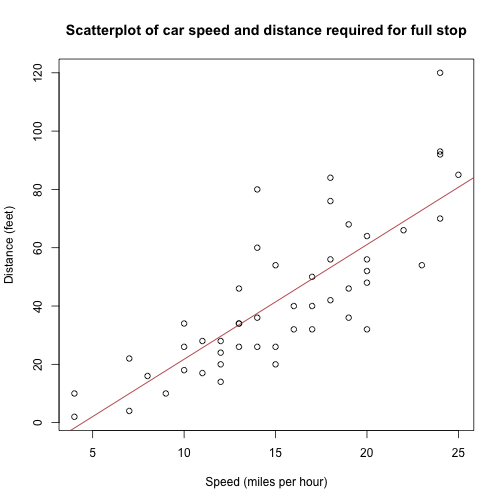
\includegraphics{Scatterplot-1.png}
\caption{Scatterplot}\end{figure}

Also included in the scatter plot is a ``best-fit'' regression line that indicates a positive and linear relationship between our two variables. This basic test coupled with the fact that our outcome variable (distance) is continuous suggests that an appropriate model to use is least squares regression.

To fit this model to our data, we must first create Zelig least squares object, then specify our model, and finally regress distance on speed to estimate the relationship between speed and distance:

\begin{Verbatim}[commandchars=\\\{\}]
\PYG{c+c1}{\PYGZsh{} load dataset (when you install R, example datasets are also installed)}
data\PYG{p}{(}cars\PYG{p}{)}
\PYG{c+c1}{\PYGZsh{} initialize Zelig5 least squares object}
z5 \PYG{o}{\PYGZlt{}\PYGZhy{}} zls\PYG{o}{\PYGZdl{}}new\PYG{p}{(}\PYG{p}{)}
\PYG{c+c1}{\PYGZsh{} estimate ls model}
z5\PYG{o}{\PYGZdl{}}zelig\PYG{p}{(}dist \PYG{o}{\PYGZti{}} speed\PYG{p}{,} data \PYG{o}{=} cars\PYG{p}{)}
\PYG{c+c1}{\PYGZsh{} you can now get model summary estimates}
summary\PYG{p}{(}z5\PYG{p}{)}
\end{Verbatim}

\begin{Verbatim}[commandchars=\\\{\}]
\PYG{c}{\PYGZsh{}\PYGZsh{} Model:}
\PYG{c}{\PYGZsh{}\PYGZsh{} \PYGZdl{}by}
\PYG{c}{\PYGZsh{}\PYGZsh{} [1] 1}
\PYG{c}{\PYGZsh{}\PYGZsh{}}
\PYG{c}{\PYGZsh{}\PYGZsh{}}
\PYG{c}{\PYGZsh{}\PYGZsh{} Call:}
\PYG{c}{\PYGZsh{}\PYGZsh{} stats::lm(formula = dist \PYGZti{} speed, data = .)}
\PYG{c}{\PYGZsh{}\PYGZsh{}}
\PYG{c}{\PYGZsh{}\PYGZsh{} Coefficients:}
\PYG{c}{\PYGZsh{}\PYGZsh{} (Intercept)        speed}
\PYG{c}{\PYGZsh{}\PYGZsh{}     \PYGZhy{}17.579        3.932}
\PYG{c}{\PYGZsh{}\PYGZsh{}}
\PYG{c}{\PYGZsh{}\PYGZsh{} Next step: Use \PYGZsq{}setx\PYGZsq{} method}
\end{Verbatim}

So what do our model estimates tell us? First off, we can see that the positive 3.93 estimate for speed suggests a positive relationship between speed and distance a car needs to stop. That is, the faster a car is going, the longer the distance it needs to come to a full stop. In particular, we would interpret this coefficient as a one unit increase in speed (e.g., mph) leads to a 3 unit increase in distance (e.g., miles) needed for a car to stop. This interpretation is not very intuitive, however, and we might be interested in answering a particular question such as how much more distance does a car need to stop if it traveling 30 versus 50 miles per hour.

Zelig makes this simple, by automating the translation of model estimates in interpretable quantities of interest (more on this below) using Monte Carlo simulations. To get this process started we need to set explanatory variables in our model (i.e., speed) using the \code{\$setx()} method:

\begin{Verbatim}[commandchars=\\\{\}]
\PYG{c+c1}{\PYGZsh{} set speed to 30}
z5\PYG{o}{\PYGZdl{}}setx\PYG{p}{(}speed \PYG{o}{=} \PYG{l+m}{30}\PYG{p}{)}

\PYG{c+c1}{\PYGZsh{} set speed to 50}
z5\PYG{o}{\PYGZdl{}}setx1\PYG{p}{(}speed \PYG{o}{=} \PYG{l+m}{50}\PYG{p}{)}
\end{Verbatim}

Now that we've set our variables, all we have to do is run our simulations:

\begin{Verbatim}[commandchars=\\\{\}]
\PYG{c+c1}{\PYGZsh{} run simulations and estimate quantities of interest}
z5\PYG{o}{\PYGZdl{}}sim\PYG{p}{(}\PYG{p}{)}
z5
\end{Verbatim}

\begin{Verbatim}[commandchars=\\\{\}]
\PYG{c}{\PYGZsh{}\PYGZsh{}}
\PYG{c}{\PYGZsh{}\PYGZsh{}  sim x :}
\PYG{c}{\PYGZsh{}\PYGZsh{}  \PYGZhy{}\PYGZhy{}\PYGZhy{}\PYGZhy{}\PYGZhy{}}
\PYG{c}{\PYGZsh{}\PYGZsh{} ev}
\PYG{c}{\PYGZsh{}\PYGZsh{}       mean       sd     50\PYGZpc{}    2.5\PYGZpc{}    97.5\PYGZpc{}}
\PYG{c}{\PYGZsh{}\PYGZsh{} 1 100.0594 6.588758 100.467 86.9325 112.5575}
\PYG{c}{\PYGZsh{}\PYGZsh{} pv}
\PYG{c}{\PYGZsh{}\PYGZsh{}       mean       sd     50\PYGZpc{}    2.5\PYGZpc{}    97.5\PYGZpc{}}
\PYG{c}{\PYGZsh{}\PYGZsh{} 1 100.0594 6.588758 100.467 86.9325 112.5575}
\PYG{c}{\PYGZsh{}\PYGZsh{}}
\PYG{c}{\PYGZsh{}\PYGZsh{}  sim x1 :}
\PYG{c}{\PYGZsh{}\PYGZsh{}  \PYGZhy{}\PYGZhy{}\PYGZhy{}\PYGZhy{}\PYGZhy{}}
\PYG{c}{\PYGZsh{}\PYGZsh{} ev}
\PYG{c}{\PYGZsh{}\PYGZsh{}       mean       sd      50\PYGZpc{}    2.5\PYGZpc{}    97.5\PYGZpc{}}
\PYG{c}{\PYGZsh{}\PYGZsh{} 1 178.2301 14.75085 178.8296 147.661 205.8809}
\PYG{c}{\PYGZsh{}\PYGZsh{} pv}
\PYG{c}{\PYGZsh{}\PYGZsh{}       mean       sd      50\PYGZpc{}    2.5\PYGZpc{}    97.5\PYGZpc{}}
\PYG{c}{\PYGZsh{}\PYGZsh{} 1 178.2301 14.75085 178.8296 147.661 205.8809}
\PYG{c}{\PYGZsh{}\PYGZsh{} fd}
\PYG{c}{\PYGZsh{}\PYGZsh{}       mean       sd      50\PYGZpc{}     2.5\PYGZpc{}    97.5\PYGZpc{}}
\PYG{c}{\PYGZsh{}\PYGZsh{} 1 78.17075 8.375725 78.46994 60.38378 93.58789}
\end{Verbatim}

Now we've estimated a model and calculated interpretable estimates at two speeds (30 versus 50 mph). What can we do with them? Zelig gives you access to estimated quantities of interest and makes plotting and presenting them particularly easy.


\bigskip\hrule{}\bigskip


\textbf{Quantities of Interest}

As mentioned earlier, a major feature of Zelig is the translation of model estimates into easy to interpret quantities of interest (QIs). These QIs (e.g., expected and predicted values) can be accessed via the \code{\$sim.out} field:

\begin{Verbatim}[commandchars=\\\{\}]
z5\PYG{o}{\PYGZdl{}}sim.out
\end{Verbatim}

\begin{Verbatim}[commandchars=\\\{\}]
\PYG{c}{\PYGZsh{}\PYGZsh{} \PYGZdl{}x}
\PYG{c}{\PYGZsh{}\PYGZsh{} Source: local data frame [1 x 2]}
\PYG{c}{\PYGZsh{}\PYGZsh{} Groups: \PYGZlt{}by row\PYGZgt{}}
\PYG{c}{\PYGZsh{}\PYGZsh{}}
\PYG{c}{\PYGZsh{}\PYGZsh{}              ev            pv}
\PYG{c}{\PYGZsh{}\PYGZsh{} 1 \PYGZlt{}dbl[1000,1]\PYGZgt{} \PYGZlt{}dbl[1000,1]\PYGZgt{}}
\PYG{c}{\PYGZsh{}\PYGZsh{}}
\PYG{c}{\PYGZsh{}\PYGZsh{} \PYGZdl{}x1}
\PYG{c}{\PYGZsh{}\PYGZsh{} Source: local data frame [1 x 3]}
\PYG{c}{\PYGZsh{}\PYGZsh{} Groups: \PYGZlt{}by row\PYGZgt{}}
\PYG{c}{\PYGZsh{}\PYGZsh{}}
\PYG{c}{\PYGZsh{}\PYGZsh{}              ev            pv            fd}
\PYG{c}{\PYGZsh{}\PYGZsh{} 1 \PYGZlt{}dbl[1000,1]\PYGZgt{} \PYGZlt{}dbl[1000,1]\PYGZgt{} \PYGZlt{}dbl[1000,1]\PYGZgt{}}
\end{Verbatim}


\bigskip\hrule{}\bigskip


\textbf{Plots}

A second major Zelig feature is how easy it is to plot QIs for presentation in slides or an article. Using the \code{plot()} function on the \code{z5\$s.out} will produce ready-to-use plots with labels and confidence intervals.

\emph{Plots of QI's:}

\begin{Verbatim}[commandchars=\\\{\}]
z5\PYG{o}{\PYGZdl{}}graph\PYG{p}{(}\PYG{p}{)}
\end{Verbatim}
\begin{figure}[htbp]
\centering
\capstart

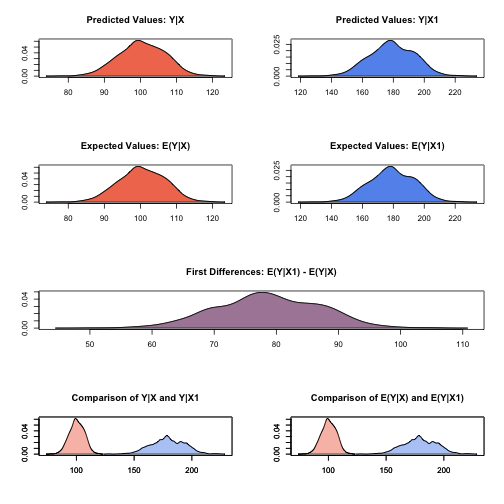
\includegraphics{QIs-1.png}
\caption{QIs}\end{figure}


\bigskip\hrule{}\bigskip


\textbf{Help}

Finally, model documentation can be accessed using the \code{z5\$help()} method after a model object has been initialized:

\begin{Verbatim}[commandchars=\\\{\}]
\PYG{c+c1}{\PYGZsh{} documentation for least squares model}
z5 \PYG{o}{\PYGZlt{}\PYGZhy{}} zls\PYG{o}{\PYGZdl{}}new\PYG{p}{(}\PYG{p}{)}
z5\PYG{o}{\PYGZdl{}}help\PYG{p}{(}\PYG{p}{)}

\PYG{c+c1}{\PYGZsh{} documentation for logistic regression}
z5 \PYG{o}{\PYGZlt{}\PYGZhy{}} zlogit\PYG{o}{\PYGZdl{}}new\PYG{p}{(}\PYG{p}{)}
z5\PYG{o}{\PYGZdl{}}help\PYG{p}{(}\PYG{p}{)}
\end{Verbatim}


\chapter{Model Reference and Vignettes}
\label{vignette:vignettes}\label{vignette:model-reference-and-vignettes}\label{vignette::doc}
This section includes technical information on the models currently implemented in Zelig (5.0-1). This includes a reference with a list of supported models as well as individual model vignettes with detailed information on the model, quantities of interest and syntax.


\section{Reference}
\label{vignette:reference}
The following models are currently supported in Zelig 5.0-1:
\begin{itemize}
\item {} 
{\hyperref[zelig-exp:zexp]{\emph{Exponential Regression}}}: \code{zexp\$new()}

\item {} 
{\hyperref[zelig-gamma:zgamma]{\emph{Gamma Regression}}}: \code{zgamma()}

\item {} 
{\hyperref[zelig-logit:zlogit]{\emph{Logistic Regression}}}: \code{zlogit\$new()}

\item {} 
{\hyperref[zelig-lognorm:zlognorm]{\emph{Log Normal Regression}}}: \code{zlognorm\$new()}

\item {} 
{\hyperref[zelig-ls:zls]{\emph{Least Squares Regression}}}: \code{zls\$new()}

\item {} 
{\hyperref[zelig-negbin:znegbin]{\emph{Negative Binomial Regression}}}: \code{zbinom\$new()}

\item {} 
{\hyperref[zelig-normal:znorm]{\emph{Normal Regression}}}: \code{znormal\$new()}

\item {} 
{\hyperref[zelig-poisson:zpoisson]{\emph{Poisson Regression}}}: \code{zpoisson\$new()}

\item {} 
{\hyperref[zelig-probit:zprobit]{\emph{Probit Regression}}}: \code{zprobit\$new()}

\item {} 
{\hyperref[zelig-relogit:zrelogit]{\emph{Rare Events Logistic Regression}}}: \code{zrelogit\$new()}

\item {} 
{\hyperref[zelig-tobit:ztobit]{\emph{Tobit Regression}}}: \code{ztobit\$new()}

\item {} 
{\hyperref[zelig-factorbayes:zfactorbayes]{\emph{Bayesian Factor Analysis}}}: \code{zfactorbayes\$new()}

\item {} 
{\hyperref[zelig-mlogitbayes:zmlogitbayes]{\emph{Bayesian Multinomial Logistic Regression}}}: \code{zmlogitbayes\$new()}

\item {} 
{\hyperref[zelig-oprobitbayes:zoprobitbayes]{\emph{Bayesian Ordered Probit Regression}}}: \code{zoprobitbayes()}

\item {} 
{\hyperref[zelig-poissonbayes:zpoissonbayes]{\emph{Bayesian Poisson Regression}}}: \code{zpoissonbayes()}

\item {} 
{\hyperref[zelig-probitbayes:zprobitbayes]{\emph{Bayesian Probit Regression}}}: \code{zprobitbayes()}

\end{itemize}


\bigskip\hrule{}\bigskip



\section{zelig-exp}
\label{vignette:zelig-exp}\label{vignette:zexp}
Exponential Regression for Duration Dependent Variables

Use the exponential duration regression model if you have a dependent
variable representing a duration (time until an event). The model
assumes a constant hazard rate for all events. The dependent variable
may be censored (for observations have not yet been completed when data
were collected).


\subsection{Syntax}
\label{vignette:syntax}
With reference classes:

\begin{Verbatim}[commandchars=\\\{\}]
z5 \PYG{o}{\PYGZlt{}\PYGZhy{}} zexp\PYG{o}{\PYGZdl{}}new\PYG{p}{(}\PYG{p}{)}
z5\PYG{o}{\PYGZdl{}}zelig\PYG{p}{(}Surv\PYG{p}{(}Y\PYG{p}{,} C\PYG{p}{)} \PYG{o}{\PYGZti{}} X\PYG{p}{,} data \PYG{o}{=} mydata\PYG{p}{)}
z5\PYG{o}{\PYGZdl{}}setx\PYG{p}{(}\PYG{p}{)}
z5\PYG{o}{\PYGZdl{}}sim\PYG{p}{(}\PYG{p}{)}
\end{Verbatim}

With the Zelig 4 compatibility wrappers:

\begin{Verbatim}[commandchars=\\\{\}]
z.out \PYG{o}{\PYGZlt{}\PYGZhy{}} zelig\PYG{p}{(}Surv\PYG{p}{(}Y\PYG{p}{,} C\PYG{p}{)} \PYG{o}{\PYGZti{}} X\PYG{p}{,} model \PYG{o}{=} \PYG{l+s}{\PYGZdq{}}\PYG{l+s}{exp\PYGZdq{}}\PYG{p}{,} data \PYG{o}{=} mydata\PYG{p}{)}
x.out \PYG{o}{\PYGZlt{}\PYGZhy{}} setx\PYG{p}{(}z.out\PYG{p}{)}
s.out \PYG{o}{\PYGZlt{}\PYGZhy{}} sim\PYG{p}{(}z.out\PYG{p}{,} x \PYG{o}{=} x.out\PYG{p}{)}
\end{Verbatim}

Exponential models require that the dependent variable be in the form
Surv(Y, C), where Y and C are vectors of length \(n\). For each
observation \(i\) in 1, …, \(n\), the value \(y_i\) is the
duration (lifetime, for example), and the associated \(c_i\) is a
binary variable such that \(c_i = 1\) if the duration is not
censored (\emph{e.g.}, the subject dies during the study) or \(c_i = 0\)
if the duration is censored (\emph{e.g.}, the subject is still alive at the
end of the study and is know to live at least as long as \(y_i\)).
If \(c_i\) is omitted, all Y are assumed to be completed; that is,
time defaults to 1 for all observations.


\subsection{Input Values}
\label{vignette:input-values}
In addition to the standard inputs, zelig() takes the following
additional options for exponential regression:
\begin{itemize}
\item {} 
robust: defaults to FALSE. If TRUE, zelig() computes robust standard
errors based on sandwich estimators (see and ) and the options
selected in cluster.

\item {} 
cluster: if robust = TRUE, you may select a variable to define groups
of correlated observations. Let x3 be a variable that consists of
either discrete numeric values, character strings, or factors that
define strata. Then

\end{itemize}

\begin{Verbatim}[commandchars=\\\{\}]
z.out \PYG{o}{\PYGZlt{}\PYGZhy{}} zelig\PYG{p}{(}y \PYG{o}{\PYGZti{}} x1 \PYG{o}{+} x2\PYG{p}{,} robust \PYG{o}{=} \PYG{k+kc}{TRUE}\PYG{p}{,} cluster \PYG{o}{=} \PYG{l+s}{\PYGZdq{}}\PYG{l+s}{x3\PYGZdq{}}\PYG{p}{,}
                        model \PYG{o}{=} \PYG{l+s}{\PYGZdq{}}\PYG{l+s}{exp\PYGZdq{}}\PYG{p}{,} data \PYG{o}{=} mydata\PYG{p}{)}
\end{Verbatim}

means that the observations can be correlated within the strata
defined by the variable x3, and that robust standard errors should be
calculated according to those clusters. If robust = TRUE but cluster
is not specified, zelig() assumes that each observation falls into
its own cluster.


\subsection{Example}
\label{vignette:example}
Attach the sample data:

\begin{Verbatim}[commandchars=\\\{\}]
data\PYG{p}{(}coalition\PYG{p}{)}
\end{Verbatim}

Estimate the model:

\begin{Verbatim}[commandchars=\\\{\}]
z.out \PYG{o}{\PYGZlt{}\PYGZhy{}} zelig\PYG{p}{(}Surv\PYG{p}{(}duration\PYG{p}{,} ciep12\PYG{p}{)} \PYG{o}{\PYGZti{}} fract \PYG{o}{+} numst2\PYG{p}{,} model \PYG{o}{=} \PYG{l+s}{\PYGZdq{}}\PYG{l+s}{exp\PYGZdq{}}\PYG{p}{,} data \PYG{o}{=} coalition\PYG{p}{)}
\end{Verbatim}

\begin{Verbatim}[commandchars=\\\{\}]
\PYG{c}{\PYGZsh{}\PYGZsh{} How to cite this model in Zelig:}
\PYG{c}{\PYGZsh{}\PYGZsh{}   Olivia Lau, Kosuke Imai, Gary King. 2011.}
\PYG{c}{\PYGZsh{}\PYGZsh{}   exp: Exponential Regression for Duration Dependent Variables}
\PYG{c}{\PYGZsh{}\PYGZsh{}   in Kosuke Imai, Gary King, and Olivia Lau, \PYGZdq{}Zelig: Everyone\PYGZsq{}s Statistical Software,\PYGZdq{}}
\PYG{c}{\PYGZsh{}\PYGZsh{}   http://zeligproject.org/}
\end{Verbatim}

View the regression output:

\begin{Verbatim}[commandchars=\\\{\}]
summary\PYG{p}{(}z.out\PYG{p}{)}
\end{Verbatim}

\begin{Verbatim}[commandchars=\\\{\}]
\PYG{c}{\PYGZsh{}\PYGZsh{} Model:}
\PYG{c}{\PYGZsh{}\PYGZsh{} \PYGZdl{}by}
\PYG{c}{\PYGZsh{}\PYGZsh{} [1] 1}
\PYG{c}{\PYGZsh{}\PYGZsh{}}
\PYG{c}{\PYGZsh{}\PYGZsh{} Call:}
\PYG{c}{\PYGZsh{}\PYGZsh{} survival::survreg(formula = Surv(duration, ciep12) \PYGZti{} fract +}
\PYG{c}{\PYGZsh{}\PYGZsh{}     numst2, data = ., dist = \PYGZdq{}exponential\PYGZdq{}, model = FALSE)}
\PYG{c}{\PYGZsh{}\PYGZsh{}}
\PYG{c}{\PYGZsh{}\PYGZsh{} Coefficients:}
\PYG{c}{\PYGZsh{}\PYGZsh{}  (Intercept)        fract       numst2}
\PYG{c}{\PYGZsh{}\PYGZsh{}  5.535872596 \PYGZhy{}0.003908965  0.461179302}
\PYG{c}{\PYGZsh{}\PYGZsh{}}
\PYG{c}{\PYGZsh{}\PYGZsh{} Scale fixed at 1}
\PYG{c}{\PYGZsh{}\PYGZsh{}}
\PYG{c}{\PYGZsh{}\PYGZsh{} Loglik(model)= \PYGZhy{}1077.4   Loglik(intercept only)= \PYGZhy{}1100.7}
\PYG{c}{\PYGZsh{}\PYGZsh{}  Chisq= 46.66 on 2 degrees of freedom, p= 7.4e\PYGZhy{}11}
\PYG{c}{\PYGZsh{}\PYGZsh{} n= 314}
\PYG{c}{\PYGZsh{}\PYGZsh{} Next step: Use \PYGZsq{}setx\PYGZsq{} method}
\end{Verbatim}

Set the baseline values (with the ruling coalition in the minority) and
the alternative values (with the ruling coalition in the majority) for
X:

\begin{Verbatim}[commandchars=\\\{\}]
x.low \PYG{o}{\PYGZlt{}\PYGZhy{}} setx\PYG{p}{(}z.out\PYG{p}{,} numst2 \PYG{o}{=} \PYG{l+m}{0}\PYG{p}{)}
\end{Verbatim}

\begin{Verbatim}[commandchars=\\\{\}]
\PYG{c}{\PYGZsh{}\PYGZsh{} Error in terms(lm(formula, data), \PYGZdq{}predvars\PYGZdq{}): error in evaluating the argument \PYGZsq{}x\PYGZsq{} in selecting a method for function \PYGZsq{}terms\PYGZsq{}: Error in Ops.Surv(y, z\PYGZdl{}residuals) : Invalid operation on a survival time}
\PYG{c}{\PYGZsh{}\PYGZsh{} Calls: lm \PYGZhy{}\PYGZgt{} lm.fit \PYGZhy{}\PYGZgt{} Ops.Surv}
\end{Verbatim}

\begin{Verbatim}[commandchars=\\\{\}]
x.high \PYG{o}{\PYGZlt{}\PYGZhy{}} setx\PYG{p}{(}z.out\PYG{p}{,} numst2 \PYG{o}{=} \PYG{l+m}{1}\PYG{p}{)}
\end{Verbatim}

\begin{Verbatim}[commandchars=\\\{\}]
\PYG{c}{\PYGZsh{}\PYGZsh{} Error in terms(lm(formula, data), \PYGZdq{}predvars\PYGZdq{}): error in evaluating the argument \PYGZsq{}x\PYGZsq{} in selecting a method for function \PYGZsq{}terms\PYGZsq{}: Error in Ops.Surv(y, z\PYGZdl{}residuals) : Invalid operation on a survival time}
\PYG{c}{\PYGZsh{}\PYGZsh{} Calls: lm \PYGZhy{}\PYGZgt{} lm.fit \PYGZhy{}\PYGZgt{} Ops.Surv}
\end{Verbatim}

Simulate expected values and first differences:

\begin{Verbatim}[commandchars=\\\{\}]
s.out \PYG{o}{\PYGZlt{}\PYGZhy{}} sim\PYG{p}{(}z.out\PYG{p}{,} x \PYG{o}{=} x.low\PYG{p}{,} x1 \PYG{o}{=} x.high\PYG{p}{)}
\end{Verbatim}

Summarize quantities of interest and produce some plots:

\begin{Verbatim}[commandchars=\\\{\}]
summary\PYG{p}{(}s.out\PYG{p}{)}
\end{Verbatim}

\begin{Verbatim}[commandchars=\\\{\}]
\PYG{c}{\PYGZsh{}\PYGZsh{}}
\PYG{c}{\PYGZsh{}\PYGZsh{}  sim x :}
\PYG{c}{\PYGZsh{}\PYGZsh{}  \PYGZhy{}\PYGZhy{}\PYGZhy{}\PYGZhy{}\PYGZhy{}}
\PYG{c}{\PYGZsh{}\PYGZsh{} ev}
\PYG{c}{\PYGZsh{}\PYGZsh{}      mean       sd     50\PYGZpc{}     2.5\PYGZpc{}    97.5\PYGZpc{}}
\PYG{c}{\PYGZsh{}\PYGZsh{} 1 4.61167 0.178409 4.61234 4.253718 4.970509}
\PYG{c}{\PYGZsh{}\PYGZsh{} pv}
\PYG{c}{\PYGZsh{}\PYGZsh{}      mean       sd     50\PYGZpc{}     2.5\PYGZpc{}    97.5\PYGZpc{}}
\PYG{c}{\PYGZsh{}\PYGZsh{} 1 4.61167 0.178409 4.61234 4.253718 4.970509}
\PYG{c}{\PYGZsh{}\PYGZsh{}}
\PYG{c}{\PYGZsh{}\PYGZsh{}  sim x1 :}
\PYG{c}{\PYGZsh{}\PYGZsh{}  \PYGZhy{}\PYGZhy{}\PYGZhy{}\PYGZhy{}\PYGZhy{}}
\PYG{c}{\PYGZsh{}\PYGZsh{} ev}
\PYG{c}{\PYGZsh{}\PYGZsh{}       mean        sd      50\PYGZpc{}    2.5\PYGZpc{}    97.5\PYGZpc{}}
\PYG{c}{\PYGZsh{}\PYGZsh{} 1 5.432936 0.1911714 5.435334 5.03635 5.793026}
\PYG{c}{\PYGZsh{}\PYGZsh{} pv}
\PYG{c}{\PYGZsh{}\PYGZsh{}       mean        sd      50\PYGZpc{}    2.5\PYGZpc{}    97.5\PYGZpc{}}
\PYG{c}{\PYGZsh{}\PYGZsh{} 1 5.432936 0.1911714 5.435334 5.03635 5.793026}
\PYG{c}{\PYGZsh{}\PYGZsh{} fd}
\PYG{c}{\PYGZsh{}\PYGZsh{}        mean        sd       50\PYGZpc{}      2.5\PYGZpc{}    97.5\PYGZpc{}}
\PYG{c}{\PYGZsh{}\PYGZsh{} 1 0.8212663 0.2285222 0.8252123 0.3658387 1.259808}
\end{Verbatim}

\begin{Verbatim}[commandchars=\\\{\}]
plot\PYG{p}{(}s.out\PYG{p}{)}
\end{Verbatim}
\begin{figure}[htbp]
\centering
\capstart

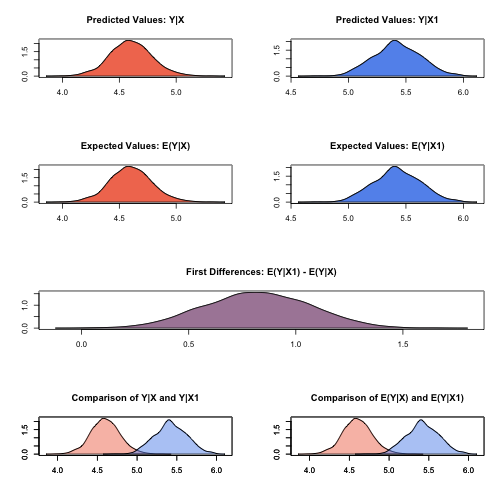
\includegraphics{Zelig-exp-1.png}
\caption{Zelig-exp}\end{figure}


\subsection{Model}
\label{vignette:model}
Let \(Y_i^*\) be the survival time for observation \(i\). This
variable might be censored for some observations at a fixed time
\(y_c\) such that the fully observed dependent variable,
\(Y_i\), is defined as
\begin{gather}
\begin{split}Y_i = \left\{ \begin{array}{ll}
      Y_i^* & \textrm{if }Y_i^* \leq y_c \\
      y_c & \textrm{if }Y_i^* > y_c \\
    \end{array} \right.\end{split}\notag
\end{gather}\begin{itemize}
\item {} 
The \emph{stochastic component} is described by the distribution of the
partially observed variable \(Y^*\). We assume \(Y_i^*\)
follows the exponential distribution whose density function is given
by
\begin{gather}
\begin{split}f(y_i^*\mid \lambda_i) = \frac{1}{\lambda_i} \exp\left(-\frac{y_i^*}{\lambda_i}\right)\end{split}\notag
\end{gather}
for \(y_i^*\ge 0\) and \(\lambda_i>0\). The mean of this
distribution is \(\lambda_i\).

In addition, survival models like the exponential have three
additional properties. The hazard function \(h(t)\) measures the
probability of not surviving past time \(t\) given survival up to
\(t\). In general, the hazard function is equal to
\(f(t)/S(t)\) where the survival function
\(S(t) = 1 - \int_{0}^t f(s) ds\) represents the fraction still
surviving at time \(t\). The cumulative hazard function
\(H(t)\) describes the probability of dying before time
\(t\). In general,
\(H(t)= \int_{0}^{t} h(s) ds = -\log S(t)\). In the case of the
exponential model,
\begin{gather}
\begin{split}\begin{aligned}
h(t) &=& \frac{1}{\lambda_i} \\
S(t) &=& \exp\left( -\frac{t}{\lambda_i} \right) \\
H(t) &=& \frac{t}{\lambda_i}\end{aligned}\end{split}\notag
\end{gather}
For the exponential model, the hazard function \(h(t)\) is
constant over time. The Weibull model and lognormal models allow the
hazard function to vary as a function of elapsed time (see and
respectively).

\item {} 
The \emph{systematic component} \(\lambda_i\) is modeled as
\begin{gather}
\begin{split}\lambda_i = \exp(x_i \beta),\end{split}\notag
\end{gather}
where \(x_i\) is the vector of explanatory variables, and
\(\beta\) is the vector of coefficients.

\end{itemize}


\subsection{Quantities of Interest}
\label{vignette:quantities-of-interest}\begin{itemize}
\item {} 
The expected values (qi\$ev) for the exponential model are simulations
of the expected duration given \(x_i\) and draws of \(\beta\)
from its posterior,
\begin{gather}
\begin{split}E(Y) = \lambda_i = \exp(x_i \beta).\end{split}\notag
\end{gather}
\item {} 
The predicted values (qi\$pr) are draws from the exponential
distribution with rate equal to the expected value.

\item {} 
The first difference (or difference in expected values, qi\$ev.diff),
is
\begin{gather}
\begin{split}\textrm{FD} \; = \; E(Y \mid x_1) - E(Y \mid x),\end{split}\notag
\end{gather}
where \(x\) and \(x_1\) are different vectors of values for
the explanatory variables.

\item {} 
In conditional prediction models, the average expected treatment
effect (att.ev) for the treatment group is
\begin{gather}
\begin{split}\frac{1}{\sum_{i=1}^n t_i}\sum_{i:t_i=1}^n \left\{ Y_i(t_i=1) - E[Y_i(t_i=0)]
  \right\},\end{split}\notag
\end{gather}
where \(t_i\) is a binary explanatory variable defining the
treatment (\(t_i=1\)) and control (\(t_i=0\)) groups. When
\(Y_i(t_i=1)\) is censored rather than observed, we replace it
with a simulation from the model given available knowledge of the
censoring process. Variation in the simulations is due to two
factors: uncertainty in the imputation process for censored
\(y_i^*\) and uncertainty in simulating \(E[Y_i(t_i=0)]\),
the counterfactual expected value of \(Y_i\) for observations in
the treatment group, under the assumption that everything stays the
same except that the treatment indicator is switched to
\(t_i=0\).

\item {} 
In conditional prediction models, the average predicted treatment
effect (att.pr) for the treatment group is
\begin{gather}
\begin{split}\frac{1}{\sum_{i=1}^n t_i}\sum_{i:t_i=1}^n \left\{ Y_i(t_i=1) -
  \widehat{Y_i(t_i=0)} \right\},\end{split}\notag
\end{gather}
where \(t_i\) is a binary explanatory variable defining the
treatment (\(t_i=1\)) and control (\(t_i=0\)) groups. When
\(Y_i(t_i=1)\) is censored rather than observed, we replace it
with a simulation from the model given available knowledge of the
censoring process. Variation in the simulations is due to two
factors: uncertainty in the imputation process for censored
\(y_i^*\) and uncertainty in simulating
\(\widehat{Y_i(t_i=0)}\), the counterfactual predicted value of
\(Y_i\) for observations in the treatment group, under the
assumption that everything stays the same except that the treatment
indicator is switched to \(t_i=0\).

\end{itemize}


\subsection{Output Values}
\label{vignette:output-values}
The output of each Zelig command contains useful information which you
may view. For example, if you run
\code{z.out \textless{}- zelig(Surv(Y, C) \textasciitilde{} X, model = exp, data)}, then you may
examine the available information in \code{z.out} by using
\code{names(z.out)}, see the coefficients by using z.out\$coefficients, and
a default summary of information through \code{summary(z.out)}.


\subsection{See also}
\label{vignette:see-also}
The exponential function is part of the survival library by Terry
Therneau, ported to R by Thomas Lumley. Advanced users may wish to refer
to \code{help(survfit)} in the survival library.


\bigskip\hrule{}\bigskip



\section{zelig-gamma}
\label{vignette:zgamma}\label{vignette:zelig-gamma}
Gamma Regression for Continuous, Positive Dependent Variables

Use the gamma regression model if you have a positive-valued dependent
variable such as the number of years a parliamentary cabinet endures, or
the seconds you can stay airborne while jumping. The gamma distribution
assumes that all waiting times are complete by the end of the study
(censoring is not allowed).


\subsection{Syntax}
\label{vignette:id1}
With reference classes:

\begin{Verbatim}[commandchars=\\\{\}]
z5 \PYG{o}{\PYGZlt{}\PYGZhy{}} zgamma\PYG{o}{\PYGZdl{}}new\PYG{p}{(}\PYG{p}{)}
z5\PYG{o}{\PYGZdl{}}zelig\PYG{p}{(}Y \PYG{o}{\PYGZti{}} X1 \PYG{o}{+} X \PYG{o}{\PYGZti{}} X\PYG{p}{,} data \PYG{o}{=} mydata\PYG{p}{)}
z5\PYG{o}{\PYGZdl{}}setx\PYG{p}{(}\PYG{p}{)}
z5\PYG{o}{\PYGZdl{}}sim\PYG{p}{(}\PYG{p}{)}
\end{Verbatim}

With the Zelig 4 compatibility wrappers:

\begin{Verbatim}[commandchars=\\\{\}]
z.out \PYG{o}{\PYGZlt{}\PYGZhy{}} zelig\PYG{p}{(}Y \PYG{o}{\PYGZti{}} X1 \PYG{o}{+} X2\PYG{p}{,} model \PYG{o}{=} \PYG{l+s}{\PYGZdq{}}\PYG{l+s}{gamma\PYGZdq{}}\PYG{p}{,} data \PYG{o}{=} mydata\PYG{p}{)}
x.out \PYG{o}{\PYGZlt{}\PYGZhy{}} setx\PYG{p}{(}z.out\PYG{p}{)}
s.out \PYG{o}{\PYGZlt{}\PYGZhy{}} sim\PYG{p}{(}z.out\PYG{p}{,} x \PYG{o}{=} x.out\PYG{p}{,} x1 \PYG{o}{=} \PYG{k+kc}{NULL}\PYG{p}{)}
\end{Verbatim}


\subsection{Example}
\label{vignette:id2}
Attach the sample data:

\begin{Verbatim}[commandchars=\\\{\}]
data\PYG{p}{(}coalition\PYG{p}{)}
\end{Verbatim}

Estimate the model:

\begin{Verbatim}[commandchars=\\\{\}]
z.out \PYG{o}{\PYGZlt{}\PYGZhy{}} zelig\PYG{p}{(}duration \PYG{o}{\PYGZti{}} fract \PYG{o}{+} numst2\PYG{p}{,} model \PYG{o}{=} \PYG{l+s}{\PYGZdq{}}\PYG{l+s}{gamma\PYGZdq{}}\PYG{p}{,} data \PYG{o}{=} coalition\PYG{p}{)}
\end{Verbatim}

\begin{Verbatim}[commandchars=\\\{\}]
\PYG{c}{\PYGZsh{}\PYGZsh{} How to cite this model in Zelig:}
\PYG{c}{\PYGZsh{}\PYGZsh{}   Kosuke Imai, Gary King, Olivia Lau. 2007.}
\PYG{c}{\PYGZsh{}\PYGZsh{}   gamma: Gamma Regression for Continuous, Positive Dependent Variables}
\PYG{c}{\PYGZsh{}\PYGZsh{}   in Kosuke Imai, Gary King, and Olivia Lau, \PYGZdq{}Zelig: Everyone\PYGZsq{}s Statistical Software,\PYGZdq{}}
\PYG{c}{\PYGZsh{}\PYGZsh{}   http://zeligproject.org/}
\end{Verbatim}

View the regression output:

\begin{Verbatim}[commandchars=\\\{\}]
summary\PYG{p}{(}z.out\PYG{p}{)}
\end{Verbatim}

\begin{Verbatim}[commandchars=\\\{\}]
\PYG{c}{\PYGZsh{}\PYGZsh{} Model:}
\PYG{c}{\PYGZsh{}\PYGZsh{} \PYGZdl{}by}
\PYG{c}{\PYGZsh{}\PYGZsh{} [1] 1}
\PYG{c}{\PYGZsh{}\PYGZsh{}}
\PYG{c}{\PYGZsh{}\PYGZsh{}}
\PYG{c}{\PYGZsh{}\PYGZsh{} Call:  stats::glm(formula = duration \PYGZti{} fract + numst2, family = Gamma(\PYGZdq{}inverse\PYGZdq{}),}
\PYG{c}{\PYGZsh{}\PYGZsh{}     data = .)}
\PYG{c}{\PYGZsh{}\PYGZsh{}}
\PYG{c}{\PYGZsh{}\PYGZsh{} Coefficients:}
\PYG{c}{\PYGZsh{}\PYGZsh{} (Intercept)        fract       numst2}
\PYG{c}{\PYGZsh{}\PYGZsh{}  \PYGZhy{}0.0129597    0.0001149   \PYGZhy{}0.0173875}
\PYG{c}{\PYGZsh{}\PYGZsh{}}
\PYG{c}{\PYGZsh{}\PYGZsh{} Degrees of Freedom: 313 Total (i.e. Null);  311 Residual}
\PYG{c}{\PYGZsh{}\PYGZsh{} Null Deviance:       300.7}
\PYG{c}{\PYGZsh{}\PYGZsh{} Residual Deviance: 272.2         AIC: 2428}
\PYG{c}{\PYGZsh{}\PYGZsh{} Next step: Use \PYGZsq{}setx\PYGZsq{} method}
\end{Verbatim}

Set the baseline values (with the ruling coalition in the minority) and
the alternative values (with the ruling coalition in the majority) for
X:

\begin{Verbatim}[commandchars=\\\{\}]
x.low \PYG{o}{\PYGZlt{}\PYGZhy{}} setx\PYG{p}{(}z.out\PYG{p}{,} numst2 \PYG{o}{=} \PYG{l+m}{0}\PYG{p}{)}
x.high \PYG{o}{\PYGZlt{}\PYGZhy{}} setx\PYG{p}{(}z.out\PYG{p}{,} numst2 \PYG{o}{=} \PYG{l+m}{1}\PYG{p}{)}
\end{Verbatim}

Simulate expected values (qi\$ev) and first differences (qi\$fd):

\begin{Verbatim}[commandchars=\\\{\}]
s.out \PYG{o}{\PYGZlt{}\PYGZhy{}} sim\PYG{p}{(}z.out\PYG{p}{,} x \PYG{o}{=} x.low\PYG{p}{,} x1 \PYG{o}{=} x.high\PYG{p}{)}
\end{Verbatim}

\begin{Verbatim}[commandchars=\\\{\}]
summary\PYG{p}{(}s.out\PYG{p}{)}
\end{Verbatim}

\begin{Verbatim}[commandchars=\\\{\}]
\PYG{c}{\PYGZsh{}\PYGZsh{}}
\PYG{c}{\PYGZsh{}\PYGZsh{}  sim x :}
\PYG{c}{\PYGZsh{}\PYGZsh{}  \PYGZhy{}\PYGZhy{}\PYGZhy{}\PYGZhy{}\PYGZhy{}}
\PYG{c}{\PYGZsh{}\PYGZsh{} ev}
\PYG{c}{\PYGZsh{}\PYGZsh{}          mean       sd      50\PYGZpc{}     2.5\PYGZpc{}    97.5\PYGZpc{}}
\PYG{c}{\PYGZsh{}\PYGZsh{} [1,] 14.41947 1.064664 14.35618 12.51195 16.63425}
\PYG{c}{\PYGZsh{}\PYGZsh{} pv}
\PYG{c}{\PYGZsh{}\PYGZsh{}          mean       sd      50\PYGZpc{}      2.5\PYGZpc{}    97.5\PYGZpc{}}
\PYG{c}{\PYGZsh{}\PYGZsh{} [1,] 14.21243 12.60368 10.89322 0.6728363 47.30353}
\PYG{c}{\PYGZsh{}\PYGZsh{}}
\PYG{c}{\PYGZsh{}\PYGZsh{}  sim x1 :}
\PYG{c}{\PYGZsh{}\PYGZsh{}  \PYGZhy{}\PYGZhy{}\PYGZhy{}\PYGZhy{}\PYGZhy{}}
\PYG{c}{\PYGZsh{}\PYGZsh{} ev}
\PYG{c}{\PYGZsh{}\PYGZsh{}          mean       sd      50\PYGZpc{}    2.5\PYGZpc{}    97.5\PYGZpc{}}
\PYG{c}{\PYGZsh{}\PYGZsh{} [1,] 19.19869 1.133553 19.11127 17.1843 21.62197}
\PYG{c}{\PYGZsh{}\PYGZsh{} pv}
\PYG{c}{\PYGZsh{}\PYGZsh{}          mean       sd      50\PYGZpc{}      2.5\PYGZpc{}    97.5\PYGZpc{}}
\PYG{c}{\PYGZsh{}\PYGZsh{} [1,] 18.60736 16.66119 13.88459 0.9246994 61.53045}
\PYG{c}{\PYGZsh{}\PYGZsh{} fd}
\PYG{c}{\PYGZsh{}\PYGZsh{}          mean       sd      50\PYGZpc{}     2.5\PYGZpc{}    97.5\PYGZpc{}}
\PYG{c}{\PYGZsh{}\PYGZsh{} [1,] 4.779217 1.535785 4.734045 1.825047 7.751185}
\end{Verbatim}

\begin{Verbatim}[commandchars=\\\{\}]
plot\PYG{p}{(}s.out\PYG{p}{)}
\end{Verbatim}
\begin{figure}[htbp]
\centering
\capstart

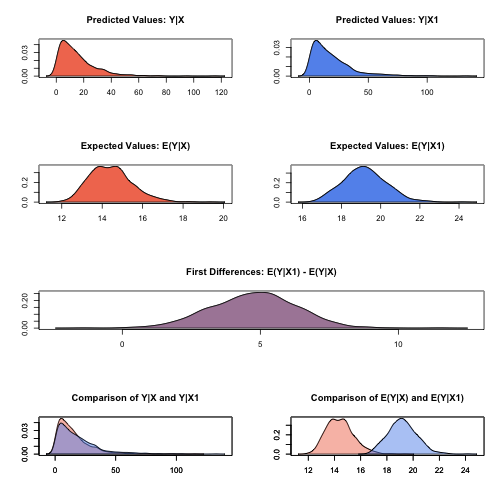
\includegraphics{Zelig-gamma-1.png}
\caption{Zelig-gamma}\end{figure}


\subsection{Model}
\label{vignette:id3}\begin{itemize}
\item {} 
The Gamma distribution with scale parameter \(\alpha\) has a
\emph{stochastic component}:
\begin{gather}
\begin{split}\begin{aligned}
Y &\sim& \textrm{Gamma}(y_i \mid \lambda_i, \alpha) \\
f(y)  &=& \frac{1}{\alpha^{\lambda_i} \, \Gamma \lambda_i} \, y_i^{\lambda_i
  - 1} \exp -\left\{ \frac{y_i}{\alpha} \right\}\end{aligned}\end{split}\notag
\end{gather}
\begin{DUlineblock}{0em}
\item[] for \(\alpha, \lambda_i, y_i > 0\).
\end{DUlineblock}

\item {} 
The \emph{systematic component} is given by
\begin{gather}
\begin{split}\lambda_i = \frac{1}{x_i \beta}\end{split}\notag
\end{gather}
\end{itemize}


\subsection{Quantities of Interest}
\label{vignette:id4}\begin{itemize}
\item {} 
The expected values (qi\$ev) are simulations of the mean of the
stochastic component given draws of \(\alpha\) and \(\beta\)
from their posteriors:
\begin{gather}
\begin{split}E(Y) = \alpha \lambda_i.\end{split}\notag
\end{gather}
\item {} 
The predicted values (qi\$pr) are draws from the gamma distribution
for each given set of parameters \((\alpha, \lambda_i)\).

\item {} 
If x1 is specified, sim() also returns the differences in the
expected values (qi\$fd),
\begin{gather}
\begin{split}E(Y \mid x_1) -
  E(Y \mid x)\end{split}\notag
\end{gather}
.

\item {} 
In conditional prediction models, the average expected treatment
effect (att.ev) for the treatment group is
\begin{gather}
\begin{split}\frac{1}{\sum_{i=1}^n t_i}\sum_{i:t_i=1}^n \left\{ Y_i(t_i=1) -
      E[Y_i(t_i=0)] \right\},\end{split}\notag
\end{gather}
where \(t_i\) is a binary explanatory variable defining the
treatment (\(t_i=1\)) and control (\(t_i=0\)) groups.
Variation in the simulations are due to uncertainty in simulating
\(E[Y_i(t_i=0)]\), the counterfactual expected value of
\(Y_i\) for observations in the treatment group, under the
assumption that everything stays the same except that the treatment
indicator is switched to \(t_i=0\).

\item {} 
In conditional prediction models, the average predicted treatment
effect (att.pr) for the treatment group is
\begin{gather}
\begin{split}\frac{1}{\sum_{i=1}^n t_i}\sum_{i:t_i=1}^n \left\{ Y_i(t_i=1) -
      \widehat{Y_i(t_i=0)} \right\},\end{split}\notag
\end{gather}
where \(t_i\) is a binary explanatory variable defining the
treatment (\(t_i=1\)) and control (\(t_i=0\)) groups.
Variation in the simulations are due to uncertainty in simulating
\(\widehat{Y_i(t_i=0)}\), the counterfactual predicted value of
\(Y_i\) for observations in the treatment group, under the
assumption that everything stays the same except that the treatment
indicator is switched to \(t_i=0\).

\end{itemize}


\subsection{Output Values}
\label{vignette:id5}
The output of each Zelig command contains useful information which you
may view. For example, if you run
\code{z.out \textless{}- zelig(y \textasciitilde{} x, model = gamma, data)}, then you may examine the
available information in \code{z.out} by using \code{names(z.out)}, see the
coefficients by using z.out\$coefficients, and a default summary of
information through \code{summary(z.out)}.


\subsection{See also}
\label{vignette:id6}
The gamma model is part of the stats package. Advanced users may
wish to refer to \code{help(glm)} and \code{help(family)}.


\bigskip\hrule{}\bigskip



\section{zelig-logit}
\label{vignette:zelig-logit}\label{vignette:zlogit}
Logistic Regression for Dichotomous Dependent Variables

Logistic regression specifies a dichotomous dependent variable as a
function of a set of explanatory variables.


\subsection{Syntax}
\label{vignette:id7}
With reference classes:

\begin{Verbatim}[commandchars=\\\{\}]
z5 \PYG{o}{\PYGZlt{}\PYGZhy{}} zlogit\PYG{o}{\PYGZdl{}}new\PYG{p}{(}\PYG{p}{)}
z5\PYG{o}{\PYGZdl{}}zelig\PYG{p}{(}Y \PYG{o}{\PYGZti{}} X1 \PYG{o}{+} X \PYG{o}{\PYGZti{}} X\PYG{p}{,} data \PYG{o}{=} mydata\PYG{p}{)}
z5\PYG{o}{\PYGZdl{}}setx\PYG{p}{(}\PYG{p}{)}
z5\PYG{o}{\PYGZdl{}}sim\PYG{p}{(}\PYG{p}{)}
\end{Verbatim}

With the Zelig 4 compatibility wrappers:

\begin{Verbatim}[commandchars=\\\{\}]
z.out \PYG{o}{\PYGZlt{}\PYGZhy{}} zelig\PYG{p}{(}Y \PYG{o}{\PYGZti{}} X1 \PYG{o}{+} X2\PYG{p}{,} model \PYG{o}{=} \PYG{l+s}{\PYGZdq{}}\PYG{l+s}{logit\PYGZdq{}}\PYG{p}{,} data \PYG{o}{=} mydata\PYG{p}{)}
x.out \PYG{o}{\PYGZlt{}\PYGZhy{}} setx\PYG{p}{(}z.out\PYG{p}{)}
s.out \PYG{o}{\PYGZlt{}\PYGZhy{}} sim\PYG{p}{(}z.out\PYG{p}{,} x \PYG{o}{=} x.out\PYG{p}{,} x1 \PYG{o}{=} \PYG{k+kc}{NULL}\PYG{p}{)}
\end{Verbatim}


\subsection{Examples}
\label{vignette:examples}

\subsubsection{Basic Example}
\label{vignette:basic-example}
Attaching the sample turnout dataset:

\begin{Verbatim}[commandchars=\\\{\}]
data\PYG{p}{(}turnout\PYG{p}{)}
\end{Verbatim}

Estimating parameter values for the logistic regression:

\begin{Verbatim}[commandchars=\\\{\}]
z.out1 \PYG{o}{\PYGZlt{}\PYGZhy{}} zelig\PYG{p}{(}vote \PYG{o}{\PYGZti{}} age \PYG{o}{+} race\PYG{p}{,} model \PYG{o}{=} \PYG{l+s}{\PYGZdq{}}\PYG{l+s}{logit\PYGZdq{}}\PYG{p}{,} data \PYG{o}{=} turnout\PYG{p}{)}
\end{Verbatim}

\begin{Verbatim}[commandchars=\\\{\}]
\PYG{c}{\PYGZsh{}\PYGZsh{} How to cite this model in Zelig:}
\PYG{c}{\PYGZsh{}\PYGZsh{}   Kosuke Imai, Gary King, Olivia Lau. 2007.}
\PYG{c}{\PYGZsh{}\PYGZsh{}   logit: Logistic Regression for Dichotomous Dependent Variables}
\PYG{c}{\PYGZsh{}\PYGZsh{}   in Kosuke Imai, Gary King, and Olivia Lau, \PYGZdq{}Zelig: Everyone\PYGZsq{}s Statistical Software,\PYGZdq{}}
\PYG{c}{\PYGZsh{}\PYGZsh{}   http://zeligproject.org/}
\end{Verbatim}

Setting values for the explanatory variables:

\begin{Verbatim}[commandchars=\\\{\}]
x.out1 \PYG{o}{\PYGZlt{}\PYGZhy{}} setx\PYG{p}{(}z.out1\PYG{p}{,} age \PYG{o}{=} \PYG{l+m}{36}\PYG{p}{,} race \PYG{o}{=} \PYG{l+s}{\PYGZdq{}}\PYG{l+s}{white\PYGZdq{}}\PYG{p}{)}
\end{Verbatim}

Simulating quantities of interest from the posterior distribution.

\begin{Verbatim}[commandchars=\\\{\}]
s.out1 \PYG{o}{\PYGZlt{}\PYGZhy{}} sim\PYG{p}{(}z.out1\PYG{p}{,} x \PYG{o}{=} x.out1\PYG{p}{)}
\end{Verbatim}

\begin{Verbatim}[commandchars=\\\{\}]
summary\PYG{p}{(}s.out1\PYG{p}{)}
\end{Verbatim}

\begin{Verbatim}[commandchars=\\\{\}]
\PYG{c}{\PYGZsh{}\PYGZsh{}}
\PYG{c}{\PYGZsh{}\PYGZsh{}  sim x :}
\PYG{c}{\PYGZsh{}\PYGZsh{}  \PYGZhy{}\PYGZhy{}\PYGZhy{}\PYGZhy{}\PYGZhy{}}
\PYG{c}{\PYGZsh{}\PYGZsh{} ev}
\PYG{c}{\PYGZsh{}\PYGZsh{}           mean         sd      50\PYGZpc{}     2.5\PYGZpc{}     97.5\PYGZpc{}}
\PYG{c}{\PYGZsh{}\PYGZsh{} [1,] 0.7479394 0.01193434 0.748012 0.724231 0.7712138}
\PYG{c}{\PYGZsh{}\PYGZsh{} pv}
\PYG{c}{\PYGZsh{}\PYGZsh{}          0     1}
\PYG{c}{\PYGZsh{}\PYGZsh{} [1,] 0.278 0.722}
\end{Verbatim}

\begin{Verbatim}[commandchars=\\\{\}]
plot\PYG{p}{(}s.out1\PYG{p}{)}
\end{Verbatim}
\begin{figure}[htbp]
\centering
\capstart


\includegraphics{Zelig-logit-1-1.png}
\caption{Zelig-logit-1}\end{figure}


\subsubsection{Simulating First Differences}
\label{vignette:simulating-first-differences}
Estimating the risk difference (and risk ratio) between low education
(25th percentile) and high education (75th percentile) while all the
other variables held at their default values.

\begin{Verbatim}[commandchars=\\\{\}]
z.out2 \PYG{o}{\PYGZlt{}\PYGZhy{}} zelig\PYG{p}{(}vote \PYG{o}{\PYGZti{}} race \PYG{o}{+} educate\PYG{p}{,} model \PYG{o}{=} \PYG{l+s}{\PYGZdq{}}\PYG{l+s}{logit\PYGZdq{}}\PYG{p}{,} data \PYG{o}{=} turnout\PYG{p}{)}
\end{Verbatim}

\begin{Verbatim}[commandchars=\\\{\}]
\PYG{c}{\PYGZsh{}\PYGZsh{} How to cite this model in Zelig:}
\PYG{c}{\PYGZsh{}\PYGZsh{}   Kosuke Imai, Gary King, Olivia Lau. 2007.}
\PYG{c}{\PYGZsh{}\PYGZsh{}   logit: Logistic Regression for Dichotomous Dependent Variables}
\PYG{c}{\PYGZsh{}\PYGZsh{}   in Kosuke Imai, Gary King, and Olivia Lau, \PYGZdq{}Zelig: Everyone\PYGZsq{}s Statistical Software,\PYGZdq{}}
\PYG{c}{\PYGZsh{}\PYGZsh{}   http://zeligproject.org/}
\end{Verbatim}

\begin{Verbatim}[commandchars=\\\{\}]
x.high \PYG{o}{\PYGZlt{}\PYGZhy{}} setx\PYG{p}{(}z.out2\PYG{p}{,} educate \PYG{o}{=} quantile\PYG{p}{(}turnout\PYG{o}{\PYGZdl{}}educate\PYG{p}{,} prob \PYG{o}{=} \PYG{l+m}{0.75}\PYG{p}{)}\PYG{p}{)}
x.low \PYG{o}{\PYGZlt{}\PYGZhy{}} setx\PYG{p}{(}z.out2\PYG{p}{,} educate \PYG{o}{=} quantile\PYG{p}{(}turnout\PYG{o}{\PYGZdl{}}educate\PYG{p}{,} prob \PYG{o}{=} \PYG{l+m}{0.25}\PYG{p}{)}\PYG{p}{)}
s.out2 \PYG{o}{\PYGZlt{}\PYGZhy{}} sim\PYG{p}{(}z.out2\PYG{p}{,} x \PYG{o}{=} x.high\PYG{p}{,} x1 \PYG{o}{=} x.low\PYG{p}{)}
summary\PYG{p}{(}s.out2\PYG{p}{)}
\end{Verbatim}

\begin{Verbatim}[commandchars=\\\{\}]
\PYG{c}{\PYGZsh{}\PYGZsh{}}
\PYG{c}{\PYGZsh{}\PYGZsh{}  sim x :}
\PYG{c}{\PYGZsh{}\PYGZsh{}  \PYGZhy{}\PYGZhy{}\PYGZhy{}\PYGZhy{}\PYGZhy{}}
\PYG{c}{\PYGZsh{}\PYGZsh{} ev}
\PYG{c}{\PYGZsh{}\PYGZsh{}           mean         sd       50\PYGZpc{}      2.5\PYGZpc{}     97.5\PYGZpc{}}
\PYG{c}{\PYGZsh{}\PYGZsh{} [1,] 0.8221088 0.01046643 0.8225926 0.7989981 0.8425136}
\PYG{c}{\PYGZsh{}\PYGZsh{} pv}
\PYG{c}{\PYGZsh{}\PYGZsh{}          0     1}
\PYG{c}{\PYGZsh{}\PYGZsh{} [1,] 0.172 0.828}
\PYG{c}{\PYGZsh{}\PYGZsh{}}
\PYG{c}{\PYGZsh{}\PYGZsh{}  sim x1 :}
\PYG{c}{\PYGZsh{}\PYGZsh{}  \PYGZhy{}\PYGZhy{}\PYGZhy{}\PYGZhy{}\PYGZhy{}}
\PYG{c}{\PYGZsh{}\PYGZsh{} ev}
\PYG{c}{\PYGZsh{}\PYGZsh{}           mean         sd      50\PYGZpc{}      2.5\PYGZpc{}    97.5\PYGZpc{}}
\PYG{c}{\PYGZsh{}\PYGZsh{} [1,] 0.7091027 0.01317142 0.708915 0.6826494 0.734145}
\PYG{c}{\PYGZsh{}\PYGZsh{} pv}
\PYG{c}{\PYGZsh{}\PYGZsh{}          0     1}
\PYG{c}{\PYGZsh{}\PYGZsh{} [1,] 0.303 0.697}
\PYG{c}{\PYGZsh{}\PYGZsh{} fd}
\PYG{c}{\PYGZsh{}\PYGZsh{}            mean        sd        50\PYGZpc{}       2.5\PYGZpc{}       97.5\PYGZpc{}}
\PYG{c}{\PYGZsh{}\PYGZsh{} [1,] \PYGZhy{}0.1130061 0.0116836 \PYGZhy{}0.1131443 \PYGZhy{}0.1363372 \PYGZhy{}0.09073965}
\end{Verbatim}

\begin{Verbatim}[commandchars=\\\{\}]
plot\PYG{p}{(}s.out2\PYG{p}{)}
\end{Verbatim}
\begin{figure}[htbp]
\centering
\capstart

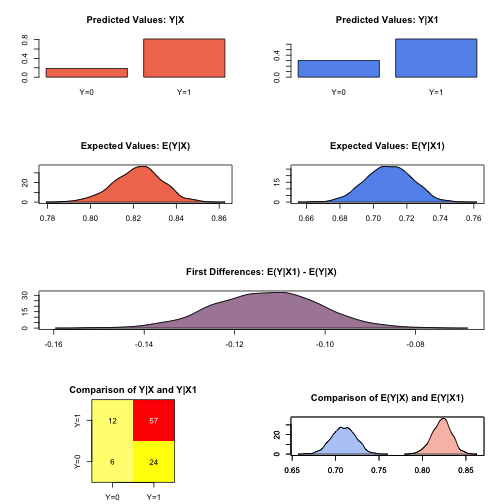
\includegraphics{Zelig-logit-2-1.png}
\caption{Zelig-logit-2}\end{figure}


\subsection{Model}
\label{vignette:id8}
Let \(Y_i\) be the binary dependent variable for observation
\(i\) which takes the value of either 0 or 1.
\begin{itemize}
\item {} 
The \emph{stochastic component} is given by
\begin{gather}
\begin{split}\begin{aligned}
Y_i &\sim& \textrm{Bernoulli}(y_i \mid \pi_i) \\
    &=& \pi_i^{y_i} (1-\pi_i)^{1-y_i}\end{aligned}\end{split}\notag
\end{gather}
where \(\pi_i=\Pr(Y_i=1)\).

\item {} 
The \emph{systematic component} is given by:
\begin{gather}
\begin{split}\pi_i \; = \; \frac{1}{1 + \exp(-x_i \beta)}.\end{split}\notag
\end{gather}
where \(x_i\) is the vector of \(k\) explanatory variables
for observation \(i\) and \(\beta\) is the vector of
coefficients.

\end{itemize}


\subsection{Quantities of Interest}
\label{vignette:id9}\begin{itemize}
\item {} 
The expected values (qi\$ev) for the logit model are simulations of
the predicted probability of a success:
\begin{gather}
\begin{split}E(Y) =
  \pi_i= \frac{1}{1 + \exp(-x_i \beta)},\end{split}\notag
\end{gather}
given draws of \(\beta\) from its sampling distribution.

\item {} 
The predicted values (qi\$pr) are draws from the Binomial distribution
with mean equal to the simulated expected value \(\pi_i\).

\item {} 
The first difference (qi\$fd) for the logit model is defined as
\begin{gather}
\begin{split}\textrm{FD} = \Pr(Y = 1 \mid x_1) - \Pr(Y = 1 \mid x).\end{split}\notag
\end{gather}
\item {} 
The risk ratio (qi\$rr) is defined as
\begin{gather}
\begin{split}\textrm{RR} = \Pr(Y = 1 \mid x_1) \ / \ \Pr(Y = 1 \mid x).\end{split}\notag
\end{gather}
\item {} 
In conditional prediction models, the average expected treatment
effect (att.ev) for the treatment group is
\begin{gather}
\begin{split}\frac{1}{\sum_{i=1}^n t_i}\sum_{i:t_i=1}^n \left\{ Y_i(t_i=1) -
      E[Y_i(t_i=0)] \right\},\end{split}\notag
\end{gather}
where \(t_i\) is a binary explanatory variable defining the
treatment (\(t_i=1\)) and control (\(t_i=0\)) groups.
Variation in the simulations are due to uncertainty in simulating
\(E[Y_i(t_i=0)]\), the counterfactual expected value of
\(Y_i\) for observations in the treatment group, under the
assumption that everything stays the same except that the treatment
indicator is switched to \(t_i=0\).

\item {} 
In conditional prediction models, the average predicted treatment
effect (att.pr) for the treatment group is
\begin{gather}
\begin{split}\frac{1}{\sum_{i=1}^n t_i}\sum_{i:t_i=1}^n \left\{ Y_i(t_i=1) -
      \widehat{Y_i(t_i=0)}\right\},\end{split}\notag
\end{gather}
where \(t_i\) is a binary explanatory variable defining the
treatment (\(t_i=1\)) and control (\(t_i=0\)) groups.
Variation in the simulations are due to uncertainty in simulating
\(\widehat{Y_i(t_i=0)}\), the counterfactual predicted value of
\(Y_i\) for observations in the treatment group, under the
assumption that everything stays the same except that the treatment
indicator is switched to \(t_i=0\).

\end{itemize}


\subsection{Output Values}
\label{vignette:id10}
The output of each Zelig command contains useful information which you
may view. For example, if you run
\code{z.out \textless{}- zelig(y \textasciitilde{} x, model = logit, data)}, then you may examine the
available information in \code{z.out} by using \code{names(z.out)}, see the
coefficients by using z.out\$coefficients, and a default summary of
information through \code{summary(z.out)}.


\subsection{See also}
\label{vignette:id11}
The logit model is part of the stats package. Advanced users may
wish to refer to \code{help(glm)} and \code{help(family)}.


\bigskip\hrule{}\bigskip



\section{zelig-lognorm}
\label{vignette:zelig-lognorm}\label{vignette:zlognorm}
Log-Normal Regression for Duration Dependent Variables

The log-normal model describes an event’s duration, the dependent
variable, as a function of a set of explanatory variables. The
log-normal model may take time censored dependent variables, and allows
the hazard rate to increase and decrease.


\subsection{Syntax}
\label{vignette:id12}
With reference classes:

\begin{Verbatim}[commandchars=\\\{\}]
z5 \PYG{o}{\PYGZlt{}\PYGZhy{}} zlognorm\PYG{o}{\PYGZdl{}}new\PYG{p}{(}\PYG{p}{)}
z5\PYG{o}{\PYGZdl{}}zelig\PYG{p}{(}Surv\PYG{p}{(}Y\PYG{p}{,} C\PYG{p}{)} \PYG{o}{\PYGZti{}} X\PYG{p}{,} data \PYG{o}{=} mydata\PYG{p}{)}
z5\PYG{o}{\PYGZdl{}}setx\PYG{p}{(}\PYG{p}{)}
z5\PYG{o}{\PYGZdl{}}sim\PYG{p}{(}\PYG{p}{)}
\end{Verbatim}

With reference classes:

\begin{Verbatim}[commandchars=\\\{\}]
z5 \PYG{o}{\PYGZlt{}\PYGZhy{}} zlognorm\PYG{o}{\PYGZdl{}}new\PYG{p}{(}\PYG{p}{)}
z5\PYG{o}{\PYGZdl{}}zelig\PYG{p}{(}Surv\PYG{p}{(}Y\PYG{p}{,} C\PYG{p}{)} \PYG{o}{\PYGZti{}} X\PYG{p}{,} data \PYG{o}{=} mydata\PYG{p}{)}
z5\PYG{o}{\PYGZdl{}}setx\PYG{p}{(}\PYG{p}{)}
z5\PYG{o}{\PYGZdl{}}sim\PYG{p}{(}\PYG{p}{)}
\end{Verbatim}

With the Zelig 4 compatibility wrappers:

\begin{Verbatim}[commandchars=\\\{\}]
z.out \PYG{o}{\PYGZlt{}\PYGZhy{}} zelig\PYG{p}{(}Surv\PYG{p}{(}Y\PYG{p}{,} C\PYG{p}{)} \PYG{o}{\PYGZti{}} X\PYG{p}{,} model \PYG{o}{=} \PYG{l+s}{\PYGZdq{}}\PYG{l+s}{lognorm\PYGZdq{}}\PYG{p}{,} data \PYG{o}{=} mydata\PYG{p}{)}
x.out \PYG{o}{\PYGZlt{}\PYGZhy{}} setx\PYG{p}{(}z.out\PYG{p}{)}
s.out \PYG{o}{\PYGZlt{}\PYGZhy{}} sim\PYG{p}{(}z.out\PYG{p}{,} x \PYG{o}{=} x.out\PYG{p}{)}
\end{Verbatim}

Log-normal models require that the dependent variable be in the form
Surv(Y, C), where Y and C are vectors of length \(n\). For each
observation \(i\) in 1, …, \(n\), the value \(y_i\) is the
duration (lifetime, for example) of each subject, and the associated
\(c_i\) is a binary variable such that \(c_i = 1\) if the
duration is not censored (\emph{e.g.}, the subject dies during the study) or
\(c_i = 0\) if the duration is censored (\emph{e.g.}, the subject is
still alive at the end of the study). If \(c_i\) is omitted, all Y
are assumed to be completed; that is, time defaults to 1 for all
observations.


\subsection{Input Values}
\label{vignette:id13}
In addition to the standard inputs, zelig() takes the following
additional options for lognormal regression:
\begin{itemize}
\item {} 
robust: defaults to FALSE. If TRUE, zelig() computes robust standard
errors based on sandwich estimators (see and ) based on the options
in cluster.

\item {} 
cluster: if robust = TRUE, you may select a variable to define groups
of correlated observations. Let x3 be a variable that consists of
either discrete numeric values, character strings, or factors that
define strata. Then

\end{itemize}

\begin{Verbatim}[commandchars=\\\{\}]
z.out \PYG{o}{\PYGZlt{}\PYGZhy{}} zelig\PYG{p}{(}y \PYG{o}{\PYGZti{}} x1 \PYG{o}{+} x2\PYG{p}{,} robust \PYG{o}{=} \PYG{k+kc}{TRUE}\PYG{p}{,} cluster \PYG{o}{=} \PYG{l+s}{\PYGZdq{}}\PYG{l+s}{x3\PYGZdq{}}\PYG{p}{,} model \PYG{o}{=} \PYG{l+s}{\PYGZdq{}}\PYG{l+s}{exp\PYGZdq{}}\PYG{p}{,} data \PYG{o}{=} mydata\PYG{p}{)}
\end{Verbatim}

means that the observations can be correlated within the strata
defined by the variable x3, and that robust standard errors should be
calculated according to those clusters. If robust = TRUE but cluster
is not specified, zelig() assumes that each observation falls into
its own cluster.


\subsection{Example}
\label{vignette:id14}
Attach the sample data:

\begin{Verbatim}[commandchars=\\\{\}]
data\PYG{p}{(}coalition\PYG{p}{)}
\end{Verbatim}

Estimate the model:

\begin{Verbatim}[commandchars=\\\{\}]
z.out \PYG{o}{\PYGZlt{}\PYGZhy{}} zelig\PYG{p}{(}Surv\PYG{p}{(}duration\PYG{p}{,} ciep12\PYG{p}{)} \PYG{o}{\PYGZti{}} fract \PYG{o}{+} numst2\PYG{p}{,} model \PYG{o}{=}\PYG{l+s}{\PYGZdq{}}\PYG{l+s}{lognorm\PYGZdq{}}\PYG{p}{,}  data \PYG{o}{=} coalition\PYG{p}{)}
\end{Verbatim}

\begin{Verbatim}[commandchars=\\\{\}]
\PYG{c}{\PYGZsh{}\PYGZsh{} How to cite this model in Zelig:}
\PYG{c}{\PYGZsh{}\PYGZsh{}   Matthew Owen, Olivia Lau, Kosuke Imai, Gary King. 2007.}
\PYG{c}{\PYGZsh{}\PYGZsh{}   lognorm: Log\PYGZhy{}Normal Regression for Duration Dependent Variables}
\PYG{c}{\PYGZsh{}\PYGZsh{}   in Kosuke Imai, Gary King, and Olivia Lau, \PYGZdq{}Zelig: Everyone\PYGZsq{}s Statistical Software,\PYGZdq{}}
\PYG{c}{\PYGZsh{}\PYGZsh{}   http://zeligproject.org/}
\end{Verbatim}

View the regression output:

\begin{Verbatim}[commandchars=\\\{\}]
summary\PYG{p}{(}z.out\PYG{p}{)}
\end{Verbatim}

\begin{Verbatim}[commandchars=\\\{\}]
\PYG{c}{\PYGZsh{}\PYGZsh{} Model:}
\PYG{c}{\PYGZsh{}\PYGZsh{} \PYGZdl{}by}
\PYG{c}{\PYGZsh{}\PYGZsh{} [1] 1}
\PYG{c}{\PYGZsh{}\PYGZsh{}}
\PYG{c}{\PYGZsh{}\PYGZsh{} Call:}
\PYG{c}{\PYGZsh{}\PYGZsh{} survival::survreg(formula = Surv(duration, ciep12) \PYGZti{} fract +}
\PYG{c}{\PYGZsh{}\PYGZsh{}     numst2, data = ., dist = \PYGZdq{}lognormal\PYGZdq{}, model = FALSE)}
\PYG{c}{\PYGZsh{}\PYGZsh{}}
\PYG{c}{\PYGZsh{}\PYGZsh{} Coefficients:}
\PYG{c}{\PYGZsh{}\PYGZsh{} (Intercept)       fract      numst2}
\PYG{c}{\PYGZsh{}\PYGZsh{}  5.36666977 \PYGZhy{}0.00443755  0.55983251}
\PYG{c}{\PYGZsh{}\PYGZsh{}}
\PYG{c}{\PYGZsh{}\PYGZsh{} Scale= 1.20008}
\PYG{c}{\PYGZsh{}\PYGZsh{}}
\PYG{c}{\PYGZsh{}\PYGZsh{} Loglik(model)= \PYGZhy{}1077.9   Loglik(intercept only)= \PYGZhy{}1101.2}
\PYG{c}{\PYGZsh{}\PYGZsh{}  Chisq= 46.58 on 2 degrees of freedom, p= 7.7e\PYGZhy{}11}
\PYG{c}{\PYGZsh{}\PYGZsh{} n= 314}
\PYG{c}{\PYGZsh{}\PYGZsh{} Next step: Use \PYGZsq{}setx\PYGZsq{} method}
\end{Verbatim}

Set the baseline values (with the ruling coalition in the minority) and
the alternative values (with the ruling coalition in the majority) for
X:

\begin{Verbatim}[commandchars=\\\{\}]
x.low \PYG{o}{\PYGZlt{}\PYGZhy{}} setx\PYG{p}{(}z.out\PYG{p}{,} numst2 \PYG{o}{=} \PYG{l+m}{0}\PYG{p}{)}
\end{Verbatim}

\begin{Verbatim}[commandchars=\\\{\}]
\PYG{c}{\PYGZsh{}\PYGZsh{} Error in terms(lm(formula, data), \PYGZdq{}predvars\PYGZdq{}): error in evaluating the argument \PYGZsq{}x\PYGZsq{} in selecting a method for function \PYGZsq{}terms\PYGZsq{}: Error in Ops.Surv(y, z\PYGZdl{}residuals) : Invalid operation on a survival time}
\PYG{c}{\PYGZsh{}\PYGZsh{} Calls: lm \PYGZhy{}\PYGZgt{} lm.fit \PYGZhy{}\PYGZgt{} Ops.Surv}
\end{Verbatim}

\begin{Verbatim}[commandchars=\\\{\}]
x.high \PYG{o}{\PYGZlt{}\PYGZhy{}} setx\PYG{p}{(}z.out\PYG{p}{,} numst2\PYG{o}{=} \PYG{l+m}{1}\PYG{p}{)}
\end{Verbatim}

\begin{Verbatim}[commandchars=\\\{\}]
\PYG{c}{\PYGZsh{}\PYGZsh{} Error in terms(lm(formula, data), \PYGZdq{}predvars\PYGZdq{}): error in evaluating the argument \PYGZsq{}x\PYGZsq{} in selecting a method for function \PYGZsq{}terms\PYGZsq{}: Error in Ops.Surv(y, z\PYGZdl{}residuals) : Invalid operation on a survival time}
\PYG{c}{\PYGZsh{}\PYGZsh{} Calls: lm \PYGZhy{}\PYGZgt{} lm.fit \PYGZhy{}\PYGZgt{} Ops.Surv}
\end{Verbatim}

Simulate expected values (qi\$ev) and first differences (qi\$fd):

\begin{Verbatim}[commandchars=\\\{\}]
s.out \PYG{o}{\PYGZlt{}\PYGZhy{}} sim\PYG{p}{(}z.out\PYG{p}{,} x \PYG{o}{=} x.low\PYG{p}{,} x1 \PYG{o}{=} x.high\PYG{p}{)}
\end{Verbatim}

\begin{Verbatim}[commandchars=\\\{\}]
summary\PYG{p}{(}s.out\PYG{p}{)}
\end{Verbatim}

\begin{Verbatim}[commandchars=\\\{\}]
\PYG{c}{\PYGZsh{}\PYGZsh{}}
\PYG{c}{\PYGZsh{}\PYGZsh{}  sim x :}
\PYG{c}{\PYGZsh{}\PYGZsh{}  \PYGZhy{}\PYGZhy{}\PYGZhy{}\PYGZhy{}\PYGZhy{}}
\PYG{c}{\PYGZsh{}\PYGZsh{} ev}
\PYG{c}{\PYGZsh{}\PYGZsh{}           mean         sd      50\PYGZpc{}      2.5\PYGZpc{}     97.5\PYGZpc{}}
\PYG{c}{\PYGZsh{}\PYGZsh{} [1,] 0.7098857 0.01311726 0.709487 0.6856631 0.7358735}
\PYG{c}{\PYGZsh{}\PYGZsh{} pv}
\PYG{c}{\PYGZsh{}\PYGZsh{}          0     1}
\PYG{c}{\PYGZsh{}\PYGZsh{} [1,] 0.298 0.702}
\PYG{c}{\PYGZsh{}\PYGZsh{}}
\PYG{c}{\PYGZsh{}\PYGZsh{}  sim x1 :}
\PYG{c}{\PYGZsh{}\PYGZsh{}  \PYGZhy{}\PYGZhy{}\PYGZhy{}\PYGZhy{}\PYGZhy{}}
\PYG{c}{\PYGZsh{}\PYGZsh{} ev}
\PYG{c}{\PYGZsh{}\PYGZsh{}           mean        sd       50\PYGZpc{}      2.5\PYGZpc{}     97.5\PYGZpc{}}
\PYG{c}{\PYGZsh{}\PYGZsh{} [1,] 0.8230556 0.0105009 0.8227265 0.8028129 0.8433327}
\PYG{c}{\PYGZsh{}\PYGZsh{} pv}
\PYG{c}{\PYGZsh{}\PYGZsh{}         0    1}
\PYG{c}{\PYGZsh{}\PYGZsh{} [1,] 0.18 0.82}
\PYG{c}{\PYGZsh{}\PYGZsh{} fd}
\PYG{c}{\PYGZsh{}\PYGZsh{}           mean         sd       50\PYGZpc{}       2.5\PYGZpc{}     97.5\PYGZpc{}}
\PYG{c}{\PYGZsh{}\PYGZsh{} [1,] 0.1131699 0.01186652 0.1134081 0.09045198 0.1366067}
\end{Verbatim}

\begin{Verbatim}[commandchars=\\\{\}]
plot\PYG{p}{(}s.out\PYG{p}{)}
\end{Verbatim}
\begin{figure}[htbp]
\centering
\capstart

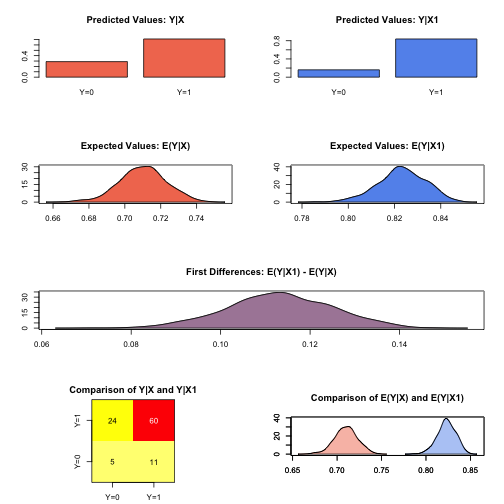
\includegraphics{Zelig-lognorm-1.png}
\caption{Zelig-lognorm}\end{figure}


\subsection{Model}
\label{vignette:id15}
Let \(Y_i^*\) be the survival time for observation \(i\) with
the density function \(f(y)\) and the corresponding distribution
function \(F(t)=\int_{0}^t f(y) dy\). This variable might be
censored for some observations at a fixed time \(y_c\) such that the
fully observed dependent variable, \(Y_i\), is defined as
\begin{gather}
\begin{split}Y_i = \left\{ \begin{array}{ll}
      Y_i^* & \textrm{if }Y_i^* \leq y_c \\
      y_c & \textrm{if }Y_i^* > y_c \\
    \end{array} \right.\end{split}\notag
\end{gather}\begin{itemize}
\item {} 
The \emph{stochastic component} is described by the distribution of the
partially observed variable, \(Y^*\). For the lognormal model,
there are two equivalent representations:
\begin{gather}
\begin{split}\begin{aligned}
    Y_i^* \; \sim \; \textrm{LogNormal}(\mu_i, \sigma^2) & \textrm{ or
} & \log(Y_i^*) \; \sim \; \textrm{Normal}(\mu_i, \sigma^2)\end{aligned}\end{split}\notag
\end{gather}
where the parameters \(\mu_i\) and \(\sigma^2\) are the mean
and variance of the Normal distribution. (Note that the output from
zelig() parameterizes scale:math:{}` = sigma{}`.)

In addition, survival models like the lognormal have three additional
properties. The hazard function \(h(t)\) measures the probability
of not surviving past time \(t\) given survival up to \(t\).
In general, the hazard function is equal to \(f(t)/S(t)\) where
the survival function \(S(t) =1 - \int_{0}^t f(s) ds\) represents the fraction still surviving at
time \(t\). The cumulative hazard function \(H(t)\) describes
the probability of dying before time \(t\). In general,
\(H(t)=
\int_{0}^{t} h(s) ds = -\log S(t)\). In the case of the lognormal
model,
\begin{gather}
\begin{split}\begin{aligned}
h(t) &=& \frac{1}{\sqrt{2 \pi} \, \sigma t \, S(t)}
\exp\left\{-\frac{1}{2 \sigma^2} (\log \lambda t)^2\right\} \\
S(t) &=& 1 - \Phi\left(\frac{1}{\sigma} \log \lambda t\right) \\
H(t) &=& -\log \left\{ 1 - \Phi\left(\frac{1}{\sigma} \log \lambda t\right) \right\}\end{aligned}\end{split}\notag
\end{gather}
where \(\Phi(\cdot)\) is the cumulative density function for the
Normal distribution.

\item {} 
The \emph{systematic component} is described as:
\begin{gather}
\begin{split}\mu_i = x_i \beta .\end{split}\notag
\end{gather}
\end{itemize}


\subsection{Quantities of Interest}
\label{vignette:id16}\begin{itemize}
\item {} 
The expected values (qi\$ev) for the lognormal model are simulations
of the expected duration:
\begin{gather}
\begin{split}E(Y) =  \exp\left(\mu_i + \frac{1}{2}\sigma^2 \right),\end{split}\notag
\end{gather}
given draws of \(\beta\) and \(\sigma\) from their sampling
distributions.

\item {} 
The predicted value is a draw from the log-normal distribution given
simulations of the parameters \((\lambda_i, \sigma)\).

\item {} 
The first difference (qi\$fd) is
\begin{gather}
\begin{split}\textrm{FD} = E(Y \mid x_1) - E(Y \mid x).\end{split}\notag
\end{gather}
\item {} 
In conditional prediction models, the average expected treatment
effect (att.ev) for the treatment group is
\begin{gather}
\begin{split}\frac{1}{\sum_{i=1}^n t_i}\sum_{i:t_i=1}^n \{ Y_i(t_i=1) - E[Y_i(t_i=0)] \},\end{split}\notag
\end{gather}
where \(t_i\) is a binary explanatory variable defining the
treatment (\(t_i=1\)) and control (\(t_i=0\)) groups. When
\(Y_i(t_i=1)\) is censored rather than observed, we replace it
with a simulation from the model given available knowledge of the
censoring process. Variation in the simulations is due to two
factors: uncertainty in the imputation process for censored
\(y_i^*\) and uncertainty in simulating \(E[Y_i(t_i=0)]\),
the counterfactual expected value of \(Y_i\) for observations in
the treatment group, under the assumption that everything stays the
same except that the treatment indicator is switched to
\(t_i=0\).

\item {} 
In conditional prediction models, the average predicted treatment
effect (att.pr) for the treatment group is
\begin{gather}
\begin{split}\frac{1}{\sum_{i=1}^n t_i} \sum_{i:t_i=1}^n \{  Y_i(t_i=1) -
\widehat{Y_i(t_i=0)} \},\end{split}\notag
\end{gather}
where \(t_i\) is a binary explanatory variable defining the
treatment (\(t_i=1\)) and control (\(t_i=0\)) groups. When
\(Y_i(t_i=1)\) is censored rather than observed, we replace it
with a simulation from the model given available knowledge of the
censoring process. Variation in the simulations are due to two
factors: uncertainty in the imputation process for censored
\(y_i^*\) and uncertainty in simulating
\(\widehat{Y_i(t_i=0)}\), the counterfactual predicted value of
\(Y_i\) for observations in the treatment group, under the
assumption that everything stays the same except that the treatment
indicator is switched to \(t_i=0\).

\end{itemize}


\subsection{Output Values}
\label{vignette:id17}
The output of each Zelig command contains useful information which you
may view. For example, if you run
\code{z.out \textless{}- zelig(Surv(Y, C) \textasciitilde{} X, model = lognorm, data)}, then you may
examine the available information in \code{z.out} by using
\code{names(z.out)}, see the coefficients by using z.out\$coefficients, and
a default summary of information through \code{summary(z.out)}.


\subsection{See also}
\label{vignette:id18}
The exponential function is part of the survival library by by Terry
Therneau, ported to R by Thomas Lumley. Advanced users may wish to refer
to \code{help(survfit)} in the survival library.


\bigskip\hrule{}\bigskip



\section{zelig-ls}
\label{vignette:zelig-ls}\label{vignette:zls}
Least Squares Regression for Continuous Dependent Variables

Use least squares regression analysis to estimate the best linear
predictor for the specified dependent variables.


\subsection{Syntax}
\label{vignette:id19}
With reference classes:

\begin{Verbatim}[commandchars=\\\{\}]
z5 \PYG{o}{\PYGZlt{}\PYGZhy{}} zls\PYG{o}{\PYGZdl{}}new\PYG{p}{(}\PYG{p}{)}
z5\PYG{o}{\PYGZdl{}}zelig\PYG{p}{(}Y \PYG{o}{\PYGZti{}} X1 \PYG{o}{+} X \PYG{o}{\PYGZti{}} X\PYG{p}{,} data \PYG{o}{=} mydata\PYG{p}{)}
z5\PYG{o}{\PYGZdl{}}setx\PYG{p}{(}\PYG{p}{)}
z5\PYG{o}{\PYGZdl{}}sim\PYG{p}{(}\PYG{p}{)}
\end{Verbatim}

With the Zelig 4 compatibility wrappers:

\begin{Verbatim}[commandchars=\\\{\}]
z.out \PYG{o}{\PYGZlt{}\PYGZhy{}} zelig\PYG{p}{(}Y \PYG{o}{\PYGZti{}} X1 \PYG{o}{+} X2\PYG{p}{,} model \PYG{o}{=} \PYG{l+s}{\PYGZdq{}}\PYG{l+s}{ls\PYGZdq{}}\PYG{p}{,} data \PYG{o}{=} mydata\PYG{p}{)}
x.out \PYG{o}{\PYGZlt{}\PYGZhy{}} setx\PYG{p}{(}z.out\PYG{p}{)}
s.out \PYG{o}{\PYGZlt{}\PYGZhy{}} sim\PYG{p}{(}z.out\PYG{p}{,} x \PYG{o}{=} x.out\PYG{p}{)}
\end{Verbatim}


\subsection{Examples}
\label{vignette:id20}

\subsubsection{Basic Example with First Differences}
\label{vignette:basic-example-with-first-differences}
Attach sample data:

\begin{Verbatim}[commandchars=\\\{\}]
data\PYG{p}{(}macro\PYG{p}{)}
\end{Verbatim}

Estimate model:

\begin{Verbatim}[commandchars=\\\{\}]
z.out1 \PYG{o}{\PYGZlt{}\PYGZhy{}} zelig\PYG{p}{(}unem \PYG{o}{\PYGZti{}} gdp \PYG{o}{+} capmob \PYG{o}{+} trade\PYG{p}{,} model \PYG{o}{=} \PYG{l+s}{\PYGZdq{}}\PYG{l+s}{ls\PYGZdq{}}\PYG{p}{,} data \PYG{o}{=} macro\PYG{p}{)}
\end{Verbatim}

\begin{Verbatim}[commandchars=\\\{\}]
\PYG{c}{\PYGZsh{}\PYGZsh{} How to cite this model in Zelig:}
\PYG{c}{\PYGZsh{}\PYGZsh{}   Kosuke Imai, Gary King, and Olivia Lau. 2007.}
\PYG{c}{\PYGZsh{}\PYGZsh{}   ls: Least Squares Regression for Continuous Dependent Variables}
\PYG{c}{\PYGZsh{}\PYGZsh{}   in Kosuke Imai, Gary King, and Olivia Lau, \PYGZdq{}Zelig: Everyone\PYGZsq{}s Statistical Software,\PYGZdq{}}
\PYG{c}{\PYGZsh{}\PYGZsh{}   http://zeligproject.org/}
\end{Verbatim}

Summarize regression coefficients:

\begin{Verbatim}[commandchars=\\\{\}]
summary\PYG{p}{(}z.out1\PYG{p}{)}
\end{Verbatim}

\begin{Verbatim}[commandchars=\\\{\}]
\PYG{c}{\PYGZsh{}\PYGZsh{} Model:}
\PYG{c}{\PYGZsh{}\PYGZsh{} \PYGZdl{}by}
\PYG{c}{\PYGZsh{}\PYGZsh{} [1] 1}
\PYG{c}{\PYGZsh{}\PYGZsh{}}
\PYG{c}{\PYGZsh{}\PYGZsh{}}
\PYG{c}{\PYGZsh{}\PYGZsh{} Call:}
\PYG{c}{\PYGZsh{}\PYGZsh{} stats::lm(formula = unem \PYGZti{} gdp + capmob + trade, data = .)}
\PYG{c}{\PYGZsh{}\PYGZsh{}}
\PYG{c}{\PYGZsh{}\PYGZsh{} Coefficients:}
\PYG{c}{\PYGZsh{}\PYGZsh{} (Intercept)          gdp       capmob        trade}
\PYG{c}{\PYGZsh{}\PYGZsh{}     6.18129     \PYGZhy{}0.32360      1.42194      0.01985}
\PYG{c}{\PYGZsh{}\PYGZsh{}}
\PYG{c}{\PYGZsh{}\PYGZsh{} Next step: Use \PYGZsq{}setx\PYGZsq{} method}
\end{Verbatim}

Set explanatory variables to their default (mean/mode) values, with
high (80th percentile) and low (20th percentile) values for the trade
variable:

\begin{Verbatim}[commandchars=\\\{\}]
x.high \PYG{o}{\PYGZlt{}\PYGZhy{}} setx\PYG{p}{(}z.out1\PYG{p}{,} trade \PYG{o}{=} quantile\PYG{p}{(}macro\PYG{o}{\PYGZdl{}}trade\PYG{p}{,} \PYG{l+m}{0.8}\PYG{p}{)}\PYG{p}{)}
x.low \PYG{o}{\PYGZlt{}\PYGZhy{}} setx\PYG{p}{(}z.out1\PYG{p}{,} trade \PYG{o}{=} quantile\PYG{p}{(}macro\PYG{o}{\PYGZdl{}}trade\PYG{p}{,} \PYG{l+m}{0.2}\PYG{p}{)}\PYG{p}{)}
\end{Verbatim}

Generate first differences for the effect of high versus low trade on GDP:

\begin{Verbatim}[commandchars=\\\{\}]
s.out1 \PYG{o}{\PYGZlt{}\PYGZhy{}} sim\PYG{p}{(}z.out1\PYG{p}{,} x \PYG{o}{=} x.high\PYG{p}{,} x1 \PYG{o}{=} x.low\PYG{p}{)}
\end{Verbatim}

\begin{Verbatim}[commandchars=\\\{\}]
summary\PYG{p}{(}s.out1\PYG{p}{)}
\end{Verbatim}

\begin{Verbatim}[commandchars=\\\{\}]
\PYG{c}{\PYGZsh{}\PYGZsh{}}
\PYG{c}{\PYGZsh{}\PYGZsh{}  sim x :}
\PYG{c}{\PYGZsh{}\PYGZsh{}  \PYGZhy{}\PYGZhy{}\PYGZhy{}\PYGZhy{}\PYGZhy{}}
\PYG{c}{\PYGZsh{}\PYGZsh{} ev}
\PYG{c}{\PYGZsh{}\PYGZsh{}       mean        sd      50\PYGZpc{}     2.5\PYGZpc{}    97.5\PYGZpc{}}
\PYG{c}{\PYGZsh{}\PYGZsh{} 1 5.430307 0.1971789 5.431243 5.038718 5.815665}
\PYG{c}{\PYGZsh{}\PYGZsh{} pv}
\PYG{c}{\PYGZsh{}\PYGZsh{}       mean        sd      50\PYGZpc{}     2.5\PYGZpc{}    97.5\PYGZpc{}}
\PYG{c}{\PYGZsh{}\PYGZsh{} 1 5.430307 0.1971789 5.431243 5.038718 5.815665}
\PYG{c}{\PYGZsh{}\PYGZsh{}}
\PYG{c}{\PYGZsh{}\PYGZsh{}  sim x1 :}
\PYG{c}{\PYGZsh{}\PYGZsh{}  \PYGZhy{}\PYGZhy{}\PYGZhy{}\PYGZhy{}\PYGZhy{}}
\PYG{c}{\PYGZsh{}\PYGZsh{} ev}
\PYG{c}{\PYGZsh{}\PYGZsh{}       mean        sd      50\PYGZpc{}    2.5\PYGZpc{}    97.5\PYGZpc{}}
\PYG{c}{\PYGZsh{}\PYGZsh{} 1 4.602931 0.1804596 4.604509 4.23388 4.957203}
\PYG{c}{\PYGZsh{}\PYGZsh{} pv}
\PYG{c}{\PYGZsh{}\PYGZsh{}       mean        sd      50\PYGZpc{}    2.5\PYGZpc{}    97.5\PYGZpc{}}
\PYG{c}{\PYGZsh{}\PYGZsh{} 1 4.602931 0.1804596 4.604509 4.23388 4.957203}
\PYG{c}{\PYGZsh{}\PYGZsh{} fd}
\PYG{c}{\PYGZsh{}\PYGZsh{}         mean        sd        50\PYGZpc{}      2.5\PYGZpc{}      97.5\PYGZpc{}}
\PYG{c}{\PYGZsh{}\PYGZsh{} 1 \PYGZhy{}0.8273756 0.2379988 \PYGZhy{}0.8281937 \PYGZhy{}1.295583 \PYGZhy{}0.3443534}
\end{Verbatim}

\begin{Verbatim}[commandchars=\\\{\}]
plot\PYG{p}{(}s.out1\PYG{p}{)}
\end{Verbatim}
\begin{figure}[htbp]
\centering

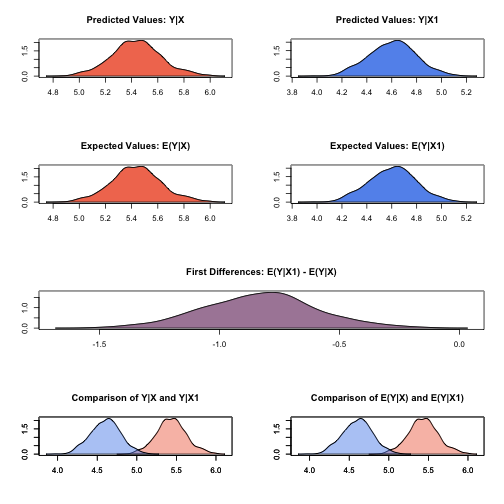
\includegraphics{unnamed-chunk-10-1.png}
\end{figure}


\subsubsection{Using Dummy Variables}
\label{vignette:using-dummy-variables}
Estimate a model with fixed effects for each country (see for help
with dummy variables). Note that you do not need to create dummy
variables, as the program will automatically parse the unique values
in the selected variable into discrete levels.

\begin{Verbatim}[commandchars=\\\{\}]
z.out2 \PYG{o}{\PYGZlt{}\PYGZhy{}} zelig\PYG{p}{(}unem \PYG{o}{\PYGZti{}} gdp \PYG{o}{+} trade \PYG{o}{+} capmob \PYG{o}{+} as.factor\PYG{p}{(}country\PYG{p}{)}\PYG{p}{,} model \PYG{o}{=} \PYG{l+s}{\PYGZdq{}}\PYG{l+s}{ls\PYGZdq{}}\PYG{p}{,} data \PYG{o}{=} macro\PYG{p}{)}
\end{Verbatim}

\begin{Verbatim}[commandchars=\\\{\}]
\PYG{c}{\PYGZsh{}\PYGZsh{} How to cite this model in Zelig:}
\PYG{c}{\PYGZsh{}\PYGZsh{}   Kosuke Imai, Gary King, and Olivia Lau. 2007.}
\PYG{c}{\PYGZsh{}\PYGZsh{}   ls: Least Squares Regression for Continuous Dependent Variables}
\PYG{c}{\PYGZsh{}\PYGZsh{}   in Kosuke Imai, Gary King, and Olivia Lau, \PYGZdq{}Zelig: Everyone\PYGZsq{}s Statistical Software,\PYGZdq{}}
\PYG{c}{\PYGZsh{}\PYGZsh{}   http://zeligproject.org/}
\end{Verbatim}

Set values for the explanatory variables, using the default mean/mode
values, with country set to the United States and Japan,
respectively:

\begin{Verbatim}[commandchars=\\\{\}]
x.US \PYG{o}{\PYGZlt{}\PYGZhy{}} setx\PYG{p}{(}z.out2\PYG{p}{,} country \PYG{o}{=} \PYG{l+s}{\PYGZdq{}}\PYG{l+s}{United States\PYGZdq{}}\PYG{p}{)}
x.Japan \PYG{o}{\PYGZlt{}\PYGZhy{}} setx\PYG{p}{(}z.out2\PYG{p}{,} country \PYG{o}{=} \PYG{l+s}{\PYGZdq{}}\PYG{l+s}{Japan\PYGZdq{}}\PYG{p}{)}
\end{Verbatim}

Simulate quantities of interest:

\begin{Verbatim}[commandchars=\\\{\}]
s.out2 \PYG{o}{\PYGZlt{}\PYGZhy{}} sim\PYG{p}{(}z.out2\PYG{p}{,} x \PYG{o}{=} x.US\PYG{p}{,} x1 \PYG{o}{=} x.Japan\PYG{p}{)}
\end{Verbatim}

\begin{Verbatim}[commandchars=\\\{\}]
plot\PYG{p}{(}s.out2\PYG{p}{)}
\end{Verbatim}
\begin{figure}[htbp]
\centering

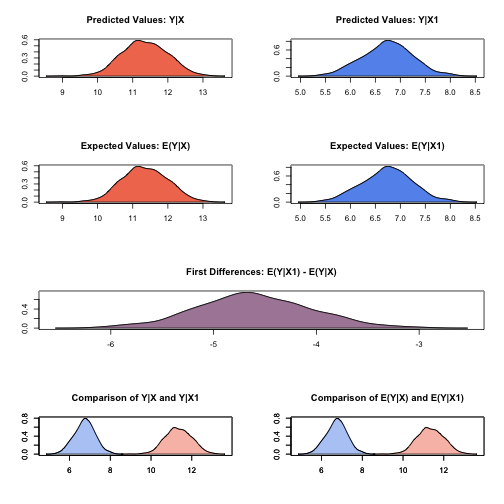
\includegraphics{unnamed-chunk-14-1.png}
\end{figure}


\subsection{Model}
\label{vignette:id21}\begin{itemize}
\item {} 
The \emph{stochastic component} is described by a density with mean
\(\mu_i\) and the common variance \(\sigma^2\)
\begin{gather}
\begin{split}Y_i \; \sim \; f(y_i \mid \mu_i, \sigma^2).\end{split}\notag
\end{gather}
\item {} 
The \emph{systematic component} models the conditional mean as
\begin{gather}
\begin{split}\mu_i =  x_i \beta\end{split}\notag
\end{gather}
where \(x_i\) is the vector of covariates, and \(\beta\) is
the vector of coefficients.

The least squares estimator is the best linear predictor of a
dependent variable given \(x_i\), and minimizes the sum of
squared residuals, \(\sum_{i=1}^n (Y_i-x_i \beta)^2\).

\end{itemize}


\subsection{Quantities of Interest}
\label{vignette:id22}\begin{itemize}
\item {} 
The expected value (qi\$ev) is the mean of simulations from the
stochastic component,
\begin{gather}
\begin{split}E(Y) = x_i \beta,\end{split}\notag
\end{gather}
given a draw of \(\beta\) from its sampling distribution.

\item {} 
In conditional prediction models, the average expected treatment
effect (att.ev) for the treatment group is
\begin{gather}
\begin{split}\frac{1}{\sum_{i=1}^n t_i}\sum_{i:t_i=1}^n \left\{ Y_i(t_i=1) -
      E[Y_i(t_i=0)] \right\},\end{split}\notag
\end{gather}
where \(t_i\) is a binary explanatory variable defining the
treatment (\(t_i=1\)) and control (\(t_i=0\)) groups.
Variation in the simulations are due to uncertainty in simulating
\(E[Y_i(t_i=0)]\), the counterfactual expected value of
\(Y_i\) for observations in the treatment group, under the
assumption that everything stays the same except that the treatment
indicator is switched to \(t_i=0\).

\end{itemize}


\subsection{Output Values}
\label{vignette:id23}
The output of each Zelig command contains useful information which you
may view. For example, if you run
\code{z.out \textless{}- zelig(y \textasciitilde{} x, model = ls, data)}, then you may examine the
available information in \code{z.out} by using \code{names(z.out)}, see the
coefficients by using z.out\$coefficients, and a default summary of
information through \code{summary(z.out)}. Other elements available through
the \$ operator are listed below.
\begin{itemize}
\item {} 
From the zelig() output object z.out, you may extract:
\begin{itemize}
\item {} 
coefficients: parameter estimates for the explanatory variables.

\item {} 
residuals: the working residuals in the final iteration of the
IWLS fit.

\item {} 
fitted.values: fitted values.

\item {} 
df.residual: the residual degrees of freedom.

\item {} 
zelig.data: the input data frame if save.data = TRUE.

\end{itemize}

\item {} 
From summary(z.out), you may extract:
\begin{itemize}
\item {} 
coefficients: the parameter estimates with their associated
standard errors, \(p\)-values, and \(t\)-statistics.
\begin{gather}
\begin{split}\hat{\beta} \; = \; \left(\sum_{i=1}^n x_i' x_i\right)^{-1} \sum x_i y_i\end{split}\notag
\end{gather}
\item {} 
sigma: the square root of the estimate variance of the random
error \(e\):
\begin{gather}
\begin{split}\hat{\sigma} \; = \; \frac{\sum (Y_i-x_i\hat{\beta})^2}{n-k}\end{split}\notag
\end{gather}
\item {} 
r.squared: the fraction of the variance explained by the model.
\begin{gather}
\begin{split}R^2 \; = \; 1 - \frac{\sum (Y_i-x_i\hat{\beta})^2}{\sum (y_i -
         \bar{y})^2}\end{split}\notag
\end{gather}
\item {} 
adj.r.squared: the above \(R^2\) statistic, penalizing for an
increased number of explanatory variables.

\item {} 
cov.unscaled: a \(k \times k\) matrix of unscaled covariances.

\end{itemize}

\end{itemize}


\subsection{See also}
\label{vignette:id24}
The least squares regression is part of the stats package by William N.
Venables and Brian D. Ripley .In addition, advanced users may wish to
refer to \code{help(lm)} and \code{help(lm.fit)}.


\bigskip\hrule{}\bigskip



\section{zelig-negbin}
\label{vignette:znegbin}\label{vignette:zelig-negbin}
Negative Binomial Regression for Event Count Dependent Variables

Use the negative binomial regression if you have a count of events for
each observation of your dependent variable. The negative binomial model
is frequently used to estimate over-dispersed event count models.


\subsection{Syntax}
\label{vignette:id25}
With reference classes:

\begin{Verbatim}[commandchars=\\\{\}]
z5 \PYG{o}{\PYGZlt{}\PYGZhy{}} znegbin\PYG{o}{\PYGZdl{}}new\PYG{p}{(}\PYG{p}{)}
z5\PYG{o}{\PYGZdl{}}zelig\PYG{p}{(}Y \PYG{o}{\PYGZti{}} X1 \PYG{o}{+} X \PYG{o}{\PYGZti{}} X\PYG{p}{,} data \PYG{o}{=} mydata\PYG{p}{)}
z5\PYG{o}{\PYGZdl{}}setx\PYG{p}{(}\PYG{p}{)}
z5\PYG{o}{\PYGZdl{}}sim\PYG{p}{(}\PYG{p}{)}
\end{Verbatim}

With the Zelig 4 compatibility wrappers:

\begin{Verbatim}[commandchars=\\\{\}]
z.out \PYG{o}{\PYGZlt{}\PYGZhy{}} zelig\PYG{p}{(}Y \PYG{o}{\PYGZti{}} X1 \PYG{o}{+} X2\PYG{p}{,} model \PYG{o}{=} \PYG{l+s}{\PYGZdq{}}\PYG{l+s}{negbin\PYGZdq{}}\PYG{p}{,} data \PYG{o}{=} mydata\PYG{p}{)}
x.out \PYG{o}{\PYGZlt{}\PYGZhy{}} setx\PYG{p}{(}z.out\PYG{p}{)}
s.out \PYG{o}{\PYGZlt{}\PYGZhy{}} sim\PYG{p}{(}z.out\PYG{p}{,} x \PYG{o}{=} x.out\PYG{p}{)}
\end{Verbatim}


\subsection{Example}
\label{vignette:id26}
Load sample data:

\begin{Verbatim}[commandchars=\\\{\}]
data\PYG{p}{(}sanction\PYG{p}{)}
\end{Verbatim}

Estimate the model:

\begin{Verbatim}[commandchars=\\\{\}]
z.out \PYG{o}{\PYGZlt{}\PYGZhy{}} zelig\PYG{p}{(}num \PYG{o}{\PYGZti{}} target \PYG{o}{+} coop\PYG{p}{,} model \PYG{o}{=} \PYG{l+s}{\PYGZdq{}}\PYG{l+s}{negbin\PYGZdq{}}\PYG{p}{,} data \PYG{o}{=} sanction\PYG{p}{)}
\end{Verbatim}

\begin{Verbatim}[commandchars=\\\{\}]
\PYG{c}{\PYGZsh{}\PYGZsh{} How to cite this model in Zelig:}
\PYG{c}{\PYGZsh{}\PYGZsh{}   Kosuke Imai, Gary King, Olivia Lau. 2008.}
\PYG{c}{\PYGZsh{}\PYGZsh{}   negbinom: Negative Binomial Regression for Event Count Dependent Variables}
\PYG{c}{\PYGZsh{}\PYGZsh{}   in Kosuke Imai, Gary King, and Olivia Lau, \PYGZdq{}Zelig: Everyone\PYGZsq{}s Statistical Software,\PYGZdq{}}
\PYG{c}{\PYGZsh{}\PYGZsh{}   http://zeligproject.org/}
\end{Verbatim}

\begin{Verbatim}[commandchars=\\\{\}]
summary\PYG{p}{(}z.out\PYG{p}{)}
\end{Verbatim}

\begin{Verbatim}[commandchars=\\\{\}]
\PYG{c}{\PYGZsh{}\PYGZsh{} Model:}
\PYG{c}{\PYGZsh{}\PYGZsh{} \PYGZdl{}by}
\PYG{c}{\PYGZsh{}\PYGZsh{} [1] 1}
\PYG{c}{\PYGZsh{}\PYGZsh{}}
\PYG{c}{\PYGZsh{}\PYGZsh{}}
\PYG{c}{\PYGZsh{}\PYGZsh{} Call:  MASS::glm.nb(formula = num \PYGZti{} target + coop, data = ., init.theta = 1.841603403,}
\PYG{c}{\PYGZsh{}\PYGZsh{}     link = log)}
\PYG{c}{\PYGZsh{}\PYGZsh{}}
\PYG{c}{\PYGZsh{}\PYGZsh{} Coefficients:}
\PYG{c}{\PYGZsh{}\PYGZsh{} (Intercept)       target         coop}
\PYG{c}{\PYGZsh{}\PYGZsh{}      \PYGZhy{}1.564        0.151        1.286}
\PYG{c}{\PYGZsh{}\PYGZsh{}}
\PYG{c}{\PYGZsh{}\PYGZsh{} Degrees of Freedom: 77 Total (i.e. Null);  75 Residual}
\PYG{c}{\PYGZsh{}\PYGZsh{} Null Deviance:       237.1}
\PYG{c}{\PYGZsh{}\PYGZsh{} Residual Deviance: 56.55         AIC: 360.2}
\PYG{c}{\PYGZsh{}\PYGZsh{} Next step: Use \PYGZsq{}setx\PYGZsq{} method}
\end{Verbatim}

Set values for the explanatory variables to their default mean values:

\begin{Verbatim}[commandchars=\\\{\}]
x.out \PYG{o}{\PYGZlt{}\PYGZhy{}} setx\PYG{p}{(}z.out\PYG{p}{)}
\end{Verbatim}

Simulate fitted values:

\begin{Verbatim}[commandchars=\\\{\}]
s.out \PYG{o}{\PYGZlt{}\PYGZhy{}} sim\PYG{p}{(}z.out\PYG{p}{,} x \PYG{o}{=} x.out\PYG{p}{)}
\end{Verbatim}

\begin{Verbatim}[commandchars=\\\{\}]
summary\PYG{p}{(}s.out\PYG{p}{)}
\end{Verbatim}

\begin{Verbatim}[commandchars=\\\{\}]
\PYG{c}{\PYGZsh{}\PYGZsh{}}
\PYG{c}{\PYGZsh{}\PYGZsh{}  sim x :}
\PYG{c}{\PYGZsh{}\PYGZsh{}  \PYGZhy{}\PYGZhy{}\PYGZhy{}\PYGZhy{}\PYGZhy{}}
\PYG{c}{\PYGZsh{}\PYGZsh{} ev}
\PYG{c}{\PYGZsh{}\PYGZsh{}          mean       sd      50\PYGZpc{}     2.5\PYGZpc{}    97.5\PYGZpc{}}
\PYG{c}{\PYGZsh{}\PYGZsh{} [1,] 2.948528 0.360773 2.916141 2.323829 3.703429}
\PYG{c}{\PYGZsh{}\PYGZsh{} pv}
\PYG{c}{\PYGZsh{}\PYGZsh{} qi}
\PYG{c}{\PYGZsh{}\PYGZsh{}     0     1     2     3     4     5     6     7     8     9    10    11}
\PYG{c}{\PYGZsh{}\PYGZsh{} 0.193 0.189 0.186 0.134 0.095 0.064 0.045 0.036 0.026 0.007 0.007 0.009}
\PYG{c}{\PYGZsh{}\PYGZsh{}    12    13    14    15    16    17    30}
\PYG{c}{\PYGZsh{}\PYGZsh{} 0.002 0.001 0.001 0.002 0.001 0.001 0.001}
\end{Verbatim}

\begin{Verbatim}[commandchars=\\\{\}]
plot\PYG{p}{(}s.out\PYG{p}{)}
\end{Verbatim}
\begin{figure}[htbp]
\centering
\capstart

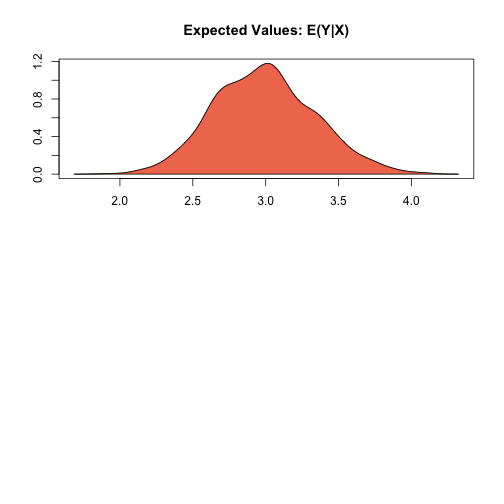
\includegraphics{Zelig-negbin-1.png}
\caption{Zelig-negbin}\end{figure}


\subsection{Model}
\label{vignette:id27}
Let \(Y_i\) be the number of independent events that occur during a
fixed time period. This variable can take any non-negative integer
value.
\begin{itemize}
\item {} 
The negative binomial distribution is derived by letting the mean of
the Poisson distribution vary according to a fixed parameter
\(\zeta\) given by the Gamma distribution. The \emph{stochastic
component} is given by
\begin{gather}
\begin{split}\begin{aligned}
     Y_i \mid \zeta_i & \sim & \textrm{Poisson}(\zeta_i \mu_i),\\
     \zeta_i & \sim & \frac{1}{\theta}\textrm{Gamma}(\theta).
   \end{aligned}\end{split}\notag
\end{gather}
The marginal distribution of \(Y_i\) is then the negative
binomial with mean \(\mu_i\) and variance
\(\mu_i + \mu_i^2/\theta\):
\begin{gather}
\begin{split}\begin{aligned}
   Y_i & \sim & \textrm{NegBin}(\mu_i, \theta), \\
       & = & \frac{\Gamma (\theta + y_i)}{y! \, \Gamma(\theta)}
             \frac{\mu_i^{y_i} \, \theta^{\theta}}{(\mu_i + \theta)^{\theta + y_i}},
   \end{aligned}\end{split}\notag
\end{gather}
where \(\theta\) is the systematic parameter of the Gamma
distribution modeling \(\zeta_i\).

\item {} 
The \emph{systematic component} is given by
\begin{gather}
\begin{split}\mu_i = \exp(x_i \beta)\end{split}\notag
\end{gather}
where \(x_i\) is the vector of \(k\) explanatory variables
and \(\beta\) is the vector of coefficients.

\end{itemize}


\subsection{Quantities of Interest}
\label{vignette:id28}\begin{itemize}
\item {} 
The expected values (qi\$ev) are simulations of the mean of the
stochastic component. Thus,
\begin{gather}
\begin{split}E(Y) = \mu_i = \exp(x_i
  \beta),\end{split}\notag
\end{gather}
given simulations of \(\beta\).

\item {} 
The predicted value (qi\$pr) drawn from the distribution defined by
the set of parameters \((\mu_i, \theta)\).

\item {} 
The first difference (qi\$fd) is
\begin{gather}
\begin{split}\textrm{FD} \; = \; E(Y | x_1) - E(Y \mid x)\end{split}\notag
\end{gather}
\item {} 
In conditional prediction models, the average expected treatment
effect (att.ev) for the treatment group is
\begin{gather}
\begin{split}\frac{1}{\sum_{i=1}^n t_i}\sum_{i:t_i=1}^n \left\{ Y_i(t_i=1) -
      E[Y_i(t_i=0)] \right\},\end{split}\notag
\end{gather}
where \(t_i\) is a binary explanatory variable defining the
treatment (\(t_i=1\)) and control (\(t_i=0\)) groups.
Variation in the simulations are due to uncertainty in simulating
\(E[Y_i(t_i=0)]\), the counterfactual expected value of
\(Y_i\) for observations in the treatment group, under the
assumption that everything stays the same except that the treatment
indicator is switched to \(t_i=0\).

\item {} 
In conditional prediction models, the average predicted treatment
effect (att.pr) for the treatment group is
\begin{gather}
\begin{split}\frac{1}{\sum_{i=1}^n t_i}\sum_{i:t_i=1}^n \left\{ Y_i(t_i=1) -
      \widehat{Y_i(t_i=0)} \right\},\end{split}\notag
\end{gather}
where \(t_i\) is a binary explanatory variable defining the
treatment (\(t_i=1\)) and control (\(t_i=0\)) groups.
Variation in the simulations are due to uncertainty in simulating
\(\widehat{Y_i(t_i=0)}\), the counterfactual predicted value of
\(Y_i\) for observations in the treatment group, under the
assumption that everything stays the same except that the treatment
indicator is switched to \(t_i=0\).

\end{itemize}


\subsection{Output Values}
\label{vignette:id29}
The output of each Zelig command contains useful information which you
may view. For example, if you run
\code{z.out \textless{}- zelig(y \textasciitilde{} x, model = negbin, data)}, then you may examine
the available information in \code{z.out} by using \code{names(z.out)}, see
the coefficients by using z.out\$coefficients, and a default summary of
information through \code{summary(z.out)}.


\subsection{See also}
\label{vignette:id30}
The negative binomial model is part of the MASS package by William N.
Venable and Brian D. Ripley . Advanced users may wish to refer to
{\color{red}\bfseries{}{}`{}`}help(glm.nb){}`.


\bigskip\hrule{}\bigskip



\section{zelig-normal}
\label{vignette:zelig-normal}\label{vignette:znorm}
Normal Regression for Continuous Dependent Variables

The Normal regression model is a close variant of the more standard
least squares regression model (see ). Both models specify a continuous
dependent variable as a linear function of a set of explanatory
variables. The Normal model reports maximum likelihood (rather than
least squares) estimates. The two models differ only in their estimate
for the stochastic parameter \(\sigma\).


\subsection{Syntax}
\label{vignette:id33}
With reference classes:

\begin{Verbatim}[commandchars=\\\{\}]
z5 \PYG{o}{\PYGZlt{}\PYGZhy{}} znormal\PYG{o}{\PYGZdl{}}new\PYG{p}{(}\PYG{p}{)}
z5\PYG{o}{\PYGZdl{}}zelig\PYG{p}{(}Y \PYG{o}{\PYGZti{}} X1 \PYG{o}{+} X \PYG{o}{\PYGZti{}} X\PYG{p}{,} data \PYG{o}{=} mydata\PYG{p}{)}
z5\PYG{o}{\PYGZdl{}}setx\PYG{p}{(}\PYG{p}{)}
z5\PYG{o}{\PYGZdl{}}sim\PYG{p}{(}\PYG{p}{)}
\end{Verbatim}

With the Zelig 4 compatibility wrappers:

\begin{Verbatim}[commandchars=\\\{\}]
z.out \PYG{o}{\PYGZlt{}\PYGZhy{}} zelig\PYG{p}{(}Y \PYG{o}{\PYGZti{}} X1 \PYG{o}{+} X2\PYG{p}{,} model \PYG{o}{=} \PYG{l+s}{\PYGZdq{}}\PYG{l+s}{normal\PYGZdq{}}\PYG{p}{,} data \PYG{o}{=} mydata\PYG{p}{)}
x.out \PYG{o}{\PYGZlt{}\PYGZhy{}} setx\PYG{p}{(}z.out\PYG{p}{)}
s.out \PYG{o}{\PYGZlt{}\PYGZhy{}} sim\PYG{p}{(}z.out\PYG{p}{,} x \PYG{o}{=} x.out\PYG{p}{)}
\end{Verbatim}


\subsection{Examples}
\label{vignette:id34}

\subsubsection{Basic Example with First Differences}
\label{vignette:id35}
Attach sample data:

\begin{Verbatim}[commandchars=\\\{\}]
data\PYG{p}{(}macro\PYG{p}{)}
\end{Verbatim}

Estimate model:

\begin{Verbatim}[commandchars=\\\{\}]
z.out1 \PYG{o}{\PYGZlt{}\PYGZhy{}} zelig\PYG{p}{(}unem \PYG{o}{\PYGZti{}} gdp \PYG{o}{+} capmob \PYG{o}{+} trade\PYG{p}{,} model \PYG{o}{=} \PYG{l+s}{\PYGZdq{}}\PYG{l+s}{normal\PYGZdq{}}\PYG{p}{,} data \PYG{o}{=} macro\PYG{p}{)}
\end{Verbatim}

\begin{Verbatim}[commandchars=\\\{\}]
\PYG{c}{\PYGZsh{}\PYGZsh{} How to cite this model in Zelig:}
\PYG{c}{\PYGZsh{}\PYGZsh{}   Kosuke Imai, Gary King, Olivia Lau. 2008.}
\PYG{c}{\PYGZsh{}\PYGZsh{}   normal: Normal Regression for Continuous Dependent Variables}
\PYG{c}{\PYGZsh{}\PYGZsh{}   in Kosuke Imai, Gary King, and Olivia Lau, \PYGZdq{}Zelig: Everyone\PYGZsq{}s Statistical Software,\PYGZdq{}}
\PYG{c}{\PYGZsh{}\PYGZsh{}   http://zeligproject.org/}
\end{Verbatim}

Summarize of regression coefficients:

\begin{Verbatim}[commandchars=\\\{\}]
summary\PYG{p}{(}z.out1\PYG{p}{)}
\end{Verbatim}

\begin{Verbatim}[commandchars=\\\{\}]
\PYG{c}{\PYGZsh{}\PYGZsh{} Model:}
\PYG{c}{\PYGZsh{}\PYGZsh{} \PYGZdl{}by}
\PYG{c}{\PYGZsh{}\PYGZsh{} [1] 1}
\PYG{c}{\PYGZsh{}\PYGZsh{}}
\PYG{c}{\PYGZsh{}\PYGZsh{}}
\PYG{c}{\PYGZsh{}\PYGZsh{} Call:  stats::glm(formula = unem \PYGZti{} gdp + capmob + trade, family = gaussian(\PYGZdq{}identity\PYGZdq{}),}
\PYG{c}{\PYGZsh{}\PYGZsh{}     data = .)}
\PYG{c}{\PYGZsh{}\PYGZsh{}}
\PYG{c}{\PYGZsh{}\PYGZsh{} Coefficients:}
\PYG{c}{\PYGZsh{}\PYGZsh{} (Intercept)          gdp       capmob        trade}
\PYG{c}{\PYGZsh{}\PYGZsh{}     6.18129     \PYGZhy{}0.32360      1.42194      0.01985}
\PYG{c}{\PYGZsh{}\PYGZsh{}}
\PYG{c}{\PYGZsh{}\PYGZsh{} Degrees of Freedom: 349 Total (i.e. Null);  346 Residual}
\PYG{c}{\PYGZsh{}\PYGZsh{} Null Deviance:       3665}
\PYG{c}{\PYGZsh{}\PYGZsh{} Residual Deviance: 2610  AIC: 1706}
\PYG{c}{\PYGZsh{}\PYGZsh{} Next step: Use \PYGZsq{}setx\PYGZsq{} method}
\end{Verbatim}

Set explanatory variables to their default (mean/mode) values, with
high (80th percentile) and low (20th percentile) values for trade:

\begin{Verbatim}[commandchars=\\\{\}]
x.high \PYG{o}{\PYGZlt{}\PYGZhy{}} setx\PYG{p}{(}z.out1\PYG{p}{,} trade \PYG{o}{=} quantile\PYG{p}{(}macro\PYG{o}{\PYGZdl{}}trade\PYG{p}{,} \PYG{l+m}{0.8}\PYG{p}{)}\PYG{p}{)}
x.low \PYG{o}{\PYGZlt{}\PYGZhy{}} setx\PYG{p}{(}z.out1\PYG{p}{,} trade \PYG{o}{=} quantile\PYG{p}{(}macro\PYG{o}{\PYGZdl{}}trade\PYG{p}{,} \PYG{l+m}{0.2}\PYG{p}{)}\PYG{p}{)}
\end{Verbatim}

Generate first differences for the effect of high versus low trade on GDP:

\begin{Verbatim}[commandchars=\\\{\}]
s.out1 \PYG{o}{\PYGZlt{}\PYGZhy{}} sim\PYG{p}{(}z.out1\PYG{p}{,} x \PYG{o}{=} x.high\PYG{p}{,} x1 \PYG{o}{=} x.low\PYG{p}{)}
\end{Verbatim}

\begin{Verbatim}[commandchars=\\\{\}]
summary\PYG{p}{(}s.out1\PYG{p}{)}
\end{Verbatim}

\begin{Verbatim}[commandchars=\\\{\}]
\PYG{c}{\PYGZsh{}\PYGZsh{}}
\PYG{c}{\PYGZsh{}\PYGZsh{}  sim x :}
\PYG{c}{\PYGZsh{}\PYGZsh{}  \PYGZhy{}\PYGZhy{}\PYGZhy{}\PYGZhy{}\PYGZhy{}}
\PYG{c}{\PYGZsh{}\PYGZsh{} ev}
\PYG{c}{\PYGZsh{}\PYGZsh{}          mean        sd      50\PYGZpc{}     2.5\PYGZpc{}    97.5\PYGZpc{}}
\PYG{c}{\PYGZsh{}\PYGZsh{} [1,] 5.433104 0.1993954 5.432221 5.032391 5.833022}
\PYG{c}{\PYGZsh{}\PYGZsh{} pv}
\PYG{c}{\PYGZsh{}\PYGZsh{}          mean       sd      50\PYGZpc{}       2.5\PYGZpc{}    97.5\PYGZpc{}}
\PYG{c}{\PYGZsh{}\PYGZsh{} [1,] 5.460641 2.736715 5.472975 0.09863579 10.62646}
\PYG{c}{\PYGZsh{}\PYGZsh{}}
\PYG{c}{\PYGZsh{}\PYGZsh{}  sim x1 :}
\PYG{c}{\PYGZsh{}\PYGZsh{}  \PYGZhy{}\PYGZhy{}\PYGZhy{}\PYGZhy{}\PYGZhy{}}
\PYG{c}{\PYGZsh{}\PYGZsh{} ev}
\PYG{c}{\PYGZsh{}\PYGZsh{}          mean        sd      50\PYGZpc{}     2.5\PYGZpc{}    97.5\PYGZpc{}}
\PYG{c}{\PYGZsh{}\PYGZsh{} [1,] 4.602042 0.1755117 4.613065 4.252265 4.945202}
\PYG{c}{\PYGZsh{}\PYGZsh{} pv}
\PYG{c}{\PYGZsh{}\PYGZsh{}          mean       sd      50\PYGZpc{}       2.5\PYGZpc{}    97.5\PYGZpc{}}
\PYG{c}{\PYGZsh{}\PYGZsh{} [1,] 4.767229 2.699091 4.677271 \PYGZhy{}0.5714166 10.08173}
\PYG{c}{\PYGZsh{}\PYGZsh{} fd}
\PYG{c}{\PYGZsh{}\PYGZsh{}           mean        sd        50\PYGZpc{}      2.5\PYGZpc{}      97.5\PYGZpc{}}
\PYG{c}{\PYGZsh{}\PYGZsh{} [1,] \PYGZhy{}0.831062 0.2364614 \PYGZhy{}0.8278868 \PYGZhy{}1.296051 \PYGZhy{}0.3667207}
\end{Verbatim}

A visual summary of quantities of interest:

\begin{Verbatim}[commandchars=\\\{\}]
plot\PYG{p}{(}s.out1\PYG{p}{)}
\end{Verbatim}
\begin{figure}[htbp]
\centering
\capstart

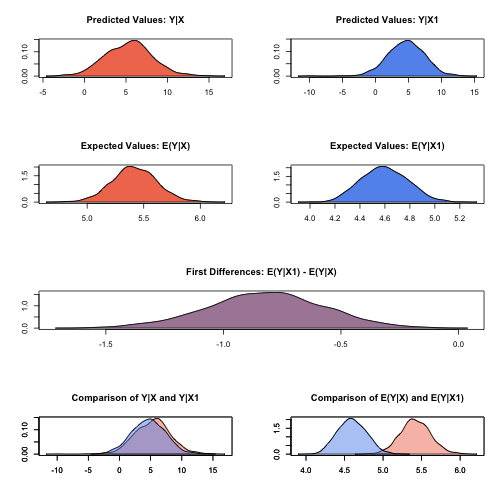
\includegraphics{Zelig-normal-1.png}
\caption{Zelig-normal}\end{figure}


\subsection{Model}
\label{vignette:id36}
Let \(Y_i\) be the continuous dependent variable for observation
\(i\).
\begin{itemize}
\item {} 
The \emph{stochastic component} is described by a univariate normal model
with a vector of means \(\mu_i\) and scalar variance
\(\sigma^2\):
\begin{gather}
\begin{split}Y_i \; \sim \; \textrm{Normal}(\mu_i, \sigma^2).\end{split}\notag
\end{gather}
\item {} 
The \emph{systematic component} is
\begin{gather}
\begin{split}\mu_i \;= \; x_i \beta,\end{split}\notag
\end{gather}
where \(x_i\) is the vector of \(k\) explanatory variables
and \(\beta\) is the vector of coefficients.

\end{itemize}


\subsection{Quantities of Interest}
\label{vignette:id37}\begin{itemize}
\item {} 
The expected value (qi\$ev) is the mean of simulations from the the
stochastic component,
\begin{gather}
\begin{split}E(Y) = \mu_i = x_i \beta,\end{split}\notag
\end{gather}
given a draw of \(\beta\) from its posterior.

\item {} 
The predicted value (qi\$pr) is drawn from the distribution defined by
the set of parameters \((\mu_i, \sigma)\).

\item {} 
The first difference (qi\$fd) is:
\begin{gather}
\begin{split}\textrm{FD}\; = \;E(Y \mid x_1) -  E(Y \mid x)\end{split}\notag
\end{gather}
\item {} 
In conditional prediction models, the average expected treatment
effect (att.ev) for the treatment group is
\begin{gather}
\begin{split}\frac{1}{\sum_{i=1}^n t_i}\sum_{i:t_i=1}^n \left\{ Y_i(t_i=1) -
      E[Y_i(t_i=0)] \right\},\end{split}\notag
\end{gather}
where \(t_i\) is a binary explanatory variable defining the
treatment (\(t_i=1\)) and control (\(t_i=0\)) groups.
Variation in the simulations are due to uncertainty in simulating
\(E[Y_i(t_i=0)]\), the counterfactual expected value of
\(Y_i\) for observations in the treatment group, under the
assumption that everything stays the same except that the treatment
indicator is switched to \(t_i=0\).

\item {} 
In conditional prediction models, the average predicted treatment
effect (att.pr) for the treatment group is
\begin{gather}
\begin{split}\frac{1}{\sum_{i=1}^n t_i}\sum_{i:t_i=1}^n \left\{ Y_i(t_i=1) -
      \widehat{Y_i(t_i=0)} \right\},\end{split}\notag
\end{gather}
where \(t_i\) is a binary explanatory variable defining the
treatment (\(t_i=1\)) and control (\(t_i=0\)) groups.
Variation in the simulations are due to uncertainty in simulating
\(\widehat{Y_i(t_i=0)}\), the counterfactual predicted value of
\(Y_i\) for observations in the treatment group, under the
assumption that everything stays the same except that the treatment
indicator is switched to \(t_i=0\).

\end{itemize}


\subsection{Output Values}
\label{vignette:id38}
The output of each Zelig command contains useful information which you
may view. For example, if you run
\code{z.out \textless{}- zelig(y \textasciitilde{} x, model = normal, data)}, then you may examine
the available information in \code{z.out} by using \code{names(z.out)}, see
the coefficients by using z.out\$coefficients, and a default summary of
information through \code{summary(z.out)}.


\subsection{See also}
\label{vignette:id39}
The normal model is part of the stats package by . Advanced users may
wish to refer to \code{help(glm)} and \code{help(family)}.


\bigskip\hrule{}\bigskip



\section{zelig-poisson}
\label{vignette:zpoisson}\label{vignette:zelig-poisson}
Poisson Regression for Event Count Dependent Variables

Use the Poisson regression model if the observations of your dependent
variable represents the number of independent events that occur during a
fixed period of time (see the negative binomial model, , for
over-dispersed event counts.) For a Bayesian implementation of this
model, see .


\subsection{Syntax}
\label{vignette:id40}
With reference classes:

\begin{Verbatim}[commandchars=\\\{\}]
z5 \PYG{o}{\PYGZlt{}\PYGZhy{}} zpoisson\PYG{o}{\PYGZdl{}}new\PYG{p}{(}\PYG{p}{)}
z5\PYG{o}{\PYGZdl{}}zelig\PYG{p}{(}Y \PYG{o}{\PYGZti{}} X1 \PYG{o}{+} X \PYG{o}{\PYGZti{}} X\PYG{p}{,} data \PYG{o}{=} mydata\PYG{p}{)}
z5\PYG{o}{\PYGZdl{}}setx\PYG{p}{(}\PYG{p}{)}
z5\PYG{o}{\PYGZdl{}}sim\PYG{p}{(}\PYG{p}{)}
\end{Verbatim}

With the Zelig 4 compatibility wrappers:

\begin{Verbatim}[commandchars=\\\{\}]
z.out \PYG{o}{\PYGZlt{}\PYGZhy{}} zelig\PYG{p}{(}Y \PYG{o}{\PYGZti{}} X1 \PYG{o}{+} X2\PYG{p}{,} model \PYG{o}{=} \PYG{l+s}{\PYGZdq{}}\PYG{l+s}{poisson\PYGZdq{}}\PYG{p}{,} data \PYG{o}{=} mydata\PYG{p}{)}
x.out \PYG{o}{\PYGZlt{}\PYGZhy{}} setx\PYG{p}{(}z.out\PYG{p}{)}
s.out \PYG{o}{\PYGZlt{}\PYGZhy{}} sim\PYG{p}{(}z.out\PYG{p}{,} x \PYG{o}{=} x.out\PYG{p}{)}
\end{Verbatim}


\subsection{Example}
\label{vignette:id41}
Load sample data:

\begin{Verbatim}[commandchars=\\\{\}]
data\PYG{p}{(}sanction\PYG{p}{)}
\end{Verbatim}

Estimate Poisson model:

\begin{Verbatim}[commandchars=\\\{\}]
z.out \PYG{o}{\PYGZlt{}\PYGZhy{}} zelig\PYG{p}{(}num \PYG{o}{\PYGZti{}} target \PYG{o}{+} coop\PYG{p}{,} model \PYG{o}{=} \PYG{l+s}{\PYGZdq{}}\PYG{l+s}{poisson\PYGZdq{}}\PYG{p}{,} data \PYG{o}{=} sanction\PYG{p}{)}
\end{Verbatim}

\begin{Verbatim}[commandchars=\\\{\}]
\PYG{c}{\PYGZsh{}\PYGZsh{} How to cite this model in Zelig:}
\PYG{c}{\PYGZsh{}\PYGZsh{}   Kosuke Imai, Gary King, Olivia Lau. 2007.}
\PYG{c}{\PYGZsh{}\PYGZsh{}   poisson: Poisson Regression for Event Count Dependent Variables}
\PYG{c}{\PYGZsh{}\PYGZsh{}   in Kosuke Imai, Gary King, and Olivia Lau, \PYGZdq{}Zelig: Everyone\PYGZsq{}s Statistical Software,\PYGZdq{}}
\PYG{c}{\PYGZsh{}\PYGZsh{}   http://zeligproject.org/}
\end{Verbatim}

\begin{Verbatim}[commandchars=\\\{\}]
summary\PYG{p}{(}z.out\PYG{p}{)}
\end{Verbatim}

\begin{Verbatim}[commandchars=\\\{\}]
\PYG{c}{\PYGZsh{}\PYGZsh{} Model:}
\PYG{c}{\PYGZsh{}\PYGZsh{} \PYGZdl{}by}
\PYG{c}{\PYGZsh{}\PYGZsh{} [1] 1}
\PYG{c}{\PYGZsh{}\PYGZsh{}}
\PYG{c}{\PYGZsh{}\PYGZsh{}}
\PYG{c}{\PYGZsh{}\PYGZsh{} Call:  stats::glm(formula = num \PYGZti{} target + coop, family = poisson(\PYGZdq{}log\PYGZdq{}),}
\PYG{c}{\PYGZsh{}\PYGZsh{}     data = .)}
\PYG{c}{\PYGZsh{}\PYGZsh{}}
\PYG{c}{\PYGZsh{}\PYGZsh{} Coefficients:}
\PYG{c}{\PYGZsh{}\PYGZsh{} (Intercept)       target         coop}
\PYG{c}{\PYGZsh{}\PYGZsh{}    \PYGZhy{}0.96772     \PYGZhy{}0.02102      1.21082}
\PYG{c}{\PYGZsh{}\PYGZsh{}}
\PYG{c}{\PYGZsh{}\PYGZsh{} Degrees of Freedom: 77 Total (i.e. Null);  75 Residual}
\PYG{c}{\PYGZsh{}\PYGZsh{} Null Deviance:       1584}
\PYG{c}{\PYGZsh{}\PYGZsh{} Residual Deviance: 720.8         AIC: 944.3}
\PYG{c}{\PYGZsh{}\PYGZsh{} Next step: Use \PYGZsq{}setx\PYGZsq{} method}
\end{Verbatim}

Set values for the explanatory variables to their default mean values:

\begin{Verbatim}[commandchars=\\\{\}]
x.out \PYG{o}{\PYGZlt{}\PYGZhy{}} setx\PYG{p}{(}z.out\PYG{p}{)}
\end{Verbatim}

Simulate fitted values:

\begin{Verbatim}[commandchars=\\\{\}]
s.out \PYG{o}{\PYGZlt{}\PYGZhy{}} sim\PYG{p}{(}z.out\PYG{p}{,} x \PYG{o}{=} x.out\PYG{p}{)}
summary\PYG{p}{(}s.out\PYG{p}{)}
\end{Verbatim}

\begin{Verbatim}[commandchars=\\\{\}]
\PYG{c}{\PYGZsh{}\PYGZsh{}}
\PYG{c}{\PYGZsh{}\PYGZsh{}  sim x :}
\PYG{c}{\PYGZsh{}\PYGZsh{}  \PYGZhy{}\PYGZhy{}\PYGZhy{}\PYGZhy{}\PYGZhy{}}
\PYG{c}{\PYGZsh{}\PYGZsh{} ev}
\PYG{c}{\PYGZsh{}\PYGZsh{}         mean        sd      50\PYGZpc{}     2.5\PYGZpc{}    97.5\PYGZpc{}}
\PYG{c}{\PYGZsh{}\PYGZsh{} [1,] 3.25377 0.2285971 3.253635 2.828186 3.714806}
\PYG{c}{\PYGZsh{}\PYGZsh{} pv}
\PYG{c}{\PYGZsh{}\PYGZsh{}       mean       sd 50\PYGZpc{} 2.5\PYGZpc{} 97.5\PYGZpc{}}
\PYG{c}{\PYGZsh{}\PYGZsh{} [1,] 3.253 1.896995   3    0     7}
\end{Verbatim}

\begin{Verbatim}[commandchars=\\\{\}]
plot\PYG{p}{(}s.out\PYG{p}{)}
\end{Verbatim}
\begin{figure}[htbp]
\centering
\capstart

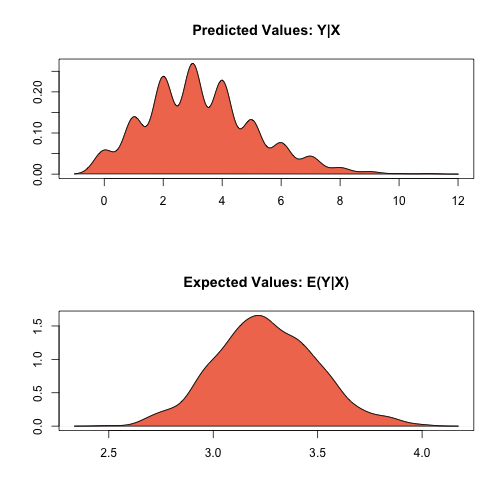
\includegraphics{Zelig-poisson-1.png}
\caption{Zelig-poisson}\end{figure}


\subsection{Model}
\label{vignette:id42}
Let \(Y_i\) be the number of independent events that occur during a
fixed time period. This variable can take any non-negative integer.
\begin{itemize}
\item {} 
The Poisson distribution has \emph{stochastic component}
\begin{gather}
\begin{split}Y_i \; \sim \; \textrm{Poisson}(\lambda_i),\end{split}\notag
\end{gather}
where \(\lambda_i\) is the mean and variance parameter.

\item {} 
The \emph{systematic component} is
\begin{gather}
\begin{split}\lambda_i \; = \; \exp(x_i \beta),\end{split}\notag
\end{gather}
where \(x_i\) is the vector of explanatory variables, and
\(\beta\) is the vector of coefficients.

\end{itemize}


\subsection{Quantities of Interest}
\label{vignette:id43}\begin{itemize}
\item {} 
The expected value (qi\$ev) is the mean of simulations from the
stochastic component,
\begin{gather}
\begin{split}E(Y) = \lambda_i =  \exp(x_i
  \beta),\end{split}\notag
\end{gather}
given draws of \(\beta\) from its sampling distribution.

\item {} 
The predicted value (qi\$pr) is a random draw from the poisson
distribution defined by mean \(\lambda_i\).

\item {} 
The first difference in the expected values (qi\$fd) is given by:
\begin{gather}
\begin{split}\textrm{FD} \; = \; E(Y | x_1) - E(Y \mid x)\end{split}\notag
\end{gather}
\item {} 
In conditional prediction models, the average expected treatment
effect (att.ev) for the treatment group is
\begin{gather}
\begin{split}\frac{1}{\sum_{i=1}^n t_i}\sum_{i:t_i=1}^n \left\{ Y_i(t_i=1) -
      E[Y_i(t_i=0)] \right\},\end{split}\notag
\end{gather}
where \(t_i\) is a binary explanatory variable defining the
treatment (\(t_i=1\)) and control (\(t_i=0\)) groups.
Variation in the simulations are due to uncertainty in simulating
\(E[Y_i(t_i=0)]\), the counterfactual expected value of
\(Y_i\) for observations in the treatment group, under the
assumption that everything stays the same except that the treatment
indicator is switched to \(t_i=0\).

\item {} 
In conditional prediction models, the average predicted treatment
effect (att.pr) for the treatment group is
\begin{gather}
\begin{split}\frac{1}{\sum_{i=1}^n t_i}\sum_{i:t_i=1}^n \left\{ Y_i(t_i=1) -
      \widehat{Y_i(t_i=0)} \right\},\end{split}\notag
\end{gather}
where \(t_i\) is a binary explanatory variable defining the
treatment (\(t_i=1\)) and control (\(t_i=0\)) groups.
Variation in the simulations are due to uncertainty in simulating
\(\widehat{Y_i(t_i=0)}\), the counterfactual predicted value of
\(Y_i\) for observations in the treatment group, under the
assumption that everything stays the same except that the treatment
indicator is switched to \(t_i=0\).

\end{itemize}


\subsection{Output Values}
\label{vignette:id44}
The output of each Zelig command contains useful information which you
may view. For example, if you run
\code{z.out \textless{}- zelig(y \textasciitilde{} x, model = poisson, data)}, then you may examine
the available information in \code{z.out} by using \code{names(z.out)}, see
the coefficients by using z.out\$coefficients, and a default summary of
information through \code{summary(z.out)}.


\subsection{See also}
\label{vignette:id45}
The poisson model is part of the stats package by . Advanced users may
wish to refer to \code{help(glm)} and \code{help(family)}.


\bigskip\hrule{}\bigskip



\section{zelig-probit}
\label{vignette:zelig-probit}\label{vignette:zprobit}
Probit Regression for Dichotomous Dependent Variables

Use probit regression to model binary dependent variables specified as a
function of a set of explanatory variables.


\subsection{Syntax}
\label{vignette:id46}
With reference classes:

\begin{Verbatim}[commandchars=\\\{\}]
z5 \PYG{o}{\PYGZlt{}\PYGZhy{}} zprobit\PYG{o}{\PYGZdl{}}new\PYG{p}{(}\PYG{p}{)}
z5\PYG{o}{\PYGZdl{}}zelig\PYG{p}{(}Y \PYG{o}{\PYGZti{}} X1 \PYG{o}{+} X \PYG{o}{\PYGZti{}} X\PYG{p}{,} data \PYG{o}{=} mydata\PYG{p}{)}
z5\PYG{o}{\PYGZdl{}}setx\PYG{p}{(}\PYG{p}{)}
z5\PYG{o}{\PYGZdl{}}sim\PYG{p}{(}\PYG{p}{)}
\end{Verbatim}

With the Zelig 4 compatibility wrappers:

\begin{Verbatim}[commandchars=\\\{\}]
z.out \PYG{o}{\PYGZlt{}\PYGZhy{}} zelig\PYG{p}{(}Y \PYG{o}{\PYGZti{}} X1 \PYG{o}{+} X2\PYG{p}{,} model \PYG{o}{=} \PYG{l+s}{\PYGZdq{}}\PYG{l+s}{probit\PYGZdq{}}\PYG{p}{,} data \PYG{o}{=} mydata\PYG{p}{)}
x.out \PYG{o}{\PYGZlt{}\PYGZhy{}} setx\PYG{p}{(}z.out\PYG{p}{)}
s.out \PYG{o}{\PYGZlt{}\PYGZhy{}} sim\PYG{p}{(}z.out\PYG{p}{,} x \PYG{o}{=} x.out\PYG{p}{,} x1 \PYG{o}{=} \PYG{k+kc}{NULL}\PYG{p}{)}
\end{Verbatim}


\subsection{Example}
\label{vignette:id47}
Attach the sample turnout dataset:

\begin{Verbatim}[commandchars=\\\{\}]
data\PYG{p}{(}turnout\PYG{p}{)}
\end{Verbatim}

Estimate parameter values for the probit regression:

\begin{Verbatim}[commandchars=\\\{\}]
z.out \PYG{o}{\PYGZlt{}\PYGZhy{}} zelig\PYG{p}{(}vote \PYG{o}{\PYGZti{}} race \PYG{o}{+} educate\PYG{p}{,} model \PYG{o}{=} \PYG{l+s}{\PYGZdq{}}\PYG{l+s}{probit\PYGZdq{}}\PYG{p}{,} data \PYG{o}{=} turnout\PYG{p}{)}
\end{Verbatim}

\begin{Verbatim}[commandchars=\\\{\}]
\PYG{c}{\PYGZsh{}\PYGZsh{} How to cite this model in Zelig:}
\PYG{c}{\PYGZsh{}\PYGZsh{}   Kosuke Imai, Gary King, Olivia Lau. 2007.}
\PYG{c}{\PYGZsh{}\PYGZsh{}   probit: Probit Regression for Dichotomous Dependent Variables}
\PYG{c}{\PYGZsh{}\PYGZsh{}   in Kosuke Imai, Gary King, and Olivia Lau, \PYGZdq{}Zelig: Everyone\PYGZsq{}s Statistical Software,\PYGZdq{}}
\PYG{c}{\PYGZsh{}\PYGZsh{}   http://zeligproject.org/}
\end{Verbatim}

\begin{Verbatim}[commandchars=\\\{\}]
summary\PYG{p}{(}z.out\PYG{p}{)}
\end{Verbatim}

\begin{Verbatim}[commandchars=\\\{\}]
\PYG{c}{\PYGZsh{}\PYGZsh{} Model:}
\PYG{c}{\PYGZsh{}\PYGZsh{} \PYGZdl{}by}
\PYG{c}{\PYGZsh{}\PYGZsh{} [1] 1}
\PYG{c}{\PYGZsh{}\PYGZsh{}}
\PYG{c}{\PYGZsh{}\PYGZsh{}}
\PYG{c}{\PYGZsh{}\PYGZsh{} Call:  stats::glm(formula = vote \PYGZti{} race + educate, family = binomial(\PYGZdq{}probit\PYGZdq{}),}
\PYG{c}{\PYGZsh{}\PYGZsh{}     data = .)}
\PYG{c}{\PYGZsh{}\PYGZsh{}}
\PYG{c}{\PYGZsh{}\PYGZsh{} Coefficients:}
\PYG{c}{\PYGZsh{}\PYGZsh{} (Intercept)    racewhite      educate}
\PYG{c}{\PYGZsh{}\PYGZsh{}    \PYGZhy{}0.72595      0.29908      0.09712}
\PYG{c}{\PYGZsh{}\PYGZsh{}}
\PYG{c}{\PYGZsh{}\PYGZsh{} Degrees of Freedom: 1999 Total (i.e. Null);  1997 Residual}
\PYG{c}{\PYGZsh{}\PYGZsh{} Null Deviance:       2267}
\PYG{c}{\PYGZsh{}\PYGZsh{} Residual Deviance: 2136  AIC: 2142}
\PYG{c}{\PYGZsh{}\PYGZsh{} Next step: Use \PYGZsq{}setx\PYGZsq{} method}
\end{Verbatim}

Set values for the explanatory variables to their default values.

\begin{Verbatim}[commandchars=\\\{\}]
x.out \PYG{o}{\PYGZlt{}\PYGZhy{}} setx\PYG{p}{(}z.out\PYG{p}{)}
\end{Verbatim}

Simulate quantities of interest from the posterior distribution.

\begin{Verbatim}[commandchars=\\\{\}]
s.out \PYG{o}{\PYGZlt{}\PYGZhy{}} sim\PYG{p}{(}z.out\PYG{p}{,} x \PYG{o}{=} x.out\PYG{p}{)}
\end{Verbatim}

\begin{Verbatim}[commandchars=\\\{\}]
summary\PYG{p}{(}s.out\PYG{p}{)}
\end{Verbatim}

\begin{Verbatim}[commandchars=\\\{\}]
plot\PYG{p}{(}s.out1\PYG{p}{)}
\end{Verbatim}
\begin{figure}[htbp]
\centering
\capstart

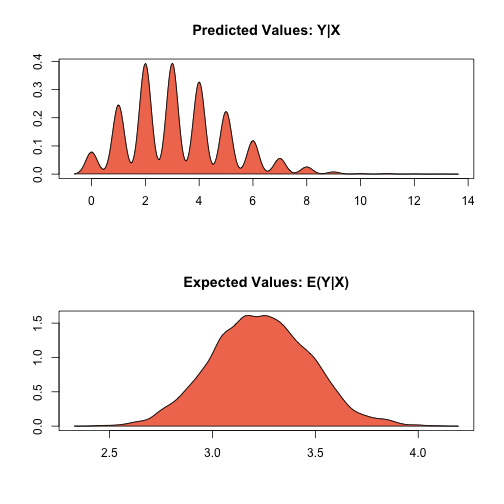
\includegraphics{Zelig-probit-1.png}
\caption{Zelig-probit}\end{figure}


\subsection{Model}
\label{vignette:id48}
Let \(Y_i\) be the observed binary dependent variable for
observation \(i\) which takes the value of either 0 or 1.
\begin{itemize}
\item {} 
The \emph{stochastic component} is given by
\begin{gather}
\begin{split}Y_i \; \sim \; \textrm{Bernoulli}(\pi_i),\end{split}\notag
\end{gather}
where \(\pi_i=\Pr(Y_i=1)\).

\item {} 
The \emph{systematic component} is
\begin{gather}
\begin{split}\pi_i \; = \; \Phi (x_i \beta)\end{split}\notag
\end{gather}
where \(\Phi(\mu)\) is the cumulative distribution function of
the Normal distribution with mean 0 and unit variance.

\end{itemize}


\subsection{Quantities of Interest}
\label{vignette:id49}\begin{itemize}
\item {} 
The expected value (qi\$ev) is a simulation of predicted probability
of success
\begin{gather}
\begin{split}E(Y) = \pi_i = \Phi(x_i
  \beta),\end{split}\notag
\end{gather}
given a draw of \(\beta\) from its sampling distribution.

\item {} 
The predicted value (qi\$pr) is a draw from a Bernoulli distribution
with mean \(\pi_i\).

\item {} 
The first difference (qi\$fd) in expected values is defined as
\begin{gather}
\begin{split}\textrm{FD} = \Pr(Y = 1 \mid x_1) - \Pr(Y = 1 \mid x).\end{split}\notag
\end{gather}
\item {} 
The risk ratio (qi\$rr) is defined as
\begin{gather}
\begin{split}\textrm{RR} = \Pr(Y = 1 \mid x_1) / \Pr(Y = 1 \mid x).\end{split}\notag
\end{gather}
\item {} 
In conditional prediction models, the average expected treatment
effect (att.ev) for the treatment group is
\begin{gather}
\begin{split}\frac{1}{\sum_{i=1}^n t_i}\sum_{i:t_i=1}^n \left\{ Y_i(t_i=1) -
      E[Y_i(t_i=0)] \right\},\end{split}\notag
\end{gather}
where \(t_i\) is a binary explanatory variable defining the
treatment (\(t_i=1\)) and control (\(t_i=0\)) groups.
Variation in the simulations are due to uncertainty in simulating
\(E[Y_i(t_i=0)]\), the counterfactual expected value of
\(Y_i\) for observations in the treatment group, under the
assumption that everything stays the same except that the treatment
indicator is switched to \(t_i=0\).

\item {} 
In conditional prediction models, the average predicted treatment
effect (att.pr) for the treatment group is
\begin{gather}
\begin{split}\frac{1}{\sum_{i=1}^n t_i}\sum_{i:t_i=1}^n \left\{ Y_i(t_i=1) -
      \widehat{Y_i(t_i=0)} \right\},\end{split}\notag
\end{gather}
where \(t_i\) is a binary explanatory variable defining the
treatment (\(t_i=1\)) and control (\(t_i=0\)) groups.
Variation in the simulations are due to uncertainty in simulating
\(\widehat{Y_i(t_i=0)}\), the counterfactual predicted value of
\(Y_i\) for observations in the treatment group, under the
assumption that everything stays the same except that the treatment
indicator is switched to \(t_i=0\).

\end{itemize}


\subsection{Output Values}
\label{vignette:id50}
The output of each Zelig command contains useful information which you
may view. For example, if you run
\code{z.out \textless{}- zelig(y \textasciitilde{} x, model = probit, data)}, then you may examine
the available information in \code{z.out} by using \code{names(z.out)}, see
the coefficients by using z.out\$coefficients, and a default summary of
information through \code{summary(z.out)}.


\subsection{See also}
\label{vignette:id51}
The probit model is part of the stats package by . Advanced users may
wish to refer to \code{help(glm)} and \code{help(family)}.


\bigskip\hrule{}\bigskip



\section{zelig-relogit}
\label{vignette:zrelogit}\label{vignette:zelig-relogit}
Rare Events Logistic Regression for Dichotomous Dependent Variables

The relogit procedure estimates the same model as standard logistic
regression (appropriate when you have a dichotomous dependent variable
and a set of explanatory variables; see ), but the estimates are
corrected for the bias that occurs when the sample is small or the
observed events are rare (i.e., if the dependent variable has many more
1s than 0s or the reverse). The relogit procedure also optionally uses
prior correction for case-control sampling designs.


\subsection{Syntax}
\label{vignette:id52}
With reference classes:

\begin{Verbatim}[commandchars=\\\{\}]
z5 \PYG{o}{\PYGZlt{}\PYGZhy{}} zrelogit\PYG{o}{\PYGZdl{}}new\PYG{p}{(}\PYG{p}{)}
z5\PYG{o}{\PYGZdl{}}zelig\PYG{p}{(}Y \PYG{o}{\PYGZti{}} X1 \PYG{o}{+} X2\PYG{p}{,} tau \PYG{o}{=} \PYG{k+kc}{NULL}\PYG{p}{,}
                       case.control \PYG{o}{=} c\PYG{p}{(}\PYG{l+s}{\PYGZdq{}}\PYG{l+s}{prior\PYGZdq{}}\PYG{p}{,} \PYG{l+s}{\PYGZdq{}}\PYG{l+s}{weighting\PYGZdq{}}\PYG{p}{)}\PYG{p}{,}
                       bias.correct \PYG{o}{=} \PYG{k+kc}{TRUE}\PYG{p}{,} robust \PYG{o}{=} \PYG{k+kc}{FALSE}\PYG{p}{,}
                       data \PYG{o}{=} mydata\PYG{p}{,} \PYG{k+kc}{...}\PYG{p}{)}
z5\PYG{o}{\PYGZdl{}}setx\PYG{p}{(}\PYG{p}{)}
z5\PYG{o}{\PYGZdl{}}sim\PYG{p}{(}\PYG{p}{)}
\end{Verbatim}

With the Zelig 4 compatibility wrappers:

\begin{Verbatim}[commandchars=\\\{\}]
z.out \PYG{o}{\PYGZlt{}\PYGZhy{}} zelig\PYG{p}{(}Y \PYG{o}{\PYGZti{}} X1 \PYG{o}{+} X2\PYG{p}{,} model \PYG{o}{=} \PYG{l+s}{\PYGZdq{}}\PYG{l+s}{relogit\PYGZdq{}}\PYG{p}{,} tau \PYG{o}{=} \PYG{k+kc}{NULL}\PYG{p}{,}
                       case.control \PYG{o}{=} c\PYG{p}{(}\PYG{l+s}{\PYGZdq{}}\PYG{l+s}{prior\PYGZdq{}}\PYG{p}{,} \PYG{l+s}{\PYGZdq{}}\PYG{l+s}{weighting\PYGZdq{}}\PYG{p}{)}\PYG{p}{,}
                       bias.correct \PYG{o}{=} \PYG{k+kc}{TRUE}\PYG{p}{,} robust \PYG{o}{=} \PYG{k+kc}{FALSE}\PYG{p}{,}
                       data \PYG{o}{=} mydata\PYG{p}{,} \PYG{k+kc}{...}\PYG{p}{)}
x.out \PYG{o}{\PYGZlt{}\PYGZhy{}} setx\PYG{p}{(}z.out\PYG{p}{)}
s.out \PYG{o}{\PYGZlt{}\PYGZhy{}} sim\PYG{p}{(}z.out\PYG{p}{,} x \PYG{o}{=} x.out\PYG{p}{)}
\end{Verbatim}


\subsection{Arguments}
\label{vignette:arguments}
The relogit procedure supports four optional arguments in addition to
the standard arguments for zelig(). You may additionally use:
\begin{itemize}
\item {} 
tau: a vector containing either one or two values for \(\tau\),
the true population fraction of ones. Use, for example, tau = c(0.05,
0.1) to specify that the lower bound on tau is 0.05 and the upper
bound is 0.1. If left unspecified, only finite-sample bias correction
is performed, not case-control correction.

\item {} 
case.control: if tau is specified, choose a method to correct for
case-control sampling design: “prior” (default) or “weighting”.

\item {} 
bias.correct: a logical value of TRUE (default) or FALSE indicating
whether the intercept should be corrected for finite sample (rare
events) bias.

\end{itemize}

Note that if tau = NULL, bias.correct = FALSE, the
relogit procedure performs a standard logistic regression without any
correction.


\subsection{Example 1: One Tau with Prior Correction and Bias Correction}
\label{vignette:example-1-one-tau-with-prior-correction-and-bias-correction}
Due to memory and space considerations, the data used here are a sample
drawn from the full data set used in King and Zeng, 2001, The proportion
of militarized interstate conflicts to the absence of disputes is
\(\tau = 1,042 / 303,772
\approx 0.00343\). To estimate the model,

\begin{Verbatim}[commandchars=\\\{\}]
data\PYG{p}{(}mid\PYG{p}{)}
\end{Verbatim}

\begin{Verbatim}[commandchars=\\\{\}]
z.out1 \PYG{o}{\PYGZlt{}\PYGZhy{}} zelig\PYG{p}{(}conflict \PYG{o}{\PYGZti{}} major \PYG{o}{+} contig \PYG{o}{+} power \PYG{o}{+} maxdem \PYG{o}{+} mindem \PYG{o}{+} years\PYG{p}{,} data \PYG{o}{=} mid\PYG{p}{,} model \PYG{o}{=} \PYG{l+s}{\PYGZdq{}}\PYG{l+s}{relogit\PYGZdq{}}\PYG{p}{,} tau \PYG{o}{=} \PYG{l+m}{1042}\PYG{o}{/}\PYG{l+m}{303772}\PYG{p}{)}
\end{Verbatim}

\begin{Verbatim}[commandchars=\\\{\}]
\PYG{c}{\PYGZsh{}\PYGZsh{} How to cite this model in Zelig:}
\PYG{c}{\PYGZsh{}\PYGZsh{}   Kosuke Imai, Gary King, and Olivia Lau. 2014.}
\PYG{c}{\PYGZsh{}\PYGZsh{}   relogit: Rare Events Logistic Regression for Dichotomous Dependent Variables}
\PYG{c}{\PYGZsh{}\PYGZsh{}   in Kosuke Imai, Gary King, and Olivia Lau, \PYGZdq{}Zelig: Everyone\PYGZsq{}s Statistical Software,\PYGZdq{}}
\PYG{c}{\PYGZsh{}\PYGZsh{}   http://zeligproject.org/}
\end{Verbatim}

Summarize the model output:

\begin{Verbatim}[commandchars=\\\{\}]
summary\PYG{p}{(}z.out1\PYG{p}{)}
\end{Verbatim}

\begin{Verbatim}[commandchars=\\\{\}]
\PYG{c}{\PYGZsh{}\PYGZsh{} Model:}
\PYG{c}{\PYGZsh{}\PYGZsh{} \PYGZdl{}by}
\PYG{c}{\PYGZsh{}\PYGZsh{} [1] 1}
\PYG{c}{\PYGZsh{}\PYGZsh{}}
\PYG{c}{\PYGZsh{}\PYGZsh{}}
\PYG{c}{\PYGZsh{}\PYGZsh{} Call:  relogit(formula = cbind(conflict, 1 \PYGZhy{} conflict) \PYGZti{} major + contig +}
\PYG{c}{\PYGZsh{}\PYGZsh{}     power + maxdem + mindem + years, data = ., tau = 0.00343020423212146,}
\PYG{c}{\PYGZsh{}\PYGZsh{}     bias.correct = TRUE, case.control = \PYGZdq{}prior\PYGZdq{})}
\PYG{c}{\PYGZsh{}\PYGZsh{}}
\PYG{c}{\PYGZsh{}\PYGZsh{} Coefficients:}
\PYG{c}{\PYGZsh{}\PYGZsh{} (Intercept)        major       contig        power       maxdem}
\PYG{c}{\PYGZsh{}\PYGZsh{}    \PYGZhy{}7.50836      2.43196      4.10797      1.05358      0.04804}
\PYG{c}{\PYGZsh{}\PYGZsh{}      mindem        years}
\PYG{c}{\PYGZsh{}\PYGZsh{}    \PYGZhy{}0.06413     \PYGZhy{}0.06293}
\PYG{c}{\PYGZsh{}\PYGZsh{}}
\PYG{c}{\PYGZsh{}\PYGZsh{} Degrees of Freedom: 3125 Total (i.e. Null);  3119 Residual}
\PYG{c}{\PYGZsh{}\PYGZsh{} Null Deviance:       3979}
\PYG{c}{\PYGZsh{}\PYGZsh{} Residual Deviance: 1869  AIC: 1883}
\PYG{c}{\PYGZsh{}\PYGZsh{} Next step: Use \PYGZsq{}setx\PYGZsq{} method}
\end{Verbatim}

Set the explanatory variables to their means:

\begin{Verbatim}[commandchars=\\\{\}]
x.out1 \PYG{o}{\PYGZlt{}\PYGZhy{}} setx\PYG{p}{(}z.out1\PYG{p}{)}
\end{Verbatim}

Simulate quantities of interest:

\begin{Verbatim}[commandchars=\\\{\}]
s.out1 \PYG{o}{\PYGZlt{}\PYGZhy{}} sim\PYG{p}{(}z.out1\PYG{p}{,} x \PYG{o}{=} x.out1\PYG{p}{)}
summary\PYG{p}{(}s.out1\PYG{p}{)}
\end{Verbatim}

\begin{Verbatim}[commandchars=\\\{\}]
\PYG{c}{\PYGZsh{}\PYGZsh{}}
\PYG{c}{\PYGZsh{}\PYGZsh{}  sim x :}
\PYG{c}{\PYGZsh{}\PYGZsh{}  \PYGZhy{}\PYGZhy{}\PYGZhy{}\PYGZhy{}\PYGZhy{}}
\PYG{c}{\PYGZsh{}\PYGZsh{} ev}
\PYG{c}{\PYGZsh{}\PYGZsh{}             mean          sd         50\PYGZpc{}        2.5\PYGZpc{}       97.5\PYGZpc{}}
\PYG{c}{\PYGZsh{}\PYGZsh{} [1,] 0.002402049 0.000157269 0.002399256 0.002087972 0.002716099}
\PYG{c}{\PYGZsh{}\PYGZsh{} pv}
\PYG{c}{\PYGZsh{}\PYGZsh{}          0     1}
\PYG{c}{\PYGZsh{}\PYGZsh{} [1,] 0.997 0.003}
\end{Verbatim}

\begin{Verbatim}[commandchars=\\\{\}]
plot\PYG{p}{(}s.out1\PYG{p}{)}
\end{Verbatim}
\begin{figure}[htbp]
\centering
\capstart


\includegraphics{Zelig-relogit-1.png}
\caption{Zelig-relogit}\end{figure}


\subsection{Example 2: One Tau with Weighting, Robust Standard Errors, and Bias Correction}
\label{vignette:example-2-one-tau-with-weighting-robust-standard-errors-and-bias-correction}
Suppose that we wish to perform case control correction using weighting
(rather than the default prior correction). To estimate the model:

\begin{Verbatim}[commandchars=\\\{\}]
z.out2 \PYG{o}{\PYGZlt{}\PYGZhy{}} zelig\PYG{p}{(}conflict \PYG{o}{\PYGZti{}} major \PYG{o}{+} contig \PYG{o}{+} power \PYG{o}{+} maxdem \PYG{o}{+} mindem \PYG{o}{+} years\PYG{p}{,} data \PYG{o}{=} mid\PYG{p}{,} model \PYG{o}{=} \PYG{l+s}{\PYGZdq{}}\PYG{l+s}{relogit\PYGZdq{}}\PYG{p}{,} tau \PYG{o}{=} \PYG{l+m}{1042}\PYG{o}{/}\PYG{l+m}{303772}\PYG{p}{,} case.control \PYG{o}{=} \PYG{l+s}{\PYGZdq{}}\PYG{l+s}{weighting\PYGZdq{}}\PYG{p}{,} robust \PYG{o}{=} \PYG{k+kc}{TRUE}\PYG{p}{)}
\end{Verbatim}

\begin{Verbatim}[commandchars=\\\{\}]
\PYG{c}{\PYGZsh{}\PYGZsh{} Error in glm.control(robust = TRUE): unused argument (robust = TRUE)}
\end{Verbatim}

Summarize the model output:

\begin{Verbatim}[commandchars=\\\{\}]
summary\PYG{p}{(}z.out2\PYG{p}{)}
\end{Verbatim}

\begin{Verbatim}[commandchars=\\\{\}]
\PYG{c}{\PYGZsh{}\PYGZsh{} Model:}
\PYG{c}{\PYGZsh{}\PYGZsh{} \PYGZdl{}by}
\PYG{c}{\PYGZsh{}\PYGZsh{} [1] 1}
\PYG{c}{\PYGZsh{}\PYGZsh{}}
\PYG{c}{\PYGZsh{}\PYGZsh{}}
\PYG{c}{\PYGZsh{}\PYGZsh{} Call:  stats::glm(formula = vote \PYGZti{} race + educate, family = binomial(\PYGZdq{}logit\PYGZdq{}),}
\PYG{c}{\PYGZsh{}\PYGZsh{}     data = .)}
\PYG{c}{\PYGZsh{}\PYGZsh{}}
\PYG{c}{\PYGZsh{}\PYGZsh{} Coefficients:}
\PYG{c}{\PYGZsh{}\PYGZsh{} (Intercept)    racewhite      educate}
\PYG{c}{\PYGZsh{}\PYGZsh{}     \PYGZhy{}1.2189       0.5022       0.1610}
\PYG{c}{\PYGZsh{}\PYGZsh{}}
\PYG{c}{\PYGZsh{}\PYGZsh{} Degrees of Freedom: 1999 Total (i.e. Null);  1997 Residual}
\PYG{c}{\PYGZsh{}\PYGZsh{} Null Deviance:       2267}
\PYG{c}{\PYGZsh{}\PYGZsh{} Residual Deviance: 2138  AIC: 2144}
\PYG{c}{\PYGZsh{}\PYGZsh{} Next step: Use \PYGZsq{}setx\PYGZsq{} method}
\end{Verbatim}

Set the explanatory variables to their means:

\begin{Verbatim}[commandchars=\\\{\}]
x.out2 \PYG{o}{\PYGZlt{}\PYGZhy{}} setx\PYG{p}{(}z.out2\PYG{p}{)}
\end{Verbatim}

Simulate quantities of interest:

\begin{Verbatim}[commandchars=\\\{\}]
s.out2 \PYG{o}{\PYGZlt{}\PYGZhy{}} sim\PYG{p}{(}z.out2\PYG{p}{,} x \PYG{o}{=} x.out2\PYG{p}{)}
summary\PYG{p}{(}s.out2\PYG{p}{)}
\end{Verbatim}

\begin{Verbatim}[commandchars=\\\{\}]
\PYG{c}{\PYGZsh{}\PYGZsh{}}
\PYG{c}{\PYGZsh{}\PYGZsh{}  sim x :}
\PYG{c}{\PYGZsh{}\PYGZsh{}  \PYGZhy{}\PYGZhy{}\PYGZhy{}\PYGZhy{}\PYGZhy{}}
\PYG{c}{\PYGZsh{}\PYGZsh{} ev}
\PYG{c}{\PYGZsh{}\PYGZsh{}           mean         sd      50\PYGZpc{}      2.5\PYGZpc{}     97.5\PYGZpc{}}
\PYG{c}{\PYGZsh{}\PYGZsh{} [1,] 0.7724619 0.01000481 0.772542 0.7532891 0.7918851}
\PYG{c}{\PYGZsh{}\PYGZsh{} pv}
\PYG{c}{\PYGZsh{}\PYGZsh{}          0     1}
\PYG{c}{\PYGZsh{}\PYGZsh{} [1,] 0.202 0.798}
\end{Verbatim}


\subsection{Example 3: Two Taus with Bias Correction and Prior Correction}
\label{vignette:example-3-two-taus-with-bias-correction-and-prior-correction}
Suppose that we did not know that \(\tau \approx 0.00343\), but only
that it was somewhere between \((0.002, 0.005)\). To estimate a
model with a range of feasible estimates for \(\tau\) (using the
default prior correction method for case control correction):

\begin{Verbatim}[commandchars=\\\{\}]
z.out2 \PYG{o}{\PYGZlt{}\PYGZhy{}} zelig\PYG{p}{(}conflict \PYG{o}{\PYGZti{}} major \PYG{o}{+} contig \PYG{o}{+} power \PYG{o}{+} maxdem \PYG{o}{+} mindem \PYG{o}{+} years\PYG{p}{,} data \PYG{o}{=} mid\PYG{p}{,} model \PYG{o}{=} \PYG{l+s}{\PYGZdq{}}\PYG{l+s}{relogit\PYGZdq{}}\PYG{p}{,} tau \PYG{o}{=} c\PYG{p}{(}\PYG{l+m}{0.002}\PYG{p}{,} \PYG{l+m}{0.005}\PYG{p}{)}\PYG{p}{)}
\end{Verbatim}

\begin{Verbatim}[commandchars=\\\{\}]
\PYG{c}{\PYGZsh{}\PYGZsh{} How to cite this model in Zelig:}
\PYG{c}{\PYGZsh{}\PYGZsh{}   Kosuke Imai, Gary King, and Olivia Lau. 2014.}
\PYG{c}{\PYGZsh{}\PYGZsh{}   relogit: Rare Events Logistic Regression for Dichotomous Dependent Variables}
\PYG{c}{\PYGZsh{}\PYGZsh{}   in Kosuke Imai, Gary King, and Olivia Lau, \PYGZdq{}Zelig: Everyone\PYGZsq{}s Statistical Software,\PYGZdq{}}
\PYG{c}{\PYGZsh{}\PYGZsh{}   http://zeligproject.org/}
\end{Verbatim}

Summarize the model output:

\begin{Verbatim}[commandchars=\\\{\}]
z.out2
\end{Verbatim}

\begin{Verbatim}[commandchars=\\\{\}]
\PYG{c}{\PYGZsh{}\PYGZsh{} Model:}
\PYG{c}{\PYGZsh{}\PYGZsh{} \PYGZdl{}by}
\PYG{c}{\PYGZsh{}\PYGZsh{} [1] 1}
\PYG{c}{\PYGZsh{}\PYGZsh{}}
\PYG{c}{\PYGZsh{}\PYGZsh{} \PYGZdl{}lower.estimate}
\PYG{c}{\PYGZsh{}\PYGZsh{}}
\PYG{c}{\PYGZsh{}\PYGZsh{} Call:  (function (formula, data = sys.parent(), tau = NULL, bias.correct = TRUE,}
\PYG{c}{\PYGZsh{}\PYGZsh{}     case.control = \PYGZdq{}prior\PYGZdq{}, ...)}
\PYG{c}{\PYGZsh{}\PYGZsh{} \PYGZob{}}
\PYG{c}{\PYGZsh{}\PYGZsh{}     mf \PYGZlt{}\PYGZhy{} match.call()}
\PYG{c}{\PYGZsh{}\PYGZsh{}     mf\PYGZdl{}tau \PYGZlt{}\PYGZhy{} mf\PYGZdl{}bias.correct \PYGZlt{}\PYGZhy{} mf\PYGZdl{}case.control \PYGZlt{}\PYGZhy{} NULL}
\PYG{c}{\PYGZsh{}\PYGZsh{}     if (!is.null(tau)) \PYGZob{}}
\PYG{c}{\PYGZsh{}\PYGZsh{}         tau \PYGZlt{}\PYGZhy{} unique(tau)}
\PYG{c}{\PYGZsh{}\PYGZsh{}         if (length(case.control) \PYGZgt{} 1)}
\PYG{c}{\PYGZsh{}\PYGZsh{}             stop(\PYGZdq{}You can only choose one option for case control correction.\PYGZdq{})}
\PYG{c}{\PYGZsh{}\PYGZsh{}         ck1 \PYGZlt{}\PYGZhy{} grep(\PYGZdq{}p\PYGZdq{}, case.control)}
\PYG{c}{\PYGZsh{}\PYGZsh{}         ck2 \PYGZlt{}\PYGZhy{} grep(\PYGZdq{}w\PYGZdq{}, case.control)}
\PYG{c}{\PYGZsh{}\PYGZsh{}         if (length(ck1) == 0 \PYGZam{} length(ck2) == 0)}
\PYG{c}{\PYGZsh{}\PYGZsh{}             stop(\PYGZdq{}choose either case.control = \PYGZbs{}\PYGZdq{}prior\PYGZbs{}\PYGZdq{} \PYGZdq{}, \PYGZdq{}or case.control = \PYGZbs{}\PYGZdq{}weighting\PYGZbs{}\PYGZdq{}\PYGZdq{})}
\PYG{c}{\PYGZsh{}\PYGZsh{}         if (length(ck2) == 0)}
\PYG{c}{\PYGZsh{}\PYGZsh{}             weighting \PYGZlt{}\PYGZhy{} FALSE}
\PYG{c}{\PYGZsh{}\PYGZsh{}         else weighting \PYGZlt{}\PYGZhy{} TRUE}
\PYG{c}{\PYGZsh{}\PYGZsh{}     \PYGZcb{}}
\PYG{c}{\PYGZsh{}\PYGZsh{}     else weighting \PYGZlt{}\PYGZhy{} FALSE}
\PYG{c}{\PYGZsh{}\PYGZsh{}     if (length(tau) \PYGZgt{} 2)}
\PYG{c}{\PYGZsh{}\PYGZsh{}         stop(\PYGZdq{}tau must be a vector of length less than or equal to 2\PYGZdq{})}
\PYG{c}{\PYGZsh{}\PYGZsh{}     else if (length(tau) == 2) \PYGZob{}}
\PYG{c}{\PYGZsh{}\PYGZsh{}         mf[[1]] \PYGZlt{}\PYGZhy{} relogit}
\PYG{c}{\PYGZsh{}\PYGZsh{}         res \PYGZlt{}\PYGZhy{} list()}
\PYG{c}{\PYGZsh{}\PYGZsh{}         mf\PYGZdl{}tau \PYGZlt{}\PYGZhy{} min(tau)}
\PYG{c}{\PYGZsh{}\PYGZsh{}         res\PYGZdl{}lower.estimate \PYGZlt{}\PYGZhy{} eval(as.call(mf), parent.frame())}
\PYG{c}{\PYGZsh{}\PYGZsh{}         mf\PYGZdl{}tau \PYGZlt{}\PYGZhy{} max(tau)}
\PYG{c}{\PYGZsh{}\PYGZsh{}         res\PYGZdl{}upper.estimate \PYGZlt{}\PYGZhy{} eval(as.call(mf), parent.frame())}
\PYG{c}{\PYGZsh{}\PYGZsh{}         res\PYGZdl{}formula \PYGZlt{}\PYGZhy{} formula}
\PYG{c}{\PYGZsh{}\PYGZsh{}         class(res) \PYGZlt{}\PYGZhy{} c(\PYGZdq{}Relogit2\PYGZdq{}, \PYGZdq{}Relogit\PYGZdq{})}
\PYG{c}{\PYGZsh{}\PYGZsh{}         return(res)}
\PYG{c}{\PYGZsh{}\PYGZsh{}     \PYGZcb{}}
\PYG{c}{\PYGZsh{}\PYGZsh{}     else \PYGZob{}}
\PYG{c}{\PYGZsh{}\PYGZsh{}         mf[[1]] \PYGZlt{}\PYGZhy{} glm}
\PYG{c}{\PYGZsh{}\PYGZsh{}         mf\PYGZdl{}family \PYGZlt{}\PYGZhy{} binomial(link = \PYGZdq{}logit\PYGZdq{})}
\PYG{c}{\PYGZsh{}\PYGZsh{}         y2 \PYGZlt{}\PYGZhy{} model.response(model.frame(mf\PYGZdl{}formula, data))}
\PYG{c}{\PYGZsh{}\PYGZsh{}         if (is.matrix(y2))}
\PYG{c}{\PYGZsh{}\PYGZsh{}             y \PYGZlt{}\PYGZhy{} y2[, 1]}
\PYG{c}{\PYGZsh{}\PYGZsh{}         else y \PYGZlt{}\PYGZhy{} y2}
\PYG{c}{\PYGZsh{}\PYGZsh{}         ybar \PYGZlt{}\PYGZhy{} mean(y)}
\PYG{c}{\PYGZsh{}\PYGZsh{}         if (weighting) \PYGZob{}}
\PYG{c}{\PYGZsh{}\PYGZsh{}             w1 \PYGZlt{}\PYGZhy{} tau/ybar}
\PYG{c}{\PYGZsh{}\PYGZsh{}             w0 \PYGZlt{}\PYGZhy{} (1 \PYGZhy{} tau)/(1 \PYGZhy{} ybar)}
\PYG{c}{\PYGZsh{}\PYGZsh{}             wi \PYGZlt{}\PYGZhy{} w1 * y + w0 * (1 \PYGZhy{} y)}
\PYG{c}{\PYGZsh{}\PYGZsh{}             mf\PYGZdl{}weights \PYGZlt{}\PYGZhy{} wi}
\PYG{c}{\PYGZsh{}\PYGZsh{}         \PYGZcb{}}
\PYG{c}{\PYGZsh{}\PYGZsh{}         res \PYGZlt{}\PYGZhy{} eval(as.call(mf), parent.frame())}
\PYG{c}{\PYGZsh{}\PYGZsh{}         res\PYGZdl{}call \PYGZlt{}\PYGZhy{} match.call(expand.dots = TRUE)}
\PYG{c}{\PYGZsh{}\PYGZsh{}         res\PYGZdl{}tau \PYGZlt{}\PYGZhy{} tau}
\PYG{c}{\PYGZsh{}\PYGZsh{}         X \PYGZlt{}\PYGZhy{} model.matrix(res)}
\PYG{c}{\PYGZsh{}\PYGZsh{}         if (bias.correct) \PYGZob{}}
\PYG{c}{\PYGZsh{}\PYGZsh{}             pihat \PYGZlt{}\PYGZhy{} fitted(res)}
\PYG{c}{\PYGZsh{}\PYGZsh{}             if (is.null(tau))}
\PYG{c}{\PYGZsh{}\PYGZsh{}                 wi \PYGZlt{}\PYGZhy{} rep(1, length(y))}
\PYG{c}{\PYGZsh{}\PYGZsh{}             else if (weighting)}
\PYG{c}{\PYGZsh{}\PYGZsh{}                 res\PYGZdl{}weighting \PYGZlt{}\PYGZhy{} TRUE}
\PYG{c}{\PYGZsh{}\PYGZsh{}             else \PYGZob{}}
\PYG{c}{\PYGZsh{}\PYGZsh{}                 w1 \PYGZlt{}\PYGZhy{} tau/ybar}
\PYG{c}{\PYGZsh{}\PYGZsh{}                 w0 \PYGZlt{}\PYGZhy{} (1 \PYGZhy{} tau)/(1 \PYGZhy{} ybar)}
\PYG{c}{\PYGZsh{}\PYGZsh{}                 wi \PYGZlt{}\PYGZhy{} w1 * y + w0 * (1 \PYGZhy{} y)}
\PYG{c}{\PYGZsh{}\PYGZsh{}                 res\PYGZdl{}weighting \PYGZlt{}\PYGZhy{} FALSE}
\PYG{c}{\PYGZsh{}\PYGZsh{}             \PYGZcb{}}
\PYG{c}{\PYGZsh{}\PYGZsh{}             W \PYGZlt{}\PYGZhy{} pihat * (1 \PYGZhy{} pihat) * wi}
\PYG{c}{\PYGZsh{}\PYGZsh{}             Qdiag \PYGZlt{}\PYGZhy{} lm.influence(lm(y \PYGZti{} X \PYGZhy{} 1, weights = W))\PYGZdl{}hat/W}
\PYG{c}{\PYGZsh{}\PYGZsh{}             if (is.null(tau))}
\PYG{c}{\PYGZsh{}\PYGZsh{}                 xi \PYGZlt{}\PYGZhy{} 0.5 * Qdiag * (2 * pihat \PYGZhy{} 1)}
\PYG{c}{\PYGZsh{}\PYGZsh{}             else xi \PYGZlt{}\PYGZhy{} 0.5 * Qdiag * ((1 + w0) * pihat \PYGZhy{} w0)}
\PYG{c}{\PYGZsh{}\PYGZsh{}             res\PYGZdl{}coefficients \PYGZlt{}\PYGZhy{} res\PYGZdl{}coefficients \PYGZhy{} lm(xi \PYGZti{} X \PYGZhy{}}
\PYG{c}{\PYGZsh{}\PYGZsh{}                 1, weights = W)\PYGZdl{}coefficients}
\PYG{c}{\PYGZsh{}\PYGZsh{}             res\PYGZdl{}bias.correct \PYGZlt{}\PYGZhy{} TRUE}
\PYG{c}{\PYGZsh{}\PYGZsh{}         \PYGZcb{}}
\PYG{c}{\PYGZsh{}\PYGZsh{}         else res\PYGZdl{}bias.correct \PYGZlt{}\PYGZhy{} FALSE}
\PYG{c}{\PYGZsh{}\PYGZsh{}         if (!is.null(tau) \PYGZam{} !weighting) \PYGZob{}}
\PYG{c}{\PYGZsh{}\PYGZsh{}             if (tau \PYGZlt{}= 0 \textbar{}\textbar{} tau \PYGZgt{}= 1)}
\PYG{c}{\PYGZsh{}\PYGZsh{}                 stop(\PYGZdq{}\PYGZbs{}ntau needs to be between 0 and 1.\PYGZbs{}n\PYGZdq{})}
\PYG{c}{\PYGZsh{}\PYGZsh{}             res\PYGZdl{}coefficients[\PYGZdq{}(Intercept)\PYGZdq{}] \PYGZlt{}\PYGZhy{} res\PYGZdl{}coefficients[\PYGZdq{}(Intercept)\PYGZdq{}] \PYGZhy{}}
\PYG{c}{\PYGZsh{}\PYGZsh{}                 log(((1 \PYGZhy{} tau)/tau) * (ybar/(1 \PYGZhy{} ybar)))}
\PYG{c}{\PYGZsh{}\PYGZsh{}             res\PYGZdl{}prior.correct \PYGZlt{}\PYGZhy{} TRUE}
\PYG{c}{\PYGZsh{}\PYGZsh{}             res\PYGZdl{}weighting \PYGZlt{}\PYGZhy{} FALSE}
\PYG{c}{\PYGZsh{}\PYGZsh{}         \PYGZcb{}}
\PYG{c}{\PYGZsh{}\PYGZsh{}         else res\PYGZdl{}prior.correct \PYGZlt{}\PYGZhy{} FALSE}
\PYG{c}{\PYGZsh{}\PYGZsh{}         if (is.null(res\PYGZdl{}weighting))}
\PYG{c}{\PYGZsh{}\PYGZsh{}             res\PYGZdl{}weighting \PYGZlt{}\PYGZhy{} FALSE}
\PYG{c}{\PYGZsh{}\PYGZsh{}         res\PYGZdl{}linear.predictors \PYGZlt{}\PYGZhy{} t(res\PYGZdl{}coefficients) \PYGZpc{}*\PYGZpc{} t(X)}
\PYG{c}{\PYGZsh{}\PYGZsh{}         res\PYGZdl{}fitted.values \PYGZlt{}\PYGZhy{} 1/(1 + exp(\PYGZhy{}res\PYGZdl{}linear.predictors))}
\PYG{c}{\PYGZsh{}\PYGZsh{}         res\PYGZdl{}zelig \PYGZlt{}\PYGZhy{} \PYGZdq{}Relogit\PYGZdq{}}
\PYG{c}{\PYGZsh{}\PYGZsh{}         class(res) \PYGZlt{}\PYGZhy{} c(\PYGZdq{}Relogit\PYGZdq{}, \PYGZdq{}glm\PYGZdq{})}
\PYG{c}{\PYGZsh{}\PYGZsh{}         return(res)}
\PYG{c}{\PYGZsh{}\PYGZsh{}     \PYGZcb{}}
\PYG{c}{\PYGZsh{}\PYGZsh{} \PYGZcb{})(formula = cbind(conflict, 1 \PYGZhy{} conflict) \PYGZti{} major + contig +}
\PYG{c}{\PYGZsh{}\PYGZsh{}     power + maxdem + mindem + years, data = ., tau = 0.002)}
\PYG{c}{\PYGZsh{}\PYGZsh{}}
\PYG{c}{\PYGZsh{}\PYGZsh{} Coefficients:}
\PYG{c}{\PYGZsh{}\PYGZsh{} (Intercept)        major       contig        power       maxdem}
\PYG{c}{\PYGZsh{}\PYGZsh{}    \PYGZhy{}8.04923      2.43196      4.10791      1.05357      0.04804}
\PYG{c}{\PYGZsh{}\PYGZsh{}      mindem        years}
\PYG{c}{\PYGZsh{}\PYGZsh{}    \PYGZhy{}0.06412     \PYGZhy{}0.06293}
\PYG{c}{\PYGZsh{}\PYGZsh{}}
\PYG{c}{\PYGZsh{}\PYGZsh{} Degrees of Freedom: 3125 Total (i.e. Null);  3119 Residual}
\PYG{c}{\PYGZsh{}\PYGZsh{} Null Deviance:       3979}
\PYG{c}{\PYGZsh{}\PYGZsh{} Residual Deviance: 1869  AIC: 1883}
\PYG{c}{\PYGZsh{}\PYGZsh{}}
\PYG{c}{\PYGZsh{}\PYGZsh{} \PYGZdl{}upper.estimate}
\PYG{c}{\PYGZsh{}\PYGZsh{}}
\PYG{c}{\PYGZsh{}\PYGZsh{} Call:  (function (formula, data = sys.parent(), tau = NULL, bias.correct = TRUE,}
\PYG{c}{\PYGZsh{}\PYGZsh{}     case.control = \PYGZdq{}prior\PYGZdq{}, ...)}
\PYG{c}{\PYGZsh{}\PYGZsh{} \PYGZob{}}
\PYG{c}{\PYGZsh{}\PYGZsh{}     mf \PYGZlt{}\PYGZhy{} match.call()}
\PYG{c}{\PYGZsh{}\PYGZsh{}     mf\PYGZdl{}tau \PYGZlt{}\PYGZhy{} mf\PYGZdl{}bias.correct \PYGZlt{}\PYGZhy{} mf\PYGZdl{}case.control \PYGZlt{}\PYGZhy{} NULL}
\PYG{c}{\PYGZsh{}\PYGZsh{}     if (!is.null(tau)) \PYGZob{}}
\PYG{c}{\PYGZsh{}\PYGZsh{}         tau \PYGZlt{}\PYGZhy{} unique(tau)}
\PYG{c}{\PYGZsh{}\PYGZsh{}         if (length(case.control) \PYGZgt{} 1)}
\PYG{c}{\PYGZsh{}\PYGZsh{}             stop(\PYGZdq{}You can only choose one option for case control correction.\PYGZdq{})}
\PYG{c}{\PYGZsh{}\PYGZsh{}         ck1 \PYGZlt{}\PYGZhy{} grep(\PYGZdq{}p\PYGZdq{}, case.control)}
\PYG{c}{\PYGZsh{}\PYGZsh{}         ck2 \PYGZlt{}\PYGZhy{} grep(\PYGZdq{}w\PYGZdq{}, case.control)}
\PYG{c}{\PYGZsh{}\PYGZsh{}         if (length(ck1) == 0 \PYGZam{} length(ck2) == 0)}
\PYG{c}{\PYGZsh{}\PYGZsh{}             stop(\PYGZdq{}choose either case.control = \PYGZbs{}\PYGZdq{}prior\PYGZbs{}\PYGZdq{} \PYGZdq{}, \PYGZdq{}or case.control = \PYGZbs{}\PYGZdq{}weighting\PYGZbs{}\PYGZdq{}\PYGZdq{})}
\PYG{c}{\PYGZsh{}\PYGZsh{}         if (length(ck2) == 0)}
\PYG{c}{\PYGZsh{}\PYGZsh{}             weighting \PYGZlt{}\PYGZhy{} FALSE}
\PYG{c}{\PYGZsh{}\PYGZsh{}         else weighting \PYGZlt{}\PYGZhy{} TRUE}
\PYG{c}{\PYGZsh{}\PYGZsh{}     \PYGZcb{}}
\PYG{c}{\PYGZsh{}\PYGZsh{}     else weighting \PYGZlt{}\PYGZhy{} FALSE}
\PYG{c}{\PYGZsh{}\PYGZsh{}     if (length(tau) \PYGZgt{} 2)}
\PYG{c}{\PYGZsh{}\PYGZsh{}         stop(\PYGZdq{}tau must be a vector of length less than or equal to 2\PYGZdq{})}
\PYG{c}{\PYGZsh{}\PYGZsh{}     else if (length(tau) == 2) \PYGZob{}}
\PYG{c}{\PYGZsh{}\PYGZsh{}         mf[[1]] \PYGZlt{}\PYGZhy{} relogit}
\PYG{c}{\PYGZsh{}\PYGZsh{}         res \PYGZlt{}\PYGZhy{} list()}
\PYG{c}{\PYGZsh{}\PYGZsh{}         mf\PYGZdl{}tau \PYGZlt{}\PYGZhy{} min(tau)}
\PYG{c}{\PYGZsh{}\PYGZsh{}         res\PYGZdl{}lower.estimate \PYGZlt{}\PYGZhy{} eval(as.call(mf), parent.frame())}
\PYG{c}{\PYGZsh{}\PYGZsh{}         mf\PYGZdl{}tau \PYGZlt{}\PYGZhy{} max(tau)}
\PYG{c}{\PYGZsh{}\PYGZsh{}         res\PYGZdl{}upper.estimate \PYGZlt{}\PYGZhy{} eval(as.call(mf), parent.frame())}
\PYG{c}{\PYGZsh{}\PYGZsh{}         res\PYGZdl{}formula \PYGZlt{}\PYGZhy{} formula}
\PYG{c}{\PYGZsh{}\PYGZsh{}         class(res) \PYGZlt{}\PYGZhy{} c(\PYGZdq{}Relogit2\PYGZdq{}, \PYGZdq{}Relogit\PYGZdq{})}
\PYG{c}{\PYGZsh{}\PYGZsh{}         return(res)}
\PYG{c}{\PYGZsh{}\PYGZsh{}     \PYGZcb{}}
\PYG{c}{\PYGZsh{}\PYGZsh{}     else \PYGZob{}}
\PYG{c}{\PYGZsh{}\PYGZsh{}         mf[[1]] \PYGZlt{}\PYGZhy{} glm}
\PYG{c}{\PYGZsh{}\PYGZsh{}         mf\PYGZdl{}family \PYGZlt{}\PYGZhy{} binomial(link = \PYGZdq{}logit\PYGZdq{})}
\PYG{c}{\PYGZsh{}\PYGZsh{}         y2 \PYGZlt{}\PYGZhy{} model.response(model.frame(mf\PYGZdl{}formula, data))}
\PYG{c}{\PYGZsh{}\PYGZsh{}         if (is.matrix(y2))}
\PYG{c}{\PYGZsh{}\PYGZsh{}             y \PYGZlt{}\PYGZhy{} y2[, 1]}
\PYG{c}{\PYGZsh{}\PYGZsh{}         else y \PYGZlt{}\PYGZhy{} y2}
\PYG{c}{\PYGZsh{}\PYGZsh{}         ybar \PYGZlt{}\PYGZhy{} mean(y)}
\PYG{c}{\PYGZsh{}\PYGZsh{}         if (weighting) \PYGZob{}}
\PYG{c}{\PYGZsh{}\PYGZsh{}             w1 \PYGZlt{}\PYGZhy{} tau/ybar}
\PYG{c}{\PYGZsh{}\PYGZsh{}             w0 \PYGZlt{}\PYGZhy{} (1 \PYGZhy{} tau)/(1 \PYGZhy{} ybar)}
\PYG{c}{\PYGZsh{}\PYGZsh{}             wi \PYGZlt{}\PYGZhy{} w1 * y + w0 * (1 \PYGZhy{} y)}
\PYG{c}{\PYGZsh{}\PYGZsh{}             mf\PYGZdl{}weights \PYGZlt{}\PYGZhy{} wi}
\PYG{c}{\PYGZsh{}\PYGZsh{}         \PYGZcb{}}
\PYG{c}{\PYGZsh{}\PYGZsh{}         res \PYGZlt{}\PYGZhy{} eval(as.call(mf), parent.frame())}
\PYG{c}{\PYGZsh{}\PYGZsh{}         res\PYGZdl{}call \PYGZlt{}\PYGZhy{} match.call(expand.dots = TRUE)}
\PYG{c}{\PYGZsh{}\PYGZsh{}         res\PYGZdl{}tau \PYGZlt{}\PYGZhy{} tau}
\PYG{c}{\PYGZsh{}\PYGZsh{}         X \PYGZlt{}\PYGZhy{} model.matrix(res)}
\PYG{c}{\PYGZsh{}\PYGZsh{}         if (bias.correct) \PYGZob{}}
\PYG{c}{\PYGZsh{}\PYGZsh{}             pihat \PYGZlt{}\PYGZhy{} fitted(res)}
\PYG{c}{\PYGZsh{}\PYGZsh{}             if (is.null(tau))}
\PYG{c}{\PYGZsh{}\PYGZsh{}                 wi \PYGZlt{}\PYGZhy{} rep(1, length(y))}
\PYG{c}{\PYGZsh{}\PYGZsh{}             else if (weighting)}
\PYG{c}{\PYGZsh{}\PYGZsh{}                 res\PYGZdl{}weighting \PYGZlt{}\PYGZhy{} TRUE}
\PYG{c}{\PYGZsh{}\PYGZsh{}             else \PYGZob{}}
\PYG{c}{\PYGZsh{}\PYGZsh{}                 w1 \PYGZlt{}\PYGZhy{} tau/ybar}
\PYG{c}{\PYGZsh{}\PYGZsh{}                 w0 \PYGZlt{}\PYGZhy{} (1 \PYGZhy{} tau)/(1 \PYGZhy{} ybar)}
\PYG{c}{\PYGZsh{}\PYGZsh{}                 wi \PYGZlt{}\PYGZhy{} w1 * y + w0 * (1 \PYGZhy{} y)}
\PYG{c}{\PYGZsh{}\PYGZsh{}                 res\PYGZdl{}weighting \PYGZlt{}\PYGZhy{} FALSE}
\PYG{c}{\PYGZsh{}\PYGZsh{}             \PYGZcb{}}
\PYG{c}{\PYGZsh{}\PYGZsh{}             W \PYGZlt{}\PYGZhy{} pihat * (1 \PYGZhy{} pihat) * wi}
\PYG{c}{\PYGZsh{}\PYGZsh{}             Qdiag \PYGZlt{}\PYGZhy{} lm.influence(lm(y \PYGZti{} X \PYGZhy{} 1, weights = W))\PYGZdl{}hat/W}
\PYG{c}{\PYGZsh{}\PYGZsh{}             if (is.null(tau))}
\PYG{c}{\PYGZsh{}\PYGZsh{}                 xi \PYGZlt{}\PYGZhy{} 0.5 * Qdiag * (2 * pihat \PYGZhy{} 1)}
\PYG{c}{\PYGZsh{}\PYGZsh{}             else xi \PYGZlt{}\PYGZhy{} 0.5 * Qdiag * ((1 + w0) * pihat \PYGZhy{} w0)}
\PYG{c}{\PYGZsh{}\PYGZsh{}             res\PYGZdl{}coefficients \PYGZlt{}\PYGZhy{} res\PYGZdl{}coefficients \PYGZhy{} lm(xi \PYGZti{} X \PYGZhy{}}
\PYG{c}{\PYGZsh{}\PYGZsh{}                 1, weights = W)\PYGZdl{}coefficients}
\PYG{c}{\PYGZsh{}\PYGZsh{}             res\PYGZdl{}bias.correct \PYGZlt{}\PYGZhy{} TRUE}
\PYG{c}{\PYGZsh{}\PYGZsh{}         \PYGZcb{}}
\PYG{c}{\PYGZsh{}\PYGZsh{}         else res\PYGZdl{}bias.correct \PYGZlt{}\PYGZhy{} FALSE}
\PYG{c}{\PYGZsh{}\PYGZsh{}         if (!is.null(tau) \PYGZam{} !weighting) \PYGZob{}}
\PYG{c}{\PYGZsh{}\PYGZsh{}             if (tau \PYGZlt{}= 0 \textbar{}\textbar{} tau \PYGZgt{}= 1)}
\PYG{c}{\PYGZsh{}\PYGZsh{}                 stop(\PYGZdq{}\PYGZbs{}ntau needs to be between 0 and 1.\PYGZbs{}n\PYGZdq{})}
\PYG{c}{\PYGZsh{}\PYGZsh{}             res\PYGZdl{}coefficients[\PYGZdq{}(Intercept)\PYGZdq{}] \PYGZlt{}\PYGZhy{} res\PYGZdl{}coefficients[\PYGZdq{}(Intercept)\PYGZdq{}] \PYGZhy{}}
\PYG{c}{\PYGZsh{}\PYGZsh{}                 log(((1 \PYGZhy{} tau)/tau) * (ybar/(1 \PYGZhy{} ybar)))}
\PYG{c}{\PYGZsh{}\PYGZsh{}             res\PYGZdl{}prior.correct \PYGZlt{}\PYGZhy{} TRUE}
\PYG{c}{\PYGZsh{}\PYGZsh{}             res\PYGZdl{}weighting \PYGZlt{}\PYGZhy{} FALSE}
\PYG{c}{\PYGZsh{}\PYGZsh{}         \PYGZcb{}}
\PYG{c}{\PYGZsh{}\PYGZsh{}         else res\PYGZdl{}prior.correct \PYGZlt{}\PYGZhy{} FALSE}
\PYG{c}{\PYGZsh{}\PYGZsh{}         if (is.null(res\PYGZdl{}weighting))}
\PYG{c}{\PYGZsh{}\PYGZsh{}             res\PYGZdl{}weighting \PYGZlt{}\PYGZhy{} FALSE}
\PYG{c}{\PYGZsh{}\PYGZsh{}         res\PYGZdl{}linear.predictors \PYGZlt{}\PYGZhy{} t(res\PYGZdl{}coefficients) \PYGZpc{}*\PYGZpc{} t(X)}
\PYG{c}{\PYGZsh{}\PYGZsh{}         res\PYGZdl{}fitted.values \PYGZlt{}\PYGZhy{} 1/(1 + exp(\PYGZhy{}res\PYGZdl{}linear.predictors))}
\PYG{c}{\PYGZsh{}\PYGZsh{}         res\PYGZdl{}zelig \PYGZlt{}\PYGZhy{} \PYGZdq{}Relogit\PYGZdq{}}
\PYG{c}{\PYGZsh{}\PYGZsh{}         class(res) \PYGZlt{}\PYGZhy{} c(\PYGZdq{}Relogit\PYGZdq{}, \PYGZdq{}glm\PYGZdq{})}
\PYG{c}{\PYGZsh{}\PYGZsh{}         return(res)}
\PYG{c}{\PYGZsh{}\PYGZsh{}     \PYGZcb{}}
\PYG{c}{\PYGZsh{}\PYGZsh{} \PYGZcb{})(formula = cbind(conflict, 1 \PYGZhy{} conflict) \PYGZti{} major + contig +}
\PYG{c}{\PYGZsh{}\PYGZsh{}     power + maxdem + mindem + years, data = ., tau = 0.005)}
\PYG{c}{\PYGZsh{}\PYGZsh{}}
\PYG{c}{\PYGZsh{}\PYGZsh{} Coefficients:}
\PYG{c}{\PYGZsh{}\PYGZsh{} (Intercept)        major       contig        power       maxdem}
\PYG{c}{\PYGZsh{}\PYGZsh{}    \PYGZhy{}7.13001      2.43197      4.10805      1.05358      0.04804}
\PYG{c}{\PYGZsh{}\PYGZsh{}      mindem        years}
\PYG{c}{\PYGZsh{}\PYGZsh{}    \PYGZhy{}0.06413     \PYGZhy{}0.06294}
\PYG{c}{\PYGZsh{}\PYGZsh{}}
\PYG{c}{\PYGZsh{}\PYGZsh{} Degrees of Freedom: 3125 Total (i.e. Null);  3119 Residual}
\PYG{c}{\PYGZsh{}\PYGZsh{} Null Deviance:       3979}
\PYG{c}{\PYGZsh{}\PYGZsh{} Residual Deviance: 1869  AIC: 1883}
\PYG{c}{\PYGZsh{}\PYGZsh{}}
\PYG{c}{\PYGZsh{}\PYGZsh{} \PYGZdl{}formula}
\PYG{c}{\PYGZsh{}\PYGZsh{} cbind(conflict, 1 \PYGZhy{} conflict) \PYGZti{} major + contig + power + maxdem +}
\PYG{c}{\PYGZsh{}\PYGZsh{}     mindem + years}
\PYG{c}{\PYGZsh{}\PYGZsh{} \PYGZlt{}environment: 0x7fa7c50f1498\PYGZgt{}}
\PYG{c}{\PYGZsh{}\PYGZsh{}}
\PYG{c}{\PYGZsh{}\PYGZsh{} attr(,\PYGZdq{}class\PYGZdq{})}
\PYG{c}{\PYGZsh{}\PYGZsh{} [1] \PYGZdq{}Relogit2\PYGZdq{} \PYGZdq{}Relogit\PYGZdq{}}
\PYG{c}{\PYGZsh{}\PYGZsh{} Next step: Use \PYGZsq{}setx\PYGZsq{} method}
\end{Verbatim}

Set the explanatory variables to their means:

\begin{Verbatim}[commandchars=\\\{\}]
x.out2 \PYG{o}{\PYGZlt{}\PYGZhy{}} setx\PYG{p}{(}z.out2\PYG{p}{)}
\end{Verbatim}

Simulate quantities of interest:

\begin{Verbatim}[commandchars=\\\{\}]
s.out \PYG{o}{\PYGZlt{}\PYGZhy{}} sim\PYG{p}{(}z.out2\PYG{p}{,} x \PYG{o}{=} x.out2\PYG{p}{)}
\end{Verbatim}

\begin{Verbatim}[commandchars=\\\{\}]
\PYG{c}{\PYGZsh{}\PYGZsh{} Error in UseMethod(\PYGZdq{}vcov\PYGZdq{}): no applicable method for \PYGZsq{}vcov\PYGZsq{} applied to an object of class \PYGZdq{}c(\PYGZsq{}Relogit2\PYGZsq{}, \PYGZsq{}Relogit\PYGZsq{})\PYGZdq{}}
\end{Verbatim}

\begin{Verbatim}[commandchars=\\\{\}]
summary\PYG{p}{(}s.out2\PYG{p}{)}
\end{Verbatim}

\begin{Verbatim}[commandchars=\\\{\}]
\PYG{c}{\PYGZsh{}\PYGZsh{}}
\PYG{c}{\PYGZsh{}\PYGZsh{}  sim x :}
\PYG{c}{\PYGZsh{}\PYGZsh{}  \PYGZhy{}\PYGZhy{}\PYGZhy{}\PYGZhy{}\PYGZhy{}}
\PYG{c}{\PYGZsh{}\PYGZsh{} ev}
\PYG{c}{\PYGZsh{}\PYGZsh{}           mean         sd      50\PYGZpc{}      2.5\PYGZpc{}     97.5\PYGZpc{}}
\PYG{c}{\PYGZsh{}\PYGZsh{} [1,] 0.7724619 0.01000481 0.772542 0.7532891 0.7918851}
\PYG{c}{\PYGZsh{}\PYGZsh{} pv}
\PYG{c}{\PYGZsh{}\PYGZsh{}          0     1}
\PYG{c}{\PYGZsh{}\PYGZsh{} [1,] 0.202 0.798}
\end{Verbatim}

\begin{Verbatim}[commandchars=\\\{\}]
plot\PYG{p}{(}s.out2\PYG{p}{)}
\end{Verbatim}
\begin{figure}[htbp]
\centering

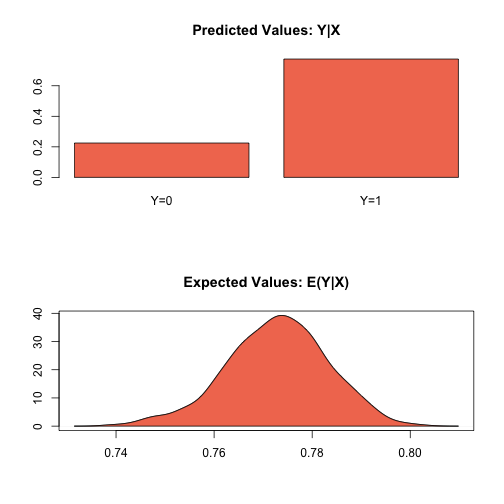
\includegraphics{unnamed-chunk-18-1.png}
\end{figure}

The cost of giving a range of values for \(\tau\) is that point
estimates are not available for quantities of interest. Instead,
quantities are presented as confidence intervals with significance less
than or equal to a specified level (e.g., at least 95\% of the
simulations are contained in the nominal 95\% confidence interval).


\subsection{Model}
\label{vignette:id53}\begin{itemize}
\item {} 
Like the standard logistic regression, the \emph{stochastic component} for
the rare events logistic regression is:
\begin{gather}
\begin{split}Y_i \; \sim \; \textrm{Bernoulli}(\pi_i),\end{split}\notag
\end{gather}
where \(Y_i\) is the binary dependent variable, and takes a value
of either 0 or 1.

\item {} 
The \emph{systematic component} is:
\begin{gather}
\begin{split}\pi_i \; = \; \frac{1}{1 + \exp(-x_i \beta)}.\end{split}\notag
\end{gather}
\item {} 
If the sample is generated via a case-control (or choice-based)
design, such as when drawing all events (or “cases”) and a sample
from the non-events (or “controls”) and going backwards to collect
the explanatory variables, you must correct for selecting on the
dependent variable. While the slope coefficients are approximately
unbiased, the constant term may be significantly biased. Zelig has
two methods for case control correction:
\begin{enumerate}
\item {} 
The “prior correction” method adjusts the intercept term. Let
\(\tau\) be the true population fraction of events,
\(\bar{y}\) the fraction of events in the sample, and
\(\hat{\beta_0}\) the uncorrected intercept term. The
corrected intercept \(\beta_0\) is:
\begin{gather}
\begin{split}\beta =  \hat{\beta_0} - \ln \left[ \bigg( \frac{1 - \tau}{\tau}
  \bigg) \bigg( \frac{\bar{y}}{1 - \bar{y}} \bigg) \right].\end{split}\notag
\end{gather}
\item {} 
The “weighting” method performs a weighted logistic regression to
correct for a case-control sampling design. Let the 1 subscript
denote observations for which the dependent variable is observed
as a 1, and the 0 subscript denote observations for which the
dependent variable is observed as a 0. Then the vector of weights
\(w_i\)
\begin{gather}
\begin{split}\begin{aligned}
w_1 &=& \frac{\tau}{\bar{y}} \\
w_0 &=& \frac{(1 - \tau)}{(1 - \bar{y})} \\
w_i &=& w_1 Y_i + w_0 (1 - Y_i)\end{aligned}\end{split}\notag
\end{gather}
\end{enumerate}

If \(\tau\) is unknown, you may alternatively specify an upper
and lower bound for the possible range of \(\tau\). In this case,
the relogit procedure uses “robust Bayesian” methods to generate a
confidence interval (rather than a point estimate) for each quantity
of interest. The nominal coverage of the confidence interval is at
least as great as the actual coverage.

\item {} 
By default, estimates of the the coefficients \(\beta\) are
bias-corrected to account for finite sample or rare events bias. In
addition, quantities of interest, such as predicted probabilities,
are also corrected of rare-events bias. If \(\widehat{\beta}\)
are the uncorrected logit coefficients and
bias(\(\widehat{\beta}\)) is the bias term, the corrected
coefficients \(\tilde{\beta}\) are
\begin{gather}
\begin{split}\widehat{\beta} - \textrm{bias}(\widehat{\beta}) = \tilde{\beta}\end{split}\notag
\end{gather}
The bias term is
\begin{gather}
\begin{split}\textrm{bias}(\widehat{\beta}) = (X'WX)^{-1} X'W \xi\end{split}\notag
\end{gather}
where
\begin{gather}
\begin{split}\begin{aligned}
\xi_i &=& 0.5 Q_{ii} \Big( (1 + w-1)\widehat{\pi}_i - w_1 \Big) \\
Q &=& X(X'WX)^{-1} X' \\
W = \textrm{diag}\{\widehat{\pi}_i (1 - \widehat{\pi}_i) w_i\}\end{aligned}\end{split}\notag
\end{gather}
where \(w_i\) and \(w_1\) are given in the “weighting”
section above.

\end{itemize}


\subsection{Quantities of Interest}
\label{vignette:id54}\begin{itemize}
\item {} 
For either one or no \(\tau\):
\begin{itemize}
\item {} 
The expected values (qi\$ev) for the rare events logit are
simulations of the predicted probability
\begin{gather}
\begin{split}E(Y) = \pi_i =
    \frac{1}{1 + \exp(-x_i \beta)},\end{split}\notag
\end{gather}
given draws of \(\beta\) from its posterior.

\item {} 
The predicted value (qi\$pr) is a draw from a binomial distribution
with mean equal to the simulated \(\pi_i\).

\item {} 
The first difference (qi\$fd) is defined as
\begin{gather}
\begin{split}\textrm{FD} = \Pr(Y = 1 \mid x_1, \tau) - \Pr(Y = 1 \mid x, \tau).\end{split}\notag
\end{gather}
\item {} 
The risk ratio (qi\$rr) is defined as
\begin{gather}
\begin{split}\textrm{RR} = \Pr(Y = 1 \mid x_1, \tau) \ / \ \Pr(Y = 1 \mid x, \tau).\end{split}\notag
\end{gather}
\end{itemize}

\item {} 
For a range of \(\tau\) defined by \([\tau_1, \tau_2]\), each
of the quantities of interest are \(n \times 2\) matrices, which
report the lower and upper bounds, respectively, for a confidence
interval with nominal coverage at least as great as the actual
coverage. At worst, these bounds are conservative estimates for the
likely range for each quantity of interest. Please refer to for the
specific method of calculating bounded quantities of interest.

\item {} 
In conditional prediction models, the average expected treatment
effect (att.ev) for the treatment group is
\begin{gather}
\begin{split}\frac{1}{\sum_{i=1}^n t_i}\sum_{i:t_i=1}^n \left\{ Y_i(t_i=1) -
      E[Y_i(t_i=0)] \right\},\end{split}\notag
\end{gather}
where \(t_i\) is a binary explanatory variable defining the
treatment (\(t_i=1\)) and control (\(t_i=0\)) groups.
Variation in the simulations are due to uncertainty in simulating
\(E[Y_i(t_i=0)]\), the counterfactual expected value of
\(Y_i\) for observations in the treatment group, under the
assumption that everything stays the same except that the treatment
indicator is switched to \(t_i=0\).

\item {} 
In conditional prediction models, the average predicted treatment
effect (att.pr) for the treatment group is
\begin{gather}
\begin{split}\frac{1}{\sum_{i=1}^n t_i}\sum_{i:t_i=1}^n \left\{ Y_i(t_i=1) -
      \widehat{Y_i(t_i=0)} \right\},\end{split}\notag
\end{gather}
where \(t_i\) is a binary explanatory variable defining the
treatment (\(t_i=1\)) and control (\(t_i=0\)) groups.
Variation in the simulations are due to uncertainty in simulating
\(\widehat{Y_i(t_i=0)}\), the counterfactual predicted value of
\(Y_i\) for observations in the treatment group, under the
assumption that everything stays the same except that the treatment
indicator is switched to \(t_i=0\).

\end{itemize}


\subsection{Output Values}
\label{vignette:id55}
The output of each Zelig command contains useful information which you
may view. For example, if you run
\code{z.out \textless{}- zelig(y \textasciitilde{} x, model = relogit, data)}, then you may examine
the available information in \code{z.out} by using \code{names(z.out)}, see
the coefficients by using z.out\$coefficients, and a default summary of
information through \code{summary(z.out)}.


\subsection{Differences with Stata Version}
\label{vignette:differences-with-stata-version}
The Stata version of ReLogit and the R implementation differ slightly in
their coefficient estimates due to differences in the matrix inversion
routines implemented in R and Stata. Zelig uses orthogonal-triangular
decomposition (through lm.influence()) to compute the bias term, which
is more numerically stable than standard matrix calculations.


\subsection{See also}
\label{vignette:id56}

\bigskip\hrule{}\bigskip



\section{zelig-tobit}
\label{vignette:zelig-tobit}\label{vignette:ztobit}
Linear Regression for a Left-Censored Dependent Variable

Tobit regression estimates a linear regression model for a left-censored
dependent variable, where the dependent variable is censored from below.
While the classical tobit model has values censored at 0, you may select
another censoring point. For other linear regression models with fully
observed dependent variables, see Bayesian regression (), maximum
likelihood normal regression (), or least squares ().


\subsection{Syntax}
\label{vignette:id57}
\begin{Verbatim}[commandchars=\\\{\}]
z5 \PYG{o}{\PYGZlt{}\PYGZhy{}} ztobit\PYG{o}{\PYGZdl{}}new\PYG{p}{(}\PYG{p}{)}
z5\PYG{o}{\PYGZdl{}}zelig\PYG{p}{(}Y \PYG{o}{\PYGZti{}} X1 \PYG{o}{+} X2\PYG{p}{,} below \PYG{o}{=} \PYG{l+m}{0}\PYG{p}{,} above \PYG{o}{=} \PYG{k+kc}{Inf}\PYG{p}{,} data \PYG{o}{=} mydata\PYG{p}{)}
z5\PYG{o}{\PYGZdl{}}setx\PYG{p}{(}\PYG{p}{)}
z5\PYG{o}{\PYGZdl{}}sim\PYG{p}{(}\PYG{p}{)}
\end{Verbatim}

With the Zelig 4 compatibility wrappers:

\begin{Verbatim}[commandchars=\\\{\}]
z.out \PYG{o}{\PYGZlt{}\PYGZhy{}} zelig\PYG{p}{(}Y \PYG{o}{\PYGZti{}} X1 \PYG{o}{+} X2\PYG{p}{,} below \PYG{o}{=} \PYG{l+m}{0}\PYG{p}{,} above \PYG{o}{=} \PYG{k+kc}{Inf}\PYG{p}{,} model \PYG{o}{=} \PYG{l+s}{\PYGZdq{}}\PYG{l+s}{tobit\PYGZdq{}}\PYG{p}{,} data \PYG{o}{=} mydata\PYG{p}{)}
x.out \PYG{o}{\PYGZlt{}\PYGZhy{}} setx\PYG{p}{(}z.out\PYG{p}{)}
s.out \PYG{o}{\PYGZlt{}\PYGZhy{}} sim\PYG{p}{(}z.out\PYG{p}{,} x \PYG{o}{=} x.out\PYG{p}{)}
\end{Verbatim}


\subsection{Inputs}
\label{vignette:inputs}
zelig() accepts the following arguments to specify how the dependent
variable is censored.
\begin{itemize}
\item {} 
\code{below}: (defaults to 0) The point at which the dependent variable
is censored from below. If any values in the dependent variable are
observed to be less than the censoring point, it is assumed that that
particular observation is censored from below at the observed value.
(See for a Bayesian implementation that supports both left and right
censoring.)

\item {} 
robust: defaults to FALSE. If TRUE, zelig() computes robust standard
errors based on sandwich estimators (see and ) and the options
selected in cluster.

\item {} 
cluster: if robust = TRUE, you may select a variable to define groups
of correlated observations. Let x3 be a variable that consists of
either discrete numeric values, character strings, or factors that
define strata. Then

\begin{Verbatim}[commandchars=\\\{\}]
\PYGZgt{} z.out \PYGZlt{}\PYGZhy{} zelig(y \PYGZti{} x1 + x2, robust = TRUE, cluster = \PYGZdq{}x3\PYGZdq{},
                 model = \PYGZdq{}tobit\PYGZdq{}, data = mydata)
\end{Verbatim}

means that the observations can be correlated within the strata
defined by the variable x3, and that robust standard errors should be
calculated according to those clusters. If robust = TRUE but cluster
is not specified, zelig() assumes that each observation falls into
its own cluster.

\end{itemize}

Zelig users may wish to refer to \code{help(survreg)} for more information.


\subsection{Examples}
\label{vignette:id58}

\subsubsection{Basic Example}
\label{vignette:id59}
Attaching the sample dataset:

\begin{Verbatim}[commandchars=\\\{\}]
data\PYG{p}{(}tobin\PYG{p}{)}
\end{Verbatim}

Estimating linear regression using \code{tobit}:

\begin{Verbatim}[commandchars=\\\{\}]
z.out \PYG{o}{\PYGZlt{}\PYGZhy{}} zelig\PYG{p}{(}durable \PYG{o}{\PYGZti{}} age \PYG{o}{+} quant\PYG{p}{,} model \PYG{o}{=} \PYG{l+s}{\PYGZdq{}}\PYG{l+s}{tobit\PYGZdq{}}\PYG{p}{,} data \PYG{o}{=} tobin\PYG{p}{)}
\end{Verbatim}

\begin{Verbatim}[commandchars=\\\{\}]
\PYG{c}{\PYGZsh{}\PYGZsh{} How to cite this model in Zelig:}
\PYG{c}{\PYGZsh{}\PYGZsh{}   Kosuke Imai, Gary King, Olivia Lau. 2011.}
\PYG{c}{\PYGZsh{}\PYGZsh{}   tobit: Linear regression for Left\PYGZhy{}Censored Dependent Variable}
\PYG{c}{\PYGZsh{}\PYGZsh{}   in Kosuke Imai, Gary King, and Olivia Lau, \PYGZdq{}Zelig: Everyone\PYGZsq{}s Statistical Software,\PYGZdq{}}
\PYG{c}{\PYGZsh{}\PYGZsh{}   http://zeligproject.org/}
\end{Verbatim}

Setting values for the explanatory variables to their sample averages:

\begin{Verbatim}[commandchars=\\\{\}]
x.out \PYG{o}{\PYGZlt{}\PYGZhy{}} setx\PYG{p}{(}z.out\PYG{p}{)}
\end{Verbatim}

Simulating quantities of interest from the posterior distribution given \code{x.out}.

\begin{Verbatim}[commandchars=\\\{\}]
s.out1 \PYG{o}{\PYGZlt{}\PYGZhy{}} sim\PYG{p}{(}z.out\PYG{p}{,} x \PYG{o}{=} x.out\PYG{p}{)}
\end{Verbatim}

\begin{Verbatim}[commandchars=\\\{\}]
summary\PYG{p}{(}s.out1\PYG{p}{)}
\end{Verbatim}

\begin{Verbatim}[commandchars=\\\{\}]
\PYG{c}{\PYGZsh{}\PYGZsh{}}
\PYG{c}{\PYGZsh{}\PYGZsh{}  sim x :}
\PYG{c}{\PYGZsh{}\PYGZsh{}  \PYGZhy{}\PYGZhy{}\PYGZhy{}\PYGZhy{}\PYGZhy{}}
\PYG{c}{\PYGZsh{}\PYGZsh{} ev}
\PYG{c}{\PYGZsh{}\PYGZsh{}       mean        sd      50\PYGZpc{}      2.5\PYGZpc{}    97.5\PYGZpc{}}
\PYG{c}{\PYGZsh{}\PYGZsh{} 1 1.522538 0.6238672 1.476463 0.4294109 2.971289}
\PYG{c}{\PYGZsh{}\PYGZsh{} pv}
\PYG{c}{\PYGZsh{}\PYGZsh{}         mean       sd      50\PYGZpc{} 2.5\PYGZpc{}    97.5\PYGZpc{}}
\PYG{c}{\PYGZsh{}\PYGZsh{} [1,] 3.09644 3.898018 1.431842    0 12.69079}
\end{Verbatim}


\subsubsection{Simulating First Differences}
\label{vignette:id60}
Set explanatory variables to their default(mean/mode) values, with
high (80th percentile) and low (20th percentile) liquidity ratio
(\code{quant}):

\begin{Verbatim}[commandchars=\\\{\}]
x.high \PYG{o}{\PYGZlt{}\PYGZhy{}} setx\PYG{p}{(}z.out\PYG{p}{,} quant \PYG{o}{=} quantile\PYG{p}{(}tobin\PYG{o}{\PYGZdl{}}quant\PYG{p}{,} prob \PYG{o}{=} \PYG{l+m}{0.8}\PYG{p}{)}\PYG{p}{)}
x.low \PYG{o}{\PYGZlt{}\PYGZhy{}} setx\PYG{p}{(}z.out\PYG{p}{,} quant \PYG{o}{=} quantile\PYG{p}{(}tobin\PYG{o}{\PYGZdl{}}quant\PYG{p}{,} prob \PYG{o}{=} \PYG{l+m}{0.2}\PYG{p}{)}\PYG{p}{)}
\end{Verbatim}

Estimating the first difference for the effect of high versus low
liquidity ratio on duration(\code{durable}):

\begin{Verbatim}[commandchars=\\\{\}]
s.out2 \PYG{o}{\PYGZlt{}\PYGZhy{}} sim\PYG{p}{(}z.out\PYG{p}{,} x \PYG{o}{=} x.high\PYG{p}{,} x1 \PYG{o}{=} x.low\PYG{p}{)}
\end{Verbatim}

\begin{Verbatim}[commandchars=\\\{\}]
summary\PYG{p}{(}s.out2\PYG{p}{)}
\end{Verbatim}

\begin{Verbatim}[commandchars=\\\{\}]
\PYG{c}{\PYGZsh{}\PYGZsh{}}
\PYG{c}{\PYGZsh{}\PYGZsh{}  sim x :}
\PYG{c}{\PYGZsh{}\PYGZsh{}  \PYGZhy{}\PYGZhy{}\PYGZhy{}\PYGZhy{}\PYGZhy{}}
\PYG{c}{\PYGZsh{}\PYGZsh{} ev}
\PYG{c}{\PYGZsh{}\PYGZsh{}       mean        sd      50\PYGZpc{}     2.5\PYGZpc{}   97.5\PYGZpc{}}
\PYG{c}{\PYGZsh{}\PYGZsh{} 1 1.192813 0.7800701 1.070859 0.123258 3.16135}
\PYG{c}{\PYGZsh{}\PYGZsh{} pv}
\PYG{c}{\PYGZsh{}\PYGZsh{}          mean       sd      50\PYGZpc{} 2.5\PYGZpc{}    97.5\PYGZpc{}}
\PYG{c}{\PYGZsh{}\PYGZsh{} [1,] 3.132773 4.150502 1.323289    0 14.14609}
\PYG{c}{\PYGZsh{}\PYGZsh{}}
\PYG{c}{\PYGZsh{}\PYGZsh{}  sim x1 :}
\PYG{c}{\PYGZsh{}\PYGZsh{}  \PYGZhy{}\PYGZhy{}\PYGZhy{}\PYGZhy{}\PYGZhy{}}
\PYG{c}{\PYGZsh{}\PYGZsh{} ev}
\PYG{c}{\PYGZsh{}\PYGZsh{}       mean        sd      50\PYGZpc{}      2.5\PYGZpc{}    97.5\PYGZpc{}}
\PYG{c}{\PYGZsh{}\PYGZsh{} 1 2.023184 0.9289575 1.907224 0.5365063 4.132607}
\PYG{c}{\PYGZsh{}\PYGZsh{} pv}
\PYG{c}{\PYGZsh{}\PYGZsh{}          mean       sd     50\PYGZpc{} 2.5\PYGZpc{}    97.5\PYGZpc{}}
\PYG{c}{\PYGZsh{}\PYGZsh{} [1,] 3.724101 4.401357 2.11134    0 15.06014}
\PYG{c}{\PYGZsh{}\PYGZsh{} fd}
\PYG{c}{\PYGZsh{}\PYGZsh{}        mean       sd       50\PYGZpc{}      2.5\PYGZpc{}    97.5\PYGZpc{}}
\PYG{c}{\PYGZsh{}\PYGZsh{} 1 0.8303709 1.143904 0.7664756 \PYGZhy{}1.441829 3.200998}
\end{Verbatim}

\begin{Verbatim}[commandchars=\\\{\}]
plot\PYG{p}{(}s.out1\PYG{p}{)}
\end{Verbatim}
\begin{figure}[htbp]
\centering
\capstart

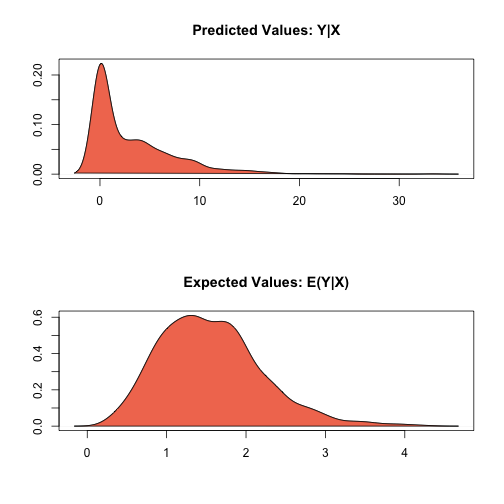
\includegraphics{Zelig-tobit-1.png}
\caption{Zelig-tobit}\end{figure}


\subsection{Model}
\label{vignette:id61}\begin{itemize}
\item {} 
Let \(Y_i^*\) be a latent dependent variable which is distributed
with \emph{stochastic} component
\begin{gather}
\begin{split}\begin{aligned}
Y_i^* & \sim & \textrm{Normal}(\mu_i, \sigma^2) \\\end{aligned}\end{split}\notag
\end{gather}
where \(\mu_i\) is a vector means and \(\sigma^2\) is a
scalar variance parameter. \(Y_i^*\) is not directly observed,
however. Rather we observed \(Y_i\) which is defined as:
\begin{gather}
\begin{split}Y_i = \left\{
\begin{array}{lcl}
Y_i^*  &\textrm{if} & c <Y_i^* \\
c    &\textrm{if} & c \ge Y_i^*
\end{array}\right.\end{split}\notag
\end{gather}
where \(c\) is the lower bound below which \(Y_i^*\) is
censored.

\item {} 
The \emph{systematic component} is given by
\begin{gather}
\begin{split}\begin{aligned}
\mu_{i} &=& x_{i} \beta,\end{aligned}\end{split}\notag
\end{gather}
where \(x_{i}\) is the vector of \(k\) explanatory variables
for observation \(i\) and \(\beta\) is the vector of
coefficients.

\end{itemize}


\subsection{Quantities of Interest}
\label{vignette:id62}\begin{itemize}
\item {} 
The expected values (\code{qi\$ev}) for the tobit regression model are
the same as the expected value of \(Y*\):
\begin{gather}
\begin{split}E(Y^* | X) = \mu_{i} = x_{i} \beta\end{split}\notag
\end{gather}
\item {} 
The first difference (\code{qi\$fd}) for the tobit regression model is
defined as
\begin{gather}
\begin{split}\begin{aligned}
\text{FD}=E(Y^* \mid x_{1}) - E(Y^* \mid x).\end{aligned}\end{split}\notag
\end{gather}
\item {} 
In conditional prediction models, the average expected treatment
effect (\code{qi\$att.ev}) for the treatment group is
\begin{gather}
\begin{split}\begin{aligned}
\frac{1}{\sum t_{i}}\sum_{i:t_{i}=1}[E[Y^*_{i}(t_{i}=1)]-E[Y^*_{i}(t_{i}=0)]],\end{aligned}\end{split}\notag
\end{gather}
where \(t_{i}\) is a binary explanatory variable defining the
treatment (\(t_{i}=1\)) and control (\(t_{i}=0\)) groups.

\end{itemize}


\subsection{Output Values}
\label{vignette:id63}
The output of each Zelig command contains useful information which you
may view. For example, if you run:

\begin{Verbatim}[commandchars=\\\{\}]
z.out \PYG{o}{\PYGZlt{}\PYGZhy{}} zelig\PYG{p}{(}y \PYG{o}{\PYGZti{}} x\PYG{p}{,} model \PYG{o}{=} \PYG{l+s}{\PYGZdq{}}\PYG{l+s}{tobit\PYGZdq{}}\PYG{p}{,} data\PYG{p}{)}
\end{Verbatim}

then you may examine the available information in {\color{red}\bfseries{}{}`{}`}z.out{}`.


\subsection{See also}
\label{vignette:id66}
The tobit function is part of the survival library by Terry Therneau,
ported to R by Thomas Lumley. Advanced users may wish to refer to
\code{help(survfit)} in the survival library.


\bigskip\hrule{}\bigskip



\section{zelig-factorbayes}
\label{vignette:zelig-factorbayes}\label{vignette:zfactorbayes}
Given some unobserved explanatory variables and observed dependent
variables, the Normal theory factor analysis model estimates the latent
factors. The model is implemented using a Markov Chain Monte Carlo
algorithm (Gibbs sampling with data augmentation). For factor analysis
with ordinal dependent variables, see ordered factor analysis (), and
for a mix of types of dependent variables, see the mixed factor analysis
model ().


\subsection{Syntax}
\label{vignette:id67}
With reference classes:

\begin{Verbatim}[commandchars=\\\{\}]
z5 \PYG{o}{\PYGZlt{}\PYGZhy{}} zfactorbayes\PYG{o}{\PYGZdl{}}new\PYG{p}{(}\PYG{p}{)}
z5\PYG{o}{\PYGZdl{}}zelig\PYG{p}{(}cbind\PYG{p}{(}Y1 \PYG{p}{,}Y2\PYG{p}{,} Y3\PYG{p}{)} \PYG{o}{\PYGZti{}} \PYG{k+kc}{NULL}\PYG{p}{,} factors \PYG{o}{=} \PYG{l+m}{2}\PYG{p}{,}
         model \PYG{o}{=} \PYG{l+s}{\PYGZdq{}}\PYG{l+s}{factor.bayes\PYGZdq{}}\PYG{p}{,} data \PYG{o}{=} mydata\PYG{p}{)}
\end{Verbatim}

With the Zelig 4 compatibility wrappers:

\begin{Verbatim}[commandchars=\\\{\}]
z.out \PYG{o}{\PYGZlt{}\PYGZhy{}} zelig\PYG{p}{(}cbind\PYG{p}{(}Y1 \PYG{p}{,}Y2\PYG{p}{,} Y3\PYG{p}{)} \PYG{o}{\PYGZti{}} \PYG{k+kc}{NULL}\PYG{p}{,} factors \PYG{o}{=} \PYG{l+m}{2}\PYG{p}{,}
               model \PYG{o}{=} \PYG{l+s}{\PYGZdq{}}\PYG{l+s}{factor.bayes\PYGZdq{}}\PYG{p}{,} data \PYG{o}{=} mydata\PYG{p}{)}
\end{Verbatim}


\subsection{Inputs}
\label{vignette:id68}
zelig() takes the following functions for factor.bayes:
\begin{itemize}
\item {} 
\code{Y1}, \code{Y2}, and \code{Y3}: variables of interest in factor analysis
(manifest variables), assumed to be normally distributed. The model
requires a minimum of three manifest variables.

\item {} 
\code{factors}: number of the factors to be fitted (defaults to 2).

\end{itemize}


\subsection{Additional Inputs}
\label{vignette:additional-inputs}
In addition, zelig() accepts the following additional arguments for
model specification:
\begin{itemize}
\item {} 
\code{lambda.constraints}: list containing the equality or inequality
constraints on the factor loadings. Choose from one of the following
forms:
\begin{itemize}
\item {} 
varname = list(): by default, no constraints are imposed.

\item {} 
\code{varname = list(d, c)}: constrains the \(d\)th loading for
the variable named \code{varname} to be equal to \code{c}.

\item {} 
\code{varname = list(d, +)}: constrains the \(d\)th loading for
the variable named \code{varname} to be positive;

\item {} 
\code{varname = list(d, -)}: constrains the \(d\)th loading for
the variable named \code{varname} to be negative.

\end{itemize}

\item {} 
\code{std.var}: defaults to FALSE (manifest variables are rescaled to
zero mean, but retain observed variance). If \code{TRUE}, the manifest
variables are rescaled to be mean zero and unit variance.

\end{itemize}

In addition, zelig() accepts the following additional inputs for
bayes.factor:
\begin{itemize}
\item {} 
\code{burnin}: number of the initial MCMC iterations to be discarded
(defaults to 1,000).

\item {} 
\code{mcmc}: number of the MCMC iterations after burnin (defaults to
20,000).

\item {} 
\code{thin}: thinning interval for the Markov chain. Only every
\code{thin}-th draw from the Markov chain is kept. The value of \code{mcmc}
must be divisible by this value. The default value is 1.

\item {} 
\code{verbose}: defaults to FALSE. If \code{TRUE}, the progress of the
sampler (every \(10\%\)) is printed to the screen.

\item {} 
\code{seed}: seed for the random number generator. The default is \code{NA}
which corresponds to a random seed 12345.

\item {} 
\code{Lambda.start}: starting values of the factor loading matrix
\(\Lambda\), either a scalar (all unconstrained loadings are set
to that value), or a matrix with compatible dimensions. The default
is \code{NA}, where the start value are set to be 0 for unconstrained
factor loadings, and 0.5 or \(-\)0.5 for constrained factor
loadings (depending on the nature of the constraints).

\item {} 
\code{Psi.start}: starting values for the uniquenesses, either a scalar
(the starting values for all diagonal elements of \(\Psi\) are
set to be this value), or a vector with length equal to the number of
manifest variables. In the latter case, the starting values of the
diagonal elements of \(\Psi\) take the values of \code{Psi.start}.
The default value is \code{NA} where the starting values of the all the
uniquenesses are set to be 0.5.

\item {} 
\code{store.lambda}: defaults to TRUE, which stores the posterior draws
of the factor loadings.

\item {} 
\code{store.scores}: defaults to FALSE. If TRUE, stores the posterior
draws of the factor scores. (Storing factor scores may take large
amount of memory for a large number of draws or observations.)

\end{itemize}

The model also accepts the following additional arguments to specify
prior parameters:
\begin{itemize}
\item {} 
\code{l0}: mean of the Normal prior for the factor loadings, either a
scalar or a matrix with the same dimensions as \(\Lambda\). If a
scalar value, that value will be the prior mean for all the factor
loadings. Defaults to 0.

\item {} 
\code{L0}: precision parameter of the Normal prior for the factor
loadings, either a scalar or a matrix with the same dimensions as
\(\Lambda\). If \code{L0} takes a scalar value, then the precision
matrix will be a diagonal matrix with the diagonal elements set to
that value. The default value is 0, which leads to an improper prior.

\item {} 
\code{a0}: the shape parameter of the Inverse Gamma prior for the
uniquenesses is \code{a0/2}. It can take a scalar value or a vector. The
default value is 0.001.

\item {} 
\code{b0}: the shape parameter of the Inverse Gamma prior for the
uniquenesses is \code{b0/2}. It can take a scalar value or a vector. The
default value is 0.001.

\end{itemize}

Zelig users may wish to refer to \code{help(MCMCfactanal)} for more
information.


\subsection{Example}
\label{vignette:id69}
Attaching the sample dataset:

\begin{Verbatim}[commandchars=\\\{\}]
data\PYG{p}{(}swiss\PYG{p}{)}
names\PYG{p}{(}swiss\PYG{p}{)} \PYG{o}{\PYGZlt{}\PYGZhy{}} c\PYG{p}{(}\PYG{l+s}{\PYGZdq{}}\PYG{l+s}{Fert\PYGZdq{}}\PYG{p}{,} \PYG{l+s}{\PYGZdq{}}\PYG{l+s}{Agr\PYGZdq{}}\PYG{p}{,} \PYG{l+s}{\PYGZdq{}}\PYG{l+s}{Exam\PYGZdq{}}\PYG{p}{,} \PYG{l+s}{\PYGZdq{}}\PYG{l+s}{Educ\PYGZdq{}}\PYG{p}{,} \PYG{l+s}{\PYGZdq{}}\PYG{l+s}{Cath\PYGZdq{}}\PYG{p}{,} \PYG{l+s}{\PYGZdq{}}\PYG{l+s}{InfMort\PYGZdq{}}\PYG{p}{)}
\end{Verbatim}

Factor analysis:

\begin{Verbatim}[commandchars=\\\{\}]
z.out \PYG{o}{\PYGZlt{}\PYGZhy{}} zelig\PYG{p}{(}cbind\PYG{p}{(}Agr\PYG{p}{,} Exam\PYG{p}{,} Educ\PYG{p}{,} Cath\PYG{p}{,} InfMort\PYG{p}{)} \PYG{o}{\PYGZti{}} \PYG{k+kc}{NULL}\PYG{p}{,}
               model \PYG{o}{=} \PYG{l+s}{\PYGZdq{}}\PYG{l+s}{factor.bayes\PYGZdq{}}\PYG{p}{,} data \PYG{o}{=} swiss\PYG{p}{,} factors \PYG{o}{=} \PYG{l+m}{2}\PYG{p}{,} verbose \PYG{o}{=} \PYG{k+kc}{TRUE}\PYG{p}{,}
               a0 \PYG{o}{=} \PYG{l+m}{1}\PYG{p}{,} b0 \PYG{o}{=} \PYG{l+m}{0.15}\PYG{p}{,} burnin \PYG{o}{=} \PYG{l+m}{5000}\PYG{p}{,} mcmc \PYG{o}{=} \PYG{l+m}{50000}\PYG{p}{)}
\end{Verbatim}

Checking for convergence before summarizing the estimates:

\begin{Verbatim}[commandchars=\\\{\}]
algor \PYG{o}{\PYGZlt{}\PYGZhy{}} try\PYG{p}{(}geweke.diag\PYG{p}{(}z.out\PYG{o}{\PYGZdl{}}coefficients\PYG{p}{)}\PYG{p}{,} silent\PYG{o}{=}\PYG{k+kVariable}{T}\PYG{p}{)}
\PYG{k+kr}{if} \PYG{p}{(}class\PYG{p}{(}algor\PYG{p}{)} \PYG{o}{==} \PYG{l+s}{\PYGZdq{}}\PYG{l+s}{try\PYGZhy{}error\PYGZdq{}}\PYG{p}{)}
    print\PYG{p}{(}algor\PYG{p}{)}
\end{Verbatim}

Since the algorithm did not converge, we now add some constraints on
\(\Lambda\) to optimize the algorithm:

\begin{Verbatim}[commandchars=\\\{\}]
z.out \PYG{o}{\PYGZlt{}\PYGZhy{}} zelig\PYG{p}{(}cbind\PYG{p}{(}Agr\PYG{p}{,} Exam\PYG{p}{,} Educ\PYG{p}{,} Cath\PYG{p}{,} InfMort\PYG{p}{)} \PYG{o}{\PYGZti{}} \PYG{k+kc}{NULL}\PYG{p}{,}
               model \PYG{o}{=} \PYG{l+s}{\PYGZdq{}}\PYG{l+s}{factor.bayes\PYGZdq{}}\PYG{p}{,} data \PYG{o}{=} swiss\PYG{p}{,} factors \PYG{o}{=} \PYG{l+m}{2}\PYG{p}{,}
               lambda.constraints \PYG{o}{=} list\PYG{p}{(}Exam \PYG{o}{=} list\PYG{p}{(}\PYG{l+m}{1}\PYG{p}{,}\PYG{l+s}{\PYGZdq{}}\PYG{l+s}{+\PYGZdq{}}\PYG{p}{)}\PYG{p}{,}
                   Exam \PYG{o}{=} list\PYG{p}{(}\PYG{l+m}{2}\PYG{p}{,}\PYG{l+s}{\PYGZdq{}}\PYG{l+s}{\PYGZhy{}\PYGZdq{}}\PYG{p}{)}\PYG{p}{,} Educ \PYG{o}{=} c\PYG{p}{(}\PYG{l+m}{2}\PYG{p}{,} \PYG{l+m}{0}\PYG{p}{)}\PYG{p}{,}
                   InfMort \PYG{o}{=} c\PYG{p}{(}\PYG{l+m}{1}\PYG{p}{,} \PYG{l+m}{0}\PYG{p}{)}\PYG{p}{)}\PYG{p}{,}
               verbose \PYG{o}{=} \PYG{k+kc}{TRUE}\PYG{p}{,} a0 \PYG{o}{=} \PYG{l+m}{1}\PYG{p}{,} b0 \PYG{o}{=} \PYG{l+m}{0.15}\PYG{p}{,}
               burnin \PYG{o}{=} \PYG{l+m}{5000}\PYG{p}{,} mcmc \PYG{o}{=} \PYG{l+m}{50000}\PYG{p}{)}
geweke.diag\PYG{p}{(}z.out\PYG{o}{\PYGZdl{}}coefficients\PYG{p}{)}
heidel.diag\PYG{p}{(}z.out\PYG{o}{\PYGZdl{}}coefficients\PYG{p}{)}
raftery.diag\PYG{p}{(}z.out\PYG{o}{\PYGZdl{}}coefficients\PYG{p}{)}
summary\PYG{p}{(}z.out\PYG{p}{)}
\end{Verbatim}


\subsection{Model}
\label{vignette:id70}
Suppose for observation \(i\) we observe \(K\) variables and
hypothesize that there are \(d\) underlying factors such that:
\begin{gather}
\begin{split}\begin{aligned}
Y_i = \Lambda \phi_i+\epsilon_i\end{aligned}\end{split}\notag
\end{gather}
where \(Y_{i}\) is the vector of \(K\) manifest variables for
observation \(i\). \(\Lambda\) is the \(K \times d\) factor
loading matrix and \(\phi_i\) is the \(d\)-vector of latent
factor scores. Both \(\Lambda\) and \(\phi\) need to be
estimated.
\begin{itemize}
\item {} 
The \emph{stochastic component} is given by:
\begin{gather}
\begin{split}\begin{aligned}
\epsilon_{i}  \sim \textrm{Normal}(0, \Psi).\end{aligned}\end{split}\notag
\end{gather}
where \(\Psi\) is a diagonal, positive definite matrix. The
diagonal elements of \(\Psi\) are referred to as uniquenesses.

\item {} 
The \emph{systematic component} is given by
\begin{gather}
\begin{split}\begin{aligned}
\mu_i = E(Y_i) = \Lambda\phi_i\end{aligned}\end{split}\notag
\end{gather}
\item {} 
The independent conjugate \emph{prior} for each \(\Lambda_{ij}\) is
given by
\begin{gather}
\begin{split}\begin{aligned}
\Lambda_{ij} \sim \textrm{Normal}(l_{0_{ij}}, L_{0_{ij}}^{-1})
\textrm{ for } i=1,\ldots, k; \quad j=1,\ldots, d. \end{aligned}\end{split}\notag
\end{gather}
\item {} 
The independent conjugate \emph{prior} for each \(\Psi_{ii}\) is given
by
\begin{gather}
\begin{split}\begin{aligned}
\Psi_{ii} \sim \textrm{InverseGamma}(\frac{a_0}{2}, \frac{b_0}{2}), \textrm{ for }
i = 1, \ldots, k.\end{aligned}\end{split}\notag
\end{gather}
\item {} 
The \emph{prior} for \(\phi_i\) is
\begin{gather}
\begin{split}\begin{aligned}
\phi_i &\sim& \textrm{Normal}(0, I_d), \textrm{ for } i = 1, \ldots, n.\end{aligned}\end{split}\notag
\end{gather}
where \(I_d\) is a :math:{}` dtimes d {}` identity matrix.

\end{itemize}


\subsection{Output Values}
\label{vignette:id71}
The output of each Zelig command contains useful information which you
may view. For example, if you run:

\begin{Verbatim}[commandchars=\\\{\}]
z.out \PYG{o}{\PYGZlt{}\PYGZhy{}} zelig\PYG{p}{(}cbind\PYG{p}{(}Y1\PYG{p}{,} Y2\PYG{p}{,} Y3\PYG{p}{)}\PYG{p}{,} model \PYG{o}{=} \PYG{l+s}{\PYGZdq{}}\PYG{l+s}{factor.bayes\PYGZdq{}}\PYG{p}{,} data\PYG{p}{)}
\end{Verbatim}

then you may examine the available information in \code{z.out} by using
\code{names(z.out)}, see the draws from the posterior distribution of the
\code{coefficients} by using \code{z.out\$coefficients}, and view a default
summary of information through \code{summary(z.out)}. Other elements
available through the \code{\$} operator are listed below.
\begin{itemize}
\item {} 
From the \code{zelig()} output object \code{z.out}, you may extract:
\begin{itemize}
\item {} 
\code{coefficients}: draws from the posterior distributions of the
estimated factor loadings and the uniquenesses. If
\code{store.scores = TRUE}, the estimated factors scores are also
contained in \code{coefficients}.

\item {} 
\code{data}: the name of the input data frame.

\item {} 
\code{seed}: the random seed used in the model.

\end{itemize}

\item {} 
Since there are no explanatory variables, the \code{sim()} procedure is
not applicable for factor analysis models.

\end{itemize}


\bigskip\hrule{}\bigskip



\section{zelig-mlogitbayes}
\label{vignette:zelig-mlogitbayes}\label{vignette:zmlogitbayes}
Use Bayesian multinomial logistic regression to model unordered
categorical variables. The dependent variable may be in the format of
either character strings or integer values. The model is estimated via a
random walk Metropolis algorithm or a slice sampler. See for the
maximum-likelihood estimation of this model.


\subsection{Syntax}
\label{vignette:id72}
With reference classes:

\begin{Verbatim}[commandchars=\\\{\}]
z5 \PYG{o}{\PYGZlt{}\PYGZhy{}} zmlogitbayes\PYG{o}{\PYGZdl{}}new\PYG{p}{(}\PYG{p}{)}
z5\PYG{o}{\PYGZdl{}}zelig\PYG{p}{(}Y \PYG{o}{\PYGZti{}} X1 \PYG{o}{+} X2\PYG{p}{,} data \PYG{o}{=} mydata\PYG{p}{)}
z5\PYG{o}{\PYGZdl{}}setx\PYG{p}{(}\PYG{p}{)}
z5\PYG{o}{\PYGZdl{}}sim\PYG{p}{(}\PYG{p}{)}
\end{Verbatim}

With the Zelig 4 compatibility wrappers:

\begin{Verbatim}[commandchars=\\\{\}]
z.out \PYG{o}{\PYGZlt{}\PYGZhy{}} zelig\PYG{p}{(}Y \PYG{o}{\PYGZti{}} X1 \PYG{o}{+} X2\PYG{p}{,} model \PYG{o}{=} \PYG{l+s}{\PYGZdq{}}\PYG{l+s}{mlogit.bayes\PYGZdq{}}\PYG{p}{,} data \PYG{o}{=} mydata\PYG{p}{)}
x.out \PYG{o}{\PYGZlt{}\PYGZhy{}} setx\PYG{p}{(}z.out\PYG{p}{)}
s.out \PYG{o}{\PYGZlt{}\PYGZhy{}} sim\PYG{p}{(}z.out\PYG{p}{,} x \PYG{o}{=} x.out\PYG{p}{)}
\end{Verbatim}


\subsection{Additional Inputs}
\label{vignette:id73}
zelig() accepts the following arguments for mlogit.bayes:
\begin{itemize}
\item {} 
\code{baseline}: either a character string or numeric value (equal to
one of the observed values in the dependent variable) specifying a
baseline category. The default value is \code{NA} which sets the
baseline to the first alphabetical or numerical unique value of the
dependent variable.

\end{itemize}

The model accepts the following additional arguments to monitor the
Markov chains:
\begin{itemize}
\item {} 
\code{burnin}: number of the initial MCMC iterations to be discarded
(defaults to 1,000).

\item {} 
\code{mcmc}: number of the MCMC iterations after burnin (defaults to
10,000).

\item {} 
\code{thin}: thinning interval for the Markov chain. Only every
\code{thin}-th draw from the Markov chain is kept. The value of \code{mcmc}
must be divisible by this value. The default value is 1.

\item {} 
\code{mcmc.method}: either “MH” or “slice”, specifying whether to use
Metropolis Algorithm or slice sampler. The default value is \code{MH}.

\item {} 
\code{tune}: tuning parameter for the Metropolis-Hasting step, either a
scalar or a numeric vector (for \(k\) coefficients, enter a
\(k\) vector). The tuning parameter should be set such that the
acceptance rate is satisfactory (between 0.2 and 0.5). The default
value is 1.1.

\item {} 
\code{verbose}: defaults to \code{FALSE}. If \code{TRUE}, the progress of the
sampler (every \(10\%\)) is printed to the screen.

\item {} 
\code{seed}: seed for the random number generator. The default is \code{NA}
which corresponds to a random seed of 12345.

\item {} 
\code{beta.start}: starting values for the Markov chain, either a scalar
or a vector (for \(k\) coefficients, enter a \(k\) vector).
The default is \code{NA} where the maximum likelihood estimates are used
as the starting values.

\end{itemize}

Use the following arguments to specify the priors for the model:
\begin{itemize}
\item {} 
\code{b0}: prior mean for the coefficients, either a scalar or vector.
If a scalar, that value will be the prior mean for all the
coefficients. The default is 0.

\item {} 
\code{B0}: prior precision parameter for the coefficients, either a
square matrix with the dimensions equal to the number of coefficients
or a scalar. If a scalar, that value times an identity matrix will be
the prior precision parameter. The default is 0 which leads to an
improper prior.

\end{itemize}

Zelig users may wish to refer to \code{help(MCMCmnl)} for more information.


\subsection{Examples}
\label{vignette:id74}

\subsubsection{Basic Example}
\label{vignette:id75}
Attaching the sample dataset:

\begin{Verbatim}[commandchars=\\\{\}]
data\PYG{p}{(}mexico\PYG{p}{)}
\end{Verbatim}

Estimating multinomial logistics regression using \code{mlogit.bayes}:

\begin{Verbatim}[commandchars=\\\{\}]
z.out \PYG{o}{\PYGZlt{}\PYGZhy{}} zelig\PYG{p}{(}vote88 \PYG{o}{\PYGZti{}} pristr \PYG{o}{+} othcok \PYG{o}{+} othsocok\PYG{p}{,}
               model \PYG{o}{=} \PYG{l+s}{\PYGZdq{}}\PYG{l+s}{mlogit.bayes\PYGZdq{}}\PYG{p}{,} data \PYG{o}{=} mexico\PYG{p}{,}
               verbose \PYG{o}{=} \PYG{k+kc}{FALSE}\PYG{p}{)}
\end{Verbatim}

\begin{Verbatim}[commandchars=\\\{\}]
\PYG{c}{\PYGZsh{}\PYGZsh{} Calculating MLEs and large sample var\PYGZhy{}cov matrix.}
\PYG{c}{\PYGZsh{}\PYGZsh{} This may take a moment...}
\PYG{c}{\PYGZsh{}\PYGZsh{} Inverting Hessian to get large sample var\PYGZhy{}cov matrix.}
\end{Verbatim}

\begin{Verbatim}[commandchars=\\\{\}]
\PYG{c}{\PYGZsh{}\PYGZsh{} Warning in if (mcmc.method == \PYGZdq{}RWM\PYGZdq{}) \PYGZob{}: the condition has length \PYGZgt{} 1 and}
\PYG{c}{\PYGZsh{}\PYGZsh{} only the first element will be used}
\end{Verbatim}

\begin{Verbatim}[commandchars=\\\{\}]
\PYG{c}{\PYGZsh{}\PYGZsh{} Warning in if (mcmc.method == \PYGZdq{}IndMH\PYGZdq{}) \PYGZob{}: the condition has length \PYGZgt{} 1 and}
\PYG{c}{\PYGZsh{}\PYGZsh{} only the first element will be used}
\end{Verbatim}

\begin{Verbatim}[commandchars=\\\{\}]
\PYG{c}{\PYGZsh{}\PYGZsh{} How to cite this model in Zelig:}
\PYG{c}{\PYGZsh{}\PYGZsh{}   Ben Goodrich, Ying Lu. 2013.}
\PYG{c}{\PYGZsh{}\PYGZsh{}   mlogitbayes: Bayesian Multinomial Logistic Regression for Dependent Variables with Unordered Categorical Values}
\PYG{c}{\PYGZsh{}\PYGZsh{}   in Kosuke Imai, Gary King, and Olivia Lau, \PYGZdq{}Zelig: Everyone\PYGZsq{}s Statistical Software,\PYGZdq{}}
\PYG{c}{\PYGZsh{}\PYGZsh{}   http://zeligproject.org/}
\end{Verbatim}

Checking for convergence before summarizing the estimates:

\begin{Verbatim}[commandchars=\\\{\}]
raftery.diag\PYG{p}{(}z.out\PYG{o}{\PYGZdl{}}coefficients\PYG{p}{)}
\end{Verbatim}

\begin{Verbatim}[commandchars=\\\{\}]
summary\PYG{p}{(}z.out\PYG{p}{)}
\end{Verbatim}

Setting values for the explanatory variables to their sample
averages:

\begin{Verbatim}[commandchars=\\\{\}]
x.out \PYG{o}{\PYGZlt{}\PYGZhy{}} setx\PYG{p}{(}z.out\PYG{p}{)}
\end{Verbatim}

Simulating quantities of interest from the posterior distribution
given \code{x.out}.

\begin{Verbatim}[commandchars=\\\{\}]
s.out1 \PYG{o}{\PYGZlt{}\PYGZhy{}} sim\PYG{p}{(}z.out\PYG{p}{,} x \PYG{o}{=} x.out\PYG{p}{)}
summary\PYG{p}{(}s.out1\PYG{p}{)}
\end{Verbatim}

\begin{Verbatim}[commandchars=\\\{\}]
\PYG{c}{\PYGZsh{}\PYGZsh{}}
\PYG{c}{\PYGZsh{}\PYGZsh{}  sim x :}
\PYG{c}{\PYGZsh{}\PYGZsh{}  \PYGZhy{}\PYGZhy{}\PYGZhy{}\PYGZhy{}\PYGZhy{}}
\PYG{c}{\PYGZsh{}\PYGZsh{} ev}
\PYG{c}{\PYGZsh{}\PYGZsh{}             mean         sd       50\PYGZpc{}      2.5\PYGZpc{}     97.5\PYGZpc{}}
\PYG{c}{\PYGZsh{}\PYGZsh{} P(Y=1) 0.5613368 0.01592425 0.5615034 0.5306640 0.5914963}
\PYG{c}{\PYGZsh{}\PYGZsh{} P(Y=2) 0.2099124 0.01273148 0.2098424 0.1854312 0.2350891}
\PYG{c}{\PYGZsh{}\PYGZsh{} P(Y=3) 0.2287508 0.01360126 0.2285987 0.2033590 0.2558153}
\PYG{c}{\PYGZsh{}\PYGZsh{} pv}
\PYG{c}{\PYGZsh{}\PYGZsh{} qi}
\PYG{c}{\PYGZsh{}\PYGZsh{}      1      2      3}
\PYG{c}{\PYGZsh{}\PYGZsh{} 0.5544 0.2155 0.2301}
\end{Verbatim}


\subsubsection{Simulating First Differences}
\label{vignette:id76}
Estimating the first difference (and risk ratio) in the
probabilities of voting different candidates when \code{pristr} (the
strength of the PRI) is set to be weak (equal to 1) versus strong
(equal to 3) while all the other variables held at their default
values.

\begin{Verbatim}[commandchars=\\\{\}]
x.weak \PYG{o}{\PYGZlt{}\PYGZhy{}} setx\PYG{p}{(}z.out\PYG{p}{,} pristr \PYG{o}{=} \PYG{l+m}{1}\PYG{p}{)}
x.strong \PYG{o}{\PYGZlt{}\PYGZhy{}} setx\PYG{p}{(}z.out\PYG{p}{,} pristr \PYG{o}{=} \PYG{l+m}{3}\PYG{p}{)}
s.out2 \PYG{o}{\PYGZlt{}\PYGZhy{}} sim\PYG{p}{(}z.out\PYG{p}{,} x \PYG{o}{=} x.strong\PYG{p}{,} x1 \PYG{o}{=} x.weak\PYG{p}{)}
summary\PYG{p}{(}s.out2\PYG{p}{)}
\end{Verbatim}

\begin{Verbatim}[commandchars=\\\{\}]
\PYG{c}{\PYGZsh{}\PYGZsh{}}
\PYG{c}{\PYGZsh{}\PYGZsh{}  sim x :}
\PYG{c}{\PYGZsh{}\PYGZsh{}  \PYGZhy{}\PYGZhy{}\PYGZhy{}\PYGZhy{}\PYGZhy{}}
\PYG{c}{\PYGZsh{}\PYGZsh{} ev}
\PYG{c}{\PYGZsh{}\PYGZsh{}             mean         sd       50\PYGZpc{}      2.5\PYGZpc{}     97.5\PYGZpc{}}
\PYG{c}{\PYGZsh{}\PYGZsh{} P(Y=1) 0.7156880 0.02127842 0.7158103 0.6725681 0.7561260}
\PYG{c}{\PYGZsh{}\PYGZsh{} P(Y=2) 0.1270237 0.01458077 0.1265905 0.1000858 0.1562571}
\PYG{c}{\PYGZsh{}\PYGZsh{} P(Y=3) 0.1572883 0.01646202 0.1568142 0.1260809 0.1909916}
\PYG{c}{\PYGZsh{}\PYGZsh{} pv}
\PYG{c}{\PYGZsh{}\PYGZsh{} qi}
\PYG{c}{\PYGZsh{}\PYGZsh{}      1      2      3}
\PYG{c}{\PYGZsh{}\PYGZsh{} 0.7241 0.1153 0.1606}
\PYG{c}{\PYGZsh{}\PYGZsh{}}
\PYG{c}{\PYGZsh{}\PYGZsh{}  sim x1 :}
\PYG{c}{\PYGZsh{}\PYGZsh{}  \PYGZhy{}\PYGZhy{}\PYGZhy{}\PYGZhy{}\PYGZhy{}}
\PYG{c}{\PYGZsh{}\PYGZsh{} ev}
\PYG{c}{\PYGZsh{}\PYGZsh{}             mean         sd       50\PYGZpc{}      2.5\PYGZpc{}     97.5\PYGZpc{}}
\PYG{c}{\PYGZsh{}\PYGZsh{} P(Y=1) 0.4028126 0.02357831 0.4028038 0.3563194 0.4483880}
\PYG{c}{\PYGZsh{}\PYGZsh{} P(Y=2) 0.3037026 0.02130587 0.3029289 0.2638074 0.3470994}
\PYG{c}{\PYGZsh{}\PYGZsh{} P(Y=3) 0.2934848 0.02189140 0.2931780 0.2517546 0.3372056}
\PYG{c}{\PYGZsh{}\PYGZsh{} pv}
\PYG{c}{\PYGZsh{}\PYGZsh{} qi}
\PYG{c}{\PYGZsh{}\PYGZsh{}      1      2      3}
\PYG{c}{\PYGZsh{}\PYGZsh{} 0.4028 0.3059 0.2913}
\PYG{c}{\PYGZsh{}\PYGZsh{} fd}
\PYG{c}{\PYGZsh{}\PYGZsh{}              mean         sd        50\PYGZpc{}        2.5\PYGZpc{}      97.5\PYGZpc{}}
\PYG{c}{\PYGZsh{}\PYGZsh{} P(Y=1) \PYGZhy{}0.3128754 0.03459857 \PYGZhy{}0.3128662 \PYGZhy{}0.38111485 \PYGZhy{}0.2442630}
\PYG{c}{\PYGZsh{}\PYGZsh{} P(Y=2)  0.1766789 0.02735176  0.1764581  0.12360341  0.2313796}
\PYG{c}{\PYGZsh{}\PYGZsh{} P(Y=3)  0.1361965 0.02881430  0.1363242  0.07966018  0.1935930}
\end{Verbatim}


\subsection{Model}
\label{vignette:id77}
Let \(Y_{i}\) be the (unordered) categorical dependent variable for
observation \(i\) which takes an integer values
\(j=1, \ldots, J\).
\begin{itemize}
\item {} 
The \emph{stochastic component} is given by:
\begin{gather}
\begin{split}\begin{aligned}
Y_{i} &\sim& \textrm{Multinomial}(Y_i \mid \pi_{ij}).\end{aligned}\end{split}\notag
\end{gather}
where \(\pi_{ij}=\Pr(Y_i=j)\) for \(j=1, \ldots, J\).

\item {} 
The \emph{systematic component} is given by
\begin{gather}
\begin{split}\begin{aligned}
\pi_{ij}=\frac{\exp(x_i\beta_j)}{\sum_{k=1}^J \exp(x_i\beta_k)},
\textrm{ for } j=1,\ldots, J-1,\end{aligned}\end{split}\notag
\end{gather}
where \(x_{i}\) is the vector of \(k\) explanatory variables
for observation \(i\) and \(\beta_j\) is the vector of
coefficient for category \(j\). Category \(J\) is assumed to
be the baseline category.

\item {} 
The \emph{prior} for \(\beta\) is given by
\begin{gather}
\begin{split}\begin{aligned}
\beta_j \sim \textrm{Normal}_k\left(  b_{0},B_{0}^{-1}\right)
\textrm{ for } j = 1, \ldots, J-1,\end{aligned}\end{split}\notag
\end{gather}
where \(b_{0}\) is the vector of means for the \(k\)
explanatory variables and \(B_{0}\) is the \(k \times k\)
precision matrix (the inverse of a variance-covariance matrix).

\end{itemize}


\subsection{Quantities of Interest}
\label{vignette:id78}\begin{itemize}
\item {} 
The expected values (\code{qi\$ev}) for the multinomial logistics
regression model are the predicted probability of belonging to each
category:
\begin{gather}
\begin{split}\begin{aligned}
\Pr(Y_i=j)=\pi_{ij}=\frac{\exp(x_i \beta_j)}{\sum_{k=1}^J \exp(x_J
\beta_k)}, \quad \textrm{ for } j=1,\ldots, J-1,\end{aligned}\end{split}\notag
\end{gather}
and
\begin{gather}
\begin{split}\begin{aligned}
\Pr(Y_i=J)=1-\sum_{j=1}^{J-1}\Pr(Y_i=j)\end{aligned}\end{split}\notag
\end{gather}
given the posterior draws of \(\beta_j\) for all categories from
the MCMC iterations.

\item {} 
The predicted values (\code{qi\$pr}) are the draws of \(Y_i\) from a
multinomial distribution whose parameters are the expected
values(\code{qi\$ev}) computed based on the posterior draws of
\(\beta\) from the MCMC iterations.

\item {} 
The first difference (\code{qi\$fd}) in category \(j\) for the
multinomial logistic model is defined as
\begin{gather}
\begin{split}\begin{aligned}
\text{FD}_j=\Pr(Y_i=j\mid X_{1})-\Pr(Y_i=j\mid X).\end{aligned}\end{split}\notag
\end{gather}
\item {} 
The risk ratio (\code{qi\$rr}) in category \(j\) is defined as
\begin{gather}
\begin{split}\begin{aligned}
\text{RR}_j=\Pr(Y_i=j\mid X_{1})\ /\ \Pr(Y_i=j\mid X).\end{aligned}\end{split}\notag
\end{gather}
\item {} 
In conditional prediction models, the average expected treatment
effect (\code{qi\$att.ev}) for the treatment group in category \(j\)
is
\begin{gather}
\begin{split}\begin{aligned}
\frac{1}{n_j}\sum_{i:t_{i}=1}^{n_j}[Y_{i}(t_{i}=1)-E[Y_{i}(t_{i}=0)]],\end{aligned}\end{split}\notag
\end{gather}
where \(t_{i}\) is a binary explanatory variable defining the
treatment (\(t_{i}=1\)) and control (\(t_{i}=0\)) groups, and
\(n_j\) is the number of treated observations in category
\(j\).

\item {} 
In conditional prediction models, the average predicted treatment
effect (\code{qi\$att.pr}) for the treatment group in category \(j\)
is
\begin{gather}
\begin{split}\begin{aligned}
\frac{1}{n_j}\sum_{i:t_{i}=1}^{n_j}[Y_{i}(t_{i}=1)-\widehat{Y_{i}(t_{i}=0)}],\end{aligned}\end{split}\notag
\end{gather}
where \(t_{i}\) is a binary explanatory variable defining the
treatment (\(t_{i}=1\)) and control (\(t_{i}=0\)) groups, and
\(n_j\) is the number of treated observations in category
\(j\).

\end{itemize}


\subsection{Output Values}
\label{vignette:id79}
The output of each Zelig command contains useful information which you
may view. For example, if you run:

\begin{Verbatim}[commandchars=\\\{\}]
z.out \PYG{o}{\PYGZlt{}\PYGZhy{}} zelig\PYG{p}{(}y \PYG{o}{\PYGZti{}} x\PYG{p}{,} model \PYG{o}{=} \PYG{l+s}{\PYGZdq{}}\PYG{l+s}{mlogit.bayes\PYGZdq{}}\PYG{p}{,} data\PYG{p}{)}
\end{Verbatim}

then you may examine the available information in \code{z.out} by using
\code{names(z.out)}, see the draws from the posterior distribution of the
\code{coefficients} by using \code{z.out\$coefficients}, and view a default
summary of information through \code{summary(z.out)}. Other elements
available through the \code{\$} operator are listed below.


\subsection{See also}
\label{vignette:id80}
Bayesian logistic regression is part of the MCMCpack library by Andrew
D. Martin and Kevin M. Quinn . The convergence diagnostics are part of
the CODA library by Martyn Plummer, Nicky Best, Kate Cowles, Karen Vines, Deepayan Sarkar, Russell Almond.


\bigskip\hrule{}\bigskip



\section{zelig-oprobitbayes}
\label{vignette:zoprobitbayes}\label{vignette:zelig-oprobitbayes}
Use the ordinal probit regression model if your dependent variables are
ordered and categorical. They may take either integer values or
character strings. The model is estimated using a Gibbs sampler with
data augmentation. For a maximum-likelihood implementation of this
models, see \emph{probit}.


\subsection{Syntax}
\label{vignette:id81}
With reference classes:

\begin{Verbatim}[commandchars=\\\{\}]
z5 \PYG{o}{\PYGZlt{}\PYGZhy{}} zoprobitbayes\PYG{o}{\PYGZdl{}}new\PYG{p}{(}\PYG{p}{)}
z5\PYG{o}{\PYGZdl{}}zelig\PYG{p}{(}Y \PYG{o}{\PYGZti{}} X1 \PYG{o}{+} X2\PYG{p}{,} data \PYG{o}{=} mydata\PYG{p}{)}
z5\PYG{o}{\PYGZdl{}}setx\PYG{p}{(}\PYG{p}{)}
z5\PYG{o}{\PYGZdl{}}sim\PYG{p}{(}\PYG{p}{)}
\end{Verbatim}

With the Zelig 4 compatibility wrappers:

\begin{Verbatim}[commandchars=\\\{\}]
z.out \PYG{o}{\PYGZlt{}\PYGZhy{}} zelig\PYG{p}{(}Y \PYG{o}{\PYGZti{}} X1 \PYG{o}{+} X2\PYG{p}{,} model \PYG{o}{=} \PYG{l+s}{\PYGZdq{}}\PYG{l+s}{oprobit.bayes\PYGZdq{}}\PYG{p}{,} data \PYG{o}{=} mydata\PYG{p}{)}
x.out \PYG{o}{\PYGZlt{}\PYGZhy{}} setx\PYG{p}{(}z.out\PYG{p}{)}
s.out \PYG{o}{\PYGZlt{}\PYGZhy{}} sim\PYG{p}{(}z.out\PYG{p}{,} x \PYG{o}{=} x.out\PYG{p}{)}
\end{Verbatim}


\subsection{Additional Inputs}
\label{vignette:id82}
zelig() accepts the following arguments to monitor the Markov chain:
\begin{itemize}
\item {} 
\code{burnin}: number of the initial MCMC iterations to be discarded
(defaults to 1,000).

\item {} 
\code{mcmc}: number of the MCMC iterations after burnin (defaults
10,000).

\item {} 
\code{thin}: thinning interval for the Markov chain. Only every
\code{thin}-th draw from the Markov chain is kept. The value of \code{mcmc}
must be divisible by this value. The default value is 1.

\item {} 
\code{tune}: tuning parameter for the Metropolis-Hasting step. The
default value is \code{NA} which corresponds to 0.05 divided by the
number of categories in the response variable.

\item {} 
\code{verbose}: defaults to FALSE If \code{TRUE}, the progress of the
sampler (every \(10\%\)) is printed to the screen.

\item {} 
\code{seed}: seed for the random number generator. The default is \code{NA}
which corresponds to a random seed 12345.

\item {} 
\code{beta.start}: starting values for the Markov chain, either a scalar
or vector with length equal to the number of estimated coefficients.
The default is \code{NA}, which uses the maximum likelihood estimates as
the starting values.

\end{itemize}

Use the following parameters to specify the model’s priors:
\begin{itemize}
\item {} 
\code{b0}: prior mean for the coefficients, either a numeric vector or a
scalar. If a scalar value, that value will be the prior mean for all
the coefficients. The default is 0.

\item {} 
\code{B0}: prior precision parameter for the coefficients, either a
square matrix (with dimensions equal to the number of coefficients)
or a scalar. If a scalar value, that value times an identity matrix
will be the prior precision parameter. The default is 0 which leads
to an improper prior.

\end{itemize}

Zelig users may wish to refer to \code{help(MCMCoprobit)} for more
information.


\subsection{Examples}
\label{vignette:id83}

\subsubsection{Basic Example}
\label{vignette:id84}
Attaching the sample dataset:

\begin{Verbatim}[commandchars=\\\{\}]
data\PYG{p}{(}sanction\PYG{p}{)}
\end{Verbatim}

Estimating ordered probit regression using \code{oprobit.bayes}:

\begin{Verbatim}[commandchars=\\\{\}]
z.out \PYG{o}{\PYGZlt{}\PYGZhy{}} zelig\PYG{p}{(}ncost \PYG{o}{\PYGZti{}} mil \PYG{o}{+} coop\PYG{p}{,} model \PYG{o}{=} \PYG{l+s}{\PYGZdq{}}\PYG{l+s}{oprobit.bayes\PYGZdq{}}\PYG{p}{,}
               data \PYG{o}{=} sanction\PYG{p}{,} verbose \PYG{o}{=} \PYG{k+kc}{FALSE}\PYG{p}{)}
\end{Verbatim}

\begin{Verbatim}[commandchars=\\\{\}]
\PYG{c}{\PYGZsh{}\PYGZsh{} Warning in model.response(mf, \PYGZdq{}numeric\PYGZdq{}): using type = \PYGZdq{}numeric\PYGZdq{} with a}
\PYG{c}{\PYGZsh{}\PYGZsh{} factor response will be ignored}
\end{Verbatim}

\begin{Verbatim}[commandchars=\\\{\}]
\PYG{c}{\PYGZsh{}\PYGZsh{} How to cite this model in Zelig:}
\PYG{c}{\PYGZsh{}\PYGZsh{}   Ben Goodrich, Ying Lu. 2013.}
\PYG{c}{\PYGZsh{}\PYGZsh{}   oprobitbayes: Bayesian Probit Regression for Dichotomous Dependent Variables}
\PYG{c}{\PYGZsh{}\PYGZsh{}   in Kosuke Imai, Gary King, and Olivia Lau, \PYGZdq{}Zelig: Everyone\PYGZsq{}s Statistical Software,\PYGZdq{}}
\PYG{c}{\PYGZsh{}\PYGZsh{}   http://zeligproject.org/}
\end{Verbatim}

Creating an ordered dependent variable:

\begin{Verbatim}[commandchars=\\\{\}]
sanction\PYG{o}{\PYGZdl{}}ncost \PYG{o}{\PYGZlt{}\PYGZhy{}} factor\PYG{p}{(}sanction \PYG{o}{\PYGZti{}} ncost\PYG{p}{,} ordered \PYG{o}{=} \PYG{k+kc}{TRUE}\PYG{p}{,}
                         levels \PYG{o}{=} c\PYG{p}{(}\PYG{l+s}{\PYGZdq{}}\PYG{l+s}{net gain\PYGZdq{}}\PYG{p}{,} \PYG{l+s}{\PYGZdq{}}\PYG{l+s}{little effect\PYGZdq{}}\PYG{p}{,} \PYG{l+s}{\PYGZdq{}}\PYG{l+s}{modest loss\PYGZdq{}}\PYG{p}{,}
                                     \PYG{l+s}{\PYGZdq{}}\PYG{l+s}{major loss\PYGZdq{}}\PYG{p}{)}\PYG{p}{)}
\end{Verbatim}

\begin{Verbatim}[commandchars=\\\{\}]
\PYG{c}{\PYGZsh{}\PYGZsh{} Error in as.vector(x, mode): invalid \PYGZsq{}mode\PYGZsq{} argument}
\end{Verbatim}

Checking for convergence before summarizing the estimates:

\begin{Verbatim}[commandchars=\\\{\}]
heidel.diag\PYG{p}{(}z.out\PYG{o}{\PYGZdl{}}coefficients\PYG{p}{)}
raftery.diag\PYG{p}{(}z.out\PYG{o}{\PYGZdl{}}coefficients\PYG{p}{)}
\end{Verbatim}

\begin{Verbatim}[commandchars=\\\{\}]
summary\PYG{p}{(}z.out\PYG{p}{)}
\end{Verbatim}

Setting values for the explanatory variables to their sample averages:

\begin{Verbatim}[commandchars=\\\{\}]
x.out \PYG{o}{\PYGZlt{}\PYGZhy{}} setx\PYG{p}{(}z.out\PYG{p}{)}
\end{Verbatim}

Simulating quantities of interest from the posterior distribution given: \code{x.out}.

\begin{Verbatim}[commandchars=\\\{\}]
s.out1 \PYG{o}{\PYGZlt{}\PYGZhy{}} sim\PYG{p}{(}z.out\PYG{p}{,} x \PYG{o}{=} x.out\PYG{p}{)}
summary\PYG{p}{(}s.out1\PYG{p}{)}
\end{Verbatim}

\begin{Verbatim}[commandchars=\\\{\}]
\PYG{c}{\PYGZsh{}\PYGZsh{}}
\PYG{c}{\PYGZsh{}\PYGZsh{}  sim x :}
\PYG{c}{\PYGZsh{}\PYGZsh{}  \PYGZhy{}\PYGZhy{}\PYGZhy{}\PYGZhy{}\PYGZhy{}}
\PYG{c}{\PYGZsh{}\PYGZsh{} ev}
\PYG{c}{\PYGZsh{}\PYGZsh{}                     mean         sd        50\PYGZpc{}       2.5\PYGZpc{}      97.5\PYGZpc{}}
\PYG{c}{\PYGZsh{}\PYGZsh{} little effect 0.44981581 0.05601155 0.44883053 0.34151148 0.56103192}
\PYG{c}{\PYGZsh{}\PYGZsh{} major loss    0.04473004 0.02101827 0.04176495 0.01271310 0.09412959}
\PYG{c}{\PYGZsh{}\PYGZsh{} modest loss   0.12341501 0.03950140 0.11984735 0.06005967 0.22834556}
\PYG{c}{\PYGZsh{}\PYGZsh{} net gain      0.38203914 0.05548348 0.38097907 0.27602445 0.49205957}
\PYG{c}{\PYGZsh{}\PYGZsh{} pv}
\PYG{c}{\PYGZsh{}\PYGZsh{} qi}
\PYG{c}{\PYGZsh{}\PYGZsh{} little effect    major loss   modest loss      net gain}
\PYG{c}{\PYGZsh{}\PYGZsh{}        0.1868        0.2731        0.5213        0.0188}
\end{Verbatim}


\subsubsection{Simulating First Differences}
\label{vignette:id85}
Estimating the first difference (and risk ratio) in the probabilities
of incurring different level of cost when there is no military action
versus military action while all the other variables held at their default values.

\begin{Verbatim}[commandchars=\\\{\}]
x.high \PYG{o}{\PYGZlt{}\PYGZhy{}} setx\PYG{p}{(}z.out\PYG{p}{,} mil \PYG{o}{=} \PYG{l+m}{0}\PYG{p}{)}
x.low \PYG{o}{\PYGZlt{}\PYGZhy{}} setx\PYG{p}{(}z.out\PYG{p}{,} mil \PYG{o}{=} \PYG{l+m}{1}\PYG{p}{)}
\end{Verbatim}

\begin{Verbatim}[commandchars=\\\{\}]
s.out2 \PYG{o}{\PYGZlt{}\PYGZhy{}} sim\PYG{p}{(}z.out\PYG{p}{,} x \PYG{o}{=} x.high\PYG{p}{,} x1 \PYG{o}{=} x.low\PYG{p}{)}
summary\PYG{p}{(}s.out2\PYG{p}{)}
\end{Verbatim}

\begin{Verbatim}[commandchars=\\\{\}]
\PYG{c}{\PYGZsh{}\PYGZsh{}}
\PYG{c}{\PYGZsh{}\PYGZsh{}  sim x :}
\PYG{c}{\PYGZsh{}\PYGZsh{}  \PYGZhy{}\PYGZhy{}\PYGZhy{}\PYGZhy{}\PYGZhy{}}
\PYG{c}{\PYGZsh{}\PYGZsh{} ev}
\PYG{c}{\PYGZsh{}\PYGZsh{}                     mean         sd        50\PYGZpc{}       2.5\PYGZpc{}      97.5\PYGZpc{}}
\PYG{c}{\PYGZsh{}\PYGZsh{} little effect 0.43844669 0.05843957 0.43767439 0.32758262 0.55410854}
\PYG{c}{\PYGZsh{}\PYGZsh{} major loss    0.04458012 0.02095061 0.04165022 0.01271633 0.09387773}
\PYG{c}{\PYGZsh{}\PYGZsh{} modest loss   0.12377654 0.03963082 0.12024928 0.05993637 0.22927426}
\PYG{c}{\PYGZsh{}\PYGZsh{} net gain      0.39319665 0.05795514 0.39196529 0.28336346 0.50825527}
\PYG{c}{\PYGZsh{}\PYGZsh{} pv}
\PYG{c}{\PYGZsh{}\PYGZsh{} qi}
\PYG{c}{\PYGZsh{}\PYGZsh{} little effect    major loss   modest loss      net gain}
\PYG{c}{\PYGZsh{}\PYGZsh{}        0.1491        0.2382        0.5780        0.0347}
\PYG{c}{\PYGZsh{}\PYGZsh{}}
\PYG{c}{\PYGZsh{}\PYGZsh{}  sim x1 :}
\PYG{c}{\PYGZsh{}\PYGZsh{}  \PYGZhy{}\PYGZhy{}\PYGZhy{}\PYGZhy{}\PYGZhy{}}
\PYG{c}{\PYGZsh{}\PYGZsh{} ev}
\PYG{c}{\PYGZsh{}\PYGZsh{}                    mean         sd        50\PYGZpc{}       2.5\PYGZpc{}      97.5\PYGZpc{}}
\PYG{c}{\PYGZsh{}\PYGZsh{} little effect 0.5464229 0.16109327 0.54796938 0.23474072 0.84451223}
\PYG{c}{\PYGZsh{}\PYGZsh{} major loss    0.0407613 0.01998891 0.03763614 0.01085385 0.08828575}
\PYG{c}{\PYGZsh{}\PYGZsh{} modest loss   0.1075956 0.03975880 0.10421634 0.04208043 0.20132712}
\PYG{c}{\PYGZsh{}\PYGZsh{} net gain      0.3052203 0.14485132 0.29018143 0.07362204 0.62315150}
\PYG{c}{\PYGZsh{}\PYGZsh{} pv}
\PYG{c}{\PYGZsh{}\PYGZsh{} qi}
\PYG{c}{\PYGZsh{}\PYGZsh{} little effect    major loss   modest loss      net gain}
\PYG{c}{\PYGZsh{}\PYGZsh{}        0.6116        0.0963        0.1862        0.1059}
\PYG{c}{\PYGZsh{}\PYGZsh{} fd}
\PYG{c}{\PYGZsh{}\PYGZsh{}                       mean         sd          50\PYGZpc{}        2.5\PYGZpc{}       97.5\PYGZpc{}}
\PYG{c}{\PYGZsh{}\PYGZsh{} little effect  0.107976200 0.17020693  0.111082214 \PYGZhy{}0.22740084 0.426282862}
\PYG{c}{\PYGZsh{}\PYGZsh{} major loss    \PYGZhy{}0.003818825 0.00665593 \PYGZhy{}0.001418880 \PYGZhy{}0.02253975 0.002180789}
\PYG{c}{\PYGZsh{}\PYGZsh{} modest loss   \PYGZhy{}0.016180976 0.02172754 \PYGZhy{}0.008327805 \PYGZhy{}0.07580491 0.005015329}
\PYG{c}{\PYGZsh{}\PYGZsh{} net gain      \PYGZhy{}0.087976398 0.15275950 \PYGZhy{}0.102164237 \PYGZhy{}0.34480882 0.241227653}
\end{Verbatim}


\subsection{Model}
\label{vignette:id86}
Let \(Y_{i}\) be the ordered categorical dependent variable for
observation \(i\) which takes an integer value
\(j=1, \ldots, J\).
\begin{itemize}
\item {} 
The \emph{stochastic component} is described by an unobserved continuous
variable, \(Y_i^*\),
\begin{gather}
\begin{split}\begin{aligned}
Y_{i}^*  \sim \textrm{Normal}(\mu_i, 1).\end{aligned}\end{split}\notag
\end{gather}
Instead of \(Y_i^*\), we observe categorical variable
\(Y_i\),
\begin{gather}
\begin{split}\begin{aligned}
Y_i = j \quad \textrm{ if } \tau_{j-1} \le Y_i^* \le \tau_j \textrm{
for } j=1,\ldots, J.\end{aligned}\end{split}\notag
\end{gather}
where \(\tau_j\) for \(j=0,\ldots, J\) are the threshold
parameters with the following constraints, \(\tau_l < \tau_m\)
for \(l < m\), and \(\tau_0=-\infty, \tau_J=\infty\).

The probability of observing \(Y_i\) equal to category \(j\)
is,
\begin{gather}
\begin{split}\begin{aligned}
\Pr(Y_i=j) &=& \Phi(\tau_j \mid \mu_i)-\Phi(\tau_{j-1} \mid \mu_i)
\textrm{ for } j=1,\ldots, J\end{aligned}\end{split}\notag
\end{gather}
where \(\Phi(\cdot \mid \mu_i)\) is the cumulative distribution
function of the Normal distribution with mean \(\mu_i\) and
variance 1.

\item {} 
The \emph{systematic component} is given by
\begin{gather}
\begin{split}\begin{aligned}
\mu_{i}= x_i \beta,\end{aligned}\end{split}\notag
\end{gather}
where \(x_{i}\) is the vector of \(k\) explanatory variables
for observation \(i\) and \(\beta\) is the vector of
coefficients.

\item {} 
The \emph{prior} for \(\beta\) is given by
\begin{gather}
\begin{split}\begin{aligned}
\beta \sim \textrm{Normal}_k\left(  b_{0},B_{0}^{-1}\right)\end{aligned}\end{split}\notag
\end{gather}
where \(b_{0}\) is the vector of means for the \(k\)
explanatory variables and \(B_{0}\) is the \(k \times k\)
precision matrix (the inverse of a variance-covariance matrix).

\end{itemize}


\subsection{Quantities of Interest}
\label{vignette:id87}\begin{itemize}
\item {} 
The expected values (\code{qi\$ev}) for the ordered probit model are the
predicted probability of belonging to each category:
\begin{gather}
\begin{split}\begin{aligned}
\Pr(Y_i=j)= \Phi(\tau_j \mid x_i \beta)-\Phi(\tau_{j-1} \mid x_i \beta),\end{aligned}\end{split}\notag
\end{gather}
given the posterior draws of \(\beta\) and threshold parameters
\(\tau\) from the MCMC iterations.

\item {} 
The predicted values (\code{qi\$pr}) are the observed values of
\(Y_i\) given the observation scheme and the posterior draws of
\(\beta\) and cut points \(\tau\) from the MCMC iterations.

\item {} 
The first difference (\code{qi\$fd}) in category \(j\) for the
ordered probit model is defined as
\begin{gather}
\begin{split}\begin{aligned}
\text{FD}_j=\Pr(Y_i=j\mid X_{1})-\Pr(Y_i=j\mid X).\end{aligned}\end{split}\notag
\end{gather}
\item {} 
The risk ratio (\code{qi\$rr}) in category \(j\) is defined as
\begin{gather}
\begin{split}\begin{aligned}
\text{RR}_j=\Pr(Y_i=j\mid X_{1})\ /\ \Pr(Y_i=j\mid X).\end{aligned}\end{split}\notag
\end{gather}
\item {} 
In conditional prediction models, the average expected treatment
effect (\code{qi\$att.ev}) for the treatment group in category \(j\)
is
\begin{gather}
\begin{split}\begin{aligned}
\frac{1}{n_j}\sum_{i:t_{i}=1}^{n_j} \{
Y_{i}(t_{i}=1)-E[Y_{i}(t_{i}=0)] \},\end{aligned}\end{split}\notag
\end{gather}
where \(t_{i}\) is a binary explanatory variable defining the
treatment (\(t_{i}=1\)) and control (\(t_{i}=0\)) groups, and
\(n_j\) is the number of observations in the treatment group that
belong to category \(j\).

\item {} 
In conditional prediction models, the average predicted treatment
effect (\code{qi\$att.pr}) for the treatment group in category \(j\)
is
\begin{gather}
\begin{split}\begin{aligned}
\frac{1}{n_j}\sum_{i:t_{i}=1}^{n_j}[Y_{i}(t_{i}=1)-\widehat{Y_{i}(t_{i}=0)}],\end{aligned}\end{split}\notag
\end{gather}
where \(t_{i}\) is a binary explanatory variable defining the
treatment (\(t_{i}=1\)) and control (\(t_{i}=0\)) groups, and
\(n_j\) is the number of observations in the treatment group that
belong to category \(j\).

\end{itemize}


\subsection{Output Values}
\label{vignette:id88}
The output of each Zelig command contains useful information which you
may view. For example, if you run:

\begin{Verbatim}[commandchars=\\\{\}]
z.out \PYGZlt{}\PYGZhy{} zelig(y \PYGZti{} x, model = \PYGZdq{}oprobit.bayes\PYGZdq{}, data)
\end{Verbatim}

then you may examine the available information in \code{z.out} by using
\code{names(z.out)}, see the draws from the posterior distribution of the
\code{coefficients} by using \code{z.out\$coefficients}, and view a default
summary of information through \code{summary(z.out)}. Other elements
available through the \code{\$} operator are listed below.
\begin{itemize}
\item {} 
From the \code{zelig()} output object \code{z.out}, you may extract:
\begin{itemize}
\item {} 
\code{coefficients}: draws from the posterior distributions of the
estimated coefficients \(\beta\) and threshold parameters
\(\tau\). Note, element \(\tau_1\) is normalized to 0 and
is not returned in the \code{coefficients} object.

\item {} 
zelig.data: the input data frame if save.data = TRUE.

\item {} 
\code{seed}: the random seed used in the model.

\end{itemize}

\item {} 
From the \code{sim()} output object \code{s.out}:
\begin{itemize}
\item {} 
\code{qi\$ev}: the simulated expected values (probabilities) of each
of the \(J\) categories for the specified values of \code{x}.

\item {} 
\code{qi\$pr}: the simulated predicted values (observed values) for
the specified values of \code{x}.

\item {} 
\code{qi\$fd}: the simulated first difference in the expected values
of each of the \(J\) categories for the values specified in
\code{x} and \code{x1}.

\item {} 
\code{qi\$rr}: the simulated risk ratio for the expected values of
each of the \(J\) categories simulated from \code{x} and \code{x1}.

\item {} 
\code{qi\$att.ev}: the simulated average expected treatment effect for
the treated from conditional prediction models.

\item {} 
\code{qi\$att.pr}: the simulated average predicted treatment effect
for the treated from conditional prediction models.

\end{itemize}

\end{itemize}


\subsection{See also}
\label{vignette:id89}
Bayesian ordinal probit regression is part of the MCMCpack library by
Andrew D. Martin and Kevin M. Quinn . The convergence diagnostics are
part of the CODA library by Martyn Plummer, Nicky Best, Kate Cowles, and
Karen Vines.


\bigskip\hrule{}\bigskip



\section{zelig-poissonbayes}
\label{vignette:zelig-poissonbayes}\label{vignette:zpoissonbayes}
Use the Poisson regression model if the observations of your dependent
variable represents the number of independent events that occur during
a fixed period of time. The model is fit using a random walk
Metropolis algorithm.  For a maximum-likelihood estimation of this
model see \emph{poisson}.


\subsection{Syntax}
\label{vignette:id90}
With reference classes:

\begin{Verbatim}[commandchars=\\\{\}]
z5 \PYG{o}{\PYGZlt{}\PYGZhy{}} zpoissonbayes\PYG{o}{\PYGZdl{}}new\PYG{p}{(}\PYG{p}{)}
z5\PYG{o}{\PYGZdl{}}zelig\PYG{p}{(}Y \PYG{o}{\PYGZti{}} X1 \PYG{o}{+} X2\PYG{p}{,} data \PYG{o}{=} mydata\PYG{p}{)}
z5\PYG{o}{\PYGZdl{}}setx\PYG{p}{(}\PYG{p}{)}
z5\PYG{o}{\PYGZdl{}}sim\PYG{p}{(}\PYG{p}{)}
\end{Verbatim}

With the Zelig 4 compatibility wrappers:

\begin{Verbatim}[commandchars=\\\{\}]
z.out \PYG{o}{\PYGZlt{}\PYGZhy{}} zelig\PYG{p}{(}Y \PYG{o}{\PYGZti{}} X1 \PYG{o}{+} X2\PYG{p}{,} model \PYG{o}{=} \PYG{l+s}{\PYGZdq{}}\PYG{l+s}{poisson.bayes\PYGZdq{}}\PYG{p}{,} data \PYG{o}{=} mydata\PYG{p}{)}
x.out \PYG{o}{\PYGZlt{}\PYGZhy{}} setx\PYG{p}{(}z.out\PYG{p}{)}
s.out \PYG{o}{\PYGZlt{}\PYGZhy{}} sim\PYG{p}{(}z.out\PYG{p}{,} x \PYG{o}{=} x.out\PYG{p}{)}
\end{Verbatim}


\subsection{Additional Inputs}
\label{vignette:id91}
Use the following argument to monitor the Markov chain:
\begin{itemize}
\item {} 
\code{burnin}: number of the initial MCMC iterations to be discarded
(defaults to 1,000).

\item {} 
\code{mcmc}: number of the MCMC iterations after burnin (defaults to
10,000).

\item {} 
\code{thin}: thinning interval for the Markov chain. Only every
\code{thin}-th draw from the Markov chain is kept. The value of \code{mcmc}
must be divisible by this value. The default value is 1.

\item {} 
\code{tune}: Metropolis tuning parameter, either a positive scalar or a
vector of length \(k\), where \(k\) is the number of
coefficients. The tuning parameter should be set such that the
acceptance rate of the Metropolis algorithm is satisfactory
(typically between 0.20 and 0.5). The default value is 1.1.

\item {} 
\code{verbose}: default to FALSE. If \code{TRUE}, the progress of the
sampler (every \(10\%\)) is printed to the screen.

\item {} 
\code{seed}: seed for the random number generator. The default is \code{NA}
which corresponds to a random seed of 12345.

\item {} 
\code{beta.start}: starting values for the Markov chain, either a scalar
or vector with length equal to the number of estimated coefficients.
The default is \code{NA}, such that the maximum likelihood estimates are
used as the starting values.

\end{itemize}

Use the following parameters to specify the model’s priors:
\begin{itemize}
\item {} 
\code{b0}: prior mean for the coefficients, either a numeric vector or a
scalar. If a scalar, that value will be the prior mean for all the
coefficients. The default is 0.

\item {} 
\code{B0}: prior precision parameter for the coefficients, either a
square matrix (with the dimensions equal to the number of the
coefficients) or a scalar. If a scalar, that value times an identity
matrix will be the prior precision parameter. The default is 0, which
leads to an improper prior.

\end{itemize}

Zelig users may wish to refer to \code{help(MCMCpoisson)} for more
information.


\subsection{Examples}
\label{vignette:id92}

\subsubsection{Basic Example}
\label{vignette:id93}
Attaching the sample dataset:

\begin{Verbatim}[commandchars=\\\{\}]
data\PYG{p}{(}sanction\PYG{p}{)}
\end{Verbatim}

Estimating the Poisson regression using \code{poisson.bayes}:

\begin{Verbatim}[commandchars=\\\{\}]
z.out \PYG{o}{\PYGZlt{}\PYGZhy{}} zelig\PYG{p}{(}num \PYG{o}{\PYGZti{}} target \PYG{o}{+} coop\PYG{p}{,} model \PYG{o}{=} \PYG{l+s}{\PYGZdq{}}\PYG{l+s}{poisson.bayes\PYGZdq{}}\PYG{p}{,}
               data \PYG{o}{=} sanction\PYG{p}{,} verbose \PYG{o}{=} \PYG{k+kc}{FALSE}\PYG{p}{)}
\end{Verbatim}

\begin{Verbatim}[commandchars=\\\{\}]
\PYG{c}{\PYGZsh{}\PYGZsh{} How to cite this model in Zelig:}
\PYG{c}{\PYGZsh{}\PYGZsh{}   Ben Goodrich, Ying Lu. 2013.}
\PYG{c}{\PYGZsh{}\PYGZsh{}   poissonbayes: Bayesian Poisson Regression}
\PYG{c}{\PYGZsh{}\PYGZsh{}   in Kosuke Imai, Gary King, and Olivia Lau, \PYGZdq{}Zelig: Everyone\PYGZsq{}s Statistical Software,\PYGZdq{}}
\PYG{c}{\PYGZsh{}\PYGZsh{}   http://zeligproject.org/}
\end{Verbatim}

Checking convergence diagnostics before summarizing the estimates:

\begin{Verbatim}[commandchars=\\\{\}]
geweke.diag\PYG{p}{(}z.out\PYG{o}{\PYGZdl{}}coefficients\PYG{p}{)}
\end{Verbatim}

\begin{Verbatim}[commandchars=\\\{\}]
heidel.diag\PYG{p}{(}z.out{}`\PYGZbs{} coefficients\PYG{p}{)}
\end{Verbatim}

\begin{Verbatim}[commandchars=\\\{\}]
raftery.diag\PYG{p}{(}z.out..coefficients\PYG{p}{)}
\end{Verbatim}

\begin{Verbatim}[commandchars=\\\{\}]
summary\PYG{p}{(}z.out\PYG{p}{)}
\end{Verbatim}

Setting values for the explanatory variables to their sample averages:

\begin{Verbatim}[commandchars=\\\{\}]
x.out \PYG{o}{\PYGZlt{}\PYGZhy{}} setx\PYG{p}{(}z.out\PYG{p}{)}
\end{Verbatim}

Simulating quantities of interest from the posterior distribution given \code{x.out}.

\begin{Verbatim}[commandchars=\\\{\}]
s.out1 \PYG{o}{\PYGZlt{}\PYGZhy{}} sim\PYG{p}{(}z.out\PYG{p}{,} x \PYG{o}{=} x.out\PYG{p}{)}
\end{Verbatim}

\begin{Verbatim}[commandchars=\\\{\}]
summary\PYG{p}{(}s.out1\PYG{p}{)}
\end{Verbatim}


\subsubsection{Simulating First Differences}
\label{vignette:id94}
Estimating the first difference in the number of countries imposing
sanctions when the number of targets is set to be its maximum versus its minimum :

\begin{Verbatim}[commandchars=\\\{\}]
x.max \PYG{o}{\PYGZlt{}\PYGZhy{}} setx\PYG{p}{(}z.out\PYG{p}{,} target \PYG{o}{=} max\PYG{p}{(}sanction\PYG{o}{\PYGZdl{}}target\PYG{p}{)}\PYG{p}{)}
x.min \PYG{o}{\PYGZlt{}\PYGZhy{}} setx\PYG{p}{(}z.out\PYG{p}{,} target \PYG{o}{=} min\PYG{p}{(}sanction\PYG{o}{\PYGZdl{}}target\PYG{p}{)}\PYG{p}{)}
\end{Verbatim}

\begin{Verbatim}[commandchars=\\\{\}]
s.out2 \PYG{o}{\PYGZlt{}\PYGZhy{}} sim\PYG{p}{(}z.out\PYG{p}{,} x \PYG{o}{=} x.max\PYG{p}{,} x1 \PYG{o}{=} x.min\PYG{p}{)}
summary\PYG{p}{(}s.out2\PYG{p}{)}
\end{Verbatim}

\begin{Verbatim}[commandchars=\\\{\}]
\PYG{c}{\PYGZsh{}\PYGZsh{}}
\PYG{c}{\PYGZsh{}\PYGZsh{}  sim x :}
\PYG{c}{\PYGZsh{}\PYGZsh{}  \PYGZhy{}\PYGZhy{}\PYGZhy{}\PYGZhy{}\PYGZhy{}}
\PYG{c}{\PYGZsh{}\PYGZsh{} ev}
\PYG{c}{\PYGZsh{}\PYGZsh{}          mean        sd      50\PYGZpc{}     2.5\PYGZpc{}    97.5\PYGZpc{}}
\PYG{c}{\PYGZsh{}\PYGZsh{} [1,] 3.191614 0.2936585 3.183013 2.642371 3.803733}
\PYG{c}{\PYGZsh{}\PYGZsh{} pv}
\PYG{c}{\PYGZsh{}\PYGZsh{}        mean       sd 50\PYGZpc{} 2.5\PYGZpc{} 97.5\PYGZpc{}}
\PYG{c}{\PYGZsh{}\PYGZsh{} [1,] 3.1653 1.820799   3    0     7}
\PYG{c}{\PYGZsh{}\PYGZsh{}}
\PYG{c}{\PYGZsh{}\PYGZsh{}  sim x1 :}
\PYG{c}{\PYGZsh{}\PYGZsh{}  \PYGZhy{}\PYGZhy{}\PYGZhy{}\PYGZhy{}\PYGZhy{}}
\PYG{c}{\PYGZsh{}\PYGZsh{} ev}
\PYG{c}{\PYGZsh{}\PYGZsh{}          mean        sd      50\PYGZpc{}     2.5\PYGZpc{}    97.5\PYGZpc{}}
\PYG{c}{\PYGZsh{}\PYGZsh{} [1,] 3.306252 0.3059862 3.300095 2.729466 3.944022}
\PYG{c}{\PYGZsh{}\PYGZsh{} pv}
\PYG{c}{\PYGZsh{}\PYGZsh{}        mean       sd 50\PYGZpc{} 2.5\PYGZpc{} 97.5\PYGZpc{}}
\PYG{c}{\PYGZsh{}\PYGZsh{} [1,] 3.2962 1.842174   3    0     7}
\PYG{c}{\PYGZsh{}\PYGZsh{} fd}
\PYG{c}{\PYGZsh{}\PYGZsh{}           mean        sd       50\PYGZpc{}       2.5\PYGZpc{}     97.5\PYGZpc{}}
\PYG{c}{\PYGZsh{}\PYGZsh{} [1,] 0.1146376 0.3671544 0.1265036 \PYGZhy{}0.6072035 0.8342282}
\end{Verbatim}


\subsection{Model}
\label{vignette:id95}
Let \(Y_{i}\) be the number of independent events that occur during
a fixed time period.
\begin{itemize}
\item {} 
The \emph{stochastic component} is given by
\begin{gather}
\begin{split}\begin{aligned}
Y_{i}  &  \sim & \textrm{Poisson}(\lambda_i)\end{aligned}\end{split}\notag
\end{gather}
where \(\lambda_i\) is the mean and variance parameter.

\item {} 
The \emph{systematic component} is given by
\begin{gather}
\begin{split}\begin{aligned}
\lambda_{i}= \exp(x_{i} \beta)\end{aligned}\end{split}\notag
\end{gather}
where \(x_{i}\) is the vector of \(k\) explanatory variables
for observation \(i\) and \(\beta\) is the vector of
coefficients.

\item {} 
The \emph{prior} for \(\beta\) is given by
\begin{gather}
\begin{split}\begin{aligned}
\beta \sim \textrm{Normal}_k \left(  b_{0},B_{0}^{-1}\right)\end{aligned}\end{split}\notag
\end{gather}
where \(b_{0}\) is the vector of means for the \(k\)
explanatory variables and \(B_{0}\) is the \(k \times k\)
precision matrix (the inverse of a variance-covariance matrix).

\end{itemize}


\subsection{Quantities of Interest}
\label{vignette:id96}\begin{itemize}
\item {} 
The expected values (\code{qi\$ev}) for the Poisson model are calculated
as following:
\begin{gather}
\begin{split}\begin{aligned}
E(Y\mid X) = \lambda_i = \exp(x_i \beta),\end{aligned}\end{split}\notag
\end{gather}
given the posterior draws of \(\beta\) based on the MCMC
iterations.

\item {} 
The predicted values (\code{qi\$pr}) are draws from the Poisson
distribution with parameter \(\lambda_i\).

\item {} 
The first difference (\code{qi\$fd}) for the Poisson model is defined as
\begin{gather}
\begin{split}\begin{aligned}
\text{FD}=E(Y\mid X_{1})-E(Y\mid X).\end{aligned}\end{split}\notag
\end{gather}
\item {} 
In conditional prediction models, the average expected treatment
effect (\code{qi\$att.ev}) for the treatment group is
\begin{gather}
\begin{split}\begin{aligned}
\frac{1}{\sum_{i=1}^n t_{i}}\sum_{i:t_{i}=1}\{Y_{i}(t_{i}=1)-E[Y_{i}(t_{i}=0)]\},\end{aligned}\end{split}\notag
\end{gather}
where \(t_{i}\) is a binary explanatory variable defining the
treatment (\(t_{i}=1\)) and control (\(t_{i}=0\)) groups.

\item {} 
In conditional prediction models, the average predicted treatment
effect (\code{qi\$att.pr}) for the treatment group is
\begin{gather}
\begin{split}\begin{aligned}
\frac{1}{\sum_{i=1}^n t_{i}}\sum_{i:t_{i}=1}[Y_{i}(t_{i}=1)-\widehat{Y_{i}(t_{i}=0)}],\end{aligned}\end{split}\notag
\end{gather}
where \(t_{i}\) is a binary explanatory variable defining the
treatment (\(t_{i}=1\)) and control (\(t_{i}=0\)) groups.

\end{itemize}


\subsection{Output Values}
\label{vignette:id97}
The output of each Zelig command contains useful information which you
may view. For example, if you run:

\begin{Verbatim}[commandchars=\\\{\}]
z.out \PYG{o}{\PYGZlt{}\PYGZhy{}} zelig\PYG{p}{(}y \PYG{o}{\PYGZti{}} x\PYG{p}{,} model \PYG{o}{=} \PYG{l+s}{\PYGZdq{}}\PYG{l+s}{poisson.bayes\PYGZdq{}}\PYG{p}{,} data\PYG{p}{)}
\end{Verbatim}

you may examine the available information in \code{z.out} by using
\code{names(z.out)}, see the draws from the posterior distribution of the
\code{coefficients} by using \code{z.out\$coefficients}, and view a default
summary of information through \code{summary(z.out)}. Other elements
available through the \code{\$} operator are listed below.
\begin{itemize}
\item {} 
From the \code{zelig()} output object \code{z.out}, you may extract:
\begin{itemize}
\item {} 
\code{coefficients}: draws from the posterior distributions of the
estimated parameters.

\item {} 
zelig.data: the input data frame if save.data = TRUE.

\item {} 
\code{seed}: the random seed used in the model.

\end{itemize}

\item {} 
From the \code{sim()} output object \code{s.out}:
\begin{itemize}
\item {} 
\code{qi\$ev}: the simulated expected values for the specified values
of \code{x}.

\item {} 
\code{qi\$pr}: the simulated predicted values for the specified values
of \code{x}.

\item {} 
\code{qi\$fd}: the simulated first difference in the expected values
for the values specified in \code{x} and \code{x1}.

\item {} 
\code{qi\$att.ev}: the simulated average expected treatment effect for
the treated from conditional prediction models.

\item {} 
\code{qi\$att.pr}: the simulated average predicted treatment effect
for the treated from conditional prediction models.

\end{itemize}

\end{itemize}


\subsection{See also}
\label{vignette:id98}
Bayesian poisson regression is part of the MCMCpack library by Andrew D.
Martin and Kevin M. Quinn . The convergence diagnostics are part of the
CODA library by Martyn Plummer, Nicky Best, Kate Cowles, and Karen Vines.


\bigskip\hrule{}\bigskip



\section{zelig-probitbayes}
\label{vignette:zelig-probitbayes}\label{vignette:zprobitbayes}
Use the probit regression model for model binary dependent variables
specified as a function of a set of explanatory variables. The model is
estimated using a Gibbs sampler. For other models suitable for binary
response variables, see Bayesian logistic regression, maximum
likelihood logit regression, and maximum likelihood probit regression.


\subsection{Syntax}
\label{vignette:id99}
With reference classes:

\begin{Verbatim}[commandchars=\\\{\}]
z5 \PYG{o}{\PYGZlt{}\PYGZhy{}} zprobitbayes\PYG{o}{\PYGZdl{}}new\PYG{p}{(}\PYG{p}{)}
z5\PYG{o}{\PYGZdl{}}zelig\PYG{p}{(}Y \PYG{o}{\PYGZti{}} X1 \PYG{o}{+} X2\PYG{p}{,} data \PYG{o}{=} mydata\PYG{p}{)}
z5\PYG{o}{\PYGZdl{}}setx\PYG{p}{(}\PYG{p}{)}
z5\PYG{o}{\PYGZdl{}}sim\PYG{p}{(}\PYG{p}{)}
\end{Verbatim}

With the Zelig 4 compatibility wrappers:

\begin{Verbatim}[commandchars=\\\{\}]
z.out \PYG{o}{\PYGZlt{}\PYGZhy{}} zelig\PYG{p}{(}Y \PYG{o}{\PYGZti{}} X1 \PYG{o}{+} X2\PYG{p}{,} model \PYG{o}{=} \PYG{l+s}{\PYGZdq{}}\PYG{l+s}{probit.bayes\PYGZdq{}}\PYG{p}{,} data \PYG{o}{=} mydata\PYG{p}{)}
x.out \PYG{o}{\PYGZlt{}\PYGZhy{}} setx\PYG{p}{(}z.out\PYG{p}{)}
s.out \PYG{o}{\PYGZlt{}\PYGZhy{}} sim\PYG{p}{(}z.out\PYG{p}{,} x \PYG{o}{=} x.out\PYG{p}{)}
\end{Verbatim}


\subsection{Additional Inputs}
\label{vignette:id100}
Using the following arguments to monitor the Markov chains:
\begin{itemize}
\item {} 
\code{burnin}: number of the initial MCMC iterations to be discarded
(defaults to 1,000).

\item {} 
\code{mcmc}: number of the MCMC iterations after burnin (defaults to
10,000).

\item {} 
\code{thin}: thinning interval for the Markov chain. Only every
\code{thin}-th draw from the Markov chain is kept. The value of \code{mcmc}
must be divisible by this value. The default value is 1.

\item {} 
\code{verbose}: defaults to FALSE. If \code{TRUE}, the progress of the
sampler (every \(10\%\)) is printed to the screen.

\item {} 
\code{seed}: seed for the random number generator. The default is \code{NA}
which corresponds to a random seed of 12345.

\item {} 
\code{beta.start}: starting values for the Markov chain, either a scalar
or vector with length equal to the number of estimated coefficients.
The default is \code{NA}, such that the maximum likelihood estimates are
used as the starting values.

\end{itemize}

Use the following parameters to specify the model’s priors:
\begin{itemize}
\item {} 
\code{b0}: prior mean for the coefficients, either a numeric vector or a
scalar. If a scalar value, that value will be the prior mean for all
the coefficients. The default is 0.

\item {} 
\code{B0}: prior precision parameter for the coefficients, either a
square matrix (with the dimensions equal to the number of the
coefficients) or a scalar. If a scalar value, that value times an
identity matrix will be the prior precision parameter. The default is
0, which leads to an improper prior.

\end{itemize}

Use the following arguments to specify optional output for the model:
\begin{itemize}
\item {} 
\code{bayes.resid}: defaults to FALSE. If TRUE, the latent Bayesian
residuals for all observations are returned. Alternatively, users can
specify a vector of observations for which the latent residuals
should be returned.

\end{itemize}

Zelig users may wish to refer to \code{help(MCMCprobit)} for more
information.


\subsection{Examples}
\label{vignette:id101}

\subsubsection{Basic Example}
\label{vignette:id102}
Attaching the sample dataset:

\begin{Verbatim}[commandchars=\\\{\}]
data\PYG{p}{(}turnout\PYG{p}{)}
\end{Verbatim}

Estimating the probit regression using \code{probit.bayes}:

\begin{Verbatim}[commandchars=\\\{\}]
z.out \PYG{o}{\PYGZlt{}\PYGZhy{}} zelig\PYG{p}{(}vote \PYG{o}{\PYGZti{}} race \PYG{o}{+} educate\PYG{p}{,} model \PYG{o}{=} \PYG{l+s}{\PYGZdq{}}\PYG{l+s}{probit.bayes\PYGZdq{}}\PYG{p}{,}
               data \PYG{o}{=} turnout\PYG{p}{,} verbose \PYG{o}{=} \PYG{k+kc}{FALSE}\PYG{p}{)}
\end{Verbatim}

\begin{Verbatim}[commandchars=\\\{\}]
\PYG{c}{\PYGZsh{}\PYGZsh{} How to cite this model in Zelig:}
\PYG{c}{\PYGZsh{}\PYGZsh{}   Ben Goodrich, Ying Lu. 2013.}
\PYG{c}{\PYGZsh{}\PYGZsh{}   probitbayes: Bayesian Probit Regression for Dichotomous Dependent Variables}
\PYG{c}{\PYGZsh{}\PYGZsh{}   in Kosuke Imai, Gary King, and Olivia Lau, \PYGZdq{}Zelig: Everyone\PYGZsq{}s Statistical Software,\PYGZdq{}}
\PYG{c}{\PYGZsh{}\PYGZsh{}   http://zeligproject.org/}
\end{Verbatim}

Checking for convergence before summarizing the estimates:

\begin{Verbatim}[commandchars=\\\{\}]
geweke.diag\PYG{p}{(}z.out coefficients\PYG{p}{)}
\end{Verbatim}

\begin{Verbatim}[commandchars=\\\{\}]
heidel.diag\PYG{p}{(}z.out coefficients\PYG{p}{)}
\end{Verbatim}

\begin{Verbatim}[commandchars=\\\{\}]
raftery.diag\PYG{p}{(}z.out coefficients\PYG{p}{)}
\end{Verbatim}

\begin{Verbatim}[commandchars=\\\{\}]
summary\PYG{p}{(}z.out\PYG{p}{)}
\end{Verbatim}

Setting values for the explanatory variables to their sample averages:

\begin{Verbatim}[commandchars=\\\{\}]
x.out \PYG{o}{\PYGZlt{}\PYGZhy{}} setx\PYG{p}{(}z.out\PYG{p}{)}
\end{Verbatim}

Simulating quantities of interest from the posterior distribution given: \code{x.out}

\begin{Verbatim}[commandchars=\\\{\}]
s.out1 \PYG{o}{\PYGZlt{}\PYGZhy{}} sim\PYG{p}{(}z.out\PYG{p}{,} x \PYG{o}{=} x.out\PYG{p}{)}
\end{Verbatim}

\begin{Verbatim}[commandchars=\\\{\}]
summary\PYG{p}{(}s.out1\PYG{p}{)}
\end{Verbatim}


\subsubsection{Simulating First Differences}
\label{vignette:id103}
Estimating the first difference (and risk ratio) in individual’s
probability of voting when education is set to be low (25th
percentile) versus high (75th percentile) while all the other variables are held at their default values:

\begin{Verbatim}[commandchars=\\\{\}]
x.high \PYG{o}{\PYGZlt{}\PYGZhy{}} setx\PYG{p}{(}z.out\PYG{p}{,} educate \PYG{o}{=} quantile\PYG{p}{(}turnout\PYG{o}{\PYGZdl{}}educate\PYG{p}{,} prob \PYG{o}{=} \PYG{l+m}{0.75}\PYG{p}{)}\PYG{p}{)}
x.low \PYG{o}{\PYGZlt{}\PYGZhy{}} setx\PYG{p}{(}z.out\PYG{p}{,} educate \PYG{o}{=} quantile\PYG{p}{(}turnout\PYG{o}{\PYGZdl{}}educate\PYG{p}{,} prob \PYG{o}{=} \PYG{l+m}{0.25}\PYG{p}{)}\PYG{p}{)}
\end{Verbatim}

\begin{Verbatim}[commandchars=\\\{\}]
s.out2 \PYG{o}{\PYGZlt{}\PYGZhy{}} sim\PYG{p}{(}z.out\PYG{p}{,} x \PYG{o}{=} x.high\PYG{p}{,} x1 \PYG{o}{=} x.low\PYG{p}{)}
\end{Verbatim}

\begin{Verbatim}[commandchars=\\\{\}]
summary\PYG{p}{(}s.out2\PYG{p}{)}
\end{Verbatim}


\subsection{Model}
\label{vignette:id104}
Let \(Y_{i}\) be the binary dependent variable for observation
\(i\) which takes the value of either 0 or 1.
\begin{itemize}
\item {} 
The \emph{stochastic component} is given by
\begin{gather}
\begin{split}\begin{aligned}
Y_{i}  &  \sim & \textrm{Bernoulli}(\pi_{i})\\
&  = & \pi_{i}^{Y_{i}}(1-\pi_{i})^{1-Y_{i}},\end{aligned}\end{split}\notag
\end{gather}
where \(\pi_{i}=\Pr(Y_{i}=1)\).

\item {} 
The \emph{systematic component} is given by
\begin{gather}
\begin{split}\begin{aligned}
\pi_{i}= \Phi(x_i \beta),\end{aligned}\end{split}\notag
\end{gather}
where \(\Phi(\cdot)\) is the cumulative density function of the
standard Normal distribution with mean 0 and variance 1,
\(x_{i}\) is the vector of \(k\) explanatory variables for
observation \(i\), and \(\beta\) is the vector of
coefficients.

\item {} 
The \emph{prior} for \(\beta\) is given by
\begin{gather}
\begin{split}\begin{aligned}
\beta \sim \textrm{Normal}_k \left(  b_{0}, B_{0}^{-1} \right)\end{aligned}\end{split}\notag
\end{gather}
where \(b_{0}\) is the vector of means for the \(k\)
explanatory variables and \(B_{0}\) is the \(k \times k\)
precision matrix (the inverse of a variance-covariance matrix).

\end{itemize}


\subsection{Quantities of Interest}
\label{vignette:id105}\begin{itemize}
\item {} 
The expected values (\code{qi\$ev}) for the probit model are the
predicted probability of a success:
\begin{gather}
\begin{split}\begin{aligned}
E(Y \mid X) = \pi_{i}= \Phi(x_i \beta),\end{aligned}\end{split}\notag
\end{gather}
given the posterior draws of \(\beta\) from the MCMC iterations.

\item {} 
The predicted values (\code{qi\$pr}) are draws from the Bernoulli
distribution with mean equal to the simulated expected value
\(\pi_{i}\).

\item {} 
The first difference (\code{qi\$fd}) for the probit model is defined as
\begin{gather}
\begin{split}\begin{aligned}
\text{FD}=\Pr(Y=1\mid X_{1})-\Pr(Y=1\mid X).\end{aligned}\end{split}\notag
\end{gather}
\item {} 
The risk ratio (\code{qi\$rr})is defined as
\begin{gather}
\begin{split}\begin{aligned}
\text{RR}=\Pr(Y=1\mid X_{1})\ /\ \Pr(Y=1\mid X).\end{aligned}\end{split}\notag
\end{gather}
\item {} 
In conditional prediction models, the average expected treatment
effect (\code{qi\$att.ev}) for the treatment group is
\begin{gather}
\begin{split}\begin{aligned}
\frac{1}{\sum t_{i}}\sum_{i:t_{i}=1}[Y_{i}(t_{i}=1)-E[Y_{i}(t_{i}=0)]],\end{aligned}\end{split}\notag
\end{gather}
where \(t_{i}\) is a binary explanatory variable defining the
treatment (\(t_{i}=1\)) and control (\(t_{i}=0\)) groups.

\item {} 
In conditional prediction models, the average predicted treatment
effect (\code{qi\$att.pr}) for the treatment group is
\begin{gather}
\begin{split}\begin{aligned}
\frac{1}{\sum t_{i}}\sum_{i:t_{i}=1}[Y_{i}(t_{i}=1)-\widehat{Y_{i}(t_{i}=0)}],\end{aligned}\end{split}\notag
\end{gather}
where \(t_{i}\) is a binary explanatory variable defining the
treatment (\(t_{i}=1\)) and control (\(t_{i}=0\)) groups.

\end{itemize}


\subsection{Output Values}
\label{vignette:id106}
The output of each Zelig command contains useful information which you
may view. For example, if you run:

\begin{Verbatim}[commandchars=\\\{\}]
z.out \PYG{o}{\PYGZlt{}\PYGZhy{}} zelig\PYG{p}{(}y \PYG{o}{\PYGZti{}} x\PYG{p}{,} model \PYG{o}{=} \PYG{l+s}{\PYGZdq{}}\PYG{l+s}{probit.bayes\PYGZdq{}}\PYG{p}{,} data\PYG{p}{)}
\end{Verbatim}

then you may examine the available information in \code{z.out} by using
\code{names(z.out)}, see the draws from the posterior distribution of the
\code{coefficients} by using \code{z.out\$coefficients}, and view a default
summary of information through \code{summary(z.out)}. Other elements
available through the \code{\$} operator are listed below.
\begin{itemize}
\item {} 
From the \code{zelig()} output object \code{z.out}, you may extract:
\begin{itemize}
\item {} 
\code{coefficients}: draws from the posterior distributions of the
estimated parameters.

\item {} 
zelig.data: the input data frame if save.data = TRUE.

\item {} 
\code{bayes.residuals}: When \code{bayes.residual} is \code{TRUE} or a set
of observation numbers is given, this object contains the
posterior draws of the latent Bayesian residuals of all the
observations or the observations specified by the user.

\item {} 
\code{seed}: the random seed used in the model.

\end{itemize}

\item {} 
From the \code{sim()} output object \code{s.out}:
\begin{itemize}
\item {} 
\code{qi\$ev}: the simulated expected values (probabilities) for the
specified values of \code{x}.

\item {} 
\code{qi\$pr}: the simulated predicted values for the specified values
of \code{x}.

\item {} 
\code{qi\$fd}: the simulated first difference in the expected values
for the values specified in \code{x} and \code{x1}.

\item {} 
\code{qi\$rr}: the simulated risk ratio for the expected values
simulated from \code{x} and \code{x1}.

\item {} 
\code{qi\$att.ev}: the simulated average expected treatment effect for
the treated from conditional prediction models.

\item {} 
\code{qi\$att.pr}: the simulated average predicted treatment effect
for the treated from conditional prediction models.

\end{itemize}

\end{itemize}


\subsection{See also}
\label{vignette:id107}
Bayesian probit regression is part of the MCMCpack library by Andrew D.
Martin and Kevin M. Quinn . The convergence diagnostics are part of the
CODA library by Martyn Plummer, Nicky Best, Kate Cowles, and Karen Vines.


\bigskip\hrule{}\bigskip



\subsubsection{zelig-exp}
\label{zelig-exp:zelig-exp}\label{zelig-exp::doc}\label{zelig-exp:zexp}
Exponential Regression for Duration Dependent Variables

Use the exponential duration regression model if you have a dependent
variable representing a duration (time until an event). The model
assumes a constant hazard rate for all events. The dependent variable
may be censored (for observations have not yet been completed when data
were collected).


\paragraph{Syntax}
\label{zelig-exp:syntax}
With reference classes:

\begin{Verbatim}[commandchars=\\\{\}]
z5 \PYG{o}{\PYGZlt{}\PYGZhy{}} zexp\PYG{o}{\PYGZdl{}}new\PYG{p}{(}\PYG{p}{)}
z5\PYG{o}{\PYGZdl{}}zelig\PYG{p}{(}Surv\PYG{p}{(}Y\PYG{p}{,} C\PYG{p}{)} \PYG{o}{\PYGZti{}} X\PYG{p}{,} data \PYG{o}{=} mydata\PYG{p}{)}
z5\PYG{o}{\PYGZdl{}}setx\PYG{p}{(}\PYG{p}{)}
z5\PYG{o}{\PYGZdl{}}sim\PYG{p}{(}\PYG{p}{)}
\end{Verbatim}

With the Zelig 4 compatibility wrappers:

\begin{Verbatim}[commandchars=\\\{\}]
z.out \PYG{o}{\PYGZlt{}\PYGZhy{}} zelig\PYG{p}{(}Surv\PYG{p}{(}Y\PYG{p}{,} C\PYG{p}{)} \PYG{o}{\PYGZti{}} X\PYG{p}{,} model \PYG{o}{=} \PYG{l+s}{\PYGZdq{}}\PYG{l+s}{exp\PYGZdq{}}\PYG{p}{,} data \PYG{o}{=} mydata\PYG{p}{)}
x.out \PYG{o}{\PYGZlt{}\PYGZhy{}} setx\PYG{p}{(}z.out\PYG{p}{)}
s.out \PYG{o}{\PYGZlt{}\PYGZhy{}} sim\PYG{p}{(}z.out\PYG{p}{,} x \PYG{o}{=} x.out\PYG{p}{)}
\end{Verbatim}

Exponential models require that the dependent variable be in the form
Surv(Y, C), where Y and C are vectors of length \(n\). For each
observation \(i\) in 1, …, \(n\), the value \(y_i\) is the
duration (lifetime, for example), and the associated \(c_i\) is a
binary variable such that \(c_i = 1\) if the duration is not
censored (\emph{e.g.}, the subject dies during the study) or \(c_i = 0\)
if the duration is censored (\emph{e.g.}, the subject is still alive at the
end of the study and is know to live at least as long as \(y_i\)).
If \(c_i\) is omitted, all Y are assumed to be completed; that is,
time defaults to 1 for all observations.


\paragraph{Input Values}
\label{zelig-exp:input-values}
In addition to the standard inputs, zelig() takes the following
additional options for exponential regression:
\begin{itemize}
\item {} 
robust: defaults to FALSE. If TRUE, zelig() computes robust standard
errors based on sandwich estimators (see and ) and the options
selected in cluster.

\item {} 
cluster: if robust = TRUE, you may select a variable to define groups
of correlated observations. Let x3 be a variable that consists of
either discrete numeric values, character strings, or factors that
define strata. Then

\end{itemize}

\begin{Verbatim}[commandchars=\\\{\}]
z.out \PYG{o}{\PYGZlt{}\PYGZhy{}} zelig\PYG{p}{(}y \PYG{o}{\PYGZti{}} x1 \PYG{o}{+} x2\PYG{p}{,} robust \PYG{o}{=} \PYG{k+kc}{TRUE}\PYG{p}{,} cluster \PYG{o}{=} \PYG{l+s}{\PYGZdq{}}\PYG{l+s}{x3\PYGZdq{}}\PYG{p}{,}
                        model \PYG{o}{=} \PYG{l+s}{\PYGZdq{}}\PYG{l+s}{exp\PYGZdq{}}\PYG{p}{,} data \PYG{o}{=} mydata\PYG{p}{)}
\end{Verbatim}

means that the observations can be correlated within the strata
defined by the variable x3, and that robust standard errors should be
calculated according to those clusters. If robust = TRUE but cluster
is not specified, zelig() assumes that each observation falls into
its own cluster.


\paragraph{Example}
\label{zelig-exp:example}
Attach the sample data:

\begin{Verbatim}[commandchars=\\\{\}]
data\PYG{p}{(}coalition\PYG{p}{)}
\end{Verbatim}

Estimate the model:

\begin{Verbatim}[commandchars=\\\{\}]
z.out \PYG{o}{\PYGZlt{}\PYGZhy{}} zelig\PYG{p}{(}Surv\PYG{p}{(}duration\PYG{p}{,} ciep12\PYG{p}{)} \PYG{o}{\PYGZti{}} fract \PYG{o}{+} numst2\PYG{p}{,} model \PYG{o}{=} \PYG{l+s}{\PYGZdq{}}\PYG{l+s}{exp\PYGZdq{}}\PYG{p}{,} data \PYG{o}{=} coalition\PYG{p}{)}
\end{Verbatim}

\begin{Verbatim}[commandchars=\\\{\}]
\PYG{c}{\PYGZsh{}\PYGZsh{} How to cite this model in Zelig:}
\PYG{c}{\PYGZsh{}\PYGZsh{}   Olivia Lau, Kosuke Imai, Gary King. 2011.}
\PYG{c}{\PYGZsh{}\PYGZsh{}   exp: Exponential Regression for Duration Dependent Variables}
\PYG{c}{\PYGZsh{}\PYGZsh{}   in Kosuke Imai, Gary King, and Olivia Lau, \PYGZdq{}Zelig: Everyone\PYGZsq{}s Statistical Software,\PYGZdq{}}
\PYG{c}{\PYGZsh{}\PYGZsh{}   http://zeligproject.org/}
\end{Verbatim}

View the regression output:

\begin{Verbatim}[commandchars=\\\{\}]
summary\PYG{p}{(}z.out\PYG{p}{)}
\end{Verbatim}

\begin{Verbatim}[commandchars=\\\{\}]
\PYG{c}{\PYGZsh{}\PYGZsh{} Model:}
\PYG{c}{\PYGZsh{}\PYGZsh{} \PYGZdl{}by}
\PYG{c}{\PYGZsh{}\PYGZsh{} [1] 1}
\PYG{c}{\PYGZsh{}\PYGZsh{}}
\PYG{c}{\PYGZsh{}\PYGZsh{} Call:}
\PYG{c}{\PYGZsh{}\PYGZsh{} survival::survreg(formula = Surv(duration, ciep12) \PYGZti{} fract +}
\PYG{c}{\PYGZsh{}\PYGZsh{}     numst2, data = ., dist = \PYGZdq{}exponential\PYGZdq{}, model = FALSE)}
\PYG{c}{\PYGZsh{}\PYGZsh{}}
\PYG{c}{\PYGZsh{}\PYGZsh{} Coefficients:}
\PYG{c}{\PYGZsh{}\PYGZsh{}  (Intercept)        fract       numst2}
\PYG{c}{\PYGZsh{}\PYGZsh{}  5.535872596 \PYGZhy{}0.003908965  0.461179302}
\PYG{c}{\PYGZsh{}\PYGZsh{}}
\PYG{c}{\PYGZsh{}\PYGZsh{} Scale fixed at 1}
\PYG{c}{\PYGZsh{}\PYGZsh{}}
\PYG{c}{\PYGZsh{}\PYGZsh{} Loglik(model)= \PYGZhy{}1077.4   Loglik(intercept only)= \PYGZhy{}1100.7}
\PYG{c}{\PYGZsh{}\PYGZsh{}  Chisq= 46.66 on 2 degrees of freedom, p= 7.4e\PYGZhy{}11}
\PYG{c}{\PYGZsh{}\PYGZsh{} n= 314}
\PYG{c}{\PYGZsh{}\PYGZsh{} Next step: Use \PYGZsq{}setx\PYGZsq{} method}
\end{Verbatim}

Set the baseline values (with the ruling coalition in the minority) and
the alternative values (with the ruling coalition in the majority) for
X:

\begin{Verbatim}[commandchars=\\\{\}]
x.low \PYG{o}{\PYGZlt{}\PYGZhy{}} setx\PYG{p}{(}z.out\PYG{p}{,} numst2 \PYG{o}{=} \PYG{l+m}{0}\PYG{p}{)}
\end{Verbatim}

\begin{Verbatim}[commandchars=\\\{\}]
\PYG{c}{\PYGZsh{}\PYGZsh{} Error in terms(lm(formula, data), \PYGZdq{}predvars\PYGZdq{}): error in evaluating the argument \PYGZsq{}x\PYGZsq{} in selecting a method for function \PYGZsq{}terms\PYGZsq{}: Error in Ops.Surv(y, z\PYGZdl{}residuals) : Invalid operation on a survival time}
\PYG{c}{\PYGZsh{}\PYGZsh{} Calls: lm \PYGZhy{}\PYGZgt{} lm.fit \PYGZhy{}\PYGZgt{} Ops.Surv}
\end{Verbatim}

\begin{Verbatim}[commandchars=\\\{\}]
x.high \PYG{o}{\PYGZlt{}\PYGZhy{}} setx\PYG{p}{(}z.out\PYG{p}{,} numst2 \PYG{o}{=} \PYG{l+m}{1}\PYG{p}{)}
\end{Verbatim}

\begin{Verbatim}[commandchars=\\\{\}]
\PYG{c}{\PYGZsh{}\PYGZsh{} Error in terms(lm(formula, data), \PYGZdq{}predvars\PYGZdq{}): error in evaluating the argument \PYGZsq{}x\PYGZsq{} in selecting a method for function \PYGZsq{}terms\PYGZsq{}: Error in Ops.Surv(y, z\PYGZdl{}residuals) : Invalid operation on a survival time}
\PYG{c}{\PYGZsh{}\PYGZsh{} Calls: lm \PYGZhy{}\PYGZgt{} lm.fit \PYGZhy{}\PYGZgt{} Ops.Surv}
\end{Verbatim}

Simulate expected values and first differences:

\begin{Verbatim}[commandchars=\\\{\}]
s.out \PYG{o}{\PYGZlt{}\PYGZhy{}} sim\PYG{p}{(}z.out\PYG{p}{,} x \PYG{o}{=} x.low\PYG{p}{,} x1 \PYG{o}{=} x.high\PYG{p}{)}
\end{Verbatim}

Summarize quantities of interest and produce some plots:

\begin{Verbatim}[commandchars=\\\{\}]
summary\PYG{p}{(}s.out\PYG{p}{)}
\end{Verbatim}

\begin{Verbatim}[commandchars=\\\{\}]
\PYG{c}{\PYGZsh{}\PYGZsh{}}
\PYG{c}{\PYGZsh{}\PYGZsh{}  sim x :}
\PYG{c}{\PYGZsh{}\PYGZsh{}  \PYGZhy{}\PYGZhy{}\PYGZhy{}\PYGZhy{}\PYGZhy{}}
\PYG{c}{\PYGZsh{}\PYGZsh{} ev}
\PYG{c}{\PYGZsh{}\PYGZsh{}      mean       sd     50\PYGZpc{}     2.5\PYGZpc{}    97.5\PYGZpc{}}
\PYG{c}{\PYGZsh{}\PYGZsh{} 1 4.61167 0.178409 4.61234 4.253718 4.970509}
\PYG{c}{\PYGZsh{}\PYGZsh{} pv}
\PYG{c}{\PYGZsh{}\PYGZsh{}      mean       sd     50\PYGZpc{}     2.5\PYGZpc{}    97.5\PYGZpc{}}
\PYG{c}{\PYGZsh{}\PYGZsh{} 1 4.61167 0.178409 4.61234 4.253718 4.970509}
\PYG{c}{\PYGZsh{}\PYGZsh{}}
\PYG{c}{\PYGZsh{}\PYGZsh{}  sim x1 :}
\PYG{c}{\PYGZsh{}\PYGZsh{}  \PYGZhy{}\PYGZhy{}\PYGZhy{}\PYGZhy{}\PYGZhy{}}
\PYG{c}{\PYGZsh{}\PYGZsh{} ev}
\PYG{c}{\PYGZsh{}\PYGZsh{}       mean        sd      50\PYGZpc{}    2.5\PYGZpc{}    97.5\PYGZpc{}}
\PYG{c}{\PYGZsh{}\PYGZsh{} 1 5.432936 0.1911714 5.435334 5.03635 5.793026}
\PYG{c}{\PYGZsh{}\PYGZsh{} pv}
\PYG{c}{\PYGZsh{}\PYGZsh{}       mean        sd      50\PYGZpc{}    2.5\PYGZpc{}    97.5\PYGZpc{}}
\PYG{c}{\PYGZsh{}\PYGZsh{} 1 5.432936 0.1911714 5.435334 5.03635 5.793026}
\PYG{c}{\PYGZsh{}\PYGZsh{} fd}
\PYG{c}{\PYGZsh{}\PYGZsh{}        mean        sd       50\PYGZpc{}      2.5\PYGZpc{}    97.5\PYGZpc{}}
\PYG{c}{\PYGZsh{}\PYGZsh{} 1 0.8212663 0.2285222 0.8252123 0.3658387 1.259808}
\end{Verbatim}

\begin{Verbatim}[commandchars=\\\{\}]
plot\PYG{p}{(}s.out\PYG{p}{)}
\end{Verbatim}
\begin{figure}[htbp]
\centering
\capstart

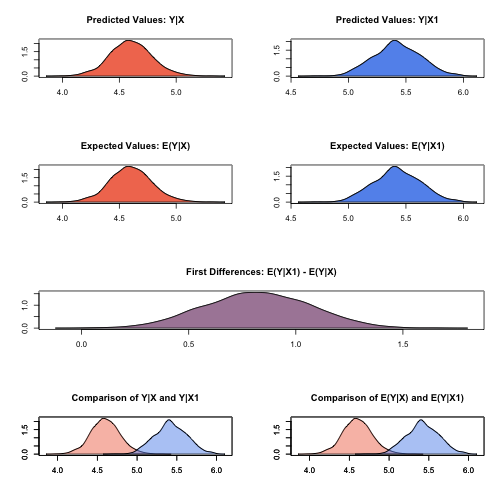
\includegraphics{Zelig-exp-1.png}
\caption{Zelig-exp}\end{figure}


\paragraph{Model}
\label{zelig-exp:model}
Let \(Y_i^*\) be the survival time for observation \(i\). This
variable might be censored for some observations at a fixed time
\(y_c\) such that the fully observed dependent variable,
\(Y_i\), is defined as
\begin{gather}
\begin{split}Y_i = \left\{ \begin{array}{ll}
      Y_i^* & \textrm{if }Y_i^* \leq y_c \\
      y_c & \textrm{if }Y_i^* > y_c \\
    \end{array} \right.\end{split}\notag
\end{gather}\begin{itemize}
\item {} 
The \emph{stochastic component} is described by the distribution of the
partially observed variable \(Y^*\). We assume \(Y_i^*\)
follows the exponential distribution whose density function is given
by
\begin{gather}
\begin{split}f(y_i^*\mid \lambda_i) = \frac{1}{\lambda_i} \exp\left(-\frac{y_i^*}{\lambda_i}\right)\end{split}\notag
\end{gather}
for \(y_i^*\ge 0\) and \(\lambda_i>0\). The mean of this
distribution is \(\lambda_i\).

In addition, survival models like the exponential have three
additional properties. The hazard function \(h(t)\) measures the
probability of not surviving past time \(t\) given survival up to
\(t\). In general, the hazard function is equal to
\(f(t)/S(t)\) where the survival function
\(S(t) = 1 - \int_{0}^t f(s) ds\) represents the fraction still
surviving at time \(t\). The cumulative hazard function
\(H(t)\) describes the probability of dying before time
\(t\). In general,
\(H(t)= \int_{0}^{t} h(s) ds = -\log S(t)\). In the case of the
exponential model,
\begin{gather}
\begin{split}\begin{aligned}
h(t) &=& \frac{1}{\lambda_i} \\
S(t) &=& \exp\left( -\frac{t}{\lambda_i} \right) \\
H(t) &=& \frac{t}{\lambda_i}\end{aligned}\end{split}\notag
\end{gather}
For the exponential model, the hazard function \(h(t)\) is
constant over time. The Weibull model and lognormal models allow the
hazard function to vary as a function of elapsed time (see and
respectively).

\item {} 
The \emph{systematic component} \(\lambda_i\) is modeled as
\begin{gather}
\begin{split}\lambda_i = \exp(x_i \beta),\end{split}\notag
\end{gather}
where \(x_i\) is the vector of explanatory variables, and
\(\beta\) is the vector of coefficients.

\end{itemize}


\paragraph{Quantities of Interest}
\label{zelig-exp:quantities-of-interest}\begin{itemize}
\item {} 
The expected values (qi\$ev) for the exponential model are simulations
of the expected duration given \(x_i\) and draws of \(\beta\)
from its posterior,
\begin{gather}
\begin{split}E(Y) = \lambda_i = \exp(x_i \beta).\end{split}\notag
\end{gather}
\item {} 
The predicted values (qi\$pr) are draws from the exponential
distribution with rate equal to the expected value.

\item {} 
The first difference (or difference in expected values, qi\$ev.diff),
is
\begin{gather}
\begin{split}\textrm{FD} \; = \; E(Y \mid x_1) - E(Y \mid x),\end{split}\notag
\end{gather}
where \(x\) and \(x_1\) are different vectors of values for
the explanatory variables.

\item {} 
In conditional prediction models, the average expected treatment
effect (att.ev) for the treatment group is
\begin{gather}
\begin{split}\frac{1}{\sum_{i=1}^n t_i}\sum_{i:t_i=1}^n \left\{ Y_i(t_i=1) - E[Y_i(t_i=0)]
  \right\},\end{split}\notag
\end{gather}
where \(t_i\) is a binary explanatory variable defining the
treatment (\(t_i=1\)) and control (\(t_i=0\)) groups. When
\(Y_i(t_i=1)\) is censored rather than observed, we replace it
with a simulation from the model given available knowledge of the
censoring process. Variation in the simulations is due to two
factors: uncertainty in the imputation process for censored
\(y_i^*\) and uncertainty in simulating \(E[Y_i(t_i=0)]\),
the counterfactual expected value of \(Y_i\) for observations in
the treatment group, under the assumption that everything stays the
same except that the treatment indicator is switched to
\(t_i=0\).

\item {} 
In conditional prediction models, the average predicted treatment
effect (att.pr) for the treatment group is
\begin{gather}
\begin{split}\frac{1}{\sum_{i=1}^n t_i}\sum_{i:t_i=1}^n \left\{ Y_i(t_i=1) -
  \widehat{Y_i(t_i=0)} \right\},\end{split}\notag
\end{gather}
where \(t_i\) is a binary explanatory variable defining the
treatment (\(t_i=1\)) and control (\(t_i=0\)) groups. When
\(Y_i(t_i=1)\) is censored rather than observed, we replace it
with a simulation from the model given available knowledge of the
censoring process. Variation in the simulations is due to two
factors: uncertainty in the imputation process for censored
\(y_i^*\) and uncertainty in simulating
\(\widehat{Y_i(t_i=0)}\), the counterfactual predicted value of
\(Y_i\) for observations in the treatment group, under the
assumption that everything stays the same except that the treatment
indicator is switched to \(t_i=0\).

\end{itemize}


\paragraph{Output Values}
\label{zelig-exp:output-values}
The output of each Zelig command contains useful information which you
may view. For example, if you run
\code{z.out \textless{}- zelig(Surv(Y, C) \textasciitilde{} X, model = exp, data)}, then you may
examine the available information in \code{z.out} by using
\code{names(z.out)}, see the coefficients by using z.out\$coefficients, and
a default summary of information through \code{summary(z.out)}.


\paragraph{See also}
\label{zelig-exp:see-also}
The exponential function is part of the survival library by Terry
Therneau, ported to R by Thomas Lumley. Advanced users may wish to refer
to \code{help(survfit)} in the survival library.


\subsubsection{zelig-gamma}
\label{zelig-gamma:zgamma}\label{zelig-gamma::doc}\label{zelig-gamma:zelig-gamma}
Gamma Regression for Continuous, Positive Dependent Variables

Use the gamma regression model if you have a positive-valued dependent
variable such as the number of years a parliamentary cabinet endures, or
the seconds you can stay airborne while jumping. The gamma distribution
assumes that all waiting times are complete by the end of the study
(censoring is not allowed).


\paragraph{Syntax}
\label{zelig-gamma:syntax}
With reference classes:

\begin{Verbatim}[commandchars=\\\{\}]
z5 \PYG{o}{\PYGZlt{}\PYGZhy{}} zgamma\PYG{o}{\PYGZdl{}}new\PYG{p}{(}\PYG{p}{)}
z5\PYG{o}{\PYGZdl{}}zelig\PYG{p}{(}Y \PYG{o}{\PYGZti{}} X1 \PYG{o}{+} X \PYG{o}{\PYGZti{}} X\PYG{p}{,} data \PYG{o}{=} mydata\PYG{p}{)}
z5\PYG{o}{\PYGZdl{}}setx\PYG{p}{(}\PYG{p}{)}
z5\PYG{o}{\PYGZdl{}}sim\PYG{p}{(}\PYG{p}{)}
\end{Verbatim}

With the Zelig 4 compatibility wrappers:

\begin{Verbatim}[commandchars=\\\{\}]
z.out \PYG{o}{\PYGZlt{}\PYGZhy{}} zelig\PYG{p}{(}Y \PYG{o}{\PYGZti{}} X1 \PYG{o}{+} X2\PYG{p}{,} model \PYG{o}{=} \PYG{l+s}{\PYGZdq{}}\PYG{l+s}{gamma\PYGZdq{}}\PYG{p}{,} data \PYG{o}{=} mydata\PYG{p}{)}
x.out \PYG{o}{\PYGZlt{}\PYGZhy{}} setx\PYG{p}{(}z.out\PYG{p}{)}
s.out \PYG{o}{\PYGZlt{}\PYGZhy{}} sim\PYG{p}{(}z.out\PYG{p}{,} x \PYG{o}{=} x.out\PYG{p}{,} x1 \PYG{o}{=} \PYG{k+kc}{NULL}\PYG{p}{)}
\end{Verbatim}


\paragraph{Example}
\label{zelig-gamma:example}
Attach the sample data:

\begin{Verbatim}[commandchars=\\\{\}]
data\PYG{p}{(}coalition\PYG{p}{)}
\end{Verbatim}

Estimate the model:

\begin{Verbatim}[commandchars=\\\{\}]
z.out \PYG{o}{\PYGZlt{}\PYGZhy{}} zelig\PYG{p}{(}duration \PYG{o}{\PYGZti{}} fract \PYG{o}{+} numst2\PYG{p}{,} model \PYG{o}{=} \PYG{l+s}{\PYGZdq{}}\PYG{l+s}{gamma\PYGZdq{}}\PYG{p}{,} data \PYG{o}{=} coalition\PYG{p}{)}
\end{Verbatim}

\begin{Verbatim}[commandchars=\\\{\}]
\PYG{c}{\PYGZsh{}\PYGZsh{} How to cite this model in Zelig:}
\PYG{c}{\PYGZsh{}\PYGZsh{}   Kosuke Imai, Gary King, Olivia Lau. 2007.}
\PYG{c}{\PYGZsh{}\PYGZsh{}   gamma: Gamma Regression for Continuous, Positive Dependent Variables}
\PYG{c}{\PYGZsh{}\PYGZsh{}   in Kosuke Imai, Gary King, and Olivia Lau, \PYGZdq{}Zelig: Everyone\PYGZsq{}s Statistical Software,\PYGZdq{}}
\PYG{c}{\PYGZsh{}\PYGZsh{}   http://zeligproject.org/}
\end{Verbatim}

View the regression output:

\begin{Verbatim}[commandchars=\\\{\}]
summary\PYG{p}{(}z.out\PYG{p}{)}
\end{Verbatim}

\begin{Verbatim}[commandchars=\\\{\}]
\PYG{c}{\PYGZsh{}\PYGZsh{} Model:}
\PYG{c}{\PYGZsh{}\PYGZsh{} \PYGZdl{}by}
\PYG{c}{\PYGZsh{}\PYGZsh{} [1] 1}
\PYG{c}{\PYGZsh{}\PYGZsh{}}
\PYG{c}{\PYGZsh{}\PYGZsh{}}
\PYG{c}{\PYGZsh{}\PYGZsh{} Call:  stats::glm(formula = duration \PYGZti{} fract + numst2, family = Gamma(\PYGZdq{}inverse\PYGZdq{}),}
\PYG{c}{\PYGZsh{}\PYGZsh{}     data = .)}
\PYG{c}{\PYGZsh{}\PYGZsh{}}
\PYG{c}{\PYGZsh{}\PYGZsh{} Coefficients:}
\PYG{c}{\PYGZsh{}\PYGZsh{} (Intercept)        fract       numst2}
\PYG{c}{\PYGZsh{}\PYGZsh{}  \PYGZhy{}0.0129597    0.0001149   \PYGZhy{}0.0173875}
\PYG{c}{\PYGZsh{}\PYGZsh{}}
\PYG{c}{\PYGZsh{}\PYGZsh{} Degrees of Freedom: 313 Total (i.e. Null);  311 Residual}
\PYG{c}{\PYGZsh{}\PYGZsh{} Null Deviance:       300.7}
\PYG{c}{\PYGZsh{}\PYGZsh{} Residual Deviance: 272.2         AIC: 2428}
\PYG{c}{\PYGZsh{}\PYGZsh{} Next step: Use \PYGZsq{}setx\PYGZsq{} method}
\end{Verbatim}

Set the baseline values (with the ruling coalition in the minority) and
the alternative values (with the ruling coalition in the majority) for
X:

\begin{Verbatim}[commandchars=\\\{\}]
x.low \PYG{o}{\PYGZlt{}\PYGZhy{}} setx\PYG{p}{(}z.out\PYG{p}{,} numst2 \PYG{o}{=} \PYG{l+m}{0}\PYG{p}{)}
x.high \PYG{o}{\PYGZlt{}\PYGZhy{}} setx\PYG{p}{(}z.out\PYG{p}{,} numst2 \PYG{o}{=} \PYG{l+m}{1}\PYG{p}{)}
\end{Verbatim}

Simulate expected values (qi\$ev) and first differences (qi\$fd):

\begin{Verbatim}[commandchars=\\\{\}]
s.out \PYG{o}{\PYGZlt{}\PYGZhy{}} sim\PYG{p}{(}z.out\PYG{p}{,} x \PYG{o}{=} x.low\PYG{p}{,} x1 \PYG{o}{=} x.high\PYG{p}{)}
\end{Verbatim}

\begin{Verbatim}[commandchars=\\\{\}]
summary\PYG{p}{(}s.out\PYG{p}{)}
\end{Verbatim}

\begin{Verbatim}[commandchars=\\\{\}]
\PYG{c}{\PYGZsh{}\PYGZsh{}}
\PYG{c}{\PYGZsh{}\PYGZsh{}  sim x :}
\PYG{c}{\PYGZsh{}\PYGZsh{}  \PYGZhy{}\PYGZhy{}\PYGZhy{}\PYGZhy{}\PYGZhy{}}
\PYG{c}{\PYGZsh{}\PYGZsh{} ev}
\PYG{c}{\PYGZsh{}\PYGZsh{}          mean       sd      50\PYGZpc{}     2.5\PYGZpc{}    97.5\PYGZpc{}}
\PYG{c}{\PYGZsh{}\PYGZsh{} [1,] 14.41947 1.064664 14.35618 12.51195 16.63425}
\PYG{c}{\PYGZsh{}\PYGZsh{} pv}
\PYG{c}{\PYGZsh{}\PYGZsh{}          mean       sd      50\PYGZpc{}      2.5\PYGZpc{}    97.5\PYGZpc{}}
\PYG{c}{\PYGZsh{}\PYGZsh{} [1,] 14.21243 12.60368 10.89322 0.6728363 47.30353}
\PYG{c}{\PYGZsh{}\PYGZsh{}}
\PYG{c}{\PYGZsh{}\PYGZsh{}  sim x1 :}
\PYG{c}{\PYGZsh{}\PYGZsh{}  \PYGZhy{}\PYGZhy{}\PYGZhy{}\PYGZhy{}\PYGZhy{}}
\PYG{c}{\PYGZsh{}\PYGZsh{} ev}
\PYG{c}{\PYGZsh{}\PYGZsh{}          mean       sd      50\PYGZpc{}    2.5\PYGZpc{}    97.5\PYGZpc{}}
\PYG{c}{\PYGZsh{}\PYGZsh{} [1,] 19.19869 1.133553 19.11127 17.1843 21.62197}
\PYG{c}{\PYGZsh{}\PYGZsh{} pv}
\PYG{c}{\PYGZsh{}\PYGZsh{}          mean       sd      50\PYGZpc{}      2.5\PYGZpc{}    97.5\PYGZpc{}}
\PYG{c}{\PYGZsh{}\PYGZsh{} [1,] 18.60736 16.66119 13.88459 0.9246994 61.53045}
\PYG{c}{\PYGZsh{}\PYGZsh{} fd}
\PYG{c}{\PYGZsh{}\PYGZsh{}          mean       sd      50\PYGZpc{}     2.5\PYGZpc{}    97.5\PYGZpc{}}
\PYG{c}{\PYGZsh{}\PYGZsh{} [1,] 4.779217 1.535785 4.734045 1.825047 7.751185}
\end{Verbatim}

\begin{Verbatim}[commandchars=\\\{\}]
plot\PYG{p}{(}s.out\PYG{p}{)}
\end{Verbatim}
\begin{figure}[htbp]
\centering
\capstart

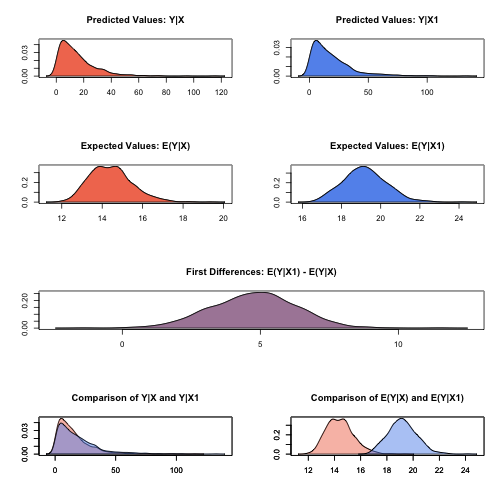
\includegraphics{Zelig-gamma-1.png}
\caption{Zelig-gamma}\end{figure}


\paragraph{Model}
\label{zelig-gamma:model}\begin{itemize}
\item {} 
The Gamma distribution with scale parameter \(\alpha\) has a
\emph{stochastic component}:
\begin{gather}
\begin{split}\begin{aligned}
Y &\sim& \textrm{Gamma}(y_i \mid \lambda_i, \alpha) \\
f(y)  &=& \frac{1}{\alpha^{\lambda_i} \, \Gamma \lambda_i} \, y_i^{\lambda_i
  - 1} \exp -\left\{ \frac{y_i}{\alpha} \right\}\end{aligned}\end{split}\notag
\end{gather}
\begin{DUlineblock}{0em}
\item[] for \(\alpha, \lambda_i, y_i > 0\).
\end{DUlineblock}

\item {} 
The \emph{systematic component} is given by
\begin{gather}
\begin{split}\lambda_i = \frac{1}{x_i \beta}\end{split}\notag
\end{gather}
\end{itemize}


\paragraph{Quantities of Interest}
\label{zelig-gamma:quantities-of-interest}\begin{itemize}
\item {} 
The expected values (qi\$ev) are simulations of the mean of the
stochastic component given draws of \(\alpha\) and \(\beta\)
from their posteriors:
\begin{gather}
\begin{split}E(Y) = \alpha \lambda_i.\end{split}\notag
\end{gather}
\item {} 
The predicted values (qi\$pr) are draws from the gamma distribution
for each given set of parameters \((\alpha, \lambda_i)\).

\item {} 
If x1 is specified, sim() also returns the differences in the
expected values (qi\$fd),
\begin{gather}
\begin{split}E(Y \mid x_1) -
  E(Y \mid x)\end{split}\notag
\end{gather}
.

\item {} 
In conditional prediction models, the average expected treatment
effect (att.ev) for the treatment group is
\begin{gather}
\begin{split}\frac{1}{\sum_{i=1}^n t_i}\sum_{i:t_i=1}^n \left\{ Y_i(t_i=1) -
      E[Y_i(t_i=0)] \right\},\end{split}\notag
\end{gather}
where \(t_i\) is a binary explanatory variable defining the
treatment (\(t_i=1\)) and control (\(t_i=0\)) groups.
Variation in the simulations are due to uncertainty in simulating
\(E[Y_i(t_i=0)]\), the counterfactual expected value of
\(Y_i\) for observations in the treatment group, under the
assumption that everything stays the same except that the treatment
indicator is switched to \(t_i=0\).

\item {} 
In conditional prediction models, the average predicted treatment
effect (att.pr) for the treatment group is
\begin{gather}
\begin{split}\frac{1}{\sum_{i=1}^n t_i}\sum_{i:t_i=1}^n \left\{ Y_i(t_i=1) -
      \widehat{Y_i(t_i=0)} \right\},\end{split}\notag
\end{gather}
where \(t_i\) is a binary explanatory variable defining the
treatment (\(t_i=1\)) and control (\(t_i=0\)) groups.
Variation in the simulations are due to uncertainty in simulating
\(\widehat{Y_i(t_i=0)}\), the counterfactual predicted value of
\(Y_i\) for observations in the treatment group, under the
assumption that everything stays the same except that the treatment
indicator is switched to \(t_i=0\).

\end{itemize}


\paragraph{Output Values}
\label{zelig-gamma:output-values}
The output of each Zelig command contains useful information which you
may view. For example, if you run
\code{z.out \textless{}- zelig(y \textasciitilde{} x, model = gamma, data)}, then you may examine the
available information in \code{z.out} by using \code{names(z.out)}, see the
coefficients by using z.out\$coefficients, and a default summary of
information through \code{summary(z.out)}.


\paragraph{See also}
\label{zelig-gamma:see-also}
The gamma model is part of the stats package. Advanced users may
wish to refer to \code{help(glm)} and \code{help(family)}.


\subsubsection{zelig-logit}
\label{zelig-logit:zelig-logit}\label{zelig-logit::doc}\label{zelig-logit:zlogit}
Logistic Regression for Dichotomous Dependent Variables

Logistic regression specifies a dichotomous dependent variable as a
function of a set of explanatory variables.


\paragraph{Syntax}
\label{zelig-logit:syntax}
With reference classes:

\begin{Verbatim}[commandchars=\\\{\}]
z5 \PYG{o}{\PYGZlt{}\PYGZhy{}} zlogit\PYG{o}{\PYGZdl{}}new\PYG{p}{(}\PYG{p}{)}
z5\PYG{o}{\PYGZdl{}}zelig\PYG{p}{(}Y \PYG{o}{\PYGZti{}} X1 \PYG{o}{+} X \PYG{o}{\PYGZti{}} X\PYG{p}{,} data \PYG{o}{=} mydata\PYG{p}{)}
z5\PYG{o}{\PYGZdl{}}setx\PYG{p}{(}\PYG{p}{)}
z5\PYG{o}{\PYGZdl{}}sim\PYG{p}{(}\PYG{p}{)}
\end{Verbatim}

With the Zelig 4 compatibility wrappers:

\begin{Verbatim}[commandchars=\\\{\}]
z.out \PYG{o}{\PYGZlt{}\PYGZhy{}} zelig\PYG{p}{(}Y \PYG{o}{\PYGZti{}} X1 \PYG{o}{+} X2\PYG{p}{,} model \PYG{o}{=} \PYG{l+s}{\PYGZdq{}}\PYG{l+s}{logit\PYGZdq{}}\PYG{p}{,} data \PYG{o}{=} mydata\PYG{p}{)}
x.out \PYG{o}{\PYGZlt{}\PYGZhy{}} setx\PYG{p}{(}z.out\PYG{p}{)}
s.out \PYG{o}{\PYGZlt{}\PYGZhy{}} sim\PYG{p}{(}z.out\PYG{p}{,} x \PYG{o}{=} x.out\PYG{p}{,} x1 \PYG{o}{=} \PYG{k+kc}{NULL}\PYG{p}{)}
\end{Verbatim}


\paragraph{Examples}
\label{zelig-logit:examples}

\subparagraph{Basic Example}
\label{zelig-logit:basic-example}
Attaching the sample turnout dataset:

\begin{Verbatim}[commandchars=\\\{\}]
data\PYG{p}{(}turnout\PYG{p}{)}
\end{Verbatim}

Estimating parameter values for the logistic regression:

\begin{Verbatim}[commandchars=\\\{\}]
z.out1 \PYG{o}{\PYGZlt{}\PYGZhy{}} zelig\PYG{p}{(}vote \PYG{o}{\PYGZti{}} age \PYG{o}{+} race\PYG{p}{,} model \PYG{o}{=} \PYG{l+s}{\PYGZdq{}}\PYG{l+s}{logit\PYGZdq{}}\PYG{p}{,} data \PYG{o}{=} turnout\PYG{p}{)}
\end{Verbatim}

\begin{Verbatim}[commandchars=\\\{\}]
\PYG{c}{\PYGZsh{}\PYGZsh{} How to cite this model in Zelig:}
\PYG{c}{\PYGZsh{}\PYGZsh{}   Kosuke Imai, Gary King, Olivia Lau. 2007.}
\PYG{c}{\PYGZsh{}\PYGZsh{}   logit: Logistic Regression for Dichotomous Dependent Variables}
\PYG{c}{\PYGZsh{}\PYGZsh{}   in Kosuke Imai, Gary King, and Olivia Lau, \PYGZdq{}Zelig: Everyone\PYGZsq{}s Statistical Software,\PYGZdq{}}
\PYG{c}{\PYGZsh{}\PYGZsh{}   http://zeligproject.org/}
\end{Verbatim}

Setting values for the explanatory variables:

\begin{Verbatim}[commandchars=\\\{\}]
x.out1 \PYG{o}{\PYGZlt{}\PYGZhy{}} setx\PYG{p}{(}z.out1\PYG{p}{,} age \PYG{o}{=} \PYG{l+m}{36}\PYG{p}{,} race \PYG{o}{=} \PYG{l+s}{\PYGZdq{}}\PYG{l+s}{white\PYGZdq{}}\PYG{p}{)}
\end{Verbatim}

Simulating quantities of interest from the posterior distribution.

\begin{Verbatim}[commandchars=\\\{\}]
s.out1 \PYG{o}{\PYGZlt{}\PYGZhy{}} sim\PYG{p}{(}z.out1\PYG{p}{,} x \PYG{o}{=} x.out1\PYG{p}{)}
\end{Verbatim}

\begin{Verbatim}[commandchars=\\\{\}]
summary\PYG{p}{(}s.out1\PYG{p}{)}
\end{Verbatim}

\begin{Verbatim}[commandchars=\\\{\}]
\PYG{c}{\PYGZsh{}\PYGZsh{}}
\PYG{c}{\PYGZsh{}\PYGZsh{}  sim x :}
\PYG{c}{\PYGZsh{}\PYGZsh{}  \PYGZhy{}\PYGZhy{}\PYGZhy{}\PYGZhy{}\PYGZhy{}}
\PYG{c}{\PYGZsh{}\PYGZsh{} ev}
\PYG{c}{\PYGZsh{}\PYGZsh{}           mean         sd      50\PYGZpc{}     2.5\PYGZpc{}     97.5\PYGZpc{}}
\PYG{c}{\PYGZsh{}\PYGZsh{} [1,] 0.7479394 0.01193434 0.748012 0.724231 0.7712138}
\PYG{c}{\PYGZsh{}\PYGZsh{} pv}
\PYG{c}{\PYGZsh{}\PYGZsh{}          0     1}
\PYG{c}{\PYGZsh{}\PYGZsh{} [1,] 0.278 0.722}
\end{Verbatim}

\begin{Verbatim}[commandchars=\\\{\}]
plot\PYG{p}{(}s.out1\PYG{p}{)}
\end{Verbatim}
\begin{figure}[htbp]
\centering
\capstart


\includegraphics{Zelig-logit-1-1.png}
\caption{Zelig-logit-1}\end{figure}


\subparagraph{Simulating First Differences}
\label{zelig-logit:simulating-first-differences}
Estimating the risk difference (and risk ratio) between low education
(25th percentile) and high education (75th percentile) while all the
other variables held at their default values.

\begin{Verbatim}[commandchars=\\\{\}]
z.out2 \PYG{o}{\PYGZlt{}\PYGZhy{}} zelig\PYG{p}{(}vote \PYG{o}{\PYGZti{}} race \PYG{o}{+} educate\PYG{p}{,} model \PYG{o}{=} \PYG{l+s}{\PYGZdq{}}\PYG{l+s}{logit\PYGZdq{}}\PYG{p}{,} data \PYG{o}{=} turnout\PYG{p}{)}
\end{Verbatim}

\begin{Verbatim}[commandchars=\\\{\}]
\PYG{c}{\PYGZsh{}\PYGZsh{} How to cite this model in Zelig:}
\PYG{c}{\PYGZsh{}\PYGZsh{}   Kosuke Imai, Gary King, Olivia Lau. 2007.}
\PYG{c}{\PYGZsh{}\PYGZsh{}   logit: Logistic Regression for Dichotomous Dependent Variables}
\PYG{c}{\PYGZsh{}\PYGZsh{}   in Kosuke Imai, Gary King, and Olivia Lau, \PYGZdq{}Zelig: Everyone\PYGZsq{}s Statistical Software,\PYGZdq{}}
\PYG{c}{\PYGZsh{}\PYGZsh{}   http://zeligproject.org/}
\end{Verbatim}

\begin{Verbatim}[commandchars=\\\{\}]
x.high \PYG{o}{\PYGZlt{}\PYGZhy{}} setx\PYG{p}{(}z.out2\PYG{p}{,} educate \PYG{o}{=} quantile\PYG{p}{(}turnout\PYG{o}{\PYGZdl{}}educate\PYG{p}{,} prob \PYG{o}{=} \PYG{l+m}{0.75}\PYG{p}{)}\PYG{p}{)}
x.low \PYG{o}{\PYGZlt{}\PYGZhy{}} setx\PYG{p}{(}z.out2\PYG{p}{,} educate \PYG{o}{=} quantile\PYG{p}{(}turnout\PYG{o}{\PYGZdl{}}educate\PYG{p}{,} prob \PYG{o}{=} \PYG{l+m}{0.25}\PYG{p}{)}\PYG{p}{)}
s.out2 \PYG{o}{\PYGZlt{}\PYGZhy{}} sim\PYG{p}{(}z.out2\PYG{p}{,} x \PYG{o}{=} x.high\PYG{p}{,} x1 \PYG{o}{=} x.low\PYG{p}{)}
summary\PYG{p}{(}s.out2\PYG{p}{)}
\end{Verbatim}

\begin{Verbatim}[commandchars=\\\{\}]
\PYG{c}{\PYGZsh{}\PYGZsh{}}
\PYG{c}{\PYGZsh{}\PYGZsh{}  sim x :}
\PYG{c}{\PYGZsh{}\PYGZsh{}  \PYGZhy{}\PYGZhy{}\PYGZhy{}\PYGZhy{}\PYGZhy{}}
\PYG{c}{\PYGZsh{}\PYGZsh{} ev}
\PYG{c}{\PYGZsh{}\PYGZsh{}           mean         sd       50\PYGZpc{}      2.5\PYGZpc{}     97.5\PYGZpc{}}
\PYG{c}{\PYGZsh{}\PYGZsh{} [1,] 0.8221088 0.01046643 0.8225926 0.7989981 0.8425136}
\PYG{c}{\PYGZsh{}\PYGZsh{} pv}
\PYG{c}{\PYGZsh{}\PYGZsh{}          0     1}
\PYG{c}{\PYGZsh{}\PYGZsh{} [1,] 0.172 0.828}
\PYG{c}{\PYGZsh{}\PYGZsh{}}
\PYG{c}{\PYGZsh{}\PYGZsh{}  sim x1 :}
\PYG{c}{\PYGZsh{}\PYGZsh{}  \PYGZhy{}\PYGZhy{}\PYGZhy{}\PYGZhy{}\PYGZhy{}}
\PYG{c}{\PYGZsh{}\PYGZsh{} ev}
\PYG{c}{\PYGZsh{}\PYGZsh{}           mean         sd      50\PYGZpc{}      2.5\PYGZpc{}    97.5\PYGZpc{}}
\PYG{c}{\PYGZsh{}\PYGZsh{} [1,] 0.7091027 0.01317142 0.708915 0.6826494 0.734145}
\PYG{c}{\PYGZsh{}\PYGZsh{} pv}
\PYG{c}{\PYGZsh{}\PYGZsh{}          0     1}
\PYG{c}{\PYGZsh{}\PYGZsh{} [1,] 0.303 0.697}
\PYG{c}{\PYGZsh{}\PYGZsh{} fd}
\PYG{c}{\PYGZsh{}\PYGZsh{}            mean        sd        50\PYGZpc{}       2.5\PYGZpc{}       97.5\PYGZpc{}}
\PYG{c}{\PYGZsh{}\PYGZsh{} [1,] \PYGZhy{}0.1130061 0.0116836 \PYGZhy{}0.1131443 \PYGZhy{}0.1363372 \PYGZhy{}0.09073965}
\end{Verbatim}

\begin{Verbatim}[commandchars=\\\{\}]
plot\PYG{p}{(}s.out2\PYG{p}{)}
\end{Verbatim}
\begin{figure}[htbp]
\centering
\capstart

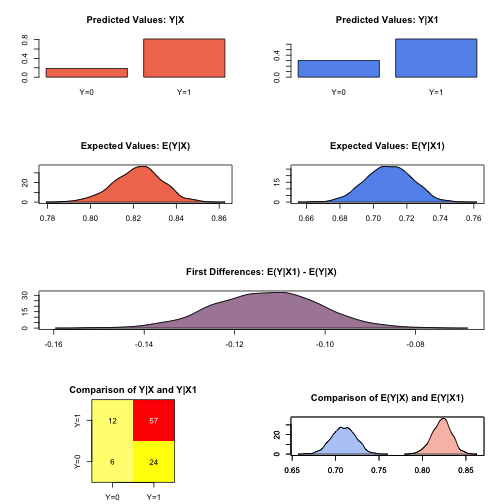
\includegraphics{Zelig-logit-2-1.png}
\caption{Zelig-logit-2}\end{figure}


\paragraph{Model}
\label{zelig-logit:model}
Let \(Y_i\) be the binary dependent variable for observation
\(i\) which takes the value of either 0 or 1.
\begin{itemize}
\item {} 
The \emph{stochastic component} is given by
\begin{gather}
\begin{split}\begin{aligned}
Y_i &\sim& \textrm{Bernoulli}(y_i \mid \pi_i) \\
    &=& \pi_i^{y_i} (1-\pi_i)^{1-y_i}\end{aligned}\end{split}\notag
\end{gather}
where \(\pi_i=\Pr(Y_i=1)\).

\item {} 
The \emph{systematic component} is given by:
\begin{gather}
\begin{split}\pi_i \; = \; \frac{1}{1 + \exp(-x_i \beta)}.\end{split}\notag
\end{gather}
where \(x_i\) is the vector of \(k\) explanatory variables
for observation \(i\) and \(\beta\) is the vector of
coefficients.

\end{itemize}


\paragraph{Quantities of Interest}
\label{zelig-logit:quantities-of-interest}\begin{itemize}
\item {} 
The expected values (qi\$ev) for the logit model are simulations of
the predicted probability of a success:
\begin{gather}
\begin{split}E(Y) =
  \pi_i= \frac{1}{1 + \exp(-x_i \beta)},\end{split}\notag
\end{gather}
given draws of \(\beta\) from its sampling distribution.

\item {} 
The predicted values (qi\$pr) are draws from the Binomial distribution
with mean equal to the simulated expected value \(\pi_i\).

\item {} 
The first difference (qi\$fd) for the logit model is defined as
\begin{gather}
\begin{split}\textrm{FD} = \Pr(Y = 1 \mid x_1) - \Pr(Y = 1 \mid x).\end{split}\notag
\end{gather}
\item {} 
The risk ratio (qi\$rr) is defined as
\begin{gather}
\begin{split}\textrm{RR} = \Pr(Y = 1 \mid x_1) \ / \ \Pr(Y = 1 \mid x).\end{split}\notag
\end{gather}
\item {} 
In conditional prediction models, the average expected treatment
effect (att.ev) for the treatment group is
\begin{gather}
\begin{split}\frac{1}{\sum_{i=1}^n t_i}\sum_{i:t_i=1}^n \left\{ Y_i(t_i=1) -
      E[Y_i(t_i=0)] \right\},\end{split}\notag
\end{gather}
where \(t_i\) is a binary explanatory variable defining the
treatment (\(t_i=1\)) and control (\(t_i=0\)) groups.
Variation in the simulations are due to uncertainty in simulating
\(E[Y_i(t_i=0)]\), the counterfactual expected value of
\(Y_i\) for observations in the treatment group, under the
assumption that everything stays the same except that the treatment
indicator is switched to \(t_i=0\).

\item {} 
In conditional prediction models, the average predicted treatment
effect (att.pr) for the treatment group is
\begin{gather}
\begin{split}\frac{1}{\sum_{i=1}^n t_i}\sum_{i:t_i=1}^n \left\{ Y_i(t_i=1) -
      \widehat{Y_i(t_i=0)}\right\},\end{split}\notag
\end{gather}
where \(t_i\) is a binary explanatory variable defining the
treatment (\(t_i=1\)) and control (\(t_i=0\)) groups.
Variation in the simulations are due to uncertainty in simulating
\(\widehat{Y_i(t_i=0)}\), the counterfactual predicted value of
\(Y_i\) for observations in the treatment group, under the
assumption that everything stays the same except that the treatment
indicator is switched to \(t_i=0\).

\end{itemize}


\paragraph{Output Values}
\label{zelig-logit:output-values}
The output of each Zelig command contains useful information which you
may view. For example, if you run
\code{z.out \textless{}- zelig(y \textasciitilde{} x, model = logit, data)}, then you may examine the
available information in \code{z.out} by using \code{names(z.out)}, see the
coefficients by using z.out\$coefficients, and a default summary of
information through \code{summary(z.out)}.


\paragraph{See also}
\label{zelig-logit:see-also}
The logit model is part of the stats package. Advanced users may
wish to refer to \code{help(glm)} and \code{help(family)}.


\subsubsection{zelig-lognorm}
\label{zelig-lognorm:zelig-lognorm}\label{zelig-lognorm::doc}\label{zelig-lognorm:zlognorm}
Log-Normal Regression for Duration Dependent Variables

The log-normal model describes an event’s duration, the dependent
variable, as a function of a set of explanatory variables. The
log-normal model may take time censored dependent variables, and allows
the hazard rate to increase and decrease.


\paragraph{Syntax}
\label{zelig-lognorm:syntax}
With reference classes:

\begin{Verbatim}[commandchars=\\\{\}]
z5 \PYG{o}{\PYGZlt{}\PYGZhy{}} zlognorm\PYG{o}{\PYGZdl{}}new\PYG{p}{(}\PYG{p}{)}
z5\PYG{o}{\PYGZdl{}}zelig\PYG{p}{(}Surv\PYG{p}{(}Y\PYG{p}{,} C\PYG{p}{)} \PYG{o}{\PYGZti{}} X\PYG{p}{,} data \PYG{o}{=} mydata\PYG{p}{)}
z5\PYG{o}{\PYGZdl{}}setx\PYG{p}{(}\PYG{p}{)}
z5\PYG{o}{\PYGZdl{}}sim\PYG{p}{(}\PYG{p}{)}
\end{Verbatim}

With reference classes:

\begin{Verbatim}[commandchars=\\\{\}]
z5 \PYG{o}{\PYGZlt{}\PYGZhy{}} zlognorm\PYG{o}{\PYGZdl{}}new\PYG{p}{(}\PYG{p}{)}
z5\PYG{o}{\PYGZdl{}}zelig\PYG{p}{(}Surv\PYG{p}{(}Y\PYG{p}{,} C\PYG{p}{)} \PYG{o}{\PYGZti{}} X\PYG{p}{,} data \PYG{o}{=} mydata\PYG{p}{)}
z5\PYG{o}{\PYGZdl{}}setx\PYG{p}{(}\PYG{p}{)}
z5\PYG{o}{\PYGZdl{}}sim\PYG{p}{(}\PYG{p}{)}
\end{Verbatim}

With the Zelig 4 compatibility wrappers:

\begin{Verbatim}[commandchars=\\\{\}]
z.out \PYG{o}{\PYGZlt{}\PYGZhy{}} zelig\PYG{p}{(}Surv\PYG{p}{(}Y\PYG{p}{,} C\PYG{p}{)} \PYG{o}{\PYGZti{}} X\PYG{p}{,} model \PYG{o}{=} \PYG{l+s}{\PYGZdq{}}\PYG{l+s}{lognorm\PYGZdq{}}\PYG{p}{,} data \PYG{o}{=} mydata\PYG{p}{)}
x.out \PYG{o}{\PYGZlt{}\PYGZhy{}} setx\PYG{p}{(}z.out\PYG{p}{)}
s.out \PYG{o}{\PYGZlt{}\PYGZhy{}} sim\PYG{p}{(}z.out\PYG{p}{,} x \PYG{o}{=} x.out\PYG{p}{)}
\end{Verbatim}

Log-normal models require that the dependent variable be in the form
Surv(Y, C), where Y and C are vectors of length \(n\). For each
observation \(i\) in 1, …, \(n\), the value \(y_i\) is the
duration (lifetime, for example) of each subject, and the associated
\(c_i\) is a binary variable such that \(c_i = 1\) if the
duration is not censored (\emph{e.g.}, the subject dies during the study) or
\(c_i = 0\) if the duration is censored (\emph{e.g.}, the subject is
still alive at the end of the study). If \(c_i\) is omitted, all Y
are assumed to be completed; that is, time defaults to 1 for all
observations.


\paragraph{Input Values}
\label{zelig-lognorm:input-values}
In addition to the standard inputs, zelig() takes the following
additional options for lognormal regression:
\begin{itemize}
\item {} 
robust: defaults to FALSE. If TRUE, zelig() computes robust standard
errors based on sandwich estimators (see and ) based on the options
in cluster.

\item {} 
cluster: if robust = TRUE, you may select a variable to define groups
of correlated observations. Let x3 be a variable that consists of
either discrete numeric values, character strings, or factors that
define strata. Then

\end{itemize}

\begin{Verbatim}[commandchars=\\\{\}]
z.out \PYG{o}{\PYGZlt{}\PYGZhy{}} zelig\PYG{p}{(}y \PYG{o}{\PYGZti{}} x1 \PYG{o}{+} x2\PYG{p}{,} robust \PYG{o}{=} \PYG{k+kc}{TRUE}\PYG{p}{,} cluster \PYG{o}{=} \PYG{l+s}{\PYGZdq{}}\PYG{l+s}{x3\PYGZdq{}}\PYG{p}{,} model \PYG{o}{=} \PYG{l+s}{\PYGZdq{}}\PYG{l+s}{exp\PYGZdq{}}\PYG{p}{,} data \PYG{o}{=} mydata\PYG{p}{)}
\end{Verbatim}

means that the observations can be correlated within the strata
defined by the variable x3, and that robust standard errors should be
calculated according to those clusters. If robust = TRUE but cluster
is not specified, zelig() assumes that each observation falls into
its own cluster.


\paragraph{Example}
\label{zelig-lognorm:example}
Attach the sample data:

\begin{Verbatim}[commandchars=\\\{\}]
data\PYG{p}{(}coalition\PYG{p}{)}
\end{Verbatim}

Estimate the model:

\begin{Verbatim}[commandchars=\\\{\}]
z.out \PYG{o}{\PYGZlt{}\PYGZhy{}} zelig\PYG{p}{(}Surv\PYG{p}{(}duration\PYG{p}{,} ciep12\PYG{p}{)} \PYG{o}{\PYGZti{}} fract \PYG{o}{+} numst2\PYG{p}{,} model \PYG{o}{=}\PYG{l+s}{\PYGZdq{}}\PYG{l+s}{lognorm\PYGZdq{}}\PYG{p}{,}  data \PYG{o}{=} coalition\PYG{p}{)}
\end{Verbatim}

\begin{Verbatim}[commandchars=\\\{\}]
\PYG{c}{\PYGZsh{}\PYGZsh{} How to cite this model in Zelig:}
\PYG{c}{\PYGZsh{}\PYGZsh{}   Matthew Owen, Olivia Lau, Kosuke Imai, Gary King. 2007.}
\PYG{c}{\PYGZsh{}\PYGZsh{}   lognorm: Log\PYGZhy{}Normal Regression for Duration Dependent Variables}
\PYG{c}{\PYGZsh{}\PYGZsh{}   in Kosuke Imai, Gary King, and Olivia Lau, \PYGZdq{}Zelig: Everyone\PYGZsq{}s Statistical Software,\PYGZdq{}}
\PYG{c}{\PYGZsh{}\PYGZsh{}   http://zeligproject.org/}
\end{Verbatim}

View the regression output:

\begin{Verbatim}[commandchars=\\\{\}]
summary\PYG{p}{(}z.out\PYG{p}{)}
\end{Verbatim}

\begin{Verbatim}[commandchars=\\\{\}]
\PYG{c}{\PYGZsh{}\PYGZsh{} Model:}
\PYG{c}{\PYGZsh{}\PYGZsh{} \PYGZdl{}by}
\PYG{c}{\PYGZsh{}\PYGZsh{} [1] 1}
\PYG{c}{\PYGZsh{}\PYGZsh{}}
\PYG{c}{\PYGZsh{}\PYGZsh{} Call:}
\PYG{c}{\PYGZsh{}\PYGZsh{} survival::survreg(formula = Surv(duration, ciep12) \PYGZti{} fract +}
\PYG{c}{\PYGZsh{}\PYGZsh{}     numst2, data = ., dist = \PYGZdq{}lognormal\PYGZdq{}, model = FALSE)}
\PYG{c}{\PYGZsh{}\PYGZsh{}}
\PYG{c}{\PYGZsh{}\PYGZsh{} Coefficients:}
\PYG{c}{\PYGZsh{}\PYGZsh{} (Intercept)       fract      numst2}
\PYG{c}{\PYGZsh{}\PYGZsh{}  5.36666977 \PYGZhy{}0.00443755  0.55983251}
\PYG{c}{\PYGZsh{}\PYGZsh{}}
\PYG{c}{\PYGZsh{}\PYGZsh{} Scale= 1.20008}
\PYG{c}{\PYGZsh{}\PYGZsh{}}
\PYG{c}{\PYGZsh{}\PYGZsh{} Loglik(model)= \PYGZhy{}1077.9   Loglik(intercept only)= \PYGZhy{}1101.2}
\PYG{c}{\PYGZsh{}\PYGZsh{}  Chisq= 46.58 on 2 degrees of freedom, p= 7.7e\PYGZhy{}11}
\PYG{c}{\PYGZsh{}\PYGZsh{} n= 314}
\PYG{c}{\PYGZsh{}\PYGZsh{} Next step: Use \PYGZsq{}setx\PYGZsq{} method}
\end{Verbatim}

Set the baseline values (with the ruling coalition in the minority) and
the alternative values (with the ruling coalition in the majority) for
X:

\begin{Verbatim}[commandchars=\\\{\}]
x.low \PYG{o}{\PYGZlt{}\PYGZhy{}} setx\PYG{p}{(}z.out\PYG{p}{,} numst2 \PYG{o}{=} \PYG{l+m}{0}\PYG{p}{)}
\end{Verbatim}

\begin{Verbatim}[commandchars=\\\{\}]
\PYG{c}{\PYGZsh{}\PYGZsh{} Error in terms(lm(formula, data), \PYGZdq{}predvars\PYGZdq{}): error in evaluating the argument \PYGZsq{}x\PYGZsq{} in selecting a method for function \PYGZsq{}terms\PYGZsq{}: Error in Ops.Surv(y, z\PYGZdl{}residuals) : Invalid operation on a survival time}
\PYG{c}{\PYGZsh{}\PYGZsh{} Calls: lm \PYGZhy{}\PYGZgt{} lm.fit \PYGZhy{}\PYGZgt{} Ops.Surv}
\end{Verbatim}

\begin{Verbatim}[commandchars=\\\{\}]
x.high \PYG{o}{\PYGZlt{}\PYGZhy{}} setx\PYG{p}{(}z.out\PYG{p}{,} numst2\PYG{o}{=} \PYG{l+m}{1}\PYG{p}{)}
\end{Verbatim}

\begin{Verbatim}[commandchars=\\\{\}]
\PYG{c}{\PYGZsh{}\PYGZsh{} Error in terms(lm(formula, data), \PYGZdq{}predvars\PYGZdq{}): error in evaluating the argument \PYGZsq{}x\PYGZsq{} in selecting a method for function \PYGZsq{}terms\PYGZsq{}: Error in Ops.Surv(y, z\PYGZdl{}residuals) : Invalid operation on a survival time}
\PYG{c}{\PYGZsh{}\PYGZsh{} Calls: lm \PYGZhy{}\PYGZgt{} lm.fit \PYGZhy{}\PYGZgt{} Ops.Surv}
\end{Verbatim}

Simulate expected values (qi\$ev) and first differences (qi\$fd):

\begin{Verbatim}[commandchars=\\\{\}]
s.out \PYG{o}{\PYGZlt{}\PYGZhy{}} sim\PYG{p}{(}z.out\PYG{p}{,} x \PYG{o}{=} x.low\PYG{p}{,} x1 \PYG{o}{=} x.high\PYG{p}{)}
\end{Verbatim}

\begin{Verbatim}[commandchars=\\\{\}]
summary\PYG{p}{(}s.out\PYG{p}{)}
\end{Verbatim}

\begin{Verbatim}[commandchars=\\\{\}]
\PYG{c}{\PYGZsh{}\PYGZsh{}}
\PYG{c}{\PYGZsh{}\PYGZsh{}  sim x :}
\PYG{c}{\PYGZsh{}\PYGZsh{}  \PYGZhy{}\PYGZhy{}\PYGZhy{}\PYGZhy{}\PYGZhy{}}
\PYG{c}{\PYGZsh{}\PYGZsh{} ev}
\PYG{c}{\PYGZsh{}\PYGZsh{}           mean         sd      50\PYGZpc{}      2.5\PYGZpc{}     97.5\PYGZpc{}}
\PYG{c}{\PYGZsh{}\PYGZsh{} [1,] 0.7098857 0.01311726 0.709487 0.6856631 0.7358735}
\PYG{c}{\PYGZsh{}\PYGZsh{} pv}
\PYG{c}{\PYGZsh{}\PYGZsh{}          0     1}
\PYG{c}{\PYGZsh{}\PYGZsh{} [1,] 0.298 0.702}
\PYG{c}{\PYGZsh{}\PYGZsh{}}
\PYG{c}{\PYGZsh{}\PYGZsh{}  sim x1 :}
\PYG{c}{\PYGZsh{}\PYGZsh{}  \PYGZhy{}\PYGZhy{}\PYGZhy{}\PYGZhy{}\PYGZhy{}}
\PYG{c}{\PYGZsh{}\PYGZsh{} ev}
\PYG{c}{\PYGZsh{}\PYGZsh{}           mean        sd       50\PYGZpc{}      2.5\PYGZpc{}     97.5\PYGZpc{}}
\PYG{c}{\PYGZsh{}\PYGZsh{} [1,] 0.8230556 0.0105009 0.8227265 0.8028129 0.8433327}
\PYG{c}{\PYGZsh{}\PYGZsh{} pv}
\PYG{c}{\PYGZsh{}\PYGZsh{}         0    1}
\PYG{c}{\PYGZsh{}\PYGZsh{} [1,] 0.18 0.82}
\PYG{c}{\PYGZsh{}\PYGZsh{} fd}
\PYG{c}{\PYGZsh{}\PYGZsh{}           mean         sd       50\PYGZpc{}       2.5\PYGZpc{}     97.5\PYGZpc{}}
\PYG{c}{\PYGZsh{}\PYGZsh{} [1,] 0.1131699 0.01186652 0.1134081 0.09045198 0.1366067}
\end{Verbatim}

\begin{Verbatim}[commandchars=\\\{\}]
plot\PYG{p}{(}s.out\PYG{p}{)}
\end{Verbatim}
\begin{figure}[htbp]
\centering
\capstart

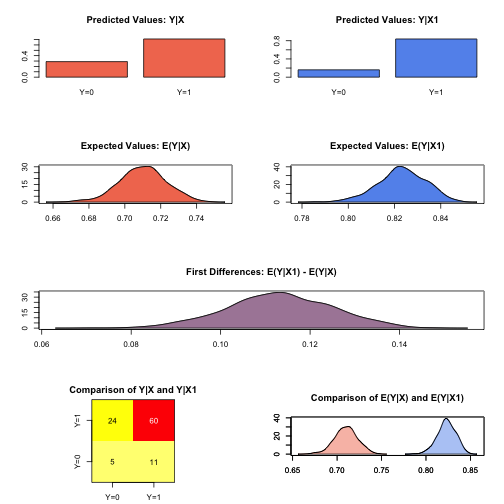
\includegraphics{Zelig-lognorm-1.png}
\caption{Zelig-lognorm}\end{figure}


\paragraph{Model}
\label{zelig-lognorm:model}
Let \(Y_i^*\) be the survival time for observation \(i\) with
the density function \(f(y)\) and the corresponding distribution
function \(F(t)=\int_{0}^t f(y) dy\). This variable might be
censored for some observations at a fixed time \(y_c\) such that the
fully observed dependent variable, \(Y_i\), is defined as
\begin{gather}
\begin{split}Y_i = \left\{ \begin{array}{ll}
      Y_i^* & \textrm{if }Y_i^* \leq y_c \\
      y_c & \textrm{if }Y_i^* > y_c \\
    \end{array} \right.\end{split}\notag
\end{gather}\begin{itemize}
\item {} 
The \emph{stochastic component} is described by the distribution of the
partially observed variable, \(Y^*\). For the lognormal model,
there are two equivalent representations:
\begin{gather}
\begin{split}\begin{aligned}
    Y_i^* \; \sim \; \textrm{LogNormal}(\mu_i, \sigma^2) & \textrm{ or
} & \log(Y_i^*) \; \sim \; \textrm{Normal}(\mu_i, \sigma^2)\end{aligned}\end{split}\notag
\end{gather}
where the parameters \(\mu_i\) and \(\sigma^2\) are the mean
and variance of the Normal distribution. (Note that the output from
zelig() parameterizes scale:math:{}` = sigma{}`.)

In addition, survival models like the lognormal have three additional
properties. The hazard function \(h(t)\) measures the probability
of not surviving past time \(t\) given survival up to \(t\).
In general, the hazard function is equal to \(f(t)/S(t)\) where
the survival function \(S(t) =1 - \int_{0}^t f(s) ds\) represents the fraction still surviving at
time \(t\). The cumulative hazard function \(H(t)\) describes
the probability of dying before time \(t\). In general,
\(H(t)=
\int_{0}^{t} h(s) ds = -\log S(t)\). In the case of the lognormal
model,
\begin{gather}
\begin{split}\begin{aligned}
h(t) &=& \frac{1}{\sqrt{2 \pi} \, \sigma t \, S(t)}
\exp\left\{-\frac{1}{2 \sigma^2} (\log \lambda t)^2\right\} \\
S(t) &=& 1 - \Phi\left(\frac{1}{\sigma} \log \lambda t\right) \\
H(t) &=& -\log \left\{ 1 - \Phi\left(\frac{1}{\sigma} \log \lambda t\right) \right\}\end{aligned}\end{split}\notag
\end{gather}
where \(\Phi(\cdot)\) is the cumulative density function for the
Normal distribution.

\item {} 
The \emph{systematic component} is described as:
\begin{gather}
\begin{split}\mu_i = x_i \beta .\end{split}\notag
\end{gather}
\end{itemize}


\paragraph{Quantities of Interest}
\label{zelig-lognorm:quantities-of-interest}\begin{itemize}
\item {} 
The expected values (qi\$ev) for the lognormal model are simulations
of the expected duration:
\begin{gather}
\begin{split}E(Y) =  \exp\left(\mu_i + \frac{1}{2}\sigma^2 \right),\end{split}\notag
\end{gather}
given draws of \(\beta\) and \(\sigma\) from their sampling
distributions.

\item {} 
The predicted value is a draw from the log-normal distribution given
simulations of the parameters \((\lambda_i, \sigma)\).

\item {} 
The first difference (qi\$fd) is
\begin{gather}
\begin{split}\textrm{FD} = E(Y \mid x_1) - E(Y \mid x).\end{split}\notag
\end{gather}
\item {} 
In conditional prediction models, the average expected treatment
effect (att.ev) for the treatment group is
\begin{gather}
\begin{split}\frac{1}{\sum_{i=1}^n t_i}\sum_{i:t_i=1}^n \{ Y_i(t_i=1) - E[Y_i(t_i=0)] \},\end{split}\notag
\end{gather}
where \(t_i\) is a binary explanatory variable defining the
treatment (\(t_i=1\)) and control (\(t_i=0\)) groups. When
\(Y_i(t_i=1)\) is censored rather than observed, we replace it
with a simulation from the model given available knowledge of the
censoring process. Variation in the simulations is due to two
factors: uncertainty in the imputation process for censored
\(y_i^*\) and uncertainty in simulating \(E[Y_i(t_i=0)]\),
the counterfactual expected value of \(Y_i\) for observations in
the treatment group, under the assumption that everything stays the
same except that the treatment indicator is switched to
\(t_i=0\).

\item {} 
In conditional prediction models, the average predicted treatment
effect (att.pr) for the treatment group is
\begin{gather}
\begin{split}\frac{1}{\sum_{i=1}^n t_i} \sum_{i:t_i=1}^n \{  Y_i(t_i=1) -
\widehat{Y_i(t_i=0)} \},\end{split}\notag
\end{gather}
where \(t_i\) is a binary explanatory variable defining the
treatment (\(t_i=1\)) and control (\(t_i=0\)) groups. When
\(Y_i(t_i=1)\) is censored rather than observed, we replace it
with a simulation from the model given available knowledge of the
censoring process. Variation in the simulations are due to two
factors: uncertainty in the imputation process for censored
\(y_i^*\) and uncertainty in simulating
\(\widehat{Y_i(t_i=0)}\), the counterfactual predicted value of
\(Y_i\) for observations in the treatment group, under the
assumption that everything stays the same except that the treatment
indicator is switched to \(t_i=0\).

\end{itemize}


\paragraph{Output Values}
\label{zelig-lognorm:output-values}
The output of each Zelig command contains useful information which you
may view. For example, if you run
\code{z.out \textless{}- zelig(Surv(Y, C) \textasciitilde{} X, model = lognorm, data)}, then you may
examine the available information in \code{z.out} by using
\code{names(z.out)}, see the coefficients by using z.out\$coefficients, and
a default summary of information through \code{summary(z.out)}.


\paragraph{See also}
\label{zelig-lognorm:see-also}
The exponential function is part of the survival library by by Terry
Therneau, ported to R by Thomas Lumley. Advanced users may wish to refer
to \code{help(survfit)} in the survival library.


\subsubsection{zelig-ls}
\label{zelig-ls::doc}\label{zelig-ls:zelig-ls}\label{zelig-ls:zls}
Least Squares Regression for Continuous Dependent Variables

Use least squares regression analysis to estimate the best linear
predictor for the specified dependent variables.


\paragraph{Syntax}
\label{zelig-ls:syntax}
With reference classes:

\begin{Verbatim}[commandchars=\\\{\}]
z5 \PYG{o}{\PYGZlt{}\PYGZhy{}} zls\PYG{o}{\PYGZdl{}}new\PYG{p}{(}\PYG{p}{)}
z5\PYG{o}{\PYGZdl{}}zelig\PYG{p}{(}Y \PYG{o}{\PYGZti{}} X1 \PYG{o}{+} X \PYG{o}{\PYGZti{}} X\PYG{p}{,} data \PYG{o}{=} mydata\PYG{p}{)}
z5\PYG{o}{\PYGZdl{}}setx\PYG{p}{(}\PYG{p}{)}
z5\PYG{o}{\PYGZdl{}}sim\PYG{p}{(}\PYG{p}{)}
\end{Verbatim}

With the Zelig 4 compatibility wrappers:

\begin{Verbatim}[commandchars=\\\{\}]
z.out \PYG{o}{\PYGZlt{}\PYGZhy{}} zelig\PYG{p}{(}Y \PYG{o}{\PYGZti{}} X1 \PYG{o}{+} X2\PYG{p}{,} model \PYG{o}{=} \PYG{l+s}{\PYGZdq{}}\PYG{l+s}{ls\PYGZdq{}}\PYG{p}{,} data \PYG{o}{=} mydata\PYG{p}{)}
x.out \PYG{o}{\PYGZlt{}\PYGZhy{}} setx\PYG{p}{(}z.out\PYG{p}{)}
s.out \PYG{o}{\PYGZlt{}\PYGZhy{}} sim\PYG{p}{(}z.out\PYG{p}{,} x \PYG{o}{=} x.out\PYG{p}{)}
\end{Verbatim}


\paragraph{Examples}
\label{zelig-ls:examples}

\subparagraph{Basic Example with First Differences}
\label{zelig-ls:basic-example-with-first-differences}
Attach sample data:

\begin{Verbatim}[commandchars=\\\{\}]
data\PYG{p}{(}macro\PYG{p}{)}
\end{Verbatim}

Estimate model:

\begin{Verbatim}[commandchars=\\\{\}]
z.out1 \PYG{o}{\PYGZlt{}\PYGZhy{}} zelig\PYG{p}{(}unem \PYG{o}{\PYGZti{}} gdp \PYG{o}{+} capmob \PYG{o}{+} trade\PYG{p}{,} model \PYG{o}{=} \PYG{l+s}{\PYGZdq{}}\PYG{l+s}{ls\PYGZdq{}}\PYG{p}{,} data \PYG{o}{=} macro\PYG{p}{)}
\end{Verbatim}

\begin{Verbatim}[commandchars=\\\{\}]
\PYG{c}{\PYGZsh{}\PYGZsh{} How to cite this model in Zelig:}
\PYG{c}{\PYGZsh{}\PYGZsh{}   Kosuke Imai, Gary King, and Olivia Lau. 2007.}
\PYG{c}{\PYGZsh{}\PYGZsh{}   ls: Least Squares Regression for Continuous Dependent Variables}
\PYG{c}{\PYGZsh{}\PYGZsh{}   in Kosuke Imai, Gary King, and Olivia Lau, \PYGZdq{}Zelig: Everyone\PYGZsq{}s Statistical Software,\PYGZdq{}}
\PYG{c}{\PYGZsh{}\PYGZsh{}   http://zeligproject.org/}
\end{Verbatim}

Summarize regression coefficients:

\begin{Verbatim}[commandchars=\\\{\}]
summary\PYG{p}{(}z.out1\PYG{p}{)}
\end{Verbatim}

\begin{Verbatim}[commandchars=\\\{\}]
\PYG{c}{\PYGZsh{}\PYGZsh{} Model:}
\PYG{c}{\PYGZsh{}\PYGZsh{} \PYGZdl{}by}
\PYG{c}{\PYGZsh{}\PYGZsh{} [1] 1}
\PYG{c}{\PYGZsh{}\PYGZsh{}}
\PYG{c}{\PYGZsh{}\PYGZsh{}}
\PYG{c}{\PYGZsh{}\PYGZsh{} Call:}
\PYG{c}{\PYGZsh{}\PYGZsh{} stats::lm(formula = unem \PYGZti{} gdp + capmob + trade, data = .)}
\PYG{c}{\PYGZsh{}\PYGZsh{}}
\PYG{c}{\PYGZsh{}\PYGZsh{} Coefficients:}
\PYG{c}{\PYGZsh{}\PYGZsh{} (Intercept)          gdp       capmob        trade}
\PYG{c}{\PYGZsh{}\PYGZsh{}     6.18129     \PYGZhy{}0.32360      1.42194      0.01985}
\PYG{c}{\PYGZsh{}\PYGZsh{}}
\PYG{c}{\PYGZsh{}\PYGZsh{} Next step: Use \PYGZsq{}setx\PYGZsq{} method}
\end{Verbatim}

Set explanatory variables to their default (mean/mode) values, with
high (80th percentile) and low (20th percentile) values for the trade
variable:

\begin{Verbatim}[commandchars=\\\{\}]
x.high \PYG{o}{\PYGZlt{}\PYGZhy{}} setx\PYG{p}{(}z.out1\PYG{p}{,} trade \PYG{o}{=} quantile\PYG{p}{(}macro\PYG{o}{\PYGZdl{}}trade\PYG{p}{,} \PYG{l+m}{0.8}\PYG{p}{)}\PYG{p}{)}
x.low \PYG{o}{\PYGZlt{}\PYGZhy{}} setx\PYG{p}{(}z.out1\PYG{p}{,} trade \PYG{o}{=} quantile\PYG{p}{(}macro\PYG{o}{\PYGZdl{}}trade\PYG{p}{,} \PYG{l+m}{0.2}\PYG{p}{)}\PYG{p}{)}
\end{Verbatim}

Generate first differences for the effect of high versus low trade on GDP:

\begin{Verbatim}[commandchars=\\\{\}]
s.out1 \PYG{o}{\PYGZlt{}\PYGZhy{}} sim\PYG{p}{(}z.out1\PYG{p}{,} x \PYG{o}{=} x.high\PYG{p}{,} x1 \PYG{o}{=} x.low\PYG{p}{)}
\end{Verbatim}

\begin{Verbatim}[commandchars=\\\{\}]
summary\PYG{p}{(}s.out1\PYG{p}{)}
\end{Verbatim}

\begin{Verbatim}[commandchars=\\\{\}]
\PYG{c}{\PYGZsh{}\PYGZsh{}}
\PYG{c}{\PYGZsh{}\PYGZsh{}  sim x :}
\PYG{c}{\PYGZsh{}\PYGZsh{}  \PYGZhy{}\PYGZhy{}\PYGZhy{}\PYGZhy{}\PYGZhy{}}
\PYG{c}{\PYGZsh{}\PYGZsh{} ev}
\PYG{c}{\PYGZsh{}\PYGZsh{}       mean        sd      50\PYGZpc{}     2.5\PYGZpc{}    97.5\PYGZpc{}}
\PYG{c}{\PYGZsh{}\PYGZsh{} 1 5.430307 0.1971789 5.431243 5.038718 5.815665}
\PYG{c}{\PYGZsh{}\PYGZsh{} pv}
\PYG{c}{\PYGZsh{}\PYGZsh{}       mean        sd      50\PYGZpc{}     2.5\PYGZpc{}    97.5\PYGZpc{}}
\PYG{c}{\PYGZsh{}\PYGZsh{} 1 5.430307 0.1971789 5.431243 5.038718 5.815665}
\PYG{c}{\PYGZsh{}\PYGZsh{}}
\PYG{c}{\PYGZsh{}\PYGZsh{}  sim x1 :}
\PYG{c}{\PYGZsh{}\PYGZsh{}  \PYGZhy{}\PYGZhy{}\PYGZhy{}\PYGZhy{}\PYGZhy{}}
\PYG{c}{\PYGZsh{}\PYGZsh{} ev}
\PYG{c}{\PYGZsh{}\PYGZsh{}       mean        sd      50\PYGZpc{}    2.5\PYGZpc{}    97.5\PYGZpc{}}
\PYG{c}{\PYGZsh{}\PYGZsh{} 1 4.602931 0.1804596 4.604509 4.23388 4.957203}
\PYG{c}{\PYGZsh{}\PYGZsh{} pv}
\PYG{c}{\PYGZsh{}\PYGZsh{}       mean        sd      50\PYGZpc{}    2.5\PYGZpc{}    97.5\PYGZpc{}}
\PYG{c}{\PYGZsh{}\PYGZsh{} 1 4.602931 0.1804596 4.604509 4.23388 4.957203}
\PYG{c}{\PYGZsh{}\PYGZsh{} fd}
\PYG{c}{\PYGZsh{}\PYGZsh{}         mean        sd        50\PYGZpc{}      2.5\PYGZpc{}      97.5\PYGZpc{}}
\PYG{c}{\PYGZsh{}\PYGZsh{} 1 \PYGZhy{}0.8273756 0.2379988 \PYGZhy{}0.8281937 \PYGZhy{}1.295583 \PYGZhy{}0.3443534}
\end{Verbatim}

\begin{Verbatim}[commandchars=\\\{\}]
plot\PYG{p}{(}s.out1\PYG{p}{)}
\end{Verbatim}
\begin{figure}[htbp]
\centering

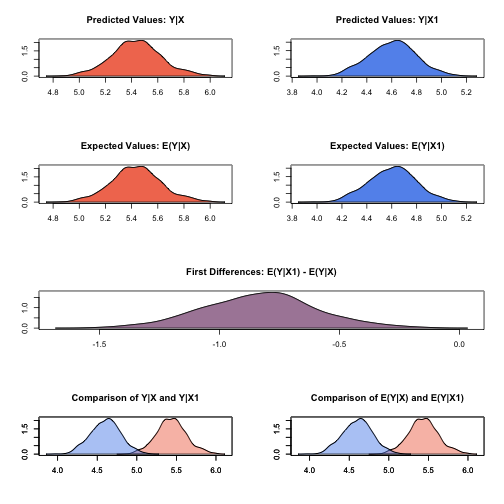
\includegraphics{unnamed-chunk-10-1.png}
\end{figure}


\subparagraph{Using Dummy Variables}
\label{zelig-ls:using-dummy-variables}
Estimate a model with fixed effects for each country (see for help
with dummy variables). Note that you do not need to create dummy
variables, as the program will automatically parse the unique values
in the selected variable into discrete levels.

\begin{Verbatim}[commandchars=\\\{\}]
z.out2 \PYG{o}{\PYGZlt{}\PYGZhy{}} zelig\PYG{p}{(}unem \PYG{o}{\PYGZti{}} gdp \PYG{o}{+} trade \PYG{o}{+} capmob \PYG{o}{+} as.factor\PYG{p}{(}country\PYG{p}{)}\PYG{p}{,} model \PYG{o}{=} \PYG{l+s}{\PYGZdq{}}\PYG{l+s}{ls\PYGZdq{}}\PYG{p}{,} data \PYG{o}{=} macro\PYG{p}{)}
\end{Verbatim}

\begin{Verbatim}[commandchars=\\\{\}]
\PYG{c}{\PYGZsh{}\PYGZsh{} How to cite this model in Zelig:}
\PYG{c}{\PYGZsh{}\PYGZsh{}   Kosuke Imai, Gary King, and Olivia Lau. 2007.}
\PYG{c}{\PYGZsh{}\PYGZsh{}   ls: Least Squares Regression for Continuous Dependent Variables}
\PYG{c}{\PYGZsh{}\PYGZsh{}   in Kosuke Imai, Gary King, and Olivia Lau, \PYGZdq{}Zelig: Everyone\PYGZsq{}s Statistical Software,\PYGZdq{}}
\PYG{c}{\PYGZsh{}\PYGZsh{}   http://zeligproject.org/}
\end{Verbatim}

Set values for the explanatory variables, using the default mean/mode
values, with country set to the United States and Japan,
respectively:

\begin{Verbatim}[commandchars=\\\{\}]
x.US \PYG{o}{\PYGZlt{}\PYGZhy{}} setx\PYG{p}{(}z.out2\PYG{p}{,} country \PYG{o}{=} \PYG{l+s}{\PYGZdq{}}\PYG{l+s}{United States\PYGZdq{}}\PYG{p}{)}
x.Japan \PYG{o}{\PYGZlt{}\PYGZhy{}} setx\PYG{p}{(}z.out2\PYG{p}{,} country \PYG{o}{=} \PYG{l+s}{\PYGZdq{}}\PYG{l+s}{Japan\PYGZdq{}}\PYG{p}{)}
\end{Verbatim}

Simulate quantities of interest:

\begin{Verbatim}[commandchars=\\\{\}]
s.out2 \PYG{o}{\PYGZlt{}\PYGZhy{}} sim\PYG{p}{(}z.out2\PYG{p}{,} x \PYG{o}{=} x.US\PYG{p}{,} x1 \PYG{o}{=} x.Japan\PYG{p}{)}
\end{Verbatim}

\begin{Verbatim}[commandchars=\\\{\}]
plot\PYG{p}{(}s.out2\PYG{p}{)}
\end{Verbatim}
\begin{figure}[htbp]
\centering

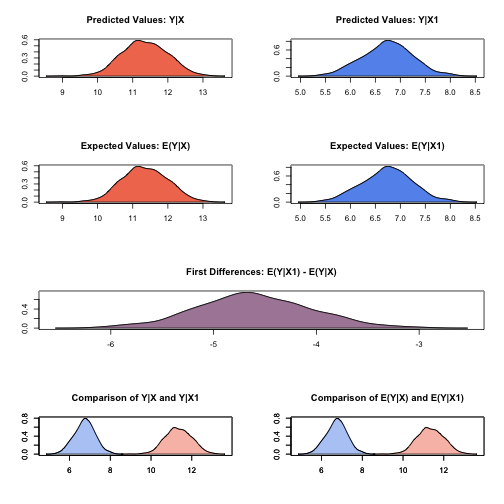
\includegraphics{unnamed-chunk-14-1.png}
\end{figure}


\paragraph{Model}
\label{zelig-ls:model}\begin{itemize}
\item {} 
The \emph{stochastic component} is described by a density with mean
\(\mu_i\) and the common variance \(\sigma^2\)
\begin{gather}
\begin{split}Y_i \; \sim \; f(y_i \mid \mu_i, \sigma^2).\end{split}\notag
\end{gather}
\item {} 
The \emph{systematic component} models the conditional mean as
\begin{gather}
\begin{split}\mu_i =  x_i \beta\end{split}\notag
\end{gather}
where \(x_i\) is the vector of covariates, and \(\beta\) is
the vector of coefficients.

The least squares estimator is the best linear predictor of a
dependent variable given \(x_i\), and minimizes the sum of
squared residuals, \(\sum_{i=1}^n (Y_i-x_i \beta)^2\).

\end{itemize}


\paragraph{Quantities of Interest}
\label{zelig-ls:quantities-of-interest}\begin{itemize}
\item {} 
The expected value (qi\$ev) is the mean of simulations from the
stochastic component,
\begin{gather}
\begin{split}E(Y) = x_i \beta,\end{split}\notag
\end{gather}
given a draw of \(\beta\) from its sampling distribution.

\item {} 
In conditional prediction models, the average expected treatment
effect (att.ev) for the treatment group is
\begin{gather}
\begin{split}\frac{1}{\sum_{i=1}^n t_i}\sum_{i:t_i=1}^n \left\{ Y_i(t_i=1) -
      E[Y_i(t_i=0)] \right\},\end{split}\notag
\end{gather}
where \(t_i\) is a binary explanatory variable defining the
treatment (\(t_i=1\)) and control (\(t_i=0\)) groups.
Variation in the simulations are due to uncertainty in simulating
\(E[Y_i(t_i=0)]\), the counterfactual expected value of
\(Y_i\) for observations in the treatment group, under the
assumption that everything stays the same except that the treatment
indicator is switched to \(t_i=0\).

\end{itemize}


\paragraph{Output Values}
\label{zelig-ls:output-values}
The output of each Zelig command contains useful information which you
may view. For example, if you run
\code{z.out \textless{}- zelig(y \textasciitilde{} x, model = ls, data)}, then you may examine the
available information in \code{z.out} by using \code{names(z.out)}, see the
coefficients by using z.out\$coefficients, and a default summary of
information through \code{summary(z.out)}. Other elements available through
the \$ operator are listed below.
\begin{itemize}
\item {} 
From the zelig() output object z.out, you may extract:
\begin{itemize}
\item {} 
coefficients: parameter estimates for the explanatory variables.

\item {} 
residuals: the working residuals in the final iteration of the
IWLS fit.

\item {} 
fitted.values: fitted values.

\item {} 
df.residual: the residual degrees of freedom.

\item {} 
zelig.data: the input data frame if save.data = TRUE.

\end{itemize}

\item {} 
From summary(z.out), you may extract:
\begin{itemize}
\item {} 
coefficients: the parameter estimates with their associated
standard errors, \(p\)-values, and \(t\)-statistics.
\begin{gather}
\begin{split}\hat{\beta} \; = \; \left(\sum_{i=1}^n x_i' x_i\right)^{-1} \sum x_i y_i\end{split}\notag
\end{gather}
\item {} 
sigma: the square root of the estimate variance of the random
error \(e\):
\begin{gather}
\begin{split}\hat{\sigma} \; = \; \frac{\sum (Y_i-x_i\hat{\beta})^2}{n-k}\end{split}\notag
\end{gather}
\item {} 
r.squared: the fraction of the variance explained by the model.
\begin{gather}
\begin{split}R^2 \; = \; 1 - \frac{\sum (Y_i-x_i\hat{\beta})^2}{\sum (y_i -
         \bar{y})^2}\end{split}\notag
\end{gather}
\item {} 
adj.r.squared: the above \(R^2\) statistic, penalizing for an
increased number of explanatory variables.

\item {} 
cov.unscaled: a \(k \times k\) matrix of unscaled covariances.

\end{itemize}

\end{itemize}


\paragraph{See also}
\label{zelig-ls:see-also}
The least squares regression is part of the stats package by William N.
Venables and Brian D. Ripley .In addition, advanced users may wish to
refer to \code{help(lm)} and \code{help(lm.fit)}.


\subsubsection{zelig-negbin}
\label{zelig-negbin:znegbin}\label{zelig-negbin::doc}\label{zelig-negbin:zelig-negbin}
Negative Binomial Regression for Event Count Dependent Variables

Use the negative binomial regression if you have a count of events for
each observation of your dependent variable. The negative binomial model
is frequently used to estimate over-dispersed event count models.


\paragraph{Syntax}
\label{zelig-negbin:syntax}
With reference classes:

\begin{Verbatim}[commandchars=\\\{\}]
z5 \PYG{o}{\PYGZlt{}\PYGZhy{}} znegbin\PYG{o}{\PYGZdl{}}new\PYG{p}{(}\PYG{p}{)}
z5\PYG{o}{\PYGZdl{}}zelig\PYG{p}{(}Y \PYG{o}{\PYGZti{}} X1 \PYG{o}{+} X \PYG{o}{\PYGZti{}} X\PYG{p}{,} data \PYG{o}{=} mydata\PYG{p}{)}
z5\PYG{o}{\PYGZdl{}}setx\PYG{p}{(}\PYG{p}{)}
z5\PYG{o}{\PYGZdl{}}sim\PYG{p}{(}\PYG{p}{)}
\end{Verbatim}

With the Zelig 4 compatibility wrappers:

\begin{Verbatim}[commandchars=\\\{\}]
z.out \PYG{o}{\PYGZlt{}\PYGZhy{}} zelig\PYG{p}{(}Y \PYG{o}{\PYGZti{}} X1 \PYG{o}{+} X2\PYG{p}{,} model \PYG{o}{=} \PYG{l+s}{\PYGZdq{}}\PYG{l+s}{negbin\PYGZdq{}}\PYG{p}{,} data \PYG{o}{=} mydata\PYG{p}{)}
x.out \PYG{o}{\PYGZlt{}\PYGZhy{}} setx\PYG{p}{(}z.out\PYG{p}{)}
s.out \PYG{o}{\PYGZlt{}\PYGZhy{}} sim\PYG{p}{(}z.out\PYG{p}{,} x \PYG{o}{=} x.out\PYG{p}{)}
\end{Verbatim}


\paragraph{Example}
\label{zelig-negbin:example}
Load sample data:

\begin{Verbatim}[commandchars=\\\{\}]
data\PYG{p}{(}sanction\PYG{p}{)}
\end{Verbatim}

Estimate the model:

\begin{Verbatim}[commandchars=\\\{\}]
z.out \PYG{o}{\PYGZlt{}\PYGZhy{}} zelig\PYG{p}{(}num \PYG{o}{\PYGZti{}} target \PYG{o}{+} coop\PYG{p}{,} model \PYG{o}{=} \PYG{l+s}{\PYGZdq{}}\PYG{l+s}{negbin\PYGZdq{}}\PYG{p}{,} data \PYG{o}{=} sanction\PYG{p}{)}
\end{Verbatim}

\begin{Verbatim}[commandchars=\\\{\}]
\PYG{c}{\PYGZsh{}\PYGZsh{} How to cite this model in Zelig:}
\PYG{c}{\PYGZsh{}\PYGZsh{}   Kosuke Imai, Gary King, Olivia Lau. 2008.}
\PYG{c}{\PYGZsh{}\PYGZsh{}   negbinom: Negative Binomial Regression for Event Count Dependent Variables}
\PYG{c}{\PYGZsh{}\PYGZsh{}   in Kosuke Imai, Gary King, and Olivia Lau, \PYGZdq{}Zelig: Everyone\PYGZsq{}s Statistical Software,\PYGZdq{}}
\PYG{c}{\PYGZsh{}\PYGZsh{}   http://zeligproject.org/}
\end{Verbatim}

\begin{Verbatim}[commandchars=\\\{\}]
summary\PYG{p}{(}z.out\PYG{p}{)}
\end{Verbatim}

\begin{Verbatim}[commandchars=\\\{\}]
\PYG{c}{\PYGZsh{}\PYGZsh{} Model:}
\PYG{c}{\PYGZsh{}\PYGZsh{} \PYGZdl{}by}
\PYG{c}{\PYGZsh{}\PYGZsh{} [1] 1}
\PYG{c}{\PYGZsh{}\PYGZsh{}}
\PYG{c}{\PYGZsh{}\PYGZsh{}}
\PYG{c}{\PYGZsh{}\PYGZsh{} Call:  MASS::glm.nb(formula = num \PYGZti{} target + coop, data = ., init.theta = 1.841603403,}
\PYG{c}{\PYGZsh{}\PYGZsh{}     link = log)}
\PYG{c}{\PYGZsh{}\PYGZsh{}}
\PYG{c}{\PYGZsh{}\PYGZsh{} Coefficients:}
\PYG{c}{\PYGZsh{}\PYGZsh{} (Intercept)       target         coop}
\PYG{c}{\PYGZsh{}\PYGZsh{}      \PYGZhy{}1.564        0.151        1.286}
\PYG{c}{\PYGZsh{}\PYGZsh{}}
\PYG{c}{\PYGZsh{}\PYGZsh{} Degrees of Freedom: 77 Total (i.e. Null);  75 Residual}
\PYG{c}{\PYGZsh{}\PYGZsh{} Null Deviance:       237.1}
\PYG{c}{\PYGZsh{}\PYGZsh{} Residual Deviance: 56.55         AIC: 360.2}
\PYG{c}{\PYGZsh{}\PYGZsh{} Next step: Use \PYGZsq{}setx\PYGZsq{} method}
\end{Verbatim}

Set values for the explanatory variables to their default mean values:

\begin{Verbatim}[commandchars=\\\{\}]
x.out \PYG{o}{\PYGZlt{}\PYGZhy{}} setx\PYG{p}{(}z.out\PYG{p}{)}
\end{Verbatim}

Simulate fitted values:

\begin{Verbatim}[commandchars=\\\{\}]
s.out \PYG{o}{\PYGZlt{}\PYGZhy{}} sim\PYG{p}{(}z.out\PYG{p}{,} x \PYG{o}{=} x.out\PYG{p}{)}
\end{Verbatim}

\begin{Verbatim}[commandchars=\\\{\}]
summary\PYG{p}{(}s.out\PYG{p}{)}
\end{Verbatim}

\begin{Verbatim}[commandchars=\\\{\}]
\PYG{c}{\PYGZsh{}\PYGZsh{}}
\PYG{c}{\PYGZsh{}\PYGZsh{}  sim x :}
\PYG{c}{\PYGZsh{}\PYGZsh{}  \PYGZhy{}\PYGZhy{}\PYGZhy{}\PYGZhy{}\PYGZhy{}}
\PYG{c}{\PYGZsh{}\PYGZsh{} ev}
\PYG{c}{\PYGZsh{}\PYGZsh{}          mean       sd      50\PYGZpc{}     2.5\PYGZpc{}    97.5\PYGZpc{}}
\PYG{c}{\PYGZsh{}\PYGZsh{} [1,] 2.948528 0.360773 2.916141 2.323829 3.703429}
\PYG{c}{\PYGZsh{}\PYGZsh{} pv}
\PYG{c}{\PYGZsh{}\PYGZsh{} qi}
\PYG{c}{\PYGZsh{}\PYGZsh{}     0     1     2     3     4     5     6     7     8     9    10    11}
\PYG{c}{\PYGZsh{}\PYGZsh{} 0.193 0.189 0.186 0.134 0.095 0.064 0.045 0.036 0.026 0.007 0.007 0.009}
\PYG{c}{\PYGZsh{}\PYGZsh{}    12    13    14    15    16    17    30}
\PYG{c}{\PYGZsh{}\PYGZsh{} 0.002 0.001 0.001 0.002 0.001 0.001 0.001}
\end{Verbatim}

\begin{Verbatim}[commandchars=\\\{\}]
plot\PYG{p}{(}s.out\PYG{p}{)}
\end{Verbatim}
\begin{figure}[htbp]
\centering
\capstart

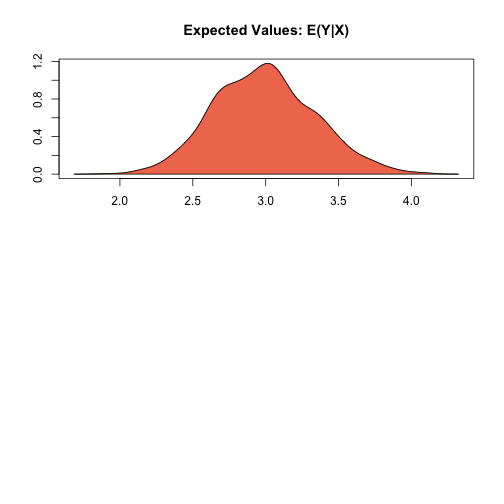
\includegraphics{Zelig-negbin-1.png}
\caption{Zelig-negbin}\end{figure}


\paragraph{Model}
\label{zelig-negbin:model}
Let \(Y_i\) be the number of independent events that occur during a
fixed time period. This variable can take any non-negative integer
value.
\begin{itemize}
\item {} 
The negative binomial distribution is derived by letting the mean of
the Poisson distribution vary according to a fixed parameter
\(\zeta\) given by the Gamma distribution. The \emph{stochastic
component} is given by
\begin{gather}
\begin{split}\begin{aligned}
     Y_i \mid \zeta_i & \sim & \textrm{Poisson}(\zeta_i \mu_i),\\
     \zeta_i & \sim & \frac{1}{\theta}\textrm{Gamma}(\theta).
   \end{aligned}\end{split}\notag
\end{gather}
The marginal distribution of \(Y_i\) is then the negative
binomial with mean \(\mu_i\) and variance
\(\mu_i + \mu_i^2/\theta\):
\begin{gather}
\begin{split}\begin{aligned}
   Y_i & \sim & \textrm{NegBin}(\mu_i, \theta), \\
       & = & \frac{\Gamma (\theta + y_i)}{y! \, \Gamma(\theta)}
             \frac{\mu_i^{y_i} \, \theta^{\theta}}{(\mu_i + \theta)^{\theta + y_i}},
   \end{aligned}\end{split}\notag
\end{gather}
where \(\theta\) is the systematic parameter of the Gamma
distribution modeling \(\zeta_i\).

\item {} 
The \emph{systematic component} is given by
\begin{gather}
\begin{split}\mu_i = \exp(x_i \beta)\end{split}\notag
\end{gather}
where \(x_i\) is the vector of \(k\) explanatory variables
and \(\beta\) is the vector of coefficients.

\end{itemize}


\paragraph{Quantities of Interest}
\label{zelig-negbin:quantities-of-interest}\begin{itemize}
\item {} 
The expected values (qi\$ev) are simulations of the mean of the
stochastic component. Thus,
\begin{gather}
\begin{split}E(Y) = \mu_i = \exp(x_i
  \beta),\end{split}\notag
\end{gather}
given simulations of \(\beta\).

\item {} 
The predicted value (qi\$pr) drawn from the distribution defined by
the set of parameters \((\mu_i, \theta)\).

\item {} 
The first difference (qi\$fd) is
\begin{gather}
\begin{split}\textrm{FD} \; = \; E(Y | x_1) - E(Y \mid x)\end{split}\notag
\end{gather}
\item {} 
In conditional prediction models, the average expected treatment
effect (att.ev) for the treatment group is
\begin{gather}
\begin{split}\frac{1}{\sum_{i=1}^n t_i}\sum_{i:t_i=1}^n \left\{ Y_i(t_i=1) -
      E[Y_i(t_i=0)] \right\},\end{split}\notag
\end{gather}
where \(t_i\) is a binary explanatory variable defining the
treatment (\(t_i=1\)) and control (\(t_i=0\)) groups.
Variation in the simulations are due to uncertainty in simulating
\(E[Y_i(t_i=0)]\), the counterfactual expected value of
\(Y_i\) for observations in the treatment group, under the
assumption that everything stays the same except that the treatment
indicator is switched to \(t_i=0\).

\item {} 
In conditional prediction models, the average predicted treatment
effect (att.pr) for the treatment group is
\begin{gather}
\begin{split}\frac{1}{\sum_{i=1}^n t_i}\sum_{i:t_i=1}^n \left\{ Y_i(t_i=1) -
      \widehat{Y_i(t_i=0)} \right\},\end{split}\notag
\end{gather}
where \(t_i\) is a binary explanatory variable defining the
treatment (\(t_i=1\)) and control (\(t_i=0\)) groups.
Variation in the simulations are due to uncertainty in simulating
\(\widehat{Y_i(t_i=0)}\), the counterfactual predicted value of
\(Y_i\) for observations in the treatment group, under the
assumption that everything stays the same except that the treatment
indicator is switched to \(t_i=0\).

\end{itemize}


\paragraph{Output Values}
\label{zelig-negbin:output-values}
The output of each Zelig command contains useful information which you
may view. For example, if you run
\code{z.out \textless{}- zelig(y \textasciitilde{} x, model = negbin, data)}, then you may examine
the available information in \code{z.out} by using \code{names(z.out)}, see
the coefficients by using z.out\$coefficients, and a default summary of
information through \code{summary(z.out)}.


\paragraph{See also}
\label{zelig-negbin:see-also}
The negative binomial model is part of the MASS package by William N.
Venable and Brian D. Ripley . Advanced users may wish to refer to
{\color{red}\bfseries{}{}`{}`}help(glm.nb){}`.


\subsubsection{zelig-normal}
\label{zelig-normal:zelig-normal}\label{zelig-normal::doc}\label{zelig-normal:znorm}
Normal Regression for Continuous Dependent Variables

The Normal regression model is a close variant of the more standard
least squares regression model (see ). Both models specify a continuous
dependent variable as a linear function of a set of explanatory
variables. The Normal model reports maximum likelihood (rather than
least squares) estimates. The two models differ only in their estimate
for the stochastic parameter \(\sigma\).


\paragraph{Syntax}
\label{zelig-normal:syntax}
With reference classes:

\begin{Verbatim}[commandchars=\\\{\}]
z5 \PYG{o}{\PYGZlt{}\PYGZhy{}} znormal\PYG{o}{\PYGZdl{}}new\PYG{p}{(}\PYG{p}{)}
z5\PYG{o}{\PYGZdl{}}zelig\PYG{p}{(}Y \PYG{o}{\PYGZti{}} X1 \PYG{o}{+} X \PYG{o}{\PYGZti{}} X\PYG{p}{,} data \PYG{o}{=} mydata\PYG{p}{)}
z5\PYG{o}{\PYGZdl{}}setx\PYG{p}{(}\PYG{p}{)}
z5\PYG{o}{\PYGZdl{}}sim\PYG{p}{(}\PYG{p}{)}
\end{Verbatim}

With the Zelig 4 compatibility wrappers:

\begin{Verbatim}[commandchars=\\\{\}]
z.out \PYG{o}{\PYGZlt{}\PYGZhy{}} zelig\PYG{p}{(}Y \PYG{o}{\PYGZti{}} X1 \PYG{o}{+} X2\PYG{p}{,} model \PYG{o}{=} \PYG{l+s}{\PYGZdq{}}\PYG{l+s}{normal\PYGZdq{}}\PYG{p}{,} data \PYG{o}{=} mydata\PYG{p}{)}
x.out \PYG{o}{\PYGZlt{}\PYGZhy{}} setx\PYG{p}{(}z.out\PYG{p}{)}
s.out \PYG{o}{\PYGZlt{}\PYGZhy{}} sim\PYG{p}{(}z.out\PYG{p}{,} x \PYG{o}{=} x.out\PYG{p}{)}
\end{Verbatim}


\paragraph{Examples}
\label{zelig-normal:examples}

\subparagraph{Basic Example with First Differences}
\label{zelig-normal:basic-example-with-first-differences}
Attach sample data:

\begin{Verbatim}[commandchars=\\\{\}]
data\PYG{p}{(}macro\PYG{p}{)}
\end{Verbatim}

Estimate model:

\begin{Verbatim}[commandchars=\\\{\}]
z.out1 \PYG{o}{\PYGZlt{}\PYGZhy{}} zelig\PYG{p}{(}unem \PYG{o}{\PYGZti{}} gdp \PYG{o}{+} capmob \PYG{o}{+} trade\PYG{p}{,} model \PYG{o}{=} \PYG{l+s}{\PYGZdq{}}\PYG{l+s}{normal\PYGZdq{}}\PYG{p}{,} data \PYG{o}{=} macro\PYG{p}{)}
\end{Verbatim}

\begin{Verbatim}[commandchars=\\\{\}]
\PYG{c}{\PYGZsh{}\PYGZsh{} How to cite this model in Zelig:}
\PYG{c}{\PYGZsh{}\PYGZsh{}   Kosuke Imai, Gary King, Olivia Lau. 2008.}
\PYG{c}{\PYGZsh{}\PYGZsh{}   normal: Normal Regression for Continuous Dependent Variables}
\PYG{c}{\PYGZsh{}\PYGZsh{}   in Kosuke Imai, Gary King, and Olivia Lau, \PYGZdq{}Zelig: Everyone\PYGZsq{}s Statistical Software,\PYGZdq{}}
\PYG{c}{\PYGZsh{}\PYGZsh{}   http://zeligproject.org/}
\end{Verbatim}

Summarize of regression coefficients:

\begin{Verbatim}[commandchars=\\\{\}]
summary\PYG{p}{(}z.out1\PYG{p}{)}
\end{Verbatim}

\begin{Verbatim}[commandchars=\\\{\}]
\PYG{c}{\PYGZsh{}\PYGZsh{} Model:}
\PYG{c}{\PYGZsh{}\PYGZsh{} \PYGZdl{}by}
\PYG{c}{\PYGZsh{}\PYGZsh{} [1] 1}
\PYG{c}{\PYGZsh{}\PYGZsh{}}
\PYG{c}{\PYGZsh{}\PYGZsh{}}
\PYG{c}{\PYGZsh{}\PYGZsh{} Call:  stats::glm(formula = unem \PYGZti{} gdp + capmob + trade, family = gaussian(\PYGZdq{}identity\PYGZdq{}),}
\PYG{c}{\PYGZsh{}\PYGZsh{}     data = .)}
\PYG{c}{\PYGZsh{}\PYGZsh{}}
\PYG{c}{\PYGZsh{}\PYGZsh{} Coefficients:}
\PYG{c}{\PYGZsh{}\PYGZsh{} (Intercept)          gdp       capmob        trade}
\PYG{c}{\PYGZsh{}\PYGZsh{}     6.18129     \PYGZhy{}0.32360      1.42194      0.01985}
\PYG{c}{\PYGZsh{}\PYGZsh{}}
\PYG{c}{\PYGZsh{}\PYGZsh{} Degrees of Freedom: 349 Total (i.e. Null);  346 Residual}
\PYG{c}{\PYGZsh{}\PYGZsh{} Null Deviance:       3665}
\PYG{c}{\PYGZsh{}\PYGZsh{} Residual Deviance: 2610  AIC: 1706}
\PYG{c}{\PYGZsh{}\PYGZsh{} Next step: Use \PYGZsq{}setx\PYGZsq{} method}
\end{Verbatim}

Set explanatory variables to their default (mean/mode) values, with
high (80th percentile) and low (20th percentile) values for trade:

\begin{Verbatim}[commandchars=\\\{\}]
x.high \PYG{o}{\PYGZlt{}\PYGZhy{}} setx\PYG{p}{(}z.out1\PYG{p}{,} trade \PYG{o}{=} quantile\PYG{p}{(}macro\PYG{o}{\PYGZdl{}}trade\PYG{p}{,} \PYG{l+m}{0.8}\PYG{p}{)}\PYG{p}{)}
x.low \PYG{o}{\PYGZlt{}\PYGZhy{}} setx\PYG{p}{(}z.out1\PYG{p}{,} trade \PYG{o}{=} quantile\PYG{p}{(}macro\PYG{o}{\PYGZdl{}}trade\PYG{p}{,} \PYG{l+m}{0.2}\PYG{p}{)}\PYG{p}{)}
\end{Verbatim}

Generate first differences for the effect of high versus low trade on GDP:

\begin{Verbatim}[commandchars=\\\{\}]
s.out1 \PYG{o}{\PYGZlt{}\PYGZhy{}} sim\PYG{p}{(}z.out1\PYG{p}{,} x \PYG{o}{=} x.high\PYG{p}{,} x1 \PYG{o}{=} x.low\PYG{p}{)}
\end{Verbatim}

\begin{Verbatim}[commandchars=\\\{\}]
summary\PYG{p}{(}s.out1\PYG{p}{)}
\end{Verbatim}

\begin{Verbatim}[commandchars=\\\{\}]
\PYG{c}{\PYGZsh{}\PYGZsh{}}
\PYG{c}{\PYGZsh{}\PYGZsh{}  sim x :}
\PYG{c}{\PYGZsh{}\PYGZsh{}  \PYGZhy{}\PYGZhy{}\PYGZhy{}\PYGZhy{}\PYGZhy{}}
\PYG{c}{\PYGZsh{}\PYGZsh{} ev}
\PYG{c}{\PYGZsh{}\PYGZsh{}          mean        sd      50\PYGZpc{}     2.5\PYGZpc{}    97.5\PYGZpc{}}
\PYG{c}{\PYGZsh{}\PYGZsh{} [1,] 5.433104 0.1993954 5.432221 5.032391 5.833022}
\PYG{c}{\PYGZsh{}\PYGZsh{} pv}
\PYG{c}{\PYGZsh{}\PYGZsh{}          mean       sd      50\PYGZpc{}       2.5\PYGZpc{}    97.5\PYGZpc{}}
\PYG{c}{\PYGZsh{}\PYGZsh{} [1,] 5.460641 2.736715 5.472975 0.09863579 10.62646}
\PYG{c}{\PYGZsh{}\PYGZsh{}}
\PYG{c}{\PYGZsh{}\PYGZsh{}  sim x1 :}
\PYG{c}{\PYGZsh{}\PYGZsh{}  \PYGZhy{}\PYGZhy{}\PYGZhy{}\PYGZhy{}\PYGZhy{}}
\PYG{c}{\PYGZsh{}\PYGZsh{} ev}
\PYG{c}{\PYGZsh{}\PYGZsh{}          mean        sd      50\PYGZpc{}     2.5\PYGZpc{}    97.5\PYGZpc{}}
\PYG{c}{\PYGZsh{}\PYGZsh{} [1,] 4.602042 0.1755117 4.613065 4.252265 4.945202}
\PYG{c}{\PYGZsh{}\PYGZsh{} pv}
\PYG{c}{\PYGZsh{}\PYGZsh{}          mean       sd      50\PYGZpc{}       2.5\PYGZpc{}    97.5\PYGZpc{}}
\PYG{c}{\PYGZsh{}\PYGZsh{} [1,] 4.767229 2.699091 4.677271 \PYGZhy{}0.5714166 10.08173}
\PYG{c}{\PYGZsh{}\PYGZsh{} fd}
\PYG{c}{\PYGZsh{}\PYGZsh{}           mean        sd        50\PYGZpc{}      2.5\PYGZpc{}      97.5\PYGZpc{}}
\PYG{c}{\PYGZsh{}\PYGZsh{} [1,] \PYGZhy{}0.831062 0.2364614 \PYGZhy{}0.8278868 \PYGZhy{}1.296051 \PYGZhy{}0.3667207}
\end{Verbatim}

A visual summary of quantities of interest:

\begin{Verbatim}[commandchars=\\\{\}]
plot\PYG{p}{(}s.out1\PYG{p}{)}
\end{Verbatim}
\begin{figure}[htbp]
\centering
\capstart

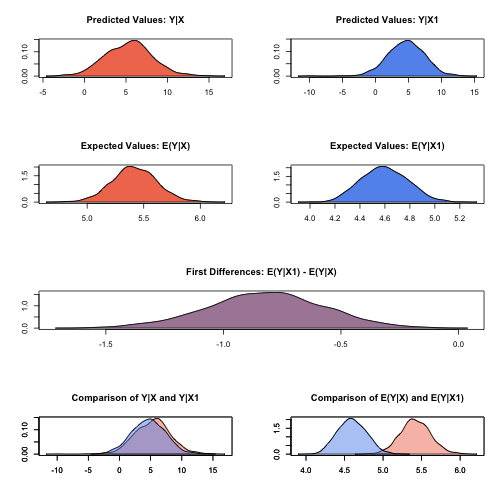
\includegraphics{Zelig-normal-1.png}
\caption{Zelig-normal}\end{figure}


\paragraph{Model}
\label{zelig-normal:model}
Let \(Y_i\) be the continuous dependent variable for observation
\(i\).
\begin{itemize}
\item {} 
The \emph{stochastic component} is described by a univariate normal model
with a vector of means \(\mu_i\) and scalar variance
\(\sigma^2\):
\begin{gather}
\begin{split}Y_i \; \sim \; \textrm{Normal}(\mu_i, \sigma^2).\end{split}\notag
\end{gather}
\item {} 
The \emph{systematic component} is
\begin{gather}
\begin{split}\mu_i \;= \; x_i \beta,\end{split}\notag
\end{gather}
where \(x_i\) is the vector of \(k\) explanatory variables
and \(\beta\) is the vector of coefficients.

\end{itemize}


\paragraph{Quantities of Interest}
\label{zelig-normal:quantities-of-interest}\begin{itemize}
\item {} 
The expected value (qi\$ev) is the mean of simulations from the the
stochastic component,
\begin{gather}
\begin{split}E(Y) = \mu_i = x_i \beta,\end{split}\notag
\end{gather}
given a draw of \(\beta\) from its posterior.

\item {} 
The predicted value (qi\$pr) is drawn from the distribution defined by
the set of parameters \((\mu_i, \sigma)\).

\item {} 
The first difference (qi\$fd) is:
\begin{gather}
\begin{split}\textrm{FD}\; = \;E(Y \mid x_1) -  E(Y \mid x)\end{split}\notag
\end{gather}
\item {} 
In conditional prediction models, the average expected treatment
effect (att.ev) for the treatment group is
\begin{gather}
\begin{split}\frac{1}{\sum_{i=1}^n t_i}\sum_{i:t_i=1}^n \left\{ Y_i(t_i=1) -
      E[Y_i(t_i=0)] \right\},\end{split}\notag
\end{gather}
where \(t_i\) is a binary explanatory variable defining the
treatment (\(t_i=1\)) and control (\(t_i=0\)) groups.
Variation in the simulations are due to uncertainty in simulating
\(E[Y_i(t_i=0)]\), the counterfactual expected value of
\(Y_i\) for observations in the treatment group, under the
assumption that everything stays the same except that the treatment
indicator is switched to \(t_i=0\).

\item {} 
In conditional prediction models, the average predicted treatment
effect (att.pr) for the treatment group is
\begin{gather}
\begin{split}\frac{1}{\sum_{i=1}^n t_i}\sum_{i:t_i=1}^n \left\{ Y_i(t_i=1) -
      \widehat{Y_i(t_i=0)} \right\},\end{split}\notag
\end{gather}
where \(t_i\) is a binary explanatory variable defining the
treatment (\(t_i=1\)) and control (\(t_i=0\)) groups.
Variation in the simulations are due to uncertainty in simulating
\(\widehat{Y_i(t_i=0)}\), the counterfactual predicted value of
\(Y_i\) for observations in the treatment group, under the
assumption that everything stays the same except that the treatment
indicator is switched to \(t_i=0\).

\end{itemize}


\paragraph{Output Values}
\label{zelig-normal:output-values}
The output of each Zelig command contains useful information which you
may view. For example, if you run
\code{z.out \textless{}- zelig(y \textasciitilde{} x, model = normal, data)}, then you may examine
the available information in \code{z.out} by using \code{names(z.out)}, see
the coefficients by using z.out\$coefficients, and a default summary of
information through \code{summary(z.out)}.


\paragraph{See also}
\label{zelig-normal:see-also}
The normal model is part of the stats package by . Advanced users may
wish to refer to \code{help(glm)} and \code{help(family)}.


\subsubsection{zelig-poisson}
\label{zelig-poisson:zpoisson}\label{zelig-poisson::doc}\label{zelig-poisson:zelig-poisson}
Poisson Regression for Event Count Dependent Variables

Use the Poisson regression model if the observations of your dependent
variable represents the number of independent events that occur during a
fixed period of time (see the negative binomial model, , for
over-dispersed event counts.) For a Bayesian implementation of this
model, see .


\paragraph{Syntax}
\label{zelig-poisson:syntax}
With reference classes:

\begin{Verbatim}[commandchars=\\\{\}]
z5 \PYG{o}{\PYGZlt{}\PYGZhy{}} zpoisson\PYG{o}{\PYGZdl{}}new\PYG{p}{(}\PYG{p}{)}
z5\PYG{o}{\PYGZdl{}}zelig\PYG{p}{(}Y \PYG{o}{\PYGZti{}} X1 \PYG{o}{+} X \PYG{o}{\PYGZti{}} X\PYG{p}{,} data \PYG{o}{=} mydata\PYG{p}{)}
z5\PYG{o}{\PYGZdl{}}setx\PYG{p}{(}\PYG{p}{)}
z5\PYG{o}{\PYGZdl{}}sim\PYG{p}{(}\PYG{p}{)}
\end{Verbatim}

With the Zelig 4 compatibility wrappers:

\begin{Verbatim}[commandchars=\\\{\}]
z.out \PYG{o}{\PYGZlt{}\PYGZhy{}} zelig\PYG{p}{(}Y \PYG{o}{\PYGZti{}} X1 \PYG{o}{+} X2\PYG{p}{,} model \PYG{o}{=} \PYG{l+s}{\PYGZdq{}}\PYG{l+s}{poisson\PYGZdq{}}\PYG{p}{,} data \PYG{o}{=} mydata\PYG{p}{)}
x.out \PYG{o}{\PYGZlt{}\PYGZhy{}} setx\PYG{p}{(}z.out\PYG{p}{)}
s.out \PYG{o}{\PYGZlt{}\PYGZhy{}} sim\PYG{p}{(}z.out\PYG{p}{,} x \PYG{o}{=} x.out\PYG{p}{)}
\end{Verbatim}


\paragraph{Example}
\label{zelig-poisson:example}
Load sample data:

\begin{Verbatim}[commandchars=\\\{\}]
data\PYG{p}{(}sanction\PYG{p}{)}
\end{Verbatim}

Estimate Poisson model:

\begin{Verbatim}[commandchars=\\\{\}]
z.out \PYG{o}{\PYGZlt{}\PYGZhy{}} zelig\PYG{p}{(}num \PYG{o}{\PYGZti{}} target \PYG{o}{+} coop\PYG{p}{,} model \PYG{o}{=} \PYG{l+s}{\PYGZdq{}}\PYG{l+s}{poisson\PYGZdq{}}\PYG{p}{,} data \PYG{o}{=} sanction\PYG{p}{)}
\end{Verbatim}

\begin{Verbatim}[commandchars=\\\{\}]
\PYG{c}{\PYGZsh{}\PYGZsh{} How to cite this model in Zelig:}
\PYG{c}{\PYGZsh{}\PYGZsh{}   Kosuke Imai, Gary King, Olivia Lau. 2007.}
\PYG{c}{\PYGZsh{}\PYGZsh{}   poisson: Poisson Regression for Event Count Dependent Variables}
\PYG{c}{\PYGZsh{}\PYGZsh{}   in Kosuke Imai, Gary King, and Olivia Lau, \PYGZdq{}Zelig: Everyone\PYGZsq{}s Statistical Software,\PYGZdq{}}
\PYG{c}{\PYGZsh{}\PYGZsh{}   http://zeligproject.org/}
\end{Verbatim}

\begin{Verbatim}[commandchars=\\\{\}]
summary\PYG{p}{(}z.out\PYG{p}{)}
\end{Verbatim}

\begin{Verbatim}[commandchars=\\\{\}]
\PYG{c}{\PYGZsh{}\PYGZsh{} Model:}
\PYG{c}{\PYGZsh{}\PYGZsh{} \PYGZdl{}by}
\PYG{c}{\PYGZsh{}\PYGZsh{} [1] 1}
\PYG{c}{\PYGZsh{}\PYGZsh{}}
\PYG{c}{\PYGZsh{}\PYGZsh{}}
\PYG{c}{\PYGZsh{}\PYGZsh{} Call:  stats::glm(formula = num \PYGZti{} target + coop, family = poisson(\PYGZdq{}log\PYGZdq{}),}
\PYG{c}{\PYGZsh{}\PYGZsh{}     data = .)}
\PYG{c}{\PYGZsh{}\PYGZsh{}}
\PYG{c}{\PYGZsh{}\PYGZsh{} Coefficients:}
\PYG{c}{\PYGZsh{}\PYGZsh{} (Intercept)       target         coop}
\PYG{c}{\PYGZsh{}\PYGZsh{}    \PYGZhy{}0.96772     \PYGZhy{}0.02102      1.21082}
\PYG{c}{\PYGZsh{}\PYGZsh{}}
\PYG{c}{\PYGZsh{}\PYGZsh{} Degrees of Freedom: 77 Total (i.e. Null);  75 Residual}
\PYG{c}{\PYGZsh{}\PYGZsh{} Null Deviance:       1584}
\PYG{c}{\PYGZsh{}\PYGZsh{} Residual Deviance: 720.8         AIC: 944.3}
\PYG{c}{\PYGZsh{}\PYGZsh{} Next step: Use \PYGZsq{}setx\PYGZsq{} method}
\end{Verbatim}

Set values for the explanatory variables to their default mean values:

\begin{Verbatim}[commandchars=\\\{\}]
x.out \PYG{o}{\PYGZlt{}\PYGZhy{}} setx\PYG{p}{(}z.out\PYG{p}{)}
\end{Verbatim}

Simulate fitted values:

\begin{Verbatim}[commandchars=\\\{\}]
s.out \PYG{o}{\PYGZlt{}\PYGZhy{}} sim\PYG{p}{(}z.out\PYG{p}{,} x \PYG{o}{=} x.out\PYG{p}{)}
summary\PYG{p}{(}s.out\PYG{p}{)}
\end{Verbatim}

\begin{Verbatim}[commandchars=\\\{\}]
\PYG{c}{\PYGZsh{}\PYGZsh{}}
\PYG{c}{\PYGZsh{}\PYGZsh{}  sim x :}
\PYG{c}{\PYGZsh{}\PYGZsh{}  \PYGZhy{}\PYGZhy{}\PYGZhy{}\PYGZhy{}\PYGZhy{}}
\PYG{c}{\PYGZsh{}\PYGZsh{} ev}
\PYG{c}{\PYGZsh{}\PYGZsh{}         mean        sd      50\PYGZpc{}     2.5\PYGZpc{}    97.5\PYGZpc{}}
\PYG{c}{\PYGZsh{}\PYGZsh{} [1,] 3.25377 0.2285971 3.253635 2.828186 3.714806}
\PYG{c}{\PYGZsh{}\PYGZsh{} pv}
\PYG{c}{\PYGZsh{}\PYGZsh{}       mean       sd 50\PYGZpc{} 2.5\PYGZpc{} 97.5\PYGZpc{}}
\PYG{c}{\PYGZsh{}\PYGZsh{} [1,] 3.253 1.896995   3    0     7}
\end{Verbatim}

\begin{Verbatim}[commandchars=\\\{\}]
plot\PYG{p}{(}s.out\PYG{p}{)}
\end{Verbatim}
\begin{figure}[htbp]
\centering
\capstart

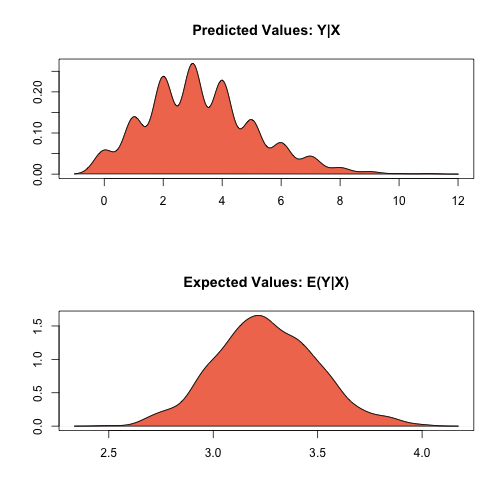
\includegraphics{Zelig-poisson-1.png}
\caption{Zelig-poisson}\end{figure}


\paragraph{Model}
\label{zelig-poisson:model}
Let \(Y_i\) be the number of independent events that occur during a
fixed time period. This variable can take any non-negative integer.
\begin{itemize}
\item {} 
The Poisson distribution has \emph{stochastic component}
\begin{gather}
\begin{split}Y_i \; \sim \; \textrm{Poisson}(\lambda_i),\end{split}\notag
\end{gather}
where \(\lambda_i\) is the mean and variance parameter.

\item {} 
The \emph{systematic component} is
\begin{gather}
\begin{split}\lambda_i \; = \; \exp(x_i \beta),\end{split}\notag
\end{gather}
where \(x_i\) is the vector of explanatory variables, and
\(\beta\) is the vector of coefficients.

\end{itemize}


\paragraph{Quantities of Interest}
\label{zelig-poisson:quantities-of-interest}\begin{itemize}
\item {} 
The expected value (qi\$ev) is the mean of simulations from the
stochastic component,
\begin{gather}
\begin{split}E(Y) = \lambda_i =  \exp(x_i
  \beta),\end{split}\notag
\end{gather}
given draws of \(\beta\) from its sampling distribution.

\item {} 
The predicted value (qi\$pr) is a random draw from the poisson
distribution defined by mean \(\lambda_i\).

\item {} 
The first difference in the expected values (qi\$fd) is given by:
\begin{gather}
\begin{split}\textrm{FD} \; = \; E(Y | x_1) - E(Y \mid x)\end{split}\notag
\end{gather}
\item {} 
In conditional prediction models, the average expected treatment
effect (att.ev) for the treatment group is
\begin{gather}
\begin{split}\frac{1}{\sum_{i=1}^n t_i}\sum_{i:t_i=1}^n \left\{ Y_i(t_i=1) -
      E[Y_i(t_i=0)] \right\},\end{split}\notag
\end{gather}
where \(t_i\) is a binary explanatory variable defining the
treatment (\(t_i=1\)) and control (\(t_i=0\)) groups.
Variation in the simulations are due to uncertainty in simulating
\(E[Y_i(t_i=0)]\), the counterfactual expected value of
\(Y_i\) for observations in the treatment group, under the
assumption that everything stays the same except that the treatment
indicator is switched to \(t_i=0\).

\item {} 
In conditional prediction models, the average predicted treatment
effect (att.pr) for the treatment group is
\begin{gather}
\begin{split}\frac{1}{\sum_{i=1}^n t_i}\sum_{i:t_i=1}^n \left\{ Y_i(t_i=1) -
      \widehat{Y_i(t_i=0)} \right\},\end{split}\notag
\end{gather}
where \(t_i\) is a binary explanatory variable defining the
treatment (\(t_i=1\)) and control (\(t_i=0\)) groups.
Variation in the simulations are due to uncertainty in simulating
\(\widehat{Y_i(t_i=0)}\), the counterfactual predicted value of
\(Y_i\) for observations in the treatment group, under the
assumption that everything stays the same except that the treatment
indicator is switched to \(t_i=0\).

\end{itemize}


\paragraph{Output Values}
\label{zelig-poisson:output-values}
The output of each Zelig command contains useful information which you
may view. For example, if you run
\code{z.out \textless{}- zelig(y \textasciitilde{} x, model = poisson, data)}, then you may examine
the available information in \code{z.out} by using \code{names(z.out)}, see
the coefficients by using z.out\$coefficients, and a default summary of
information through \code{summary(z.out)}.


\paragraph{See also}
\label{zelig-poisson:see-also}
The poisson model is part of the stats package by . Advanced users may
wish to refer to \code{help(glm)} and \code{help(family)}.


\subsubsection{zelig-probit}
\label{zelig-probit:zelig-probit}\label{zelig-probit::doc}\label{zelig-probit:zprobit}
Probit Regression for Dichotomous Dependent Variables

Use probit regression to model binary dependent variables specified as a
function of a set of explanatory variables.


\paragraph{Syntax}
\label{zelig-probit:syntax}
With reference classes:

\begin{Verbatim}[commandchars=\\\{\}]
z5 \PYG{o}{\PYGZlt{}\PYGZhy{}} zprobit\PYG{o}{\PYGZdl{}}new\PYG{p}{(}\PYG{p}{)}
z5\PYG{o}{\PYGZdl{}}zelig\PYG{p}{(}Y \PYG{o}{\PYGZti{}} X1 \PYG{o}{+} X \PYG{o}{\PYGZti{}} X\PYG{p}{,} data \PYG{o}{=} mydata\PYG{p}{)}
z5\PYG{o}{\PYGZdl{}}setx\PYG{p}{(}\PYG{p}{)}
z5\PYG{o}{\PYGZdl{}}sim\PYG{p}{(}\PYG{p}{)}
\end{Verbatim}

With the Zelig 4 compatibility wrappers:

\begin{Verbatim}[commandchars=\\\{\}]
z.out \PYG{o}{\PYGZlt{}\PYGZhy{}} zelig\PYG{p}{(}Y \PYG{o}{\PYGZti{}} X1 \PYG{o}{+} X2\PYG{p}{,} model \PYG{o}{=} \PYG{l+s}{\PYGZdq{}}\PYG{l+s}{probit\PYGZdq{}}\PYG{p}{,} data \PYG{o}{=} mydata\PYG{p}{)}
x.out \PYG{o}{\PYGZlt{}\PYGZhy{}} setx\PYG{p}{(}z.out\PYG{p}{)}
s.out \PYG{o}{\PYGZlt{}\PYGZhy{}} sim\PYG{p}{(}z.out\PYG{p}{,} x \PYG{o}{=} x.out\PYG{p}{,} x1 \PYG{o}{=} \PYG{k+kc}{NULL}\PYG{p}{)}
\end{Verbatim}


\paragraph{Example}
\label{zelig-probit:example}
Attach the sample turnout dataset:

\begin{Verbatim}[commandchars=\\\{\}]
data\PYG{p}{(}turnout\PYG{p}{)}
\end{Verbatim}

Estimate parameter values for the probit regression:

\begin{Verbatim}[commandchars=\\\{\}]
z.out \PYG{o}{\PYGZlt{}\PYGZhy{}} zelig\PYG{p}{(}vote \PYG{o}{\PYGZti{}} race \PYG{o}{+} educate\PYG{p}{,} model \PYG{o}{=} \PYG{l+s}{\PYGZdq{}}\PYG{l+s}{probit\PYGZdq{}}\PYG{p}{,} data \PYG{o}{=} turnout\PYG{p}{)}
\end{Verbatim}

\begin{Verbatim}[commandchars=\\\{\}]
\PYG{c}{\PYGZsh{}\PYGZsh{} How to cite this model in Zelig:}
\PYG{c}{\PYGZsh{}\PYGZsh{}   Kosuke Imai, Gary King, Olivia Lau. 2007.}
\PYG{c}{\PYGZsh{}\PYGZsh{}   probit: Probit Regression for Dichotomous Dependent Variables}
\PYG{c}{\PYGZsh{}\PYGZsh{}   in Kosuke Imai, Gary King, and Olivia Lau, \PYGZdq{}Zelig: Everyone\PYGZsq{}s Statistical Software,\PYGZdq{}}
\PYG{c}{\PYGZsh{}\PYGZsh{}   http://zeligproject.org/}
\end{Verbatim}

\begin{Verbatim}[commandchars=\\\{\}]
summary\PYG{p}{(}z.out\PYG{p}{)}
\end{Verbatim}

\begin{Verbatim}[commandchars=\\\{\}]
\PYG{c}{\PYGZsh{}\PYGZsh{} Model:}
\PYG{c}{\PYGZsh{}\PYGZsh{} \PYGZdl{}by}
\PYG{c}{\PYGZsh{}\PYGZsh{} [1] 1}
\PYG{c}{\PYGZsh{}\PYGZsh{}}
\PYG{c}{\PYGZsh{}\PYGZsh{}}
\PYG{c}{\PYGZsh{}\PYGZsh{} Call:  stats::glm(formula = vote \PYGZti{} race + educate, family = binomial(\PYGZdq{}probit\PYGZdq{}),}
\PYG{c}{\PYGZsh{}\PYGZsh{}     data = .)}
\PYG{c}{\PYGZsh{}\PYGZsh{}}
\PYG{c}{\PYGZsh{}\PYGZsh{} Coefficients:}
\PYG{c}{\PYGZsh{}\PYGZsh{} (Intercept)    racewhite      educate}
\PYG{c}{\PYGZsh{}\PYGZsh{}    \PYGZhy{}0.72595      0.29908      0.09712}
\PYG{c}{\PYGZsh{}\PYGZsh{}}
\PYG{c}{\PYGZsh{}\PYGZsh{} Degrees of Freedom: 1999 Total (i.e. Null);  1997 Residual}
\PYG{c}{\PYGZsh{}\PYGZsh{} Null Deviance:       2267}
\PYG{c}{\PYGZsh{}\PYGZsh{} Residual Deviance: 2136  AIC: 2142}
\PYG{c}{\PYGZsh{}\PYGZsh{} Next step: Use \PYGZsq{}setx\PYGZsq{} method}
\end{Verbatim}

Set values for the explanatory variables to their default values.

\begin{Verbatim}[commandchars=\\\{\}]
x.out \PYG{o}{\PYGZlt{}\PYGZhy{}} setx\PYG{p}{(}z.out\PYG{p}{)}
\end{Verbatim}

Simulate quantities of interest from the posterior distribution.

\begin{Verbatim}[commandchars=\\\{\}]
s.out \PYG{o}{\PYGZlt{}\PYGZhy{}} sim\PYG{p}{(}z.out\PYG{p}{,} x \PYG{o}{=} x.out\PYG{p}{)}
\end{Verbatim}

\begin{Verbatim}[commandchars=\\\{\}]
summary\PYG{p}{(}s.out\PYG{p}{)}
\end{Verbatim}

\begin{Verbatim}[commandchars=\\\{\}]
plot\PYG{p}{(}s.out1\PYG{p}{)}
\end{Verbatim}
\begin{figure}[htbp]
\centering
\capstart

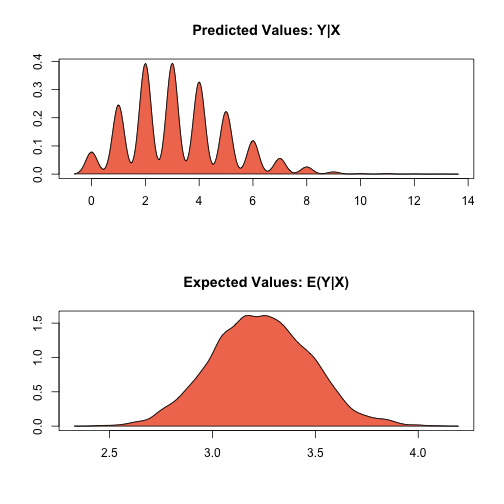
\includegraphics{Zelig-probit-1.png}
\caption{Zelig-probit}\end{figure}


\paragraph{Model}
\label{zelig-probit:model}
Let \(Y_i\) be the observed binary dependent variable for
observation \(i\) which takes the value of either 0 or 1.
\begin{itemize}
\item {} 
The \emph{stochastic component} is given by
\begin{gather}
\begin{split}Y_i \; \sim \; \textrm{Bernoulli}(\pi_i),\end{split}\notag
\end{gather}
where \(\pi_i=\Pr(Y_i=1)\).

\item {} 
The \emph{systematic component} is
\begin{gather}
\begin{split}\pi_i \; = \; \Phi (x_i \beta)\end{split}\notag
\end{gather}
where \(\Phi(\mu)\) is the cumulative distribution function of
the Normal distribution with mean 0 and unit variance.

\end{itemize}


\paragraph{Quantities of Interest}
\label{zelig-probit:quantities-of-interest}\begin{itemize}
\item {} 
The expected value (qi\$ev) is a simulation of predicted probability
of success
\begin{gather}
\begin{split}E(Y) = \pi_i = \Phi(x_i
  \beta),\end{split}\notag
\end{gather}
given a draw of \(\beta\) from its sampling distribution.

\item {} 
The predicted value (qi\$pr) is a draw from a Bernoulli distribution
with mean \(\pi_i\).

\item {} 
The first difference (qi\$fd) in expected values is defined as
\begin{gather}
\begin{split}\textrm{FD} = \Pr(Y = 1 \mid x_1) - \Pr(Y = 1 \mid x).\end{split}\notag
\end{gather}
\item {} 
The risk ratio (qi\$rr) is defined as
\begin{gather}
\begin{split}\textrm{RR} = \Pr(Y = 1 \mid x_1) / \Pr(Y = 1 \mid x).\end{split}\notag
\end{gather}
\item {} 
In conditional prediction models, the average expected treatment
effect (att.ev) for the treatment group is
\begin{gather}
\begin{split}\frac{1}{\sum_{i=1}^n t_i}\sum_{i:t_i=1}^n \left\{ Y_i(t_i=1) -
      E[Y_i(t_i=0)] \right\},\end{split}\notag
\end{gather}
where \(t_i\) is a binary explanatory variable defining the
treatment (\(t_i=1\)) and control (\(t_i=0\)) groups.
Variation in the simulations are due to uncertainty in simulating
\(E[Y_i(t_i=0)]\), the counterfactual expected value of
\(Y_i\) for observations in the treatment group, under the
assumption that everything stays the same except that the treatment
indicator is switched to \(t_i=0\).

\item {} 
In conditional prediction models, the average predicted treatment
effect (att.pr) for the treatment group is
\begin{gather}
\begin{split}\frac{1}{\sum_{i=1}^n t_i}\sum_{i:t_i=1}^n \left\{ Y_i(t_i=1) -
      \widehat{Y_i(t_i=0)} \right\},\end{split}\notag
\end{gather}
where \(t_i\) is a binary explanatory variable defining the
treatment (\(t_i=1\)) and control (\(t_i=0\)) groups.
Variation in the simulations are due to uncertainty in simulating
\(\widehat{Y_i(t_i=0)}\), the counterfactual predicted value of
\(Y_i\) for observations in the treatment group, under the
assumption that everything stays the same except that the treatment
indicator is switched to \(t_i=0\).

\end{itemize}


\paragraph{Output Values}
\label{zelig-probit:output-values}
The output of each Zelig command contains useful information which you
may view. For example, if you run
\code{z.out \textless{}- zelig(y \textasciitilde{} x, model = probit, data)}, then you may examine
the available information in \code{z.out} by using \code{names(z.out)}, see
the coefficients by using z.out\$coefficients, and a default summary of
information through \code{summary(z.out)}.


\paragraph{See also}
\label{zelig-probit:see-also}
The probit model is part of the stats package by . Advanced users may
wish to refer to \code{help(glm)} and \code{help(family)}.


\subsubsection{zelig-relogit}
\label{zelig-relogit:zrelogit}\label{zelig-relogit::doc}\label{zelig-relogit:zelig-relogit}
Rare Events Logistic Regression for Dichotomous Dependent Variables

The relogit procedure estimates the same model as standard logistic
regression (appropriate when you have a dichotomous dependent variable
and a set of explanatory variables; see ), but the estimates are
corrected for the bias that occurs when the sample is small or the
observed events are rare (i.e., if the dependent variable has many more
1s than 0s or the reverse). The relogit procedure also optionally uses
prior correction for case-control sampling designs.


\paragraph{Syntax}
\label{zelig-relogit:syntax}
With reference classes:

\begin{Verbatim}[commandchars=\\\{\}]
z5 \PYG{o}{\PYGZlt{}\PYGZhy{}} zrelogit\PYG{o}{\PYGZdl{}}new\PYG{p}{(}\PYG{p}{)}
z5\PYG{o}{\PYGZdl{}}zelig\PYG{p}{(}Y \PYG{o}{\PYGZti{}} X1 \PYG{o}{+} X2\PYG{p}{,} tau \PYG{o}{=} \PYG{k+kc}{NULL}\PYG{p}{,}
                       case.control \PYG{o}{=} c\PYG{p}{(}\PYG{l+s}{\PYGZdq{}}\PYG{l+s}{prior\PYGZdq{}}\PYG{p}{,} \PYG{l+s}{\PYGZdq{}}\PYG{l+s}{weighting\PYGZdq{}}\PYG{p}{)}\PYG{p}{,}
                       bias.correct \PYG{o}{=} \PYG{k+kc}{TRUE}\PYG{p}{,} robust \PYG{o}{=} \PYG{k+kc}{FALSE}\PYG{p}{,}
                       data \PYG{o}{=} mydata\PYG{p}{,} \PYG{k+kc}{...}\PYG{p}{)}
z5\PYG{o}{\PYGZdl{}}setx\PYG{p}{(}\PYG{p}{)}
z5\PYG{o}{\PYGZdl{}}sim\PYG{p}{(}\PYG{p}{)}
\end{Verbatim}

With the Zelig 4 compatibility wrappers:

\begin{Verbatim}[commandchars=\\\{\}]
z.out \PYG{o}{\PYGZlt{}\PYGZhy{}} zelig\PYG{p}{(}Y \PYG{o}{\PYGZti{}} X1 \PYG{o}{+} X2\PYG{p}{,} model \PYG{o}{=} \PYG{l+s}{\PYGZdq{}}\PYG{l+s}{relogit\PYGZdq{}}\PYG{p}{,} tau \PYG{o}{=} \PYG{k+kc}{NULL}\PYG{p}{,}
                       case.control \PYG{o}{=} c\PYG{p}{(}\PYG{l+s}{\PYGZdq{}}\PYG{l+s}{prior\PYGZdq{}}\PYG{p}{,} \PYG{l+s}{\PYGZdq{}}\PYG{l+s}{weighting\PYGZdq{}}\PYG{p}{)}\PYG{p}{,}
                       bias.correct \PYG{o}{=} \PYG{k+kc}{TRUE}\PYG{p}{,} robust \PYG{o}{=} \PYG{k+kc}{FALSE}\PYG{p}{,}
                       data \PYG{o}{=} mydata\PYG{p}{,} \PYG{k+kc}{...}\PYG{p}{)}
x.out \PYG{o}{\PYGZlt{}\PYGZhy{}} setx\PYG{p}{(}z.out\PYG{p}{)}
s.out \PYG{o}{\PYGZlt{}\PYGZhy{}} sim\PYG{p}{(}z.out\PYG{p}{,} x \PYG{o}{=} x.out\PYG{p}{)}
\end{Verbatim}


\paragraph{Arguments}
\label{zelig-relogit:arguments}
The relogit procedure supports four optional arguments in addition to
the standard arguments for zelig(). You may additionally use:
\begin{itemize}
\item {} 
tau: a vector containing either one or two values for \(\tau\),
the true population fraction of ones. Use, for example, tau = c(0.05,
0.1) to specify that the lower bound on tau is 0.05 and the upper
bound is 0.1. If left unspecified, only finite-sample bias correction
is performed, not case-control correction.

\item {} 
case.control: if tau is specified, choose a method to correct for
case-control sampling design: “prior” (default) or “weighting”.

\item {} 
bias.correct: a logical value of TRUE (default) or FALSE indicating
whether the intercept should be corrected for finite sample (rare
events) bias.

\end{itemize}

Note that if tau = NULL, bias.correct = FALSE, the
relogit procedure performs a standard logistic regression without any
correction.


\paragraph{Example 1: One Tau with Prior Correction and Bias Correction}
\label{zelig-relogit:example-1-one-tau-with-prior-correction-and-bias-correction}
Due to memory and space considerations, the data used here are a sample
drawn from the full data set used in King and Zeng, 2001, The proportion
of militarized interstate conflicts to the absence of disputes is
\(\tau = 1,042 / 303,772
\approx 0.00343\). To estimate the model,

\begin{Verbatim}[commandchars=\\\{\}]
data\PYG{p}{(}mid\PYG{p}{)}
\end{Verbatim}

\begin{Verbatim}[commandchars=\\\{\}]
z.out1 \PYG{o}{\PYGZlt{}\PYGZhy{}} zelig\PYG{p}{(}conflict \PYG{o}{\PYGZti{}} major \PYG{o}{+} contig \PYG{o}{+} power \PYG{o}{+} maxdem \PYG{o}{+} mindem \PYG{o}{+} years\PYG{p}{,} data \PYG{o}{=} mid\PYG{p}{,} model \PYG{o}{=} \PYG{l+s}{\PYGZdq{}}\PYG{l+s}{relogit\PYGZdq{}}\PYG{p}{,} tau \PYG{o}{=} \PYG{l+m}{1042}\PYG{o}{/}\PYG{l+m}{303772}\PYG{p}{)}
\end{Verbatim}

\begin{Verbatim}[commandchars=\\\{\}]
\PYG{c}{\PYGZsh{}\PYGZsh{} How to cite this model in Zelig:}
\PYG{c}{\PYGZsh{}\PYGZsh{}   Kosuke Imai, Gary King, and Olivia Lau. 2014.}
\PYG{c}{\PYGZsh{}\PYGZsh{}   relogit: Rare Events Logistic Regression for Dichotomous Dependent Variables}
\PYG{c}{\PYGZsh{}\PYGZsh{}   in Kosuke Imai, Gary King, and Olivia Lau, \PYGZdq{}Zelig: Everyone\PYGZsq{}s Statistical Software,\PYGZdq{}}
\PYG{c}{\PYGZsh{}\PYGZsh{}   http://zeligproject.org/}
\end{Verbatim}

Summarize the model output:

\begin{Verbatim}[commandchars=\\\{\}]
summary\PYG{p}{(}z.out1\PYG{p}{)}
\end{Verbatim}

\begin{Verbatim}[commandchars=\\\{\}]
\PYG{c}{\PYGZsh{}\PYGZsh{} Model:}
\PYG{c}{\PYGZsh{}\PYGZsh{} \PYGZdl{}by}
\PYG{c}{\PYGZsh{}\PYGZsh{} [1] 1}
\PYG{c}{\PYGZsh{}\PYGZsh{}}
\PYG{c}{\PYGZsh{}\PYGZsh{}}
\PYG{c}{\PYGZsh{}\PYGZsh{} Call:  relogit(formula = cbind(conflict, 1 \PYGZhy{} conflict) \PYGZti{} major + contig +}
\PYG{c}{\PYGZsh{}\PYGZsh{}     power + maxdem + mindem + years, data = ., tau = 0.00343020423212146,}
\PYG{c}{\PYGZsh{}\PYGZsh{}     bias.correct = TRUE, case.control = \PYGZdq{}prior\PYGZdq{})}
\PYG{c}{\PYGZsh{}\PYGZsh{}}
\PYG{c}{\PYGZsh{}\PYGZsh{} Coefficients:}
\PYG{c}{\PYGZsh{}\PYGZsh{} (Intercept)        major       contig        power       maxdem}
\PYG{c}{\PYGZsh{}\PYGZsh{}    \PYGZhy{}7.50836      2.43196      4.10797      1.05358      0.04804}
\PYG{c}{\PYGZsh{}\PYGZsh{}      mindem        years}
\PYG{c}{\PYGZsh{}\PYGZsh{}    \PYGZhy{}0.06413     \PYGZhy{}0.06293}
\PYG{c}{\PYGZsh{}\PYGZsh{}}
\PYG{c}{\PYGZsh{}\PYGZsh{} Degrees of Freedom: 3125 Total (i.e. Null);  3119 Residual}
\PYG{c}{\PYGZsh{}\PYGZsh{} Null Deviance:       3979}
\PYG{c}{\PYGZsh{}\PYGZsh{} Residual Deviance: 1869  AIC: 1883}
\PYG{c}{\PYGZsh{}\PYGZsh{} Next step: Use \PYGZsq{}setx\PYGZsq{} method}
\end{Verbatim}

Set the explanatory variables to their means:

\begin{Verbatim}[commandchars=\\\{\}]
x.out1 \PYG{o}{\PYGZlt{}\PYGZhy{}} setx\PYG{p}{(}z.out1\PYG{p}{)}
\end{Verbatim}

Simulate quantities of interest:

\begin{Verbatim}[commandchars=\\\{\}]
s.out1 \PYG{o}{\PYGZlt{}\PYGZhy{}} sim\PYG{p}{(}z.out1\PYG{p}{,} x \PYG{o}{=} x.out1\PYG{p}{)}
summary\PYG{p}{(}s.out1\PYG{p}{)}
\end{Verbatim}

\begin{Verbatim}[commandchars=\\\{\}]
\PYG{c}{\PYGZsh{}\PYGZsh{}}
\PYG{c}{\PYGZsh{}\PYGZsh{}  sim x :}
\PYG{c}{\PYGZsh{}\PYGZsh{}  \PYGZhy{}\PYGZhy{}\PYGZhy{}\PYGZhy{}\PYGZhy{}}
\PYG{c}{\PYGZsh{}\PYGZsh{} ev}
\PYG{c}{\PYGZsh{}\PYGZsh{}             mean          sd         50\PYGZpc{}        2.5\PYGZpc{}       97.5\PYGZpc{}}
\PYG{c}{\PYGZsh{}\PYGZsh{} [1,] 0.002402049 0.000157269 0.002399256 0.002087972 0.002716099}
\PYG{c}{\PYGZsh{}\PYGZsh{} pv}
\PYG{c}{\PYGZsh{}\PYGZsh{}          0     1}
\PYG{c}{\PYGZsh{}\PYGZsh{} [1,] 0.997 0.003}
\end{Verbatim}

\begin{Verbatim}[commandchars=\\\{\}]
plot\PYG{p}{(}s.out1\PYG{p}{)}
\end{Verbatim}
\begin{figure}[htbp]
\centering
\capstart


\includegraphics{Zelig-relogit-1.png}
\caption{Zelig-relogit}\end{figure}


\paragraph{Example 2: One Tau with Weighting, Robust Standard Errors, and Bias Correction}
\label{zelig-relogit:example-2-one-tau-with-weighting-robust-standard-errors-and-bias-correction}
Suppose that we wish to perform case control correction using weighting
(rather than the default prior correction). To estimate the model:

\begin{Verbatim}[commandchars=\\\{\}]
z.out2 \PYG{o}{\PYGZlt{}\PYGZhy{}} zelig\PYG{p}{(}conflict \PYG{o}{\PYGZti{}} major \PYG{o}{+} contig \PYG{o}{+} power \PYG{o}{+} maxdem \PYG{o}{+} mindem \PYG{o}{+} years\PYG{p}{,} data \PYG{o}{=} mid\PYG{p}{,} model \PYG{o}{=} \PYG{l+s}{\PYGZdq{}}\PYG{l+s}{relogit\PYGZdq{}}\PYG{p}{,} tau \PYG{o}{=} \PYG{l+m}{1042}\PYG{o}{/}\PYG{l+m}{303772}\PYG{p}{,} case.control \PYG{o}{=} \PYG{l+s}{\PYGZdq{}}\PYG{l+s}{weighting\PYGZdq{}}\PYG{p}{,} robust \PYG{o}{=} \PYG{k+kc}{TRUE}\PYG{p}{)}
\end{Verbatim}

\begin{Verbatim}[commandchars=\\\{\}]
\PYG{c}{\PYGZsh{}\PYGZsh{} Error in glm.control(robust = TRUE): unused argument (robust = TRUE)}
\end{Verbatim}

Summarize the model output:

\begin{Verbatim}[commandchars=\\\{\}]
summary\PYG{p}{(}z.out2\PYG{p}{)}
\end{Verbatim}

\begin{Verbatim}[commandchars=\\\{\}]
\PYG{c}{\PYGZsh{}\PYGZsh{} Model:}
\PYG{c}{\PYGZsh{}\PYGZsh{} \PYGZdl{}by}
\PYG{c}{\PYGZsh{}\PYGZsh{} [1] 1}
\PYG{c}{\PYGZsh{}\PYGZsh{}}
\PYG{c}{\PYGZsh{}\PYGZsh{}}
\PYG{c}{\PYGZsh{}\PYGZsh{} Call:  stats::glm(formula = vote \PYGZti{} race + educate, family = binomial(\PYGZdq{}logit\PYGZdq{}),}
\PYG{c}{\PYGZsh{}\PYGZsh{}     data = .)}
\PYG{c}{\PYGZsh{}\PYGZsh{}}
\PYG{c}{\PYGZsh{}\PYGZsh{} Coefficients:}
\PYG{c}{\PYGZsh{}\PYGZsh{} (Intercept)    racewhite      educate}
\PYG{c}{\PYGZsh{}\PYGZsh{}     \PYGZhy{}1.2189       0.5022       0.1610}
\PYG{c}{\PYGZsh{}\PYGZsh{}}
\PYG{c}{\PYGZsh{}\PYGZsh{} Degrees of Freedom: 1999 Total (i.e. Null);  1997 Residual}
\PYG{c}{\PYGZsh{}\PYGZsh{} Null Deviance:       2267}
\PYG{c}{\PYGZsh{}\PYGZsh{} Residual Deviance: 2138  AIC: 2144}
\PYG{c}{\PYGZsh{}\PYGZsh{} Next step: Use \PYGZsq{}setx\PYGZsq{} method}
\end{Verbatim}

Set the explanatory variables to their means:

\begin{Verbatim}[commandchars=\\\{\}]
x.out2 \PYG{o}{\PYGZlt{}\PYGZhy{}} setx\PYG{p}{(}z.out2\PYG{p}{)}
\end{Verbatim}

Simulate quantities of interest:

\begin{Verbatim}[commandchars=\\\{\}]
s.out2 \PYG{o}{\PYGZlt{}\PYGZhy{}} sim\PYG{p}{(}z.out2\PYG{p}{,} x \PYG{o}{=} x.out2\PYG{p}{)}
summary\PYG{p}{(}s.out2\PYG{p}{)}
\end{Verbatim}

\begin{Verbatim}[commandchars=\\\{\}]
\PYG{c}{\PYGZsh{}\PYGZsh{}}
\PYG{c}{\PYGZsh{}\PYGZsh{}  sim x :}
\PYG{c}{\PYGZsh{}\PYGZsh{}  \PYGZhy{}\PYGZhy{}\PYGZhy{}\PYGZhy{}\PYGZhy{}}
\PYG{c}{\PYGZsh{}\PYGZsh{} ev}
\PYG{c}{\PYGZsh{}\PYGZsh{}           mean         sd      50\PYGZpc{}      2.5\PYGZpc{}     97.5\PYGZpc{}}
\PYG{c}{\PYGZsh{}\PYGZsh{} [1,] 0.7724619 0.01000481 0.772542 0.7532891 0.7918851}
\PYG{c}{\PYGZsh{}\PYGZsh{} pv}
\PYG{c}{\PYGZsh{}\PYGZsh{}          0     1}
\PYG{c}{\PYGZsh{}\PYGZsh{} [1,] 0.202 0.798}
\end{Verbatim}


\paragraph{Example 3: Two Taus with Bias Correction and Prior Correction}
\label{zelig-relogit:example-3-two-taus-with-bias-correction-and-prior-correction}
Suppose that we did not know that \(\tau \approx 0.00343\), but only
that it was somewhere between \((0.002, 0.005)\). To estimate a
model with a range of feasible estimates for \(\tau\) (using the
default prior correction method for case control correction):

\begin{Verbatim}[commandchars=\\\{\}]
z.out2 \PYG{o}{\PYGZlt{}\PYGZhy{}} zelig\PYG{p}{(}conflict \PYG{o}{\PYGZti{}} major \PYG{o}{+} contig \PYG{o}{+} power \PYG{o}{+} maxdem \PYG{o}{+} mindem \PYG{o}{+} years\PYG{p}{,} data \PYG{o}{=} mid\PYG{p}{,} model \PYG{o}{=} \PYG{l+s}{\PYGZdq{}}\PYG{l+s}{relogit\PYGZdq{}}\PYG{p}{,} tau \PYG{o}{=} c\PYG{p}{(}\PYG{l+m}{0.002}\PYG{p}{,} \PYG{l+m}{0.005}\PYG{p}{)}\PYG{p}{)}
\end{Verbatim}

\begin{Verbatim}[commandchars=\\\{\}]
\PYG{c}{\PYGZsh{}\PYGZsh{} How to cite this model in Zelig:}
\PYG{c}{\PYGZsh{}\PYGZsh{}   Kosuke Imai, Gary King, and Olivia Lau. 2014.}
\PYG{c}{\PYGZsh{}\PYGZsh{}   relogit: Rare Events Logistic Regression for Dichotomous Dependent Variables}
\PYG{c}{\PYGZsh{}\PYGZsh{}   in Kosuke Imai, Gary King, and Olivia Lau, \PYGZdq{}Zelig: Everyone\PYGZsq{}s Statistical Software,\PYGZdq{}}
\PYG{c}{\PYGZsh{}\PYGZsh{}   http://zeligproject.org/}
\end{Verbatim}

Summarize the model output:

\begin{Verbatim}[commandchars=\\\{\}]
z.out2
\end{Verbatim}

\begin{Verbatim}[commandchars=\\\{\}]
\PYG{c}{\PYGZsh{}\PYGZsh{} Model:}
\PYG{c}{\PYGZsh{}\PYGZsh{} \PYGZdl{}by}
\PYG{c}{\PYGZsh{}\PYGZsh{} [1] 1}
\PYG{c}{\PYGZsh{}\PYGZsh{}}
\PYG{c}{\PYGZsh{}\PYGZsh{} \PYGZdl{}lower.estimate}
\PYG{c}{\PYGZsh{}\PYGZsh{}}
\PYG{c}{\PYGZsh{}\PYGZsh{} Call:  (function (formula, data = sys.parent(), tau = NULL, bias.correct = TRUE,}
\PYG{c}{\PYGZsh{}\PYGZsh{}     case.control = \PYGZdq{}prior\PYGZdq{}, ...)}
\PYG{c}{\PYGZsh{}\PYGZsh{} \PYGZob{}}
\PYG{c}{\PYGZsh{}\PYGZsh{}     mf \PYGZlt{}\PYGZhy{} match.call()}
\PYG{c}{\PYGZsh{}\PYGZsh{}     mf\PYGZdl{}tau \PYGZlt{}\PYGZhy{} mf\PYGZdl{}bias.correct \PYGZlt{}\PYGZhy{} mf\PYGZdl{}case.control \PYGZlt{}\PYGZhy{} NULL}
\PYG{c}{\PYGZsh{}\PYGZsh{}     if (!is.null(tau)) \PYGZob{}}
\PYG{c}{\PYGZsh{}\PYGZsh{}         tau \PYGZlt{}\PYGZhy{} unique(tau)}
\PYG{c}{\PYGZsh{}\PYGZsh{}         if (length(case.control) \PYGZgt{} 1)}
\PYG{c}{\PYGZsh{}\PYGZsh{}             stop(\PYGZdq{}You can only choose one option for case control correction.\PYGZdq{})}
\PYG{c}{\PYGZsh{}\PYGZsh{}         ck1 \PYGZlt{}\PYGZhy{} grep(\PYGZdq{}p\PYGZdq{}, case.control)}
\PYG{c}{\PYGZsh{}\PYGZsh{}         ck2 \PYGZlt{}\PYGZhy{} grep(\PYGZdq{}w\PYGZdq{}, case.control)}
\PYG{c}{\PYGZsh{}\PYGZsh{}         if (length(ck1) == 0 \PYGZam{} length(ck2) == 0)}
\PYG{c}{\PYGZsh{}\PYGZsh{}             stop(\PYGZdq{}choose either case.control = \PYGZbs{}\PYGZdq{}prior\PYGZbs{}\PYGZdq{} \PYGZdq{}, \PYGZdq{}or case.control = \PYGZbs{}\PYGZdq{}weighting\PYGZbs{}\PYGZdq{}\PYGZdq{})}
\PYG{c}{\PYGZsh{}\PYGZsh{}         if (length(ck2) == 0)}
\PYG{c}{\PYGZsh{}\PYGZsh{}             weighting \PYGZlt{}\PYGZhy{} FALSE}
\PYG{c}{\PYGZsh{}\PYGZsh{}         else weighting \PYGZlt{}\PYGZhy{} TRUE}
\PYG{c}{\PYGZsh{}\PYGZsh{}     \PYGZcb{}}
\PYG{c}{\PYGZsh{}\PYGZsh{}     else weighting \PYGZlt{}\PYGZhy{} FALSE}
\PYG{c}{\PYGZsh{}\PYGZsh{}     if (length(tau) \PYGZgt{} 2)}
\PYG{c}{\PYGZsh{}\PYGZsh{}         stop(\PYGZdq{}tau must be a vector of length less than or equal to 2\PYGZdq{})}
\PYG{c}{\PYGZsh{}\PYGZsh{}     else if (length(tau) == 2) \PYGZob{}}
\PYG{c}{\PYGZsh{}\PYGZsh{}         mf[[1]] \PYGZlt{}\PYGZhy{} relogit}
\PYG{c}{\PYGZsh{}\PYGZsh{}         res \PYGZlt{}\PYGZhy{} list()}
\PYG{c}{\PYGZsh{}\PYGZsh{}         mf\PYGZdl{}tau \PYGZlt{}\PYGZhy{} min(tau)}
\PYG{c}{\PYGZsh{}\PYGZsh{}         res\PYGZdl{}lower.estimate \PYGZlt{}\PYGZhy{} eval(as.call(mf), parent.frame())}
\PYG{c}{\PYGZsh{}\PYGZsh{}         mf\PYGZdl{}tau \PYGZlt{}\PYGZhy{} max(tau)}
\PYG{c}{\PYGZsh{}\PYGZsh{}         res\PYGZdl{}upper.estimate \PYGZlt{}\PYGZhy{} eval(as.call(mf), parent.frame())}
\PYG{c}{\PYGZsh{}\PYGZsh{}         res\PYGZdl{}formula \PYGZlt{}\PYGZhy{} formula}
\PYG{c}{\PYGZsh{}\PYGZsh{}         class(res) \PYGZlt{}\PYGZhy{} c(\PYGZdq{}Relogit2\PYGZdq{}, \PYGZdq{}Relogit\PYGZdq{})}
\PYG{c}{\PYGZsh{}\PYGZsh{}         return(res)}
\PYG{c}{\PYGZsh{}\PYGZsh{}     \PYGZcb{}}
\PYG{c}{\PYGZsh{}\PYGZsh{}     else \PYGZob{}}
\PYG{c}{\PYGZsh{}\PYGZsh{}         mf[[1]] \PYGZlt{}\PYGZhy{} glm}
\PYG{c}{\PYGZsh{}\PYGZsh{}         mf\PYGZdl{}family \PYGZlt{}\PYGZhy{} binomial(link = \PYGZdq{}logit\PYGZdq{})}
\PYG{c}{\PYGZsh{}\PYGZsh{}         y2 \PYGZlt{}\PYGZhy{} model.response(model.frame(mf\PYGZdl{}formula, data))}
\PYG{c}{\PYGZsh{}\PYGZsh{}         if (is.matrix(y2))}
\PYG{c}{\PYGZsh{}\PYGZsh{}             y \PYGZlt{}\PYGZhy{} y2[, 1]}
\PYG{c}{\PYGZsh{}\PYGZsh{}         else y \PYGZlt{}\PYGZhy{} y2}
\PYG{c}{\PYGZsh{}\PYGZsh{}         ybar \PYGZlt{}\PYGZhy{} mean(y)}
\PYG{c}{\PYGZsh{}\PYGZsh{}         if (weighting) \PYGZob{}}
\PYG{c}{\PYGZsh{}\PYGZsh{}             w1 \PYGZlt{}\PYGZhy{} tau/ybar}
\PYG{c}{\PYGZsh{}\PYGZsh{}             w0 \PYGZlt{}\PYGZhy{} (1 \PYGZhy{} tau)/(1 \PYGZhy{} ybar)}
\PYG{c}{\PYGZsh{}\PYGZsh{}             wi \PYGZlt{}\PYGZhy{} w1 * y + w0 * (1 \PYGZhy{} y)}
\PYG{c}{\PYGZsh{}\PYGZsh{}             mf\PYGZdl{}weights \PYGZlt{}\PYGZhy{} wi}
\PYG{c}{\PYGZsh{}\PYGZsh{}         \PYGZcb{}}
\PYG{c}{\PYGZsh{}\PYGZsh{}         res \PYGZlt{}\PYGZhy{} eval(as.call(mf), parent.frame())}
\PYG{c}{\PYGZsh{}\PYGZsh{}         res\PYGZdl{}call \PYGZlt{}\PYGZhy{} match.call(expand.dots = TRUE)}
\PYG{c}{\PYGZsh{}\PYGZsh{}         res\PYGZdl{}tau \PYGZlt{}\PYGZhy{} tau}
\PYG{c}{\PYGZsh{}\PYGZsh{}         X \PYGZlt{}\PYGZhy{} model.matrix(res)}
\PYG{c}{\PYGZsh{}\PYGZsh{}         if (bias.correct) \PYGZob{}}
\PYG{c}{\PYGZsh{}\PYGZsh{}             pihat \PYGZlt{}\PYGZhy{} fitted(res)}
\PYG{c}{\PYGZsh{}\PYGZsh{}             if (is.null(tau))}
\PYG{c}{\PYGZsh{}\PYGZsh{}                 wi \PYGZlt{}\PYGZhy{} rep(1, length(y))}
\PYG{c}{\PYGZsh{}\PYGZsh{}             else if (weighting)}
\PYG{c}{\PYGZsh{}\PYGZsh{}                 res\PYGZdl{}weighting \PYGZlt{}\PYGZhy{} TRUE}
\PYG{c}{\PYGZsh{}\PYGZsh{}             else \PYGZob{}}
\PYG{c}{\PYGZsh{}\PYGZsh{}                 w1 \PYGZlt{}\PYGZhy{} tau/ybar}
\PYG{c}{\PYGZsh{}\PYGZsh{}                 w0 \PYGZlt{}\PYGZhy{} (1 \PYGZhy{} tau)/(1 \PYGZhy{} ybar)}
\PYG{c}{\PYGZsh{}\PYGZsh{}                 wi \PYGZlt{}\PYGZhy{} w1 * y + w0 * (1 \PYGZhy{} y)}
\PYG{c}{\PYGZsh{}\PYGZsh{}                 res\PYGZdl{}weighting \PYGZlt{}\PYGZhy{} FALSE}
\PYG{c}{\PYGZsh{}\PYGZsh{}             \PYGZcb{}}
\PYG{c}{\PYGZsh{}\PYGZsh{}             W \PYGZlt{}\PYGZhy{} pihat * (1 \PYGZhy{} pihat) * wi}
\PYG{c}{\PYGZsh{}\PYGZsh{}             Qdiag \PYGZlt{}\PYGZhy{} lm.influence(lm(y \PYGZti{} X \PYGZhy{} 1, weights = W))\PYGZdl{}hat/W}
\PYG{c}{\PYGZsh{}\PYGZsh{}             if (is.null(tau))}
\PYG{c}{\PYGZsh{}\PYGZsh{}                 xi \PYGZlt{}\PYGZhy{} 0.5 * Qdiag * (2 * pihat \PYGZhy{} 1)}
\PYG{c}{\PYGZsh{}\PYGZsh{}             else xi \PYGZlt{}\PYGZhy{} 0.5 * Qdiag * ((1 + w0) * pihat \PYGZhy{} w0)}
\PYG{c}{\PYGZsh{}\PYGZsh{}             res\PYGZdl{}coefficients \PYGZlt{}\PYGZhy{} res\PYGZdl{}coefficients \PYGZhy{} lm(xi \PYGZti{} X \PYGZhy{}}
\PYG{c}{\PYGZsh{}\PYGZsh{}                 1, weights = W)\PYGZdl{}coefficients}
\PYG{c}{\PYGZsh{}\PYGZsh{}             res\PYGZdl{}bias.correct \PYGZlt{}\PYGZhy{} TRUE}
\PYG{c}{\PYGZsh{}\PYGZsh{}         \PYGZcb{}}
\PYG{c}{\PYGZsh{}\PYGZsh{}         else res\PYGZdl{}bias.correct \PYGZlt{}\PYGZhy{} FALSE}
\PYG{c}{\PYGZsh{}\PYGZsh{}         if (!is.null(tau) \PYGZam{} !weighting) \PYGZob{}}
\PYG{c}{\PYGZsh{}\PYGZsh{}             if (tau \PYGZlt{}= 0 \textbar{}\textbar{} tau \PYGZgt{}= 1)}
\PYG{c}{\PYGZsh{}\PYGZsh{}                 stop(\PYGZdq{}\PYGZbs{}ntau needs to be between 0 and 1.\PYGZbs{}n\PYGZdq{})}
\PYG{c}{\PYGZsh{}\PYGZsh{}             res\PYGZdl{}coefficients[\PYGZdq{}(Intercept)\PYGZdq{}] \PYGZlt{}\PYGZhy{} res\PYGZdl{}coefficients[\PYGZdq{}(Intercept)\PYGZdq{}] \PYGZhy{}}
\PYG{c}{\PYGZsh{}\PYGZsh{}                 log(((1 \PYGZhy{} tau)/tau) * (ybar/(1 \PYGZhy{} ybar)))}
\PYG{c}{\PYGZsh{}\PYGZsh{}             res\PYGZdl{}prior.correct \PYGZlt{}\PYGZhy{} TRUE}
\PYG{c}{\PYGZsh{}\PYGZsh{}             res\PYGZdl{}weighting \PYGZlt{}\PYGZhy{} FALSE}
\PYG{c}{\PYGZsh{}\PYGZsh{}         \PYGZcb{}}
\PYG{c}{\PYGZsh{}\PYGZsh{}         else res\PYGZdl{}prior.correct \PYGZlt{}\PYGZhy{} FALSE}
\PYG{c}{\PYGZsh{}\PYGZsh{}         if (is.null(res\PYGZdl{}weighting))}
\PYG{c}{\PYGZsh{}\PYGZsh{}             res\PYGZdl{}weighting \PYGZlt{}\PYGZhy{} FALSE}
\PYG{c}{\PYGZsh{}\PYGZsh{}         res\PYGZdl{}linear.predictors \PYGZlt{}\PYGZhy{} t(res\PYGZdl{}coefficients) \PYGZpc{}*\PYGZpc{} t(X)}
\PYG{c}{\PYGZsh{}\PYGZsh{}         res\PYGZdl{}fitted.values \PYGZlt{}\PYGZhy{} 1/(1 + exp(\PYGZhy{}res\PYGZdl{}linear.predictors))}
\PYG{c}{\PYGZsh{}\PYGZsh{}         res\PYGZdl{}zelig \PYGZlt{}\PYGZhy{} \PYGZdq{}Relogit\PYGZdq{}}
\PYG{c}{\PYGZsh{}\PYGZsh{}         class(res) \PYGZlt{}\PYGZhy{} c(\PYGZdq{}Relogit\PYGZdq{}, \PYGZdq{}glm\PYGZdq{})}
\PYG{c}{\PYGZsh{}\PYGZsh{}         return(res)}
\PYG{c}{\PYGZsh{}\PYGZsh{}     \PYGZcb{}}
\PYG{c}{\PYGZsh{}\PYGZsh{} \PYGZcb{})(formula = cbind(conflict, 1 \PYGZhy{} conflict) \PYGZti{} major + contig +}
\PYG{c}{\PYGZsh{}\PYGZsh{}     power + maxdem + mindem + years, data = ., tau = 0.002)}
\PYG{c}{\PYGZsh{}\PYGZsh{}}
\PYG{c}{\PYGZsh{}\PYGZsh{} Coefficients:}
\PYG{c}{\PYGZsh{}\PYGZsh{} (Intercept)        major       contig        power       maxdem}
\PYG{c}{\PYGZsh{}\PYGZsh{}    \PYGZhy{}8.04923      2.43196      4.10791      1.05357      0.04804}
\PYG{c}{\PYGZsh{}\PYGZsh{}      mindem        years}
\PYG{c}{\PYGZsh{}\PYGZsh{}    \PYGZhy{}0.06412     \PYGZhy{}0.06293}
\PYG{c}{\PYGZsh{}\PYGZsh{}}
\PYG{c}{\PYGZsh{}\PYGZsh{} Degrees of Freedom: 3125 Total (i.e. Null);  3119 Residual}
\PYG{c}{\PYGZsh{}\PYGZsh{} Null Deviance:       3979}
\PYG{c}{\PYGZsh{}\PYGZsh{} Residual Deviance: 1869  AIC: 1883}
\PYG{c}{\PYGZsh{}\PYGZsh{}}
\PYG{c}{\PYGZsh{}\PYGZsh{} \PYGZdl{}upper.estimate}
\PYG{c}{\PYGZsh{}\PYGZsh{}}
\PYG{c}{\PYGZsh{}\PYGZsh{} Call:  (function (formula, data = sys.parent(), tau = NULL, bias.correct = TRUE,}
\PYG{c}{\PYGZsh{}\PYGZsh{}     case.control = \PYGZdq{}prior\PYGZdq{}, ...)}
\PYG{c}{\PYGZsh{}\PYGZsh{} \PYGZob{}}
\PYG{c}{\PYGZsh{}\PYGZsh{}     mf \PYGZlt{}\PYGZhy{} match.call()}
\PYG{c}{\PYGZsh{}\PYGZsh{}     mf\PYGZdl{}tau \PYGZlt{}\PYGZhy{} mf\PYGZdl{}bias.correct \PYGZlt{}\PYGZhy{} mf\PYGZdl{}case.control \PYGZlt{}\PYGZhy{} NULL}
\PYG{c}{\PYGZsh{}\PYGZsh{}     if (!is.null(tau)) \PYGZob{}}
\PYG{c}{\PYGZsh{}\PYGZsh{}         tau \PYGZlt{}\PYGZhy{} unique(tau)}
\PYG{c}{\PYGZsh{}\PYGZsh{}         if (length(case.control) \PYGZgt{} 1)}
\PYG{c}{\PYGZsh{}\PYGZsh{}             stop(\PYGZdq{}You can only choose one option for case control correction.\PYGZdq{})}
\PYG{c}{\PYGZsh{}\PYGZsh{}         ck1 \PYGZlt{}\PYGZhy{} grep(\PYGZdq{}p\PYGZdq{}, case.control)}
\PYG{c}{\PYGZsh{}\PYGZsh{}         ck2 \PYGZlt{}\PYGZhy{} grep(\PYGZdq{}w\PYGZdq{}, case.control)}
\PYG{c}{\PYGZsh{}\PYGZsh{}         if (length(ck1) == 0 \PYGZam{} length(ck2) == 0)}
\PYG{c}{\PYGZsh{}\PYGZsh{}             stop(\PYGZdq{}choose either case.control = \PYGZbs{}\PYGZdq{}prior\PYGZbs{}\PYGZdq{} \PYGZdq{}, \PYGZdq{}or case.control = \PYGZbs{}\PYGZdq{}weighting\PYGZbs{}\PYGZdq{}\PYGZdq{})}
\PYG{c}{\PYGZsh{}\PYGZsh{}         if (length(ck2) == 0)}
\PYG{c}{\PYGZsh{}\PYGZsh{}             weighting \PYGZlt{}\PYGZhy{} FALSE}
\PYG{c}{\PYGZsh{}\PYGZsh{}         else weighting \PYGZlt{}\PYGZhy{} TRUE}
\PYG{c}{\PYGZsh{}\PYGZsh{}     \PYGZcb{}}
\PYG{c}{\PYGZsh{}\PYGZsh{}     else weighting \PYGZlt{}\PYGZhy{} FALSE}
\PYG{c}{\PYGZsh{}\PYGZsh{}     if (length(tau) \PYGZgt{} 2)}
\PYG{c}{\PYGZsh{}\PYGZsh{}         stop(\PYGZdq{}tau must be a vector of length less than or equal to 2\PYGZdq{})}
\PYG{c}{\PYGZsh{}\PYGZsh{}     else if (length(tau) == 2) \PYGZob{}}
\PYG{c}{\PYGZsh{}\PYGZsh{}         mf[[1]] \PYGZlt{}\PYGZhy{} relogit}
\PYG{c}{\PYGZsh{}\PYGZsh{}         res \PYGZlt{}\PYGZhy{} list()}
\PYG{c}{\PYGZsh{}\PYGZsh{}         mf\PYGZdl{}tau \PYGZlt{}\PYGZhy{} min(tau)}
\PYG{c}{\PYGZsh{}\PYGZsh{}         res\PYGZdl{}lower.estimate \PYGZlt{}\PYGZhy{} eval(as.call(mf), parent.frame())}
\PYG{c}{\PYGZsh{}\PYGZsh{}         mf\PYGZdl{}tau \PYGZlt{}\PYGZhy{} max(tau)}
\PYG{c}{\PYGZsh{}\PYGZsh{}         res\PYGZdl{}upper.estimate \PYGZlt{}\PYGZhy{} eval(as.call(mf), parent.frame())}
\PYG{c}{\PYGZsh{}\PYGZsh{}         res\PYGZdl{}formula \PYGZlt{}\PYGZhy{} formula}
\PYG{c}{\PYGZsh{}\PYGZsh{}         class(res) \PYGZlt{}\PYGZhy{} c(\PYGZdq{}Relogit2\PYGZdq{}, \PYGZdq{}Relogit\PYGZdq{})}
\PYG{c}{\PYGZsh{}\PYGZsh{}         return(res)}
\PYG{c}{\PYGZsh{}\PYGZsh{}     \PYGZcb{}}
\PYG{c}{\PYGZsh{}\PYGZsh{}     else \PYGZob{}}
\PYG{c}{\PYGZsh{}\PYGZsh{}         mf[[1]] \PYGZlt{}\PYGZhy{} glm}
\PYG{c}{\PYGZsh{}\PYGZsh{}         mf\PYGZdl{}family \PYGZlt{}\PYGZhy{} binomial(link = \PYGZdq{}logit\PYGZdq{})}
\PYG{c}{\PYGZsh{}\PYGZsh{}         y2 \PYGZlt{}\PYGZhy{} model.response(model.frame(mf\PYGZdl{}formula, data))}
\PYG{c}{\PYGZsh{}\PYGZsh{}         if (is.matrix(y2))}
\PYG{c}{\PYGZsh{}\PYGZsh{}             y \PYGZlt{}\PYGZhy{} y2[, 1]}
\PYG{c}{\PYGZsh{}\PYGZsh{}         else y \PYGZlt{}\PYGZhy{} y2}
\PYG{c}{\PYGZsh{}\PYGZsh{}         ybar \PYGZlt{}\PYGZhy{} mean(y)}
\PYG{c}{\PYGZsh{}\PYGZsh{}         if (weighting) \PYGZob{}}
\PYG{c}{\PYGZsh{}\PYGZsh{}             w1 \PYGZlt{}\PYGZhy{} tau/ybar}
\PYG{c}{\PYGZsh{}\PYGZsh{}             w0 \PYGZlt{}\PYGZhy{} (1 \PYGZhy{} tau)/(1 \PYGZhy{} ybar)}
\PYG{c}{\PYGZsh{}\PYGZsh{}             wi \PYGZlt{}\PYGZhy{} w1 * y + w0 * (1 \PYGZhy{} y)}
\PYG{c}{\PYGZsh{}\PYGZsh{}             mf\PYGZdl{}weights \PYGZlt{}\PYGZhy{} wi}
\PYG{c}{\PYGZsh{}\PYGZsh{}         \PYGZcb{}}
\PYG{c}{\PYGZsh{}\PYGZsh{}         res \PYGZlt{}\PYGZhy{} eval(as.call(mf), parent.frame())}
\PYG{c}{\PYGZsh{}\PYGZsh{}         res\PYGZdl{}call \PYGZlt{}\PYGZhy{} match.call(expand.dots = TRUE)}
\PYG{c}{\PYGZsh{}\PYGZsh{}         res\PYGZdl{}tau \PYGZlt{}\PYGZhy{} tau}
\PYG{c}{\PYGZsh{}\PYGZsh{}         X \PYGZlt{}\PYGZhy{} model.matrix(res)}
\PYG{c}{\PYGZsh{}\PYGZsh{}         if (bias.correct) \PYGZob{}}
\PYG{c}{\PYGZsh{}\PYGZsh{}             pihat \PYGZlt{}\PYGZhy{} fitted(res)}
\PYG{c}{\PYGZsh{}\PYGZsh{}             if (is.null(tau))}
\PYG{c}{\PYGZsh{}\PYGZsh{}                 wi \PYGZlt{}\PYGZhy{} rep(1, length(y))}
\PYG{c}{\PYGZsh{}\PYGZsh{}             else if (weighting)}
\PYG{c}{\PYGZsh{}\PYGZsh{}                 res\PYGZdl{}weighting \PYGZlt{}\PYGZhy{} TRUE}
\PYG{c}{\PYGZsh{}\PYGZsh{}             else \PYGZob{}}
\PYG{c}{\PYGZsh{}\PYGZsh{}                 w1 \PYGZlt{}\PYGZhy{} tau/ybar}
\PYG{c}{\PYGZsh{}\PYGZsh{}                 w0 \PYGZlt{}\PYGZhy{} (1 \PYGZhy{} tau)/(1 \PYGZhy{} ybar)}
\PYG{c}{\PYGZsh{}\PYGZsh{}                 wi \PYGZlt{}\PYGZhy{} w1 * y + w0 * (1 \PYGZhy{} y)}
\PYG{c}{\PYGZsh{}\PYGZsh{}                 res\PYGZdl{}weighting \PYGZlt{}\PYGZhy{} FALSE}
\PYG{c}{\PYGZsh{}\PYGZsh{}             \PYGZcb{}}
\PYG{c}{\PYGZsh{}\PYGZsh{}             W \PYGZlt{}\PYGZhy{} pihat * (1 \PYGZhy{} pihat) * wi}
\PYG{c}{\PYGZsh{}\PYGZsh{}             Qdiag \PYGZlt{}\PYGZhy{} lm.influence(lm(y \PYGZti{} X \PYGZhy{} 1, weights = W))\PYGZdl{}hat/W}
\PYG{c}{\PYGZsh{}\PYGZsh{}             if (is.null(tau))}
\PYG{c}{\PYGZsh{}\PYGZsh{}                 xi \PYGZlt{}\PYGZhy{} 0.5 * Qdiag * (2 * pihat \PYGZhy{} 1)}
\PYG{c}{\PYGZsh{}\PYGZsh{}             else xi \PYGZlt{}\PYGZhy{} 0.5 * Qdiag * ((1 + w0) * pihat \PYGZhy{} w0)}
\PYG{c}{\PYGZsh{}\PYGZsh{}             res\PYGZdl{}coefficients \PYGZlt{}\PYGZhy{} res\PYGZdl{}coefficients \PYGZhy{} lm(xi \PYGZti{} X \PYGZhy{}}
\PYG{c}{\PYGZsh{}\PYGZsh{}                 1, weights = W)\PYGZdl{}coefficients}
\PYG{c}{\PYGZsh{}\PYGZsh{}             res\PYGZdl{}bias.correct \PYGZlt{}\PYGZhy{} TRUE}
\PYG{c}{\PYGZsh{}\PYGZsh{}         \PYGZcb{}}
\PYG{c}{\PYGZsh{}\PYGZsh{}         else res\PYGZdl{}bias.correct \PYGZlt{}\PYGZhy{} FALSE}
\PYG{c}{\PYGZsh{}\PYGZsh{}         if (!is.null(tau) \PYGZam{} !weighting) \PYGZob{}}
\PYG{c}{\PYGZsh{}\PYGZsh{}             if (tau \PYGZlt{}= 0 \textbar{}\textbar{} tau \PYGZgt{}= 1)}
\PYG{c}{\PYGZsh{}\PYGZsh{}                 stop(\PYGZdq{}\PYGZbs{}ntau needs to be between 0 and 1.\PYGZbs{}n\PYGZdq{})}
\PYG{c}{\PYGZsh{}\PYGZsh{}             res\PYGZdl{}coefficients[\PYGZdq{}(Intercept)\PYGZdq{}] \PYGZlt{}\PYGZhy{} res\PYGZdl{}coefficients[\PYGZdq{}(Intercept)\PYGZdq{}] \PYGZhy{}}
\PYG{c}{\PYGZsh{}\PYGZsh{}                 log(((1 \PYGZhy{} tau)/tau) * (ybar/(1 \PYGZhy{} ybar)))}
\PYG{c}{\PYGZsh{}\PYGZsh{}             res\PYGZdl{}prior.correct \PYGZlt{}\PYGZhy{} TRUE}
\PYG{c}{\PYGZsh{}\PYGZsh{}             res\PYGZdl{}weighting \PYGZlt{}\PYGZhy{} FALSE}
\PYG{c}{\PYGZsh{}\PYGZsh{}         \PYGZcb{}}
\PYG{c}{\PYGZsh{}\PYGZsh{}         else res\PYGZdl{}prior.correct \PYGZlt{}\PYGZhy{} FALSE}
\PYG{c}{\PYGZsh{}\PYGZsh{}         if (is.null(res\PYGZdl{}weighting))}
\PYG{c}{\PYGZsh{}\PYGZsh{}             res\PYGZdl{}weighting \PYGZlt{}\PYGZhy{} FALSE}
\PYG{c}{\PYGZsh{}\PYGZsh{}         res\PYGZdl{}linear.predictors \PYGZlt{}\PYGZhy{} t(res\PYGZdl{}coefficients) \PYGZpc{}*\PYGZpc{} t(X)}
\PYG{c}{\PYGZsh{}\PYGZsh{}         res\PYGZdl{}fitted.values \PYGZlt{}\PYGZhy{} 1/(1 + exp(\PYGZhy{}res\PYGZdl{}linear.predictors))}
\PYG{c}{\PYGZsh{}\PYGZsh{}         res\PYGZdl{}zelig \PYGZlt{}\PYGZhy{} \PYGZdq{}Relogit\PYGZdq{}}
\PYG{c}{\PYGZsh{}\PYGZsh{}         class(res) \PYGZlt{}\PYGZhy{} c(\PYGZdq{}Relogit\PYGZdq{}, \PYGZdq{}glm\PYGZdq{})}
\PYG{c}{\PYGZsh{}\PYGZsh{}         return(res)}
\PYG{c}{\PYGZsh{}\PYGZsh{}     \PYGZcb{}}
\PYG{c}{\PYGZsh{}\PYGZsh{} \PYGZcb{})(formula = cbind(conflict, 1 \PYGZhy{} conflict) \PYGZti{} major + contig +}
\PYG{c}{\PYGZsh{}\PYGZsh{}     power + maxdem + mindem + years, data = ., tau = 0.005)}
\PYG{c}{\PYGZsh{}\PYGZsh{}}
\PYG{c}{\PYGZsh{}\PYGZsh{} Coefficients:}
\PYG{c}{\PYGZsh{}\PYGZsh{} (Intercept)        major       contig        power       maxdem}
\PYG{c}{\PYGZsh{}\PYGZsh{}    \PYGZhy{}7.13001      2.43197      4.10805      1.05358      0.04804}
\PYG{c}{\PYGZsh{}\PYGZsh{}      mindem        years}
\PYG{c}{\PYGZsh{}\PYGZsh{}    \PYGZhy{}0.06413     \PYGZhy{}0.06294}
\PYG{c}{\PYGZsh{}\PYGZsh{}}
\PYG{c}{\PYGZsh{}\PYGZsh{} Degrees of Freedom: 3125 Total (i.e. Null);  3119 Residual}
\PYG{c}{\PYGZsh{}\PYGZsh{} Null Deviance:       3979}
\PYG{c}{\PYGZsh{}\PYGZsh{} Residual Deviance: 1869  AIC: 1883}
\PYG{c}{\PYGZsh{}\PYGZsh{}}
\PYG{c}{\PYGZsh{}\PYGZsh{} \PYGZdl{}formula}
\PYG{c}{\PYGZsh{}\PYGZsh{} cbind(conflict, 1 \PYGZhy{} conflict) \PYGZti{} major + contig + power + maxdem +}
\PYG{c}{\PYGZsh{}\PYGZsh{}     mindem + years}
\PYG{c}{\PYGZsh{}\PYGZsh{} \PYGZlt{}environment: 0x7fa7c50f1498\PYGZgt{}}
\PYG{c}{\PYGZsh{}\PYGZsh{}}
\PYG{c}{\PYGZsh{}\PYGZsh{} attr(,\PYGZdq{}class\PYGZdq{})}
\PYG{c}{\PYGZsh{}\PYGZsh{} [1] \PYGZdq{}Relogit2\PYGZdq{} \PYGZdq{}Relogit\PYGZdq{}}
\PYG{c}{\PYGZsh{}\PYGZsh{} Next step: Use \PYGZsq{}setx\PYGZsq{} method}
\end{Verbatim}

Set the explanatory variables to their means:

\begin{Verbatim}[commandchars=\\\{\}]
x.out2 \PYG{o}{\PYGZlt{}\PYGZhy{}} setx\PYG{p}{(}z.out2\PYG{p}{)}
\end{Verbatim}

Simulate quantities of interest:

\begin{Verbatim}[commandchars=\\\{\}]
s.out \PYG{o}{\PYGZlt{}\PYGZhy{}} sim\PYG{p}{(}z.out2\PYG{p}{,} x \PYG{o}{=} x.out2\PYG{p}{)}
\end{Verbatim}

\begin{Verbatim}[commandchars=\\\{\}]
\PYG{c}{\PYGZsh{}\PYGZsh{} Error in UseMethod(\PYGZdq{}vcov\PYGZdq{}): no applicable method for \PYGZsq{}vcov\PYGZsq{} applied to an object of class \PYGZdq{}c(\PYGZsq{}Relogit2\PYGZsq{}, \PYGZsq{}Relogit\PYGZsq{})\PYGZdq{}}
\end{Verbatim}

\begin{Verbatim}[commandchars=\\\{\}]
summary\PYG{p}{(}s.out2\PYG{p}{)}
\end{Verbatim}

\begin{Verbatim}[commandchars=\\\{\}]
\PYG{c}{\PYGZsh{}\PYGZsh{}}
\PYG{c}{\PYGZsh{}\PYGZsh{}  sim x :}
\PYG{c}{\PYGZsh{}\PYGZsh{}  \PYGZhy{}\PYGZhy{}\PYGZhy{}\PYGZhy{}\PYGZhy{}}
\PYG{c}{\PYGZsh{}\PYGZsh{} ev}
\PYG{c}{\PYGZsh{}\PYGZsh{}           mean         sd      50\PYGZpc{}      2.5\PYGZpc{}     97.5\PYGZpc{}}
\PYG{c}{\PYGZsh{}\PYGZsh{} [1,] 0.7724619 0.01000481 0.772542 0.7532891 0.7918851}
\PYG{c}{\PYGZsh{}\PYGZsh{} pv}
\PYG{c}{\PYGZsh{}\PYGZsh{}          0     1}
\PYG{c}{\PYGZsh{}\PYGZsh{} [1,] 0.202 0.798}
\end{Verbatim}

\begin{Verbatim}[commandchars=\\\{\}]
plot\PYG{p}{(}s.out2\PYG{p}{)}
\end{Verbatim}
\begin{figure}[htbp]
\centering

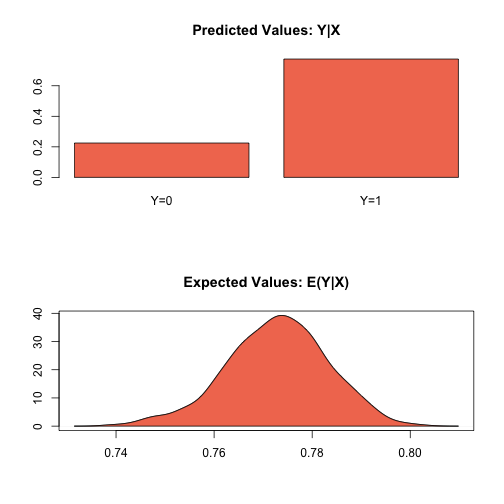
\includegraphics{unnamed-chunk-18-1.png}
\end{figure}

The cost of giving a range of values for \(\tau\) is that point
estimates are not available for quantities of interest. Instead,
quantities are presented as confidence intervals with significance less
than or equal to a specified level (e.g., at least 95\% of the
simulations are contained in the nominal 95\% confidence interval).


\paragraph{Model}
\label{zelig-relogit:model}\begin{itemize}
\item {} 
Like the standard logistic regression, the \emph{stochastic component} for
the rare events logistic regression is:
\begin{gather}
\begin{split}Y_i \; \sim \; \textrm{Bernoulli}(\pi_i),\end{split}\notag
\end{gather}
where \(Y_i\) is the binary dependent variable, and takes a value
of either 0 or 1.

\item {} 
The \emph{systematic component} is:
\begin{gather}
\begin{split}\pi_i \; = \; \frac{1}{1 + \exp(-x_i \beta)}.\end{split}\notag
\end{gather}
\item {} 
If the sample is generated via a case-control (or choice-based)
design, such as when drawing all events (or “cases”) and a sample
from the non-events (or “controls”) and going backwards to collect
the explanatory variables, you must correct for selecting on the
dependent variable. While the slope coefficients are approximately
unbiased, the constant term may be significantly biased. Zelig has
two methods for case control correction:
\begin{enumerate}
\item {} 
The “prior correction” method adjusts the intercept term. Let
\(\tau\) be the true population fraction of events,
\(\bar{y}\) the fraction of events in the sample, and
\(\hat{\beta_0}\) the uncorrected intercept term. The
corrected intercept \(\beta_0\) is:
\begin{gather}
\begin{split}\beta =  \hat{\beta_0} - \ln \left[ \bigg( \frac{1 - \tau}{\tau}
  \bigg) \bigg( \frac{\bar{y}}{1 - \bar{y}} \bigg) \right].\end{split}\notag
\end{gather}
\item {} 
The “weighting” method performs a weighted logistic regression to
correct for a case-control sampling design. Let the 1 subscript
denote observations for which the dependent variable is observed
as a 1, and the 0 subscript denote observations for which the
dependent variable is observed as a 0. Then the vector of weights
\(w_i\)
\begin{gather}
\begin{split}\begin{aligned}
w_1 &=& \frac{\tau}{\bar{y}} \\
w_0 &=& \frac{(1 - \tau)}{(1 - \bar{y})} \\
w_i &=& w_1 Y_i + w_0 (1 - Y_i)\end{aligned}\end{split}\notag
\end{gather}
\end{enumerate}

If \(\tau\) is unknown, you may alternatively specify an upper
and lower bound for the possible range of \(\tau\). In this case,
the relogit procedure uses “robust Bayesian” methods to generate a
confidence interval (rather than a point estimate) for each quantity
of interest. The nominal coverage of the confidence interval is at
least as great as the actual coverage.

\item {} 
By default, estimates of the the coefficients \(\beta\) are
bias-corrected to account for finite sample or rare events bias. In
addition, quantities of interest, such as predicted probabilities,
are also corrected of rare-events bias. If \(\widehat{\beta}\)
are the uncorrected logit coefficients and
bias(\(\widehat{\beta}\)) is the bias term, the corrected
coefficients \(\tilde{\beta}\) are
\begin{gather}
\begin{split}\widehat{\beta} - \textrm{bias}(\widehat{\beta}) = \tilde{\beta}\end{split}\notag
\end{gather}
The bias term is
\begin{gather}
\begin{split}\textrm{bias}(\widehat{\beta}) = (X'WX)^{-1} X'W \xi\end{split}\notag
\end{gather}
where
\begin{gather}
\begin{split}\begin{aligned}
\xi_i &=& 0.5 Q_{ii} \Big( (1 + w-1)\widehat{\pi}_i - w_1 \Big) \\
Q &=& X(X'WX)^{-1} X' \\
W = \textrm{diag}\{\widehat{\pi}_i (1 - \widehat{\pi}_i) w_i\}\end{aligned}\end{split}\notag
\end{gather}
where \(w_i\) and \(w_1\) are given in the “weighting”
section above.

\end{itemize}


\paragraph{Quantities of Interest}
\label{zelig-relogit:quantities-of-interest}\begin{itemize}
\item {} 
For either one or no \(\tau\):
\begin{itemize}
\item {} 
The expected values (qi\$ev) for the rare events logit are
simulations of the predicted probability
\begin{gather}
\begin{split}E(Y) = \pi_i =
    \frac{1}{1 + \exp(-x_i \beta)},\end{split}\notag
\end{gather}
given draws of \(\beta\) from its posterior.

\item {} 
The predicted value (qi\$pr) is a draw from a binomial distribution
with mean equal to the simulated \(\pi_i\).

\item {} 
The first difference (qi\$fd) is defined as
\begin{gather}
\begin{split}\textrm{FD} = \Pr(Y = 1 \mid x_1, \tau) - \Pr(Y = 1 \mid x, \tau).\end{split}\notag
\end{gather}
\item {} 
The risk ratio (qi\$rr) is defined as
\begin{gather}
\begin{split}\textrm{RR} = \Pr(Y = 1 \mid x_1, \tau) \ / \ \Pr(Y = 1 \mid x, \tau).\end{split}\notag
\end{gather}
\end{itemize}

\item {} 
For a range of \(\tau\) defined by \([\tau_1, \tau_2]\), each
of the quantities of interest are \(n \times 2\) matrices, which
report the lower and upper bounds, respectively, for a confidence
interval with nominal coverage at least as great as the actual
coverage. At worst, these bounds are conservative estimates for the
likely range for each quantity of interest. Please refer to for the
specific method of calculating bounded quantities of interest.

\item {} 
In conditional prediction models, the average expected treatment
effect (att.ev) for the treatment group is
\begin{gather}
\begin{split}\frac{1}{\sum_{i=1}^n t_i}\sum_{i:t_i=1}^n \left\{ Y_i(t_i=1) -
      E[Y_i(t_i=0)] \right\},\end{split}\notag
\end{gather}
where \(t_i\) is a binary explanatory variable defining the
treatment (\(t_i=1\)) and control (\(t_i=0\)) groups.
Variation in the simulations are due to uncertainty in simulating
\(E[Y_i(t_i=0)]\), the counterfactual expected value of
\(Y_i\) for observations in the treatment group, under the
assumption that everything stays the same except that the treatment
indicator is switched to \(t_i=0\).

\item {} 
In conditional prediction models, the average predicted treatment
effect (att.pr) for the treatment group is
\begin{gather}
\begin{split}\frac{1}{\sum_{i=1}^n t_i}\sum_{i:t_i=1}^n \left\{ Y_i(t_i=1) -
      \widehat{Y_i(t_i=0)} \right\},\end{split}\notag
\end{gather}
where \(t_i\) is a binary explanatory variable defining the
treatment (\(t_i=1\)) and control (\(t_i=0\)) groups.
Variation in the simulations are due to uncertainty in simulating
\(\widehat{Y_i(t_i=0)}\), the counterfactual predicted value of
\(Y_i\) for observations in the treatment group, under the
assumption that everything stays the same except that the treatment
indicator is switched to \(t_i=0\).

\end{itemize}


\paragraph{Output Values}
\label{zelig-relogit:output-values}
The output of each Zelig command contains useful information which you
may view. For example, if you run
\code{z.out \textless{}- zelig(y \textasciitilde{} x, model = relogit, data)}, then you may examine
the available information in \code{z.out} by using \code{names(z.out)}, see
the coefficients by using z.out\$coefficients, and a default summary of
information through \code{summary(z.out)}.


\paragraph{Differences with Stata Version}
\label{zelig-relogit:differences-with-stata-version}
The Stata version of ReLogit and the R implementation differ slightly in
their coefficient estimates due to differences in the matrix inversion
routines implemented in R and Stata. Zelig uses orthogonal-triangular
decomposition (through lm.influence()) to compute the bias term, which
is more numerically stable than standard matrix calculations.


\paragraph{See also}
\label{zelig-relogit:see-also}

\subsubsection{zelig-tobit}
\label{zelig-tobit:ztobit}\label{zelig-tobit::doc}\label{zelig-tobit:zelig-tobit}
Linear Regression for a Left-Censored Dependent Variable

Tobit regression estimates a linear regression model for a left-censored
dependent variable, where the dependent variable is censored from below.
While the classical tobit model has values censored at 0, you may select
another censoring point. For other linear regression models with fully
observed dependent variables, see Bayesian regression (), maximum
likelihood normal regression (), or least squares ().


\paragraph{Syntax}
\label{zelig-tobit:syntax}
\begin{Verbatim}[commandchars=\\\{\}]
z5 \PYG{o}{\PYGZlt{}\PYGZhy{}} ztobit\PYG{o}{\PYGZdl{}}new\PYG{p}{(}\PYG{p}{)}
z5\PYG{o}{\PYGZdl{}}zelig\PYG{p}{(}Y \PYG{o}{\PYGZti{}} X1 \PYG{o}{+} X2\PYG{p}{,} below \PYG{o}{=} \PYG{l+m}{0}\PYG{p}{,} above \PYG{o}{=} \PYG{k+kc}{Inf}\PYG{p}{,} data \PYG{o}{=} mydata\PYG{p}{)}
z5\PYG{o}{\PYGZdl{}}setx\PYG{p}{(}\PYG{p}{)}
z5\PYG{o}{\PYGZdl{}}sim\PYG{p}{(}\PYG{p}{)}
\end{Verbatim}

With the Zelig 4 compatibility wrappers:

\begin{Verbatim}[commandchars=\\\{\}]
z.out \PYG{o}{\PYGZlt{}\PYGZhy{}} zelig\PYG{p}{(}Y \PYG{o}{\PYGZti{}} X1 \PYG{o}{+} X2\PYG{p}{,} below \PYG{o}{=} \PYG{l+m}{0}\PYG{p}{,} above \PYG{o}{=} \PYG{k+kc}{Inf}\PYG{p}{,} model \PYG{o}{=} \PYG{l+s}{\PYGZdq{}}\PYG{l+s}{tobit\PYGZdq{}}\PYG{p}{,} data \PYG{o}{=} mydata\PYG{p}{)}
x.out \PYG{o}{\PYGZlt{}\PYGZhy{}} setx\PYG{p}{(}z.out\PYG{p}{)}
s.out \PYG{o}{\PYGZlt{}\PYGZhy{}} sim\PYG{p}{(}z.out\PYG{p}{,} x \PYG{o}{=} x.out\PYG{p}{)}
\end{Verbatim}


\paragraph{Inputs}
\label{zelig-tobit:inputs}
zelig() accepts the following arguments to specify how the dependent
variable is censored.
\begin{itemize}
\item {} 
\code{below}: (defaults to 0) The point at which the dependent variable
is censored from below. If any values in the dependent variable are
observed to be less than the censoring point, it is assumed that that
particular observation is censored from below at the observed value.
(See for a Bayesian implementation that supports both left and right
censoring.)

\item {} 
robust: defaults to FALSE. If TRUE, zelig() computes robust standard
errors based on sandwich estimators (see and ) and the options
selected in cluster.

\item {} 
cluster: if robust = TRUE, you may select a variable to define groups
of correlated observations. Let x3 be a variable that consists of
either discrete numeric values, character strings, or factors that
define strata. Then

\begin{Verbatim}[commandchars=\\\{\}]
\PYGZgt{} z.out \PYGZlt{}\PYGZhy{} zelig(y \PYGZti{} x1 + x2, robust = TRUE, cluster = \PYGZdq{}x3\PYGZdq{},
                 model = \PYGZdq{}tobit\PYGZdq{}, data = mydata)
\end{Verbatim}

means that the observations can be correlated within the strata
defined by the variable x3, and that robust standard errors should be
calculated according to those clusters. If robust = TRUE but cluster
is not specified, zelig() assumes that each observation falls into
its own cluster.

\end{itemize}

Zelig users may wish to refer to \code{help(survreg)} for more information.


\paragraph{Examples}
\label{zelig-tobit:examples}

\subparagraph{Basic Example}
\label{zelig-tobit:basic-example}
Attaching the sample dataset:

\begin{Verbatim}[commandchars=\\\{\}]
data\PYG{p}{(}tobin\PYG{p}{)}
\end{Verbatim}

Estimating linear regression using \code{tobit}:

\begin{Verbatim}[commandchars=\\\{\}]
z.out \PYG{o}{\PYGZlt{}\PYGZhy{}} zelig\PYG{p}{(}durable \PYG{o}{\PYGZti{}} age \PYG{o}{+} quant\PYG{p}{,} model \PYG{o}{=} \PYG{l+s}{\PYGZdq{}}\PYG{l+s}{tobit\PYGZdq{}}\PYG{p}{,} data \PYG{o}{=} tobin\PYG{p}{)}
\end{Verbatim}

\begin{Verbatim}[commandchars=\\\{\}]
\PYG{c}{\PYGZsh{}\PYGZsh{} How to cite this model in Zelig:}
\PYG{c}{\PYGZsh{}\PYGZsh{}   Kosuke Imai, Gary King, Olivia Lau. 2011.}
\PYG{c}{\PYGZsh{}\PYGZsh{}   tobit: Linear regression for Left\PYGZhy{}Censored Dependent Variable}
\PYG{c}{\PYGZsh{}\PYGZsh{}   in Kosuke Imai, Gary King, and Olivia Lau, \PYGZdq{}Zelig: Everyone\PYGZsq{}s Statistical Software,\PYGZdq{}}
\PYG{c}{\PYGZsh{}\PYGZsh{}   http://zeligproject.org/}
\end{Verbatim}

Setting values for the explanatory variables to their sample averages:

\begin{Verbatim}[commandchars=\\\{\}]
x.out \PYG{o}{\PYGZlt{}\PYGZhy{}} setx\PYG{p}{(}z.out\PYG{p}{)}
\end{Verbatim}

Simulating quantities of interest from the posterior distribution given \code{x.out}.

\begin{Verbatim}[commandchars=\\\{\}]
s.out1 \PYG{o}{\PYGZlt{}\PYGZhy{}} sim\PYG{p}{(}z.out\PYG{p}{,} x \PYG{o}{=} x.out\PYG{p}{)}
\end{Verbatim}

\begin{Verbatim}[commandchars=\\\{\}]
summary\PYG{p}{(}s.out1\PYG{p}{)}
\end{Verbatim}

\begin{Verbatim}[commandchars=\\\{\}]
\PYG{c}{\PYGZsh{}\PYGZsh{}}
\PYG{c}{\PYGZsh{}\PYGZsh{}  sim x :}
\PYG{c}{\PYGZsh{}\PYGZsh{}  \PYGZhy{}\PYGZhy{}\PYGZhy{}\PYGZhy{}\PYGZhy{}}
\PYG{c}{\PYGZsh{}\PYGZsh{} ev}
\PYG{c}{\PYGZsh{}\PYGZsh{}       mean        sd      50\PYGZpc{}      2.5\PYGZpc{}    97.5\PYGZpc{}}
\PYG{c}{\PYGZsh{}\PYGZsh{} 1 1.522538 0.6238672 1.476463 0.4294109 2.971289}
\PYG{c}{\PYGZsh{}\PYGZsh{} pv}
\PYG{c}{\PYGZsh{}\PYGZsh{}         mean       sd      50\PYGZpc{} 2.5\PYGZpc{}    97.5\PYGZpc{}}
\PYG{c}{\PYGZsh{}\PYGZsh{} [1,] 3.09644 3.898018 1.431842    0 12.69079}
\end{Verbatim}


\subparagraph{Simulating First Differences}
\label{zelig-tobit:simulating-first-differences}
Set explanatory variables to their default(mean/mode) values, with
high (80th percentile) and low (20th percentile) liquidity ratio
(\code{quant}):

\begin{Verbatim}[commandchars=\\\{\}]
x.high \PYG{o}{\PYGZlt{}\PYGZhy{}} setx\PYG{p}{(}z.out\PYG{p}{,} quant \PYG{o}{=} quantile\PYG{p}{(}tobin\PYG{o}{\PYGZdl{}}quant\PYG{p}{,} prob \PYG{o}{=} \PYG{l+m}{0.8}\PYG{p}{)}\PYG{p}{)}
x.low \PYG{o}{\PYGZlt{}\PYGZhy{}} setx\PYG{p}{(}z.out\PYG{p}{,} quant \PYG{o}{=} quantile\PYG{p}{(}tobin\PYG{o}{\PYGZdl{}}quant\PYG{p}{,} prob \PYG{o}{=} \PYG{l+m}{0.2}\PYG{p}{)}\PYG{p}{)}
\end{Verbatim}

Estimating the first difference for the effect of high versus low
liquidity ratio on duration(\code{durable}):

\begin{Verbatim}[commandchars=\\\{\}]
s.out2 \PYG{o}{\PYGZlt{}\PYGZhy{}} sim\PYG{p}{(}z.out\PYG{p}{,} x \PYG{o}{=} x.high\PYG{p}{,} x1 \PYG{o}{=} x.low\PYG{p}{)}
\end{Verbatim}

\begin{Verbatim}[commandchars=\\\{\}]
summary\PYG{p}{(}s.out2\PYG{p}{)}
\end{Verbatim}

\begin{Verbatim}[commandchars=\\\{\}]
\PYG{c}{\PYGZsh{}\PYGZsh{}}
\PYG{c}{\PYGZsh{}\PYGZsh{}  sim x :}
\PYG{c}{\PYGZsh{}\PYGZsh{}  \PYGZhy{}\PYGZhy{}\PYGZhy{}\PYGZhy{}\PYGZhy{}}
\PYG{c}{\PYGZsh{}\PYGZsh{} ev}
\PYG{c}{\PYGZsh{}\PYGZsh{}       mean        sd      50\PYGZpc{}     2.5\PYGZpc{}   97.5\PYGZpc{}}
\PYG{c}{\PYGZsh{}\PYGZsh{} 1 1.192813 0.7800701 1.070859 0.123258 3.16135}
\PYG{c}{\PYGZsh{}\PYGZsh{} pv}
\PYG{c}{\PYGZsh{}\PYGZsh{}          mean       sd      50\PYGZpc{} 2.5\PYGZpc{}    97.5\PYGZpc{}}
\PYG{c}{\PYGZsh{}\PYGZsh{} [1,] 3.132773 4.150502 1.323289    0 14.14609}
\PYG{c}{\PYGZsh{}\PYGZsh{}}
\PYG{c}{\PYGZsh{}\PYGZsh{}  sim x1 :}
\PYG{c}{\PYGZsh{}\PYGZsh{}  \PYGZhy{}\PYGZhy{}\PYGZhy{}\PYGZhy{}\PYGZhy{}}
\PYG{c}{\PYGZsh{}\PYGZsh{} ev}
\PYG{c}{\PYGZsh{}\PYGZsh{}       mean        sd      50\PYGZpc{}      2.5\PYGZpc{}    97.5\PYGZpc{}}
\PYG{c}{\PYGZsh{}\PYGZsh{} 1 2.023184 0.9289575 1.907224 0.5365063 4.132607}
\PYG{c}{\PYGZsh{}\PYGZsh{} pv}
\PYG{c}{\PYGZsh{}\PYGZsh{}          mean       sd     50\PYGZpc{} 2.5\PYGZpc{}    97.5\PYGZpc{}}
\PYG{c}{\PYGZsh{}\PYGZsh{} [1,] 3.724101 4.401357 2.11134    0 15.06014}
\PYG{c}{\PYGZsh{}\PYGZsh{} fd}
\PYG{c}{\PYGZsh{}\PYGZsh{}        mean       sd       50\PYGZpc{}      2.5\PYGZpc{}    97.5\PYGZpc{}}
\PYG{c}{\PYGZsh{}\PYGZsh{} 1 0.8303709 1.143904 0.7664756 \PYGZhy{}1.441829 3.200998}
\end{Verbatim}

\begin{Verbatim}[commandchars=\\\{\}]
plot\PYG{p}{(}s.out1\PYG{p}{)}
\end{Verbatim}
\begin{figure}[htbp]
\centering
\capstart

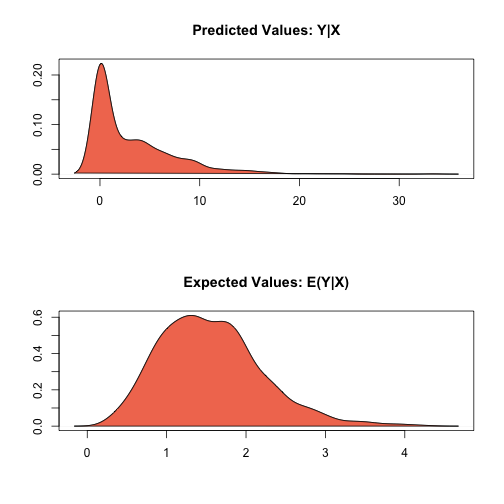
\includegraphics{Zelig-tobit-1.png}
\caption{Zelig-tobit}\end{figure}


\paragraph{Model}
\label{zelig-tobit:model}\begin{itemize}
\item {} 
Let \(Y_i^*\) be a latent dependent variable which is distributed
with \emph{stochastic} component
\begin{gather}
\begin{split}\begin{aligned}
Y_i^* & \sim & \textrm{Normal}(\mu_i, \sigma^2) \\\end{aligned}\end{split}\notag
\end{gather}
where \(\mu_i\) is a vector means and \(\sigma^2\) is a
scalar variance parameter. \(Y_i^*\) is not directly observed,
however. Rather we observed \(Y_i\) which is defined as:
\begin{gather}
\begin{split}Y_i = \left\{
\begin{array}{lcl}
Y_i^*  &\textrm{if} & c <Y_i^* \\
c    &\textrm{if} & c \ge Y_i^*
\end{array}\right.\end{split}\notag
\end{gather}
where \(c\) is the lower bound below which \(Y_i^*\) is
censored.

\item {} 
The \emph{systematic component} is given by
\begin{gather}
\begin{split}\begin{aligned}
\mu_{i} &=& x_{i} \beta,\end{aligned}\end{split}\notag
\end{gather}
where \(x_{i}\) is the vector of \(k\) explanatory variables
for observation \(i\) and \(\beta\) is the vector of
coefficients.

\end{itemize}


\paragraph{Quantities of Interest}
\label{zelig-tobit:quantities-of-interest}\begin{itemize}
\item {} 
The expected values (\code{qi\$ev}) for the tobit regression model are
the same as the expected value of \(Y*\):
\begin{gather}
\begin{split}E(Y^* | X) = \mu_{i} = x_{i} \beta\end{split}\notag
\end{gather}
\item {} 
The first difference (\code{qi\$fd}) for the tobit regression model is
defined as
\begin{gather}
\begin{split}\begin{aligned}
\text{FD}=E(Y^* \mid x_{1}) - E(Y^* \mid x).\end{aligned}\end{split}\notag
\end{gather}
\item {} 
In conditional prediction models, the average expected treatment
effect (\code{qi\$att.ev}) for the treatment group is
\begin{gather}
\begin{split}\begin{aligned}
\frac{1}{\sum t_{i}}\sum_{i:t_{i}=1}[E[Y^*_{i}(t_{i}=1)]-E[Y^*_{i}(t_{i}=0)]],\end{aligned}\end{split}\notag
\end{gather}
where \(t_{i}\) is a binary explanatory variable defining the
treatment (\(t_{i}=1\)) and control (\(t_{i}=0\)) groups.

\end{itemize}


\paragraph{Output Values}
\label{zelig-tobit:output-values}
The output of each Zelig command contains useful information which you
may view. For example, if you run:

\begin{Verbatim}[commandchars=\\\{\}]
z.out \PYG{o}{\PYGZlt{}\PYGZhy{}} zelig\PYG{p}{(}y \PYG{o}{\PYGZti{}} x\PYG{p}{,} model \PYG{o}{=} \PYG{l+s}{\PYGZdq{}}\PYG{l+s}{tobit\PYGZdq{}}\PYG{p}{,} data\PYG{p}{)}
\end{Verbatim}

then you may examine the available information in {\color{red}\bfseries{}{}`{}`}z.out{}`.


\paragraph{See also}
\label{zelig-tobit:see-also}
The tobit function is part of the survival library by Terry Therneau,
ported to R by Thomas Lumley. Advanced users may wish to refer to
\code{help(survfit)} in the survival library.


\subsubsection{zelig-factorbayes}
\label{zelig-factorbayes:zelig-factorbayes}\label{zelig-factorbayes::doc}\label{zelig-factorbayes:zfactorbayes}
Given some unobserved explanatory variables and observed dependent
variables, the Normal theory factor analysis model estimates the latent
factors. The model is implemented using a Markov Chain Monte Carlo
algorithm (Gibbs sampling with data augmentation). For factor analysis
with ordinal dependent variables, see ordered factor analysis (), and
for a mix of types of dependent variables, see the mixed factor analysis
model ().


\paragraph{Syntax}
\label{zelig-factorbayes:syntax}
With reference classes:

\begin{Verbatim}[commandchars=\\\{\}]
z5 \PYG{o}{\PYGZlt{}\PYGZhy{}} zfactorbayes\PYG{o}{\PYGZdl{}}new\PYG{p}{(}\PYG{p}{)}
z5\PYG{o}{\PYGZdl{}}zelig\PYG{p}{(}cbind\PYG{p}{(}Y1 \PYG{p}{,}Y2\PYG{p}{,} Y3\PYG{p}{)} \PYG{o}{\PYGZti{}} \PYG{k+kc}{NULL}\PYG{p}{,} factors \PYG{o}{=} \PYG{l+m}{2}\PYG{p}{,}
         model \PYG{o}{=} \PYG{l+s}{\PYGZdq{}}\PYG{l+s}{factor.bayes\PYGZdq{}}\PYG{p}{,} data \PYG{o}{=} mydata\PYG{p}{)}
\end{Verbatim}

With the Zelig 4 compatibility wrappers:

\begin{Verbatim}[commandchars=\\\{\}]
z.out \PYG{o}{\PYGZlt{}\PYGZhy{}} zelig\PYG{p}{(}cbind\PYG{p}{(}Y1 \PYG{p}{,}Y2\PYG{p}{,} Y3\PYG{p}{)} \PYG{o}{\PYGZti{}} \PYG{k+kc}{NULL}\PYG{p}{,} factors \PYG{o}{=} \PYG{l+m}{2}\PYG{p}{,}
               model \PYG{o}{=} \PYG{l+s}{\PYGZdq{}}\PYG{l+s}{factor.bayes\PYGZdq{}}\PYG{p}{,} data \PYG{o}{=} mydata\PYG{p}{)}
\end{Verbatim}


\paragraph{Inputs}
\label{zelig-factorbayes:inputs}
zelig() takes the following functions for factor.bayes:
\begin{itemize}
\item {} 
\code{Y1}, \code{Y2}, and \code{Y3}: variables of interest in factor analysis
(manifest variables), assumed to be normally distributed. The model
requires a minimum of three manifest variables.

\item {} 
\code{factors}: number of the factors to be fitted (defaults to 2).

\end{itemize}


\paragraph{Additional Inputs}
\label{zelig-factorbayes:additional-inputs}
In addition, zelig() accepts the following additional arguments for
model specification:
\begin{itemize}
\item {} 
\code{lambda.constraints}: list containing the equality or inequality
constraints on the factor loadings. Choose from one of the following
forms:
\begin{itemize}
\item {} 
varname = list(): by default, no constraints are imposed.

\item {} 
\code{varname = list(d, c)}: constrains the \(d\)th loading for
the variable named \code{varname} to be equal to \code{c}.

\item {} 
\code{varname = list(d, +)}: constrains the \(d\)th loading for
the variable named \code{varname} to be positive;

\item {} 
\code{varname = list(d, -)}: constrains the \(d\)th loading for
the variable named \code{varname} to be negative.

\end{itemize}

\item {} 
\code{std.var}: defaults to FALSE (manifest variables are rescaled to
zero mean, but retain observed variance). If \code{TRUE}, the manifest
variables are rescaled to be mean zero and unit variance.

\end{itemize}

In addition, zelig() accepts the following additional inputs for
bayes.factor:
\begin{itemize}
\item {} 
\code{burnin}: number of the initial MCMC iterations to be discarded
(defaults to 1,000).

\item {} 
\code{mcmc}: number of the MCMC iterations after burnin (defaults to
20,000).

\item {} 
\code{thin}: thinning interval for the Markov chain. Only every
\code{thin}-th draw from the Markov chain is kept. The value of \code{mcmc}
must be divisible by this value. The default value is 1.

\item {} 
\code{verbose}: defaults to FALSE. If \code{TRUE}, the progress of the
sampler (every \(10\%\)) is printed to the screen.

\item {} 
\code{seed}: seed for the random number generator. The default is \code{NA}
which corresponds to a random seed 12345.

\item {} 
\code{Lambda.start}: starting values of the factor loading matrix
\(\Lambda\), either a scalar (all unconstrained loadings are set
to that value), or a matrix with compatible dimensions. The default
is \code{NA}, where the start value are set to be 0 for unconstrained
factor loadings, and 0.5 or \(-\)0.5 for constrained factor
loadings (depending on the nature of the constraints).

\item {} 
\code{Psi.start}: starting values for the uniquenesses, either a scalar
(the starting values for all diagonal elements of \(\Psi\) are
set to be this value), or a vector with length equal to the number of
manifest variables. In the latter case, the starting values of the
diagonal elements of \(\Psi\) take the values of \code{Psi.start}.
The default value is \code{NA} where the starting values of the all the
uniquenesses are set to be 0.5.

\item {} 
\code{store.lambda}: defaults to TRUE, which stores the posterior draws
of the factor loadings.

\item {} 
\code{store.scores}: defaults to FALSE. If TRUE, stores the posterior
draws of the factor scores. (Storing factor scores may take large
amount of memory for a large number of draws or observations.)

\end{itemize}

The model also accepts the following additional arguments to specify
prior parameters:
\begin{itemize}
\item {} 
\code{l0}: mean of the Normal prior for the factor loadings, either a
scalar or a matrix with the same dimensions as \(\Lambda\). If a
scalar value, that value will be the prior mean for all the factor
loadings. Defaults to 0.

\item {} 
\code{L0}: precision parameter of the Normal prior for the factor
loadings, either a scalar or a matrix with the same dimensions as
\(\Lambda\). If \code{L0} takes a scalar value, then the precision
matrix will be a diagonal matrix with the diagonal elements set to
that value. The default value is 0, which leads to an improper prior.

\item {} 
\code{a0}: the shape parameter of the Inverse Gamma prior for the
uniquenesses is \code{a0/2}. It can take a scalar value or a vector. The
default value is 0.001.

\item {} 
\code{b0}: the shape parameter of the Inverse Gamma prior for the
uniquenesses is \code{b0/2}. It can take a scalar value or a vector. The
default value is 0.001.

\end{itemize}

Zelig users may wish to refer to \code{help(MCMCfactanal)} for more
information.


\paragraph{Example}
\label{zelig-factorbayes:example}
Attaching the sample dataset:

\begin{Verbatim}[commandchars=\\\{\}]
data\PYG{p}{(}swiss\PYG{p}{)}
names\PYG{p}{(}swiss\PYG{p}{)} \PYG{o}{\PYGZlt{}\PYGZhy{}} c\PYG{p}{(}\PYG{l+s}{\PYGZdq{}}\PYG{l+s}{Fert\PYGZdq{}}\PYG{p}{,} \PYG{l+s}{\PYGZdq{}}\PYG{l+s}{Agr\PYGZdq{}}\PYG{p}{,} \PYG{l+s}{\PYGZdq{}}\PYG{l+s}{Exam\PYGZdq{}}\PYG{p}{,} \PYG{l+s}{\PYGZdq{}}\PYG{l+s}{Educ\PYGZdq{}}\PYG{p}{,} \PYG{l+s}{\PYGZdq{}}\PYG{l+s}{Cath\PYGZdq{}}\PYG{p}{,} \PYG{l+s}{\PYGZdq{}}\PYG{l+s}{InfMort\PYGZdq{}}\PYG{p}{)}
\end{Verbatim}

Factor analysis:

\begin{Verbatim}[commandchars=\\\{\}]
z.out \PYG{o}{\PYGZlt{}\PYGZhy{}} zelig\PYG{p}{(}cbind\PYG{p}{(}Agr\PYG{p}{,} Exam\PYG{p}{,} Educ\PYG{p}{,} Cath\PYG{p}{,} InfMort\PYG{p}{)} \PYG{o}{\PYGZti{}} \PYG{k+kc}{NULL}\PYG{p}{,}
               model \PYG{o}{=} \PYG{l+s}{\PYGZdq{}}\PYG{l+s}{factor.bayes\PYGZdq{}}\PYG{p}{,} data \PYG{o}{=} swiss\PYG{p}{,} factors \PYG{o}{=} \PYG{l+m}{2}\PYG{p}{,} verbose \PYG{o}{=} \PYG{k+kc}{TRUE}\PYG{p}{,}
               a0 \PYG{o}{=} \PYG{l+m}{1}\PYG{p}{,} b0 \PYG{o}{=} \PYG{l+m}{0.15}\PYG{p}{,} burnin \PYG{o}{=} \PYG{l+m}{5000}\PYG{p}{,} mcmc \PYG{o}{=} \PYG{l+m}{50000}\PYG{p}{)}
\end{Verbatim}

Checking for convergence before summarizing the estimates:

\begin{Verbatim}[commandchars=\\\{\}]
algor \PYG{o}{\PYGZlt{}\PYGZhy{}} try\PYG{p}{(}geweke.diag\PYG{p}{(}z.out\PYG{o}{\PYGZdl{}}coefficients\PYG{p}{)}\PYG{p}{,} silent\PYG{o}{=}\PYG{k+kVariable}{T}\PYG{p}{)}
\PYG{k+kr}{if} \PYG{p}{(}class\PYG{p}{(}algor\PYG{p}{)} \PYG{o}{==} \PYG{l+s}{\PYGZdq{}}\PYG{l+s}{try\PYGZhy{}error\PYGZdq{}}\PYG{p}{)}
    print\PYG{p}{(}algor\PYG{p}{)}
\end{Verbatim}

Since the algorithm did not converge, we now add some constraints on
\(\Lambda\) to optimize the algorithm:

\begin{Verbatim}[commandchars=\\\{\}]
z.out \PYG{o}{\PYGZlt{}\PYGZhy{}} zelig\PYG{p}{(}cbind\PYG{p}{(}Agr\PYG{p}{,} Exam\PYG{p}{,} Educ\PYG{p}{,} Cath\PYG{p}{,} InfMort\PYG{p}{)} \PYG{o}{\PYGZti{}} \PYG{k+kc}{NULL}\PYG{p}{,}
               model \PYG{o}{=} \PYG{l+s}{\PYGZdq{}}\PYG{l+s}{factor.bayes\PYGZdq{}}\PYG{p}{,} data \PYG{o}{=} swiss\PYG{p}{,} factors \PYG{o}{=} \PYG{l+m}{2}\PYG{p}{,}
               lambda.constraints \PYG{o}{=} list\PYG{p}{(}Exam \PYG{o}{=} list\PYG{p}{(}\PYG{l+m}{1}\PYG{p}{,}\PYG{l+s}{\PYGZdq{}}\PYG{l+s}{+\PYGZdq{}}\PYG{p}{)}\PYG{p}{,}
                   Exam \PYG{o}{=} list\PYG{p}{(}\PYG{l+m}{2}\PYG{p}{,}\PYG{l+s}{\PYGZdq{}}\PYG{l+s}{\PYGZhy{}\PYGZdq{}}\PYG{p}{)}\PYG{p}{,} Educ \PYG{o}{=} c\PYG{p}{(}\PYG{l+m}{2}\PYG{p}{,} \PYG{l+m}{0}\PYG{p}{)}\PYG{p}{,}
                   InfMort \PYG{o}{=} c\PYG{p}{(}\PYG{l+m}{1}\PYG{p}{,} \PYG{l+m}{0}\PYG{p}{)}\PYG{p}{)}\PYG{p}{,}
               verbose \PYG{o}{=} \PYG{k+kc}{TRUE}\PYG{p}{,} a0 \PYG{o}{=} \PYG{l+m}{1}\PYG{p}{,} b0 \PYG{o}{=} \PYG{l+m}{0.15}\PYG{p}{,}
               burnin \PYG{o}{=} \PYG{l+m}{5000}\PYG{p}{,} mcmc \PYG{o}{=} \PYG{l+m}{50000}\PYG{p}{)}
geweke.diag\PYG{p}{(}z.out\PYG{o}{\PYGZdl{}}coefficients\PYG{p}{)}
heidel.diag\PYG{p}{(}z.out\PYG{o}{\PYGZdl{}}coefficients\PYG{p}{)}
raftery.diag\PYG{p}{(}z.out\PYG{o}{\PYGZdl{}}coefficients\PYG{p}{)}
summary\PYG{p}{(}z.out\PYG{p}{)}
\end{Verbatim}


\paragraph{Model}
\label{zelig-factorbayes:model}
Suppose for observation \(i\) we observe \(K\) variables and
hypothesize that there are \(d\) underlying factors such that:
\begin{gather}
\begin{split}\begin{aligned}
Y_i = \Lambda \phi_i+\epsilon_i\end{aligned}\end{split}\notag
\end{gather}
where \(Y_{i}\) is the vector of \(K\) manifest variables for
observation \(i\). \(\Lambda\) is the \(K \times d\) factor
loading matrix and \(\phi_i\) is the \(d\)-vector of latent
factor scores. Both \(\Lambda\) and \(\phi\) need to be
estimated.
\begin{itemize}
\item {} 
The \emph{stochastic component} is given by:
\begin{gather}
\begin{split}\begin{aligned}
\epsilon_{i}  \sim \textrm{Normal}(0, \Psi).\end{aligned}\end{split}\notag
\end{gather}
where \(\Psi\) is a diagonal, positive definite matrix. The
diagonal elements of \(\Psi\) are referred to as uniquenesses.

\item {} 
The \emph{systematic component} is given by
\begin{gather}
\begin{split}\begin{aligned}
\mu_i = E(Y_i) = \Lambda\phi_i\end{aligned}\end{split}\notag
\end{gather}
\item {} 
The independent conjugate \emph{prior} for each \(\Lambda_{ij}\) is
given by
\begin{gather}
\begin{split}\begin{aligned}
\Lambda_{ij} \sim \textrm{Normal}(l_{0_{ij}}, L_{0_{ij}}^{-1})
\textrm{ for } i=1,\ldots, k; \quad j=1,\ldots, d. \end{aligned}\end{split}\notag
\end{gather}
\item {} 
The independent conjugate \emph{prior} for each \(\Psi_{ii}\) is given
by
\begin{gather}
\begin{split}\begin{aligned}
\Psi_{ii} \sim \textrm{InverseGamma}(\frac{a_0}{2}, \frac{b_0}{2}), \textrm{ for }
i = 1, \ldots, k.\end{aligned}\end{split}\notag
\end{gather}
\item {} 
The \emph{prior} for \(\phi_i\) is
\begin{gather}
\begin{split}\begin{aligned}
\phi_i &\sim& \textrm{Normal}(0, I_d), \textrm{ for } i = 1, \ldots, n.\end{aligned}\end{split}\notag
\end{gather}
where \(I_d\) is a :math:{}` dtimes d {}` identity matrix.

\end{itemize}


\paragraph{Output Values}
\label{zelig-factorbayes:output-values}
The output of each Zelig command contains useful information which you
may view. For example, if you run:

\begin{Verbatim}[commandchars=\\\{\}]
z.out \PYG{o}{\PYGZlt{}\PYGZhy{}} zelig\PYG{p}{(}cbind\PYG{p}{(}Y1\PYG{p}{,} Y2\PYG{p}{,} Y3\PYG{p}{)}\PYG{p}{,} model \PYG{o}{=} \PYG{l+s}{\PYGZdq{}}\PYG{l+s}{factor.bayes\PYGZdq{}}\PYG{p}{,} data\PYG{p}{)}
\end{Verbatim}

then you may examine the available information in \code{z.out} by using
\code{names(z.out)}, see the draws from the posterior distribution of the
\code{coefficients} by using \code{z.out\$coefficients}, and view a default
summary of information through \code{summary(z.out)}. Other elements
available through the \code{\$} operator are listed below.
\begin{itemize}
\item {} 
From the \code{zelig()} output object \code{z.out}, you may extract:
\begin{itemize}
\item {} 
\code{coefficients}: draws from the posterior distributions of the
estimated factor loadings and the uniquenesses. If
\code{store.scores = TRUE}, the estimated factors scores are also
contained in \code{coefficients}.

\item {} 
\code{data}: the name of the input data frame.

\item {} 
\code{seed}: the random seed used in the model.

\end{itemize}

\item {} 
Since there are no explanatory variables, the \code{sim()} procedure is
not applicable for factor analysis models.

\end{itemize}


\subsubsection{zelig-mlogitbayes}
\label{zelig-mlogitbayes:zmlogitbayes}\label{zelig-mlogitbayes::doc}\label{zelig-mlogitbayes:zelig-mlogitbayes}
Use Bayesian multinomial logistic regression to model unordered
categorical variables. The dependent variable may be in the format of
either character strings or integer values. The model is estimated via a
random walk Metropolis algorithm or a slice sampler. See for the
maximum-likelihood estimation of this model.


\paragraph{Syntax}
\label{zelig-mlogitbayes:syntax}
With reference classes:

\begin{Verbatim}[commandchars=\\\{\}]
z5 \PYG{o}{\PYGZlt{}\PYGZhy{}} zmlogitbayes\PYG{o}{\PYGZdl{}}new\PYG{p}{(}\PYG{p}{)}
z5\PYG{o}{\PYGZdl{}}zelig\PYG{p}{(}Y \PYG{o}{\PYGZti{}} X1 \PYG{o}{+} X2\PYG{p}{,} data \PYG{o}{=} mydata\PYG{p}{)}
z5\PYG{o}{\PYGZdl{}}setx\PYG{p}{(}\PYG{p}{)}
z5\PYG{o}{\PYGZdl{}}sim\PYG{p}{(}\PYG{p}{)}
\end{Verbatim}

With the Zelig 4 compatibility wrappers:

\begin{Verbatim}[commandchars=\\\{\}]
z.out \PYG{o}{\PYGZlt{}\PYGZhy{}} zelig\PYG{p}{(}Y \PYG{o}{\PYGZti{}} X1 \PYG{o}{+} X2\PYG{p}{,} model \PYG{o}{=} \PYG{l+s}{\PYGZdq{}}\PYG{l+s}{mlogit.bayes\PYGZdq{}}\PYG{p}{,} data \PYG{o}{=} mydata\PYG{p}{)}
x.out \PYG{o}{\PYGZlt{}\PYGZhy{}} setx\PYG{p}{(}z.out\PYG{p}{)}
s.out \PYG{o}{\PYGZlt{}\PYGZhy{}} sim\PYG{p}{(}z.out\PYG{p}{,} x \PYG{o}{=} x.out\PYG{p}{)}
\end{Verbatim}


\paragraph{Additional Inputs}
\label{zelig-mlogitbayes:additional-inputs}
zelig() accepts the following arguments for mlogit.bayes:
\begin{itemize}
\item {} 
\code{baseline}: either a character string or numeric value (equal to
one of the observed values in the dependent variable) specifying a
baseline category. The default value is \code{NA} which sets the
baseline to the first alphabetical or numerical unique value of the
dependent variable.

\end{itemize}

The model accepts the following additional arguments to monitor the
Markov chains:
\begin{itemize}
\item {} 
\code{burnin}: number of the initial MCMC iterations to be discarded
(defaults to 1,000).

\item {} 
\code{mcmc}: number of the MCMC iterations after burnin (defaults to
10,000).

\item {} 
\code{thin}: thinning interval for the Markov chain. Only every
\code{thin}-th draw from the Markov chain is kept. The value of \code{mcmc}
must be divisible by this value. The default value is 1.

\item {} 
\code{mcmc.method}: either “MH” or “slice”, specifying whether to use
Metropolis Algorithm or slice sampler. The default value is \code{MH}.

\item {} 
\code{tune}: tuning parameter for the Metropolis-Hasting step, either a
scalar or a numeric vector (for \(k\) coefficients, enter a
\(k\) vector). The tuning parameter should be set such that the
acceptance rate is satisfactory (between 0.2 and 0.5). The default
value is 1.1.

\item {} 
\code{verbose}: defaults to \code{FALSE}. If \code{TRUE}, the progress of the
sampler (every \(10\%\)) is printed to the screen.

\item {} 
\code{seed}: seed for the random number generator. The default is \code{NA}
which corresponds to a random seed of 12345.

\item {} 
\code{beta.start}: starting values for the Markov chain, either a scalar
or a vector (for \(k\) coefficients, enter a \(k\) vector).
The default is \code{NA} where the maximum likelihood estimates are used
as the starting values.

\end{itemize}

Use the following arguments to specify the priors for the model:
\begin{itemize}
\item {} 
\code{b0}: prior mean for the coefficients, either a scalar or vector.
If a scalar, that value will be the prior mean for all the
coefficients. The default is 0.

\item {} 
\code{B0}: prior precision parameter for the coefficients, either a
square matrix with the dimensions equal to the number of coefficients
or a scalar. If a scalar, that value times an identity matrix will be
the prior precision parameter. The default is 0 which leads to an
improper prior.

\end{itemize}

Zelig users may wish to refer to \code{help(MCMCmnl)} for more information.


\paragraph{Examples}
\label{zelig-mlogitbayes:examples}

\subparagraph{Basic Example}
\label{zelig-mlogitbayes:basic-example}
Attaching the sample dataset:

\begin{Verbatim}[commandchars=\\\{\}]
data\PYG{p}{(}mexico\PYG{p}{)}
\end{Verbatim}

Estimating multinomial logistics regression using \code{mlogit.bayes}:

\begin{Verbatim}[commandchars=\\\{\}]
z.out \PYG{o}{\PYGZlt{}\PYGZhy{}} zelig\PYG{p}{(}vote88 \PYG{o}{\PYGZti{}} pristr \PYG{o}{+} othcok \PYG{o}{+} othsocok\PYG{p}{,}
               model \PYG{o}{=} \PYG{l+s}{\PYGZdq{}}\PYG{l+s}{mlogit.bayes\PYGZdq{}}\PYG{p}{,} data \PYG{o}{=} mexico\PYG{p}{,}
               verbose \PYG{o}{=} \PYG{k+kc}{FALSE}\PYG{p}{)}
\end{Verbatim}

\begin{Verbatim}[commandchars=\\\{\}]
\PYG{c}{\PYGZsh{}\PYGZsh{} Calculating MLEs and large sample var\PYGZhy{}cov matrix.}
\PYG{c}{\PYGZsh{}\PYGZsh{} This may take a moment...}
\PYG{c}{\PYGZsh{}\PYGZsh{} Inverting Hessian to get large sample var\PYGZhy{}cov matrix.}
\end{Verbatim}

\begin{Verbatim}[commandchars=\\\{\}]
\PYG{c}{\PYGZsh{}\PYGZsh{} Warning in if (mcmc.method == \PYGZdq{}RWM\PYGZdq{}) \PYGZob{}: the condition has length \PYGZgt{} 1 and}
\PYG{c}{\PYGZsh{}\PYGZsh{} only the first element will be used}
\end{Verbatim}

\begin{Verbatim}[commandchars=\\\{\}]
\PYG{c}{\PYGZsh{}\PYGZsh{} Warning in if (mcmc.method == \PYGZdq{}IndMH\PYGZdq{}) \PYGZob{}: the condition has length \PYGZgt{} 1 and}
\PYG{c}{\PYGZsh{}\PYGZsh{} only the first element will be used}
\end{Verbatim}

\begin{Verbatim}[commandchars=\\\{\}]
\PYG{c}{\PYGZsh{}\PYGZsh{} How to cite this model in Zelig:}
\PYG{c}{\PYGZsh{}\PYGZsh{}   Ben Goodrich, Ying Lu. 2013.}
\PYG{c}{\PYGZsh{}\PYGZsh{}   mlogitbayes: Bayesian Multinomial Logistic Regression for Dependent Variables with Unordered Categorical Values}
\PYG{c}{\PYGZsh{}\PYGZsh{}   in Kosuke Imai, Gary King, and Olivia Lau, \PYGZdq{}Zelig: Everyone\PYGZsq{}s Statistical Software,\PYGZdq{}}
\PYG{c}{\PYGZsh{}\PYGZsh{}   http://zeligproject.org/}
\end{Verbatim}

Checking for convergence before summarizing the estimates:

\begin{Verbatim}[commandchars=\\\{\}]
raftery.diag\PYG{p}{(}z.out\PYG{o}{\PYGZdl{}}coefficients\PYG{p}{)}
\end{Verbatim}

\begin{Verbatim}[commandchars=\\\{\}]
summary\PYG{p}{(}z.out\PYG{p}{)}
\end{Verbatim}

Setting values for the explanatory variables to their sample
averages:

\begin{Verbatim}[commandchars=\\\{\}]
x.out \PYG{o}{\PYGZlt{}\PYGZhy{}} setx\PYG{p}{(}z.out\PYG{p}{)}
\end{Verbatim}

Simulating quantities of interest from the posterior distribution
given \code{x.out}.

\begin{Verbatim}[commandchars=\\\{\}]
s.out1 \PYG{o}{\PYGZlt{}\PYGZhy{}} sim\PYG{p}{(}z.out\PYG{p}{,} x \PYG{o}{=} x.out\PYG{p}{)}
summary\PYG{p}{(}s.out1\PYG{p}{)}
\end{Verbatim}

\begin{Verbatim}[commandchars=\\\{\}]
\PYG{c}{\PYGZsh{}\PYGZsh{}}
\PYG{c}{\PYGZsh{}\PYGZsh{}  sim x :}
\PYG{c}{\PYGZsh{}\PYGZsh{}  \PYGZhy{}\PYGZhy{}\PYGZhy{}\PYGZhy{}\PYGZhy{}}
\PYG{c}{\PYGZsh{}\PYGZsh{} ev}
\PYG{c}{\PYGZsh{}\PYGZsh{}             mean         sd       50\PYGZpc{}      2.5\PYGZpc{}     97.5\PYGZpc{}}
\PYG{c}{\PYGZsh{}\PYGZsh{} P(Y=1) 0.5613368 0.01592425 0.5615034 0.5306640 0.5914963}
\PYG{c}{\PYGZsh{}\PYGZsh{} P(Y=2) 0.2099124 0.01273148 0.2098424 0.1854312 0.2350891}
\PYG{c}{\PYGZsh{}\PYGZsh{} P(Y=3) 0.2287508 0.01360126 0.2285987 0.2033590 0.2558153}
\PYG{c}{\PYGZsh{}\PYGZsh{} pv}
\PYG{c}{\PYGZsh{}\PYGZsh{} qi}
\PYG{c}{\PYGZsh{}\PYGZsh{}      1      2      3}
\PYG{c}{\PYGZsh{}\PYGZsh{} 0.5544 0.2155 0.2301}
\end{Verbatim}


\subparagraph{Simulating First Differences}
\label{zelig-mlogitbayes:simulating-first-differences}
Estimating the first difference (and risk ratio) in the
probabilities of voting different candidates when \code{pristr} (the
strength of the PRI) is set to be weak (equal to 1) versus strong
(equal to 3) while all the other variables held at their default
values.

\begin{Verbatim}[commandchars=\\\{\}]
x.weak \PYG{o}{\PYGZlt{}\PYGZhy{}} setx\PYG{p}{(}z.out\PYG{p}{,} pristr \PYG{o}{=} \PYG{l+m}{1}\PYG{p}{)}
x.strong \PYG{o}{\PYGZlt{}\PYGZhy{}} setx\PYG{p}{(}z.out\PYG{p}{,} pristr \PYG{o}{=} \PYG{l+m}{3}\PYG{p}{)}
s.out2 \PYG{o}{\PYGZlt{}\PYGZhy{}} sim\PYG{p}{(}z.out\PYG{p}{,} x \PYG{o}{=} x.strong\PYG{p}{,} x1 \PYG{o}{=} x.weak\PYG{p}{)}
summary\PYG{p}{(}s.out2\PYG{p}{)}
\end{Verbatim}

\begin{Verbatim}[commandchars=\\\{\}]
\PYG{c}{\PYGZsh{}\PYGZsh{}}
\PYG{c}{\PYGZsh{}\PYGZsh{}  sim x :}
\PYG{c}{\PYGZsh{}\PYGZsh{}  \PYGZhy{}\PYGZhy{}\PYGZhy{}\PYGZhy{}\PYGZhy{}}
\PYG{c}{\PYGZsh{}\PYGZsh{} ev}
\PYG{c}{\PYGZsh{}\PYGZsh{}             mean         sd       50\PYGZpc{}      2.5\PYGZpc{}     97.5\PYGZpc{}}
\PYG{c}{\PYGZsh{}\PYGZsh{} P(Y=1) 0.7156880 0.02127842 0.7158103 0.6725681 0.7561260}
\PYG{c}{\PYGZsh{}\PYGZsh{} P(Y=2) 0.1270237 0.01458077 0.1265905 0.1000858 0.1562571}
\PYG{c}{\PYGZsh{}\PYGZsh{} P(Y=3) 0.1572883 0.01646202 0.1568142 0.1260809 0.1909916}
\PYG{c}{\PYGZsh{}\PYGZsh{} pv}
\PYG{c}{\PYGZsh{}\PYGZsh{} qi}
\PYG{c}{\PYGZsh{}\PYGZsh{}      1      2      3}
\PYG{c}{\PYGZsh{}\PYGZsh{} 0.7241 0.1153 0.1606}
\PYG{c}{\PYGZsh{}\PYGZsh{}}
\PYG{c}{\PYGZsh{}\PYGZsh{}  sim x1 :}
\PYG{c}{\PYGZsh{}\PYGZsh{}  \PYGZhy{}\PYGZhy{}\PYGZhy{}\PYGZhy{}\PYGZhy{}}
\PYG{c}{\PYGZsh{}\PYGZsh{} ev}
\PYG{c}{\PYGZsh{}\PYGZsh{}             mean         sd       50\PYGZpc{}      2.5\PYGZpc{}     97.5\PYGZpc{}}
\PYG{c}{\PYGZsh{}\PYGZsh{} P(Y=1) 0.4028126 0.02357831 0.4028038 0.3563194 0.4483880}
\PYG{c}{\PYGZsh{}\PYGZsh{} P(Y=2) 0.3037026 0.02130587 0.3029289 0.2638074 0.3470994}
\PYG{c}{\PYGZsh{}\PYGZsh{} P(Y=3) 0.2934848 0.02189140 0.2931780 0.2517546 0.3372056}
\PYG{c}{\PYGZsh{}\PYGZsh{} pv}
\PYG{c}{\PYGZsh{}\PYGZsh{} qi}
\PYG{c}{\PYGZsh{}\PYGZsh{}      1      2      3}
\PYG{c}{\PYGZsh{}\PYGZsh{} 0.4028 0.3059 0.2913}
\PYG{c}{\PYGZsh{}\PYGZsh{} fd}
\PYG{c}{\PYGZsh{}\PYGZsh{}              mean         sd        50\PYGZpc{}        2.5\PYGZpc{}      97.5\PYGZpc{}}
\PYG{c}{\PYGZsh{}\PYGZsh{} P(Y=1) \PYGZhy{}0.3128754 0.03459857 \PYGZhy{}0.3128662 \PYGZhy{}0.38111485 \PYGZhy{}0.2442630}
\PYG{c}{\PYGZsh{}\PYGZsh{} P(Y=2)  0.1766789 0.02735176  0.1764581  0.12360341  0.2313796}
\PYG{c}{\PYGZsh{}\PYGZsh{} P(Y=3)  0.1361965 0.02881430  0.1363242  0.07966018  0.1935930}
\end{Verbatim}


\paragraph{Model}
\label{zelig-mlogitbayes:model}
Let \(Y_{i}\) be the (unordered) categorical dependent variable for
observation \(i\) which takes an integer values
\(j=1, \ldots, J\).
\begin{itemize}
\item {} 
The \emph{stochastic component} is given by:
\begin{gather}
\begin{split}\begin{aligned}
Y_{i} &\sim& \textrm{Multinomial}(Y_i \mid \pi_{ij}).\end{aligned}\end{split}\notag
\end{gather}
where \(\pi_{ij}=\Pr(Y_i=j)\) for \(j=1, \ldots, J\).

\item {} 
The \emph{systematic component} is given by
\begin{gather}
\begin{split}\begin{aligned}
\pi_{ij}=\frac{\exp(x_i\beta_j)}{\sum_{k=1}^J \exp(x_i\beta_k)},
\textrm{ for } j=1,\ldots, J-1,\end{aligned}\end{split}\notag
\end{gather}
where \(x_{i}\) is the vector of \(k\) explanatory variables
for observation \(i\) and \(\beta_j\) is the vector of
coefficient for category \(j\). Category \(J\) is assumed to
be the baseline category.

\item {} 
The \emph{prior} for \(\beta\) is given by
\begin{gather}
\begin{split}\begin{aligned}
\beta_j \sim \textrm{Normal}_k\left(  b_{0},B_{0}^{-1}\right)
\textrm{ for } j = 1, \ldots, J-1,\end{aligned}\end{split}\notag
\end{gather}
where \(b_{0}\) is the vector of means for the \(k\)
explanatory variables and \(B_{0}\) is the \(k \times k\)
precision matrix (the inverse of a variance-covariance matrix).

\end{itemize}


\paragraph{Quantities of Interest}
\label{zelig-mlogitbayes:quantities-of-interest}\begin{itemize}
\item {} 
The expected values (\code{qi\$ev}) for the multinomial logistics
regression model are the predicted probability of belonging to each
category:
\begin{gather}
\begin{split}\begin{aligned}
\Pr(Y_i=j)=\pi_{ij}=\frac{\exp(x_i \beta_j)}{\sum_{k=1}^J \exp(x_J
\beta_k)}, \quad \textrm{ for } j=1,\ldots, J-1,\end{aligned}\end{split}\notag
\end{gather}
and
\begin{gather}
\begin{split}\begin{aligned}
\Pr(Y_i=J)=1-\sum_{j=1}^{J-1}\Pr(Y_i=j)\end{aligned}\end{split}\notag
\end{gather}
given the posterior draws of \(\beta_j\) for all categories from
the MCMC iterations.

\item {} 
The predicted values (\code{qi\$pr}) are the draws of \(Y_i\) from a
multinomial distribution whose parameters are the expected
values(\code{qi\$ev}) computed based on the posterior draws of
\(\beta\) from the MCMC iterations.

\item {} 
The first difference (\code{qi\$fd}) in category \(j\) for the
multinomial logistic model is defined as
\begin{gather}
\begin{split}\begin{aligned}
\text{FD}_j=\Pr(Y_i=j\mid X_{1})-\Pr(Y_i=j\mid X).\end{aligned}\end{split}\notag
\end{gather}
\item {} 
The risk ratio (\code{qi\$rr}) in category \(j\) is defined as
\begin{gather}
\begin{split}\begin{aligned}
\text{RR}_j=\Pr(Y_i=j\mid X_{1})\ /\ \Pr(Y_i=j\mid X).\end{aligned}\end{split}\notag
\end{gather}
\item {} 
In conditional prediction models, the average expected treatment
effect (\code{qi\$att.ev}) for the treatment group in category \(j\)
is
\begin{gather}
\begin{split}\begin{aligned}
\frac{1}{n_j}\sum_{i:t_{i}=1}^{n_j}[Y_{i}(t_{i}=1)-E[Y_{i}(t_{i}=0)]],\end{aligned}\end{split}\notag
\end{gather}
where \(t_{i}\) is a binary explanatory variable defining the
treatment (\(t_{i}=1\)) and control (\(t_{i}=0\)) groups, and
\(n_j\) is the number of treated observations in category
\(j\).

\item {} 
In conditional prediction models, the average predicted treatment
effect (\code{qi\$att.pr}) for the treatment group in category \(j\)
is
\begin{gather}
\begin{split}\begin{aligned}
\frac{1}{n_j}\sum_{i:t_{i}=1}^{n_j}[Y_{i}(t_{i}=1)-\widehat{Y_{i}(t_{i}=0)}],\end{aligned}\end{split}\notag
\end{gather}
where \(t_{i}\) is a binary explanatory variable defining the
treatment (\(t_{i}=1\)) and control (\(t_{i}=0\)) groups, and
\(n_j\) is the number of treated observations in category
\(j\).

\end{itemize}


\paragraph{Output Values}
\label{zelig-mlogitbayes:output-values}
The output of each Zelig command contains useful information which you
may view. For example, if you run:

\begin{Verbatim}[commandchars=\\\{\}]
z.out \PYG{o}{\PYGZlt{}\PYGZhy{}} zelig\PYG{p}{(}y \PYG{o}{\PYGZti{}} x\PYG{p}{,} model \PYG{o}{=} \PYG{l+s}{\PYGZdq{}}\PYG{l+s}{mlogit.bayes\PYGZdq{}}\PYG{p}{,} data\PYG{p}{)}
\end{Verbatim}

then you may examine the available information in \code{z.out} by using
\code{names(z.out)}, see the draws from the posterior distribution of the
\code{coefficients} by using \code{z.out\$coefficients}, and view a default
summary of information through \code{summary(z.out)}. Other elements
available through the \code{\$} operator are listed below.


\paragraph{See also}
\label{zelig-mlogitbayes:see-also}
Bayesian logistic regression is part of the MCMCpack library by Andrew
D. Martin and Kevin M. Quinn . The convergence diagnostics are part of
the CODA library by Martyn Plummer, Nicky Best, Kate Cowles, Karen Vines, Deepayan Sarkar, Russell Almond.


\subsubsection{zelig-oprobitbayes}
\label{zelig-oprobitbayes:zoprobitbayes}\label{zelig-oprobitbayes::doc}\label{zelig-oprobitbayes:zelig-oprobitbayes}
Use the ordinal probit regression model if your dependent variables are
ordered and categorical. They may take either integer values or
character strings. The model is estimated using a Gibbs sampler with
data augmentation. For a maximum-likelihood implementation of this
models, see \emph{probit}.


\paragraph{Syntax}
\label{zelig-oprobitbayes:syntax}
With reference classes:

\begin{Verbatim}[commandchars=\\\{\}]
z5 \PYG{o}{\PYGZlt{}\PYGZhy{}} zoprobitbayes\PYG{o}{\PYGZdl{}}new\PYG{p}{(}\PYG{p}{)}
z5\PYG{o}{\PYGZdl{}}zelig\PYG{p}{(}Y \PYG{o}{\PYGZti{}} X1 \PYG{o}{+} X2\PYG{p}{,} data \PYG{o}{=} mydata\PYG{p}{)}
z5\PYG{o}{\PYGZdl{}}setx\PYG{p}{(}\PYG{p}{)}
z5\PYG{o}{\PYGZdl{}}sim\PYG{p}{(}\PYG{p}{)}
\end{Verbatim}

With the Zelig 4 compatibility wrappers:

\begin{Verbatim}[commandchars=\\\{\}]
z.out \PYG{o}{\PYGZlt{}\PYGZhy{}} zelig\PYG{p}{(}Y \PYG{o}{\PYGZti{}} X1 \PYG{o}{+} X2\PYG{p}{,} model \PYG{o}{=} \PYG{l+s}{\PYGZdq{}}\PYG{l+s}{oprobit.bayes\PYGZdq{}}\PYG{p}{,} data \PYG{o}{=} mydata\PYG{p}{)}
x.out \PYG{o}{\PYGZlt{}\PYGZhy{}} setx\PYG{p}{(}z.out\PYG{p}{)}
s.out \PYG{o}{\PYGZlt{}\PYGZhy{}} sim\PYG{p}{(}z.out\PYG{p}{,} x \PYG{o}{=} x.out\PYG{p}{)}
\end{Verbatim}


\paragraph{Additional Inputs}
\label{zelig-oprobitbayes:additional-inputs}
zelig() accepts the following arguments to monitor the Markov chain:
\begin{itemize}
\item {} 
\code{burnin}: number of the initial MCMC iterations to be discarded
(defaults to 1,000).

\item {} 
\code{mcmc}: number of the MCMC iterations after burnin (defaults
10,000).

\item {} 
\code{thin}: thinning interval for the Markov chain. Only every
\code{thin}-th draw from the Markov chain is kept. The value of \code{mcmc}
must be divisible by this value. The default value is 1.

\item {} 
\code{tune}: tuning parameter for the Metropolis-Hasting step. The
default value is \code{NA} which corresponds to 0.05 divided by the
number of categories in the response variable.

\item {} 
\code{verbose}: defaults to FALSE If \code{TRUE}, the progress of the
sampler (every \(10\%\)) is printed to the screen.

\item {} 
\code{seed}: seed for the random number generator. The default is \code{NA}
which corresponds to a random seed 12345.

\item {} 
\code{beta.start}: starting values for the Markov chain, either a scalar
or vector with length equal to the number of estimated coefficients.
The default is \code{NA}, which uses the maximum likelihood estimates as
the starting values.

\end{itemize}

Use the following parameters to specify the model’s priors:
\begin{itemize}
\item {} 
\code{b0}: prior mean for the coefficients, either a numeric vector or a
scalar. If a scalar value, that value will be the prior mean for all
the coefficients. The default is 0.

\item {} 
\code{B0}: prior precision parameter for the coefficients, either a
square matrix (with dimensions equal to the number of coefficients)
or a scalar. If a scalar value, that value times an identity matrix
will be the prior precision parameter. The default is 0 which leads
to an improper prior.

\end{itemize}

Zelig users may wish to refer to \code{help(MCMCoprobit)} for more
information.


\paragraph{Examples}
\label{zelig-oprobitbayes:examples}

\subparagraph{Basic Example}
\label{zelig-oprobitbayes:basic-example}
Attaching the sample dataset:

\begin{Verbatim}[commandchars=\\\{\}]
data\PYG{p}{(}sanction\PYG{p}{)}
\end{Verbatim}

Estimating ordered probit regression using \code{oprobit.bayes}:

\begin{Verbatim}[commandchars=\\\{\}]
z.out \PYG{o}{\PYGZlt{}\PYGZhy{}} zelig\PYG{p}{(}ncost \PYG{o}{\PYGZti{}} mil \PYG{o}{+} coop\PYG{p}{,} model \PYG{o}{=} \PYG{l+s}{\PYGZdq{}}\PYG{l+s}{oprobit.bayes\PYGZdq{}}\PYG{p}{,}
               data \PYG{o}{=} sanction\PYG{p}{,} verbose \PYG{o}{=} \PYG{k+kc}{FALSE}\PYG{p}{)}
\end{Verbatim}

\begin{Verbatim}[commandchars=\\\{\}]
\PYG{c}{\PYGZsh{}\PYGZsh{} Warning in model.response(mf, \PYGZdq{}numeric\PYGZdq{}): using type = \PYGZdq{}numeric\PYGZdq{} with a}
\PYG{c}{\PYGZsh{}\PYGZsh{} factor response will be ignored}
\end{Verbatim}

\begin{Verbatim}[commandchars=\\\{\}]
\PYG{c}{\PYGZsh{}\PYGZsh{} How to cite this model in Zelig:}
\PYG{c}{\PYGZsh{}\PYGZsh{}   Ben Goodrich, Ying Lu. 2013.}
\PYG{c}{\PYGZsh{}\PYGZsh{}   oprobitbayes: Bayesian Probit Regression for Dichotomous Dependent Variables}
\PYG{c}{\PYGZsh{}\PYGZsh{}   in Kosuke Imai, Gary King, and Olivia Lau, \PYGZdq{}Zelig: Everyone\PYGZsq{}s Statistical Software,\PYGZdq{}}
\PYG{c}{\PYGZsh{}\PYGZsh{}   http://zeligproject.org/}
\end{Verbatim}

Creating an ordered dependent variable:

\begin{Verbatim}[commandchars=\\\{\}]
sanction\PYG{o}{\PYGZdl{}}ncost \PYG{o}{\PYGZlt{}\PYGZhy{}} factor\PYG{p}{(}sanction \PYG{o}{\PYGZti{}} ncost\PYG{p}{,} ordered \PYG{o}{=} \PYG{k+kc}{TRUE}\PYG{p}{,}
                         levels \PYG{o}{=} c\PYG{p}{(}\PYG{l+s}{\PYGZdq{}}\PYG{l+s}{net gain\PYGZdq{}}\PYG{p}{,} \PYG{l+s}{\PYGZdq{}}\PYG{l+s}{little effect\PYGZdq{}}\PYG{p}{,} \PYG{l+s}{\PYGZdq{}}\PYG{l+s}{modest loss\PYGZdq{}}\PYG{p}{,}
                                     \PYG{l+s}{\PYGZdq{}}\PYG{l+s}{major loss\PYGZdq{}}\PYG{p}{)}\PYG{p}{)}
\end{Verbatim}

\begin{Verbatim}[commandchars=\\\{\}]
\PYG{c}{\PYGZsh{}\PYGZsh{} Error in as.vector(x, mode): invalid \PYGZsq{}mode\PYGZsq{} argument}
\end{Verbatim}

Checking for convergence before summarizing the estimates:

\begin{Verbatim}[commandchars=\\\{\}]
heidel.diag\PYG{p}{(}z.out\PYG{o}{\PYGZdl{}}coefficients\PYG{p}{)}
raftery.diag\PYG{p}{(}z.out\PYG{o}{\PYGZdl{}}coefficients\PYG{p}{)}
\end{Verbatim}

\begin{Verbatim}[commandchars=\\\{\}]
summary\PYG{p}{(}z.out\PYG{p}{)}
\end{Verbatim}

Setting values for the explanatory variables to their sample averages:

\begin{Verbatim}[commandchars=\\\{\}]
x.out \PYG{o}{\PYGZlt{}\PYGZhy{}} setx\PYG{p}{(}z.out\PYG{p}{)}
\end{Verbatim}

Simulating quantities of interest from the posterior distribution given: \code{x.out}.

\begin{Verbatim}[commandchars=\\\{\}]
s.out1 \PYG{o}{\PYGZlt{}\PYGZhy{}} sim\PYG{p}{(}z.out\PYG{p}{,} x \PYG{o}{=} x.out\PYG{p}{)}
summary\PYG{p}{(}s.out1\PYG{p}{)}
\end{Verbatim}

\begin{Verbatim}[commandchars=\\\{\}]
\PYG{c}{\PYGZsh{}\PYGZsh{}}
\PYG{c}{\PYGZsh{}\PYGZsh{}  sim x :}
\PYG{c}{\PYGZsh{}\PYGZsh{}  \PYGZhy{}\PYGZhy{}\PYGZhy{}\PYGZhy{}\PYGZhy{}}
\PYG{c}{\PYGZsh{}\PYGZsh{} ev}
\PYG{c}{\PYGZsh{}\PYGZsh{}                     mean         sd        50\PYGZpc{}       2.5\PYGZpc{}      97.5\PYGZpc{}}
\PYG{c}{\PYGZsh{}\PYGZsh{} little effect 0.44981581 0.05601155 0.44883053 0.34151148 0.56103192}
\PYG{c}{\PYGZsh{}\PYGZsh{} major loss    0.04473004 0.02101827 0.04176495 0.01271310 0.09412959}
\PYG{c}{\PYGZsh{}\PYGZsh{} modest loss   0.12341501 0.03950140 0.11984735 0.06005967 0.22834556}
\PYG{c}{\PYGZsh{}\PYGZsh{} net gain      0.38203914 0.05548348 0.38097907 0.27602445 0.49205957}
\PYG{c}{\PYGZsh{}\PYGZsh{} pv}
\PYG{c}{\PYGZsh{}\PYGZsh{} qi}
\PYG{c}{\PYGZsh{}\PYGZsh{} little effect    major loss   modest loss      net gain}
\PYG{c}{\PYGZsh{}\PYGZsh{}        0.1868        0.2731        0.5213        0.0188}
\end{Verbatim}


\subparagraph{Simulating First Differences}
\label{zelig-oprobitbayes:simulating-first-differences}
Estimating the first difference (and risk ratio) in the probabilities
of incurring different level of cost when there is no military action
versus military action while all the other variables held at their default values.

\begin{Verbatim}[commandchars=\\\{\}]
x.high \PYG{o}{\PYGZlt{}\PYGZhy{}} setx\PYG{p}{(}z.out\PYG{p}{,} mil \PYG{o}{=} \PYG{l+m}{0}\PYG{p}{)}
x.low \PYG{o}{\PYGZlt{}\PYGZhy{}} setx\PYG{p}{(}z.out\PYG{p}{,} mil \PYG{o}{=} \PYG{l+m}{1}\PYG{p}{)}
\end{Verbatim}

\begin{Verbatim}[commandchars=\\\{\}]
s.out2 \PYG{o}{\PYGZlt{}\PYGZhy{}} sim\PYG{p}{(}z.out\PYG{p}{,} x \PYG{o}{=} x.high\PYG{p}{,} x1 \PYG{o}{=} x.low\PYG{p}{)}
summary\PYG{p}{(}s.out2\PYG{p}{)}
\end{Verbatim}

\begin{Verbatim}[commandchars=\\\{\}]
\PYG{c}{\PYGZsh{}\PYGZsh{}}
\PYG{c}{\PYGZsh{}\PYGZsh{}  sim x :}
\PYG{c}{\PYGZsh{}\PYGZsh{}  \PYGZhy{}\PYGZhy{}\PYGZhy{}\PYGZhy{}\PYGZhy{}}
\PYG{c}{\PYGZsh{}\PYGZsh{} ev}
\PYG{c}{\PYGZsh{}\PYGZsh{}                     mean         sd        50\PYGZpc{}       2.5\PYGZpc{}      97.5\PYGZpc{}}
\PYG{c}{\PYGZsh{}\PYGZsh{} little effect 0.43844669 0.05843957 0.43767439 0.32758262 0.55410854}
\PYG{c}{\PYGZsh{}\PYGZsh{} major loss    0.04458012 0.02095061 0.04165022 0.01271633 0.09387773}
\PYG{c}{\PYGZsh{}\PYGZsh{} modest loss   0.12377654 0.03963082 0.12024928 0.05993637 0.22927426}
\PYG{c}{\PYGZsh{}\PYGZsh{} net gain      0.39319665 0.05795514 0.39196529 0.28336346 0.50825527}
\PYG{c}{\PYGZsh{}\PYGZsh{} pv}
\PYG{c}{\PYGZsh{}\PYGZsh{} qi}
\PYG{c}{\PYGZsh{}\PYGZsh{} little effect    major loss   modest loss      net gain}
\PYG{c}{\PYGZsh{}\PYGZsh{}        0.1491        0.2382        0.5780        0.0347}
\PYG{c}{\PYGZsh{}\PYGZsh{}}
\PYG{c}{\PYGZsh{}\PYGZsh{}  sim x1 :}
\PYG{c}{\PYGZsh{}\PYGZsh{}  \PYGZhy{}\PYGZhy{}\PYGZhy{}\PYGZhy{}\PYGZhy{}}
\PYG{c}{\PYGZsh{}\PYGZsh{} ev}
\PYG{c}{\PYGZsh{}\PYGZsh{}                    mean         sd        50\PYGZpc{}       2.5\PYGZpc{}      97.5\PYGZpc{}}
\PYG{c}{\PYGZsh{}\PYGZsh{} little effect 0.5464229 0.16109327 0.54796938 0.23474072 0.84451223}
\PYG{c}{\PYGZsh{}\PYGZsh{} major loss    0.0407613 0.01998891 0.03763614 0.01085385 0.08828575}
\PYG{c}{\PYGZsh{}\PYGZsh{} modest loss   0.1075956 0.03975880 0.10421634 0.04208043 0.20132712}
\PYG{c}{\PYGZsh{}\PYGZsh{} net gain      0.3052203 0.14485132 0.29018143 0.07362204 0.62315150}
\PYG{c}{\PYGZsh{}\PYGZsh{} pv}
\PYG{c}{\PYGZsh{}\PYGZsh{} qi}
\PYG{c}{\PYGZsh{}\PYGZsh{} little effect    major loss   modest loss      net gain}
\PYG{c}{\PYGZsh{}\PYGZsh{}        0.6116        0.0963        0.1862        0.1059}
\PYG{c}{\PYGZsh{}\PYGZsh{} fd}
\PYG{c}{\PYGZsh{}\PYGZsh{}                       mean         sd          50\PYGZpc{}        2.5\PYGZpc{}       97.5\PYGZpc{}}
\PYG{c}{\PYGZsh{}\PYGZsh{} little effect  0.107976200 0.17020693  0.111082214 \PYGZhy{}0.22740084 0.426282862}
\PYG{c}{\PYGZsh{}\PYGZsh{} major loss    \PYGZhy{}0.003818825 0.00665593 \PYGZhy{}0.001418880 \PYGZhy{}0.02253975 0.002180789}
\PYG{c}{\PYGZsh{}\PYGZsh{} modest loss   \PYGZhy{}0.016180976 0.02172754 \PYGZhy{}0.008327805 \PYGZhy{}0.07580491 0.005015329}
\PYG{c}{\PYGZsh{}\PYGZsh{} net gain      \PYGZhy{}0.087976398 0.15275950 \PYGZhy{}0.102164237 \PYGZhy{}0.34480882 0.241227653}
\end{Verbatim}


\paragraph{Model}
\label{zelig-oprobitbayes:model}
Let \(Y_{i}\) be the ordered categorical dependent variable for
observation \(i\) which takes an integer value
\(j=1, \ldots, J\).
\begin{itemize}
\item {} 
The \emph{stochastic component} is described by an unobserved continuous
variable, \(Y_i^*\),
\begin{gather}
\begin{split}\begin{aligned}
Y_{i}^*  \sim \textrm{Normal}(\mu_i, 1).\end{aligned}\end{split}\notag
\end{gather}
Instead of \(Y_i^*\), we observe categorical variable
\(Y_i\),
\begin{gather}
\begin{split}\begin{aligned}
Y_i = j \quad \textrm{ if } \tau_{j-1} \le Y_i^* \le \tau_j \textrm{
for } j=1,\ldots, J.\end{aligned}\end{split}\notag
\end{gather}
where \(\tau_j\) for \(j=0,\ldots, J\) are the threshold
parameters with the following constraints, \(\tau_l < \tau_m\)
for \(l < m\), and \(\tau_0=-\infty, \tau_J=\infty\).

The probability of observing \(Y_i\) equal to category \(j\)
is,
\begin{gather}
\begin{split}\begin{aligned}
\Pr(Y_i=j) &=& \Phi(\tau_j \mid \mu_i)-\Phi(\tau_{j-1} \mid \mu_i)
\textrm{ for } j=1,\ldots, J\end{aligned}\end{split}\notag
\end{gather}
where \(\Phi(\cdot \mid \mu_i)\) is the cumulative distribution
function of the Normal distribution with mean \(\mu_i\) and
variance 1.

\item {} 
The \emph{systematic component} is given by
\begin{gather}
\begin{split}\begin{aligned}
\mu_{i}= x_i \beta,\end{aligned}\end{split}\notag
\end{gather}
where \(x_{i}\) is the vector of \(k\) explanatory variables
for observation \(i\) and \(\beta\) is the vector of
coefficients.

\item {} 
The \emph{prior} for \(\beta\) is given by
\begin{gather}
\begin{split}\begin{aligned}
\beta \sim \textrm{Normal}_k\left(  b_{0},B_{0}^{-1}\right)\end{aligned}\end{split}\notag
\end{gather}
where \(b_{0}\) is the vector of means for the \(k\)
explanatory variables and \(B_{0}\) is the \(k \times k\)
precision matrix (the inverse of a variance-covariance matrix).

\end{itemize}


\paragraph{Quantities of Interest}
\label{zelig-oprobitbayes:quantities-of-interest}\begin{itemize}
\item {} 
The expected values (\code{qi\$ev}) for the ordered probit model are the
predicted probability of belonging to each category:
\begin{gather}
\begin{split}\begin{aligned}
\Pr(Y_i=j)= \Phi(\tau_j \mid x_i \beta)-\Phi(\tau_{j-1} \mid x_i \beta),\end{aligned}\end{split}\notag
\end{gather}
given the posterior draws of \(\beta\) and threshold parameters
\(\tau\) from the MCMC iterations.

\item {} 
The predicted values (\code{qi\$pr}) are the observed values of
\(Y_i\) given the observation scheme and the posterior draws of
\(\beta\) and cut points \(\tau\) from the MCMC iterations.

\item {} 
The first difference (\code{qi\$fd}) in category \(j\) for the
ordered probit model is defined as
\begin{gather}
\begin{split}\begin{aligned}
\text{FD}_j=\Pr(Y_i=j\mid X_{1})-\Pr(Y_i=j\mid X).\end{aligned}\end{split}\notag
\end{gather}
\item {} 
The risk ratio (\code{qi\$rr}) in category \(j\) is defined as
\begin{gather}
\begin{split}\begin{aligned}
\text{RR}_j=\Pr(Y_i=j\mid X_{1})\ /\ \Pr(Y_i=j\mid X).\end{aligned}\end{split}\notag
\end{gather}
\item {} 
In conditional prediction models, the average expected treatment
effect (\code{qi\$att.ev}) for the treatment group in category \(j\)
is
\begin{gather}
\begin{split}\begin{aligned}
\frac{1}{n_j}\sum_{i:t_{i}=1}^{n_j} \{
Y_{i}(t_{i}=1)-E[Y_{i}(t_{i}=0)] \},\end{aligned}\end{split}\notag
\end{gather}
where \(t_{i}\) is a binary explanatory variable defining the
treatment (\(t_{i}=1\)) and control (\(t_{i}=0\)) groups, and
\(n_j\) is the number of observations in the treatment group that
belong to category \(j\).

\item {} 
In conditional prediction models, the average predicted treatment
effect (\code{qi\$att.pr}) for the treatment group in category \(j\)
is
\begin{gather}
\begin{split}\begin{aligned}
\frac{1}{n_j}\sum_{i:t_{i}=1}^{n_j}[Y_{i}(t_{i}=1)-\widehat{Y_{i}(t_{i}=0)}],\end{aligned}\end{split}\notag
\end{gather}
where \(t_{i}\) is a binary explanatory variable defining the
treatment (\(t_{i}=1\)) and control (\(t_{i}=0\)) groups, and
\(n_j\) is the number of observations in the treatment group that
belong to category \(j\).

\end{itemize}


\paragraph{Output Values}
\label{zelig-oprobitbayes:output-values}
The output of each Zelig command contains useful information which you
may view. For example, if you run:

\begin{Verbatim}[commandchars=\\\{\}]
z.out \PYGZlt{}\PYGZhy{} zelig(y \PYGZti{} x, model = \PYGZdq{}oprobit.bayes\PYGZdq{}, data)
\end{Verbatim}

then you may examine the available information in \code{z.out} by using
\code{names(z.out)}, see the draws from the posterior distribution of the
\code{coefficients} by using \code{z.out\$coefficients}, and view a default
summary of information through \code{summary(z.out)}. Other elements
available through the \code{\$} operator are listed below.
\begin{itemize}
\item {} 
From the \code{zelig()} output object \code{z.out}, you may extract:
\begin{itemize}
\item {} 
\code{coefficients}: draws from the posterior distributions of the
estimated coefficients \(\beta\) and threshold parameters
\(\tau\). Note, element \(\tau_1\) is normalized to 0 and
is not returned in the \code{coefficients} object.

\item {} 
zelig.data: the input data frame if save.data = TRUE.

\item {} 
\code{seed}: the random seed used in the model.

\end{itemize}

\item {} 
From the \code{sim()} output object \code{s.out}:
\begin{itemize}
\item {} 
\code{qi\$ev}: the simulated expected values (probabilities) of each
of the \(J\) categories for the specified values of \code{x}.

\item {} 
\code{qi\$pr}: the simulated predicted values (observed values) for
the specified values of \code{x}.

\item {} 
\code{qi\$fd}: the simulated first difference in the expected values
of each of the \(J\) categories for the values specified in
\code{x} and \code{x1}.

\item {} 
\code{qi\$rr}: the simulated risk ratio for the expected values of
each of the \(J\) categories simulated from \code{x} and \code{x1}.

\item {} 
\code{qi\$att.ev}: the simulated average expected treatment effect for
the treated from conditional prediction models.

\item {} 
\code{qi\$att.pr}: the simulated average predicted treatment effect
for the treated from conditional prediction models.

\end{itemize}

\end{itemize}


\paragraph{See also}
\label{zelig-oprobitbayes:see-also}
Bayesian ordinal probit regression is part of the MCMCpack library by
Andrew D. Martin and Kevin M. Quinn . The convergence diagnostics are
part of the CODA library by Martyn Plummer, Nicky Best, Kate Cowles, and
Karen Vines.


\subsubsection{zelig-poissonbayes}
\label{zelig-poissonbayes:zpoissonbayes}\label{zelig-poissonbayes:zelig-poissonbayes}\label{zelig-poissonbayes::doc}
Use the Poisson regression model if the observations of your dependent
variable represents the number of independent events that occur during
a fixed period of time. The model is fit using a random walk
Metropolis algorithm.  For a maximum-likelihood estimation of this
model see \emph{poisson}.


\paragraph{Syntax}
\label{zelig-poissonbayes:syntax}
With reference classes:

\begin{Verbatim}[commandchars=\\\{\}]
z5 \PYG{o}{\PYGZlt{}\PYGZhy{}} zpoissonbayes\PYG{o}{\PYGZdl{}}new\PYG{p}{(}\PYG{p}{)}
z5\PYG{o}{\PYGZdl{}}zelig\PYG{p}{(}Y \PYG{o}{\PYGZti{}} X1 \PYG{o}{+} X2\PYG{p}{,} data \PYG{o}{=} mydata\PYG{p}{)}
z5\PYG{o}{\PYGZdl{}}setx\PYG{p}{(}\PYG{p}{)}
z5\PYG{o}{\PYGZdl{}}sim\PYG{p}{(}\PYG{p}{)}
\end{Verbatim}

With the Zelig 4 compatibility wrappers:

\begin{Verbatim}[commandchars=\\\{\}]
z.out \PYG{o}{\PYGZlt{}\PYGZhy{}} zelig\PYG{p}{(}Y \PYG{o}{\PYGZti{}} X1 \PYG{o}{+} X2\PYG{p}{,} model \PYG{o}{=} \PYG{l+s}{\PYGZdq{}}\PYG{l+s}{poisson.bayes\PYGZdq{}}\PYG{p}{,} data \PYG{o}{=} mydata\PYG{p}{)}
x.out \PYG{o}{\PYGZlt{}\PYGZhy{}} setx\PYG{p}{(}z.out\PYG{p}{)}
s.out \PYG{o}{\PYGZlt{}\PYGZhy{}} sim\PYG{p}{(}z.out\PYG{p}{,} x \PYG{o}{=} x.out\PYG{p}{)}
\end{Verbatim}


\paragraph{Additional Inputs}
\label{zelig-poissonbayes:additional-inputs}
Use the following argument to monitor the Markov chain:
\begin{itemize}
\item {} 
\code{burnin}: number of the initial MCMC iterations to be discarded
(defaults to 1,000).

\item {} 
\code{mcmc}: number of the MCMC iterations after burnin (defaults to
10,000).

\item {} 
\code{thin}: thinning interval for the Markov chain. Only every
\code{thin}-th draw from the Markov chain is kept. The value of \code{mcmc}
must be divisible by this value. The default value is 1.

\item {} 
\code{tune}: Metropolis tuning parameter, either a positive scalar or a
vector of length \(k\), where \(k\) is the number of
coefficients. The tuning parameter should be set such that the
acceptance rate of the Metropolis algorithm is satisfactory
(typically between 0.20 and 0.5). The default value is 1.1.

\item {} 
\code{verbose}: default to FALSE. If \code{TRUE}, the progress of the
sampler (every \(10\%\)) is printed to the screen.

\item {} 
\code{seed}: seed for the random number generator. The default is \code{NA}
which corresponds to a random seed of 12345.

\item {} 
\code{beta.start}: starting values for the Markov chain, either a scalar
or vector with length equal to the number of estimated coefficients.
The default is \code{NA}, such that the maximum likelihood estimates are
used as the starting values.

\end{itemize}

Use the following parameters to specify the model’s priors:
\begin{itemize}
\item {} 
\code{b0}: prior mean for the coefficients, either a numeric vector or a
scalar. If a scalar, that value will be the prior mean for all the
coefficients. The default is 0.

\item {} 
\code{B0}: prior precision parameter for the coefficients, either a
square matrix (with the dimensions equal to the number of the
coefficients) or a scalar. If a scalar, that value times an identity
matrix will be the prior precision parameter. The default is 0, which
leads to an improper prior.

\end{itemize}

Zelig users may wish to refer to \code{help(MCMCpoisson)} for more
information.


\paragraph{Examples}
\label{zelig-poissonbayes:examples}

\subparagraph{Basic Example}
\label{zelig-poissonbayes:basic-example}
Attaching the sample dataset:

\begin{Verbatim}[commandchars=\\\{\}]
data\PYG{p}{(}sanction\PYG{p}{)}
\end{Verbatim}

Estimating the Poisson regression using \code{poisson.bayes}:

\begin{Verbatim}[commandchars=\\\{\}]
z.out \PYG{o}{\PYGZlt{}\PYGZhy{}} zelig\PYG{p}{(}num \PYG{o}{\PYGZti{}} target \PYG{o}{+} coop\PYG{p}{,} model \PYG{o}{=} \PYG{l+s}{\PYGZdq{}}\PYG{l+s}{poisson.bayes\PYGZdq{}}\PYG{p}{,}
               data \PYG{o}{=} sanction\PYG{p}{,} verbose \PYG{o}{=} \PYG{k+kc}{FALSE}\PYG{p}{)}
\end{Verbatim}

\begin{Verbatim}[commandchars=\\\{\}]
\PYG{c}{\PYGZsh{}\PYGZsh{} How to cite this model in Zelig:}
\PYG{c}{\PYGZsh{}\PYGZsh{}   Ben Goodrich, Ying Lu. 2013.}
\PYG{c}{\PYGZsh{}\PYGZsh{}   poissonbayes: Bayesian Poisson Regression}
\PYG{c}{\PYGZsh{}\PYGZsh{}   in Kosuke Imai, Gary King, and Olivia Lau, \PYGZdq{}Zelig: Everyone\PYGZsq{}s Statistical Software,\PYGZdq{}}
\PYG{c}{\PYGZsh{}\PYGZsh{}   http://zeligproject.org/}
\end{Verbatim}

Checking convergence diagnostics before summarizing the estimates:

\begin{Verbatim}[commandchars=\\\{\}]
geweke.diag\PYG{p}{(}z.out\PYG{o}{\PYGZdl{}}coefficients\PYG{p}{)}
\end{Verbatim}

\begin{Verbatim}[commandchars=\\\{\}]
heidel.diag\PYG{p}{(}z.out{}`\PYGZbs{} coefficients\PYG{p}{)}
\end{Verbatim}

\begin{Verbatim}[commandchars=\\\{\}]
raftery.diag\PYG{p}{(}z.out..coefficients\PYG{p}{)}
\end{Verbatim}

\begin{Verbatim}[commandchars=\\\{\}]
summary\PYG{p}{(}z.out\PYG{p}{)}
\end{Verbatim}

Setting values for the explanatory variables to their sample averages:

\begin{Verbatim}[commandchars=\\\{\}]
x.out \PYG{o}{\PYGZlt{}\PYGZhy{}} setx\PYG{p}{(}z.out\PYG{p}{)}
\end{Verbatim}

Simulating quantities of interest from the posterior distribution given \code{x.out}.

\begin{Verbatim}[commandchars=\\\{\}]
s.out1 \PYG{o}{\PYGZlt{}\PYGZhy{}} sim\PYG{p}{(}z.out\PYG{p}{,} x \PYG{o}{=} x.out\PYG{p}{)}
\end{Verbatim}

\begin{Verbatim}[commandchars=\\\{\}]
summary\PYG{p}{(}s.out1\PYG{p}{)}
\end{Verbatim}


\subparagraph{Simulating First Differences}
\label{zelig-poissonbayes:simulating-first-differences}
Estimating the first difference in the number of countries imposing
sanctions when the number of targets is set to be its maximum versus its minimum :

\begin{Verbatim}[commandchars=\\\{\}]
x.max \PYG{o}{\PYGZlt{}\PYGZhy{}} setx\PYG{p}{(}z.out\PYG{p}{,} target \PYG{o}{=} max\PYG{p}{(}sanction\PYG{o}{\PYGZdl{}}target\PYG{p}{)}\PYG{p}{)}
x.min \PYG{o}{\PYGZlt{}\PYGZhy{}} setx\PYG{p}{(}z.out\PYG{p}{,} target \PYG{o}{=} min\PYG{p}{(}sanction\PYG{o}{\PYGZdl{}}target\PYG{p}{)}\PYG{p}{)}
\end{Verbatim}

\begin{Verbatim}[commandchars=\\\{\}]
s.out2 \PYG{o}{\PYGZlt{}\PYGZhy{}} sim\PYG{p}{(}z.out\PYG{p}{,} x \PYG{o}{=} x.max\PYG{p}{,} x1 \PYG{o}{=} x.min\PYG{p}{)}
summary\PYG{p}{(}s.out2\PYG{p}{)}
\end{Verbatim}

\begin{Verbatim}[commandchars=\\\{\}]
\PYG{c}{\PYGZsh{}\PYGZsh{}}
\PYG{c}{\PYGZsh{}\PYGZsh{}  sim x :}
\PYG{c}{\PYGZsh{}\PYGZsh{}  \PYGZhy{}\PYGZhy{}\PYGZhy{}\PYGZhy{}\PYGZhy{}}
\PYG{c}{\PYGZsh{}\PYGZsh{} ev}
\PYG{c}{\PYGZsh{}\PYGZsh{}          mean        sd      50\PYGZpc{}     2.5\PYGZpc{}    97.5\PYGZpc{}}
\PYG{c}{\PYGZsh{}\PYGZsh{} [1,] 3.191614 0.2936585 3.183013 2.642371 3.803733}
\PYG{c}{\PYGZsh{}\PYGZsh{} pv}
\PYG{c}{\PYGZsh{}\PYGZsh{}        mean       sd 50\PYGZpc{} 2.5\PYGZpc{} 97.5\PYGZpc{}}
\PYG{c}{\PYGZsh{}\PYGZsh{} [1,] 3.1653 1.820799   3    0     7}
\PYG{c}{\PYGZsh{}\PYGZsh{}}
\PYG{c}{\PYGZsh{}\PYGZsh{}  sim x1 :}
\PYG{c}{\PYGZsh{}\PYGZsh{}  \PYGZhy{}\PYGZhy{}\PYGZhy{}\PYGZhy{}\PYGZhy{}}
\PYG{c}{\PYGZsh{}\PYGZsh{} ev}
\PYG{c}{\PYGZsh{}\PYGZsh{}          mean        sd      50\PYGZpc{}     2.5\PYGZpc{}    97.5\PYGZpc{}}
\PYG{c}{\PYGZsh{}\PYGZsh{} [1,] 3.306252 0.3059862 3.300095 2.729466 3.944022}
\PYG{c}{\PYGZsh{}\PYGZsh{} pv}
\PYG{c}{\PYGZsh{}\PYGZsh{}        mean       sd 50\PYGZpc{} 2.5\PYGZpc{} 97.5\PYGZpc{}}
\PYG{c}{\PYGZsh{}\PYGZsh{} [1,] 3.2962 1.842174   3    0     7}
\PYG{c}{\PYGZsh{}\PYGZsh{} fd}
\PYG{c}{\PYGZsh{}\PYGZsh{}           mean        sd       50\PYGZpc{}       2.5\PYGZpc{}     97.5\PYGZpc{}}
\PYG{c}{\PYGZsh{}\PYGZsh{} [1,] 0.1146376 0.3671544 0.1265036 \PYGZhy{}0.6072035 0.8342282}
\end{Verbatim}


\paragraph{Model}
\label{zelig-poissonbayes:model}
Let \(Y_{i}\) be the number of independent events that occur during
a fixed time period.
\begin{itemize}
\item {} 
The \emph{stochastic component} is given by
\begin{gather}
\begin{split}\begin{aligned}
Y_{i}  &  \sim & \textrm{Poisson}(\lambda_i)\end{aligned}\end{split}\notag
\end{gather}
where \(\lambda_i\) is the mean and variance parameter.

\item {} 
The \emph{systematic component} is given by
\begin{gather}
\begin{split}\begin{aligned}
\lambda_{i}= \exp(x_{i} \beta)\end{aligned}\end{split}\notag
\end{gather}
where \(x_{i}\) is the vector of \(k\) explanatory variables
for observation \(i\) and \(\beta\) is the vector of
coefficients.

\item {} 
The \emph{prior} for \(\beta\) is given by
\begin{gather}
\begin{split}\begin{aligned}
\beta \sim \textrm{Normal}_k \left(  b_{0},B_{0}^{-1}\right)\end{aligned}\end{split}\notag
\end{gather}
where \(b_{0}\) is the vector of means for the \(k\)
explanatory variables and \(B_{0}\) is the \(k \times k\)
precision matrix (the inverse of a variance-covariance matrix).

\end{itemize}


\paragraph{Quantities of Interest}
\label{zelig-poissonbayes:quantities-of-interest}\begin{itemize}
\item {} 
The expected values (\code{qi\$ev}) for the Poisson model are calculated
as following:
\begin{gather}
\begin{split}\begin{aligned}
E(Y\mid X) = \lambda_i = \exp(x_i \beta),\end{aligned}\end{split}\notag
\end{gather}
given the posterior draws of \(\beta\) based on the MCMC
iterations.

\item {} 
The predicted values (\code{qi\$pr}) are draws from the Poisson
distribution with parameter \(\lambda_i\).

\item {} 
The first difference (\code{qi\$fd}) for the Poisson model is defined as
\begin{gather}
\begin{split}\begin{aligned}
\text{FD}=E(Y\mid X_{1})-E(Y\mid X).\end{aligned}\end{split}\notag
\end{gather}
\item {} 
In conditional prediction models, the average expected treatment
effect (\code{qi\$att.ev}) for the treatment group is
\begin{gather}
\begin{split}\begin{aligned}
\frac{1}{\sum_{i=1}^n t_{i}}\sum_{i:t_{i}=1}\{Y_{i}(t_{i}=1)-E[Y_{i}(t_{i}=0)]\},\end{aligned}\end{split}\notag
\end{gather}
where \(t_{i}\) is a binary explanatory variable defining the
treatment (\(t_{i}=1\)) and control (\(t_{i}=0\)) groups.

\item {} 
In conditional prediction models, the average predicted treatment
effect (\code{qi\$att.pr}) for the treatment group is
\begin{gather}
\begin{split}\begin{aligned}
\frac{1}{\sum_{i=1}^n t_{i}}\sum_{i:t_{i}=1}[Y_{i}(t_{i}=1)-\widehat{Y_{i}(t_{i}=0)}],\end{aligned}\end{split}\notag
\end{gather}
where \(t_{i}\) is a binary explanatory variable defining the
treatment (\(t_{i}=1\)) and control (\(t_{i}=0\)) groups.

\end{itemize}


\paragraph{Output Values}
\label{zelig-poissonbayes:output-values}
The output of each Zelig command contains useful information which you
may view. For example, if you run:

\begin{Verbatim}[commandchars=\\\{\}]
z.out \PYG{o}{\PYGZlt{}\PYGZhy{}} zelig\PYG{p}{(}y \PYG{o}{\PYGZti{}} x\PYG{p}{,} model \PYG{o}{=} \PYG{l+s}{\PYGZdq{}}\PYG{l+s}{poisson.bayes\PYGZdq{}}\PYG{p}{,} data\PYG{p}{)}
\end{Verbatim}

you may examine the available information in \code{z.out} by using
\code{names(z.out)}, see the draws from the posterior distribution of the
\code{coefficients} by using \code{z.out\$coefficients}, and view a default
summary of information through \code{summary(z.out)}. Other elements
available through the \code{\$} operator are listed below.
\begin{itemize}
\item {} 
From the \code{zelig()} output object \code{z.out}, you may extract:
\begin{itemize}
\item {} 
\code{coefficients}: draws from the posterior distributions of the
estimated parameters.

\item {} 
zelig.data: the input data frame if save.data = TRUE.

\item {} 
\code{seed}: the random seed used in the model.

\end{itemize}

\item {} 
From the \code{sim()} output object \code{s.out}:
\begin{itemize}
\item {} 
\code{qi\$ev}: the simulated expected values for the specified values
of \code{x}.

\item {} 
\code{qi\$pr}: the simulated predicted values for the specified values
of \code{x}.

\item {} 
\code{qi\$fd}: the simulated first difference in the expected values
for the values specified in \code{x} and \code{x1}.

\item {} 
\code{qi\$att.ev}: the simulated average expected treatment effect for
the treated from conditional prediction models.

\item {} 
\code{qi\$att.pr}: the simulated average predicted treatment effect
for the treated from conditional prediction models.

\end{itemize}

\end{itemize}


\paragraph{See also}
\label{zelig-poissonbayes:see-also}
Bayesian poisson regression is part of the MCMCpack library by Andrew D.
Martin and Kevin M. Quinn . The convergence diagnostics are part of the
CODA library by Martyn Plummer, Nicky Best, Kate Cowles, and Karen Vines.


\subsubsection{zelig-probitbayes}
\label{zelig-probitbayes:zprobitbayes}\label{zelig-probitbayes::doc}\label{zelig-probitbayes:zelig-probitbayes}
Use the probit regression model for model binary dependent variables
specified as a function of a set of explanatory variables. The model is
estimated using a Gibbs sampler. For other models suitable for binary
response variables, see Bayesian logistic regression, maximum
likelihood logit regression, and maximum likelihood probit regression.


\paragraph{Syntax}
\label{zelig-probitbayes:syntax}
With reference classes:

\begin{Verbatim}[commandchars=\\\{\}]
z5 \PYG{o}{\PYGZlt{}\PYGZhy{}} zprobitbayes\PYG{o}{\PYGZdl{}}new\PYG{p}{(}\PYG{p}{)}
z5\PYG{o}{\PYGZdl{}}zelig\PYG{p}{(}Y \PYG{o}{\PYGZti{}} X1 \PYG{o}{+} X2\PYG{p}{,} data \PYG{o}{=} mydata\PYG{p}{)}
z5\PYG{o}{\PYGZdl{}}setx\PYG{p}{(}\PYG{p}{)}
z5\PYG{o}{\PYGZdl{}}sim\PYG{p}{(}\PYG{p}{)}
\end{Verbatim}

With the Zelig 4 compatibility wrappers:

\begin{Verbatim}[commandchars=\\\{\}]
z.out \PYG{o}{\PYGZlt{}\PYGZhy{}} zelig\PYG{p}{(}Y \PYG{o}{\PYGZti{}} X1 \PYG{o}{+} X2\PYG{p}{,} model \PYG{o}{=} \PYG{l+s}{\PYGZdq{}}\PYG{l+s}{probit.bayes\PYGZdq{}}\PYG{p}{,} data \PYG{o}{=} mydata\PYG{p}{)}
x.out \PYG{o}{\PYGZlt{}\PYGZhy{}} setx\PYG{p}{(}z.out\PYG{p}{)}
s.out \PYG{o}{\PYGZlt{}\PYGZhy{}} sim\PYG{p}{(}z.out\PYG{p}{,} x \PYG{o}{=} x.out\PYG{p}{)}
\end{Verbatim}


\paragraph{Additional Inputs}
\label{zelig-probitbayes:additional-inputs}
Using the following arguments to monitor the Markov chains:
\begin{itemize}
\item {} 
\code{burnin}: number of the initial MCMC iterations to be discarded
(defaults to 1,000).

\item {} 
\code{mcmc}: number of the MCMC iterations after burnin (defaults to
10,000).

\item {} 
\code{thin}: thinning interval for the Markov chain. Only every
\code{thin}-th draw from the Markov chain is kept. The value of \code{mcmc}
must be divisible by this value. The default value is 1.

\item {} 
\code{verbose}: defaults to FALSE. If \code{TRUE}, the progress of the
sampler (every \(10\%\)) is printed to the screen.

\item {} 
\code{seed}: seed for the random number generator. The default is \code{NA}
which corresponds to a random seed of 12345.

\item {} 
\code{beta.start}: starting values for the Markov chain, either a scalar
or vector with length equal to the number of estimated coefficients.
The default is \code{NA}, such that the maximum likelihood estimates are
used as the starting values.

\end{itemize}

Use the following parameters to specify the model’s priors:
\begin{itemize}
\item {} 
\code{b0}: prior mean for the coefficients, either a numeric vector or a
scalar. If a scalar value, that value will be the prior mean for all
the coefficients. The default is 0.

\item {} 
\code{B0}: prior precision parameter for the coefficients, either a
square matrix (with the dimensions equal to the number of the
coefficients) or a scalar. If a scalar value, that value times an
identity matrix will be the prior precision parameter. The default is
0, which leads to an improper prior.

\end{itemize}

Use the following arguments to specify optional output for the model:
\begin{itemize}
\item {} 
\code{bayes.resid}: defaults to FALSE. If TRUE, the latent Bayesian
residuals for all observations are returned. Alternatively, users can
specify a vector of observations for which the latent residuals
should be returned.

\end{itemize}

Zelig users may wish to refer to \code{help(MCMCprobit)} for more
information.


\paragraph{Examples}
\label{zelig-probitbayes:examples}

\subparagraph{Basic Example}
\label{zelig-probitbayes:basic-example}
Attaching the sample dataset:

\begin{Verbatim}[commandchars=\\\{\}]
data\PYG{p}{(}turnout\PYG{p}{)}
\end{Verbatim}

Estimating the probit regression using \code{probit.bayes}:

\begin{Verbatim}[commandchars=\\\{\}]
z.out \PYG{o}{\PYGZlt{}\PYGZhy{}} zelig\PYG{p}{(}vote \PYG{o}{\PYGZti{}} race \PYG{o}{+} educate\PYG{p}{,} model \PYG{o}{=} \PYG{l+s}{\PYGZdq{}}\PYG{l+s}{probit.bayes\PYGZdq{}}\PYG{p}{,}
               data \PYG{o}{=} turnout\PYG{p}{,} verbose \PYG{o}{=} \PYG{k+kc}{FALSE}\PYG{p}{)}
\end{Verbatim}

\begin{Verbatim}[commandchars=\\\{\}]
\PYG{c}{\PYGZsh{}\PYGZsh{} How to cite this model in Zelig:}
\PYG{c}{\PYGZsh{}\PYGZsh{}   Ben Goodrich, Ying Lu. 2013.}
\PYG{c}{\PYGZsh{}\PYGZsh{}   probitbayes: Bayesian Probit Regression for Dichotomous Dependent Variables}
\PYG{c}{\PYGZsh{}\PYGZsh{}   in Kosuke Imai, Gary King, and Olivia Lau, \PYGZdq{}Zelig: Everyone\PYGZsq{}s Statistical Software,\PYGZdq{}}
\PYG{c}{\PYGZsh{}\PYGZsh{}   http://zeligproject.org/}
\end{Verbatim}

Checking for convergence before summarizing the estimates:

\begin{Verbatim}[commandchars=\\\{\}]
geweke.diag\PYG{p}{(}z.out coefficients\PYG{p}{)}
\end{Verbatim}

\begin{Verbatim}[commandchars=\\\{\}]
heidel.diag\PYG{p}{(}z.out coefficients\PYG{p}{)}
\end{Verbatim}

\begin{Verbatim}[commandchars=\\\{\}]
raftery.diag\PYG{p}{(}z.out coefficients\PYG{p}{)}
\end{Verbatim}

\begin{Verbatim}[commandchars=\\\{\}]
summary\PYG{p}{(}z.out\PYG{p}{)}
\end{Verbatim}

Setting values for the explanatory variables to their sample averages:

\begin{Verbatim}[commandchars=\\\{\}]
x.out \PYG{o}{\PYGZlt{}\PYGZhy{}} setx\PYG{p}{(}z.out\PYG{p}{)}
\end{Verbatim}

Simulating quantities of interest from the posterior distribution given: \code{x.out}

\begin{Verbatim}[commandchars=\\\{\}]
s.out1 \PYG{o}{\PYGZlt{}\PYGZhy{}} sim\PYG{p}{(}z.out\PYG{p}{,} x \PYG{o}{=} x.out\PYG{p}{)}
\end{Verbatim}

\begin{Verbatim}[commandchars=\\\{\}]
summary\PYG{p}{(}s.out1\PYG{p}{)}
\end{Verbatim}


\subparagraph{Simulating First Differences}
\label{zelig-probitbayes:simulating-first-differences}
Estimating the first difference (and risk ratio) in individual’s
probability of voting when education is set to be low (25th
percentile) versus high (75th percentile) while all the other variables are held at their default values:

\begin{Verbatim}[commandchars=\\\{\}]
x.high \PYG{o}{\PYGZlt{}\PYGZhy{}} setx\PYG{p}{(}z.out\PYG{p}{,} educate \PYG{o}{=} quantile\PYG{p}{(}turnout\PYG{o}{\PYGZdl{}}educate\PYG{p}{,} prob \PYG{o}{=} \PYG{l+m}{0.75}\PYG{p}{)}\PYG{p}{)}
x.low \PYG{o}{\PYGZlt{}\PYGZhy{}} setx\PYG{p}{(}z.out\PYG{p}{,} educate \PYG{o}{=} quantile\PYG{p}{(}turnout\PYG{o}{\PYGZdl{}}educate\PYG{p}{,} prob \PYG{o}{=} \PYG{l+m}{0.25}\PYG{p}{)}\PYG{p}{)}
\end{Verbatim}

\begin{Verbatim}[commandchars=\\\{\}]
s.out2 \PYG{o}{\PYGZlt{}\PYGZhy{}} sim\PYG{p}{(}z.out\PYG{p}{,} x \PYG{o}{=} x.high\PYG{p}{,} x1 \PYG{o}{=} x.low\PYG{p}{)}
\end{Verbatim}

\begin{Verbatim}[commandchars=\\\{\}]
summary\PYG{p}{(}s.out2\PYG{p}{)}
\end{Verbatim}


\paragraph{Model}
\label{zelig-probitbayes:model}
Let \(Y_{i}\) be the binary dependent variable for observation
\(i\) which takes the value of either 0 or 1.
\begin{itemize}
\item {} 
The \emph{stochastic component} is given by
\begin{gather}
\begin{split}\begin{aligned}
Y_{i}  &  \sim & \textrm{Bernoulli}(\pi_{i})\\
&  = & \pi_{i}^{Y_{i}}(1-\pi_{i})^{1-Y_{i}},\end{aligned}\end{split}\notag
\end{gather}
where \(\pi_{i}=\Pr(Y_{i}=1)\).

\item {} 
The \emph{systematic component} is given by
\begin{gather}
\begin{split}\begin{aligned}
\pi_{i}= \Phi(x_i \beta),\end{aligned}\end{split}\notag
\end{gather}
where \(\Phi(\cdot)\) is the cumulative density function of the
standard Normal distribution with mean 0 and variance 1,
\(x_{i}\) is the vector of \(k\) explanatory variables for
observation \(i\), and \(\beta\) is the vector of
coefficients.

\item {} 
The \emph{prior} for \(\beta\) is given by
\begin{gather}
\begin{split}\begin{aligned}
\beta \sim \textrm{Normal}_k \left(  b_{0}, B_{0}^{-1} \right)\end{aligned}\end{split}\notag
\end{gather}
where \(b_{0}\) is the vector of means for the \(k\)
explanatory variables and \(B_{0}\) is the \(k \times k\)
precision matrix (the inverse of a variance-covariance matrix).

\end{itemize}


\paragraph{Quantities of Interest}
\label{zelig-probitbayes:quantities-of-interest}\begin{itemize}
\item {} 
The expected values (\code{qi\$ev}) for the probit model are the
predicted probability of a success:
\begin{gather}
\begin{split}\begin{aligned}
E(Y \mid X) = \pi_{i}= \Phi(x_i \beta),\end{aligned}\end{split}\notag
\end{gather}
given the posterior draws of \(\beta\) from the MCMC iterations.

\item {} 
The predicted values (\code{qi\$pr}) are draws from the Bernoulli
distribution with mean equal to the simulated expected value
\(\pi_{i}\).

\item {} 
The first difference (\code{qi\$fd}) for the probit model is defined as
\begin{gather}
\begin{split}\begin{aligned}
\text{FD}=\Pr(Y=1\mid X_{1})-\Pr(Y=1\mid X).\end{aligned}\end{split}\notag
\end{gather}
\item {} 
The risk ratio (\code{qi\$rr})is defined as
\begin{gather}
\begin{split}\begin{aligned}
\text{RR}=\Pr(Y=1\mid X_{1})\ /\ \Pr(Y=1\mid X).\end{aligned}\end{split}\notag
\end{gather}
\item {} 
In conditional prediction models, the average expected treatment
effect (\code{qi\$att.ev}) for the treatment group is
\begin{gather}
\begin{split}\begin{aligned}
\frac{1}{\sum t_{i}}\sum_{i:t_{i}=1}[Y_{i}(t_{i}=1)-E[Y_{i}(t_{i}=0)]],\end{aligned}\end{split}\notag
\end{gather}
where \(t_{i}\) is a binary explanatory variable defining the
treatment (\(t_{i}=1\)) and control (\(t_{i}=0\)) groups.

\item {} 
In conditional prediction models, the average predicted treatment
effect (\code{qi\$att.pr}) for the treatment group is
\begin{gather}
\begin{split}\begin{aligned}
\frac{1}{\sum t_{i}}\sum_{i:t_{i}=1}[Y_{i}(t_{i}=1)-\widehat{Y_{i}(t_{i}=0)}],\end{aligned}\end{split}\notag
\end{gather}
where \(t_{i}\) is a binary explanatory variable defining the
treatment (\(t_{i}=1\)) and control (\(t_{i}=0\)) groups.

\end{itemize}


\paragraph{Output Values}
\label{zelig-probitbayes:output-values}
The output of each Zelig command contains useful information which you
may view. For example, if you run:

\begin{Verbatim}[commandchars=\\\{\}]
z.out \PYG{o}{\PYGZlt{}\PYGZhy{}} zelig\PYG{p}{(}y \PYG{o}{\PYGZti{}} x\PYG{p}{,} model \PYG{o}{=} \PYG{l+s}{\PYGZdq{}}\PYG{l+s}{probit.bayes\PYGZdq{}}\PYG{p}{,} data\PYG{p}{)}
\end{Verbatim}

then you may examine the available information in \code{z.out} by using
\code{names(z.out)}, see the draws from the posterior distribution of the
\code{coefficients} by using \code{z.out\$coefficients}, and view a default
summary of information through \code{summary(z.out)}. Other elements
available through the \code{\$} operator are listed below.
\begin{itemize}
\item {} 
From the \code{zelig()} output object \code{z.out}, you may extract:
\begin{itemize}
\item {} 
\code{coefficients}: draws from the posterior distributions of the
estimated parameters.

\item {} 
zelig.data: the input data frame if save.data = TRUE.

\item {} 
\code{bayes.residuals}: When \code{bayes.residual} is \code{TRUE} or a set
of observation numbers is given, this object contains the
posterior draws of the latent Bayesian residuals of all the
observations or the observations specified by the user.

\item {} 
\code{seed}: the random seed used in the model.

\end{itemize}

\item {} 
From the \code{sim()} output object \code{s.out}:
\begin{itemize}
\item {} 
\code{qi\$ev}: the simulated expected values (probabilities) for the
specified values of \code{x}.

\item {} 
\code{qi\$pr}: the simulated predicted values for the specified values
of \code{x}.

\item {} 
\code{qi\$fd}: the simulated first difference in the expected values
for the values specified in \code{x} and \code{x1}.

\item {} 
\code{qi\$rr}: the simulated risk ratio for the expected values
simulated from \code{x} and \code{x1}.

\item {} 
\code{qi\$att.ev}: the simulated average expected treatment effect for
the treated from conditional prediction models.

\item {} 
\code{qi\$att.pr}: the simulated average predicted treatment effect
for the treated from conditional prediction models.

\end{itemize}

\end{itemize}


\paragraph{See also}
\label{zelig-probitbayes:see-also}
Bayesian probit regression is part of the MCMCpack library by Andrew D.
Martin and Kevin M. Quinn . The convergence diagnostics are part of the
CODA library by Martyn Plummer, Nicky Best, Kate Cowles, and Karen Vines.


\chapter{Frequently Asked Questions}
\label{faq:faq}\label{faq::doc}\label{faq:frequently-asked-questions}
If you find a bug, or cannot figure something out after reading through the FAQs below, please send your question to the Zelig listserv at: \href{https://groups.google.com/forum/\#!forum/zelig-statistical-software}{https://groups.google.com/forum/\#!forum/zelig-statistical-software}. Please explain exactly what you did and include the full error message, including the traceback(). You should get an answer from the developers or another user in short order.


\bigskip\hrule{}\bigskip



\section{Why can’t I install Zelig?}
\label{faq:why-cant-i-install-zelig}
We recommend that you first check your internet connection, as you must be connected to install packages. In addition, there are a few platform-specific reasons why you may be having installation problems:
\begin{itemize}
\item {} 
\textbf{On Windows}: If you are using the very latest version of R, you may not be able to install Zelig until we update Zelig to work with this latest release. Currently Zelig 5.0-1 is compatible with R (\textgreater{}= 3.0.2). If you wish to install Zelig in the interim, install the appropriate version of R and try to reinstall Zelig.

\item {} 
\textbf{On Mac or Linux systems}: If you get the following warning message at the end of your installation:

\begin{Verbatim}[commandchars=\\\{\}]
\PYG{o}{\PYGZgt{}} Installation of package VGAM had non\PYG{o}{\PYGZhy{}}zero exit status \PYG{k+kr}{in} \PYG{k+kc}{...}
\end{Verbatim}

this means that you were not able to install VGAM properly. Make sure that you have the g77 Fortran compiler. For Intel Macs, download the Apple developer tools. After installation, try to install Zelig again.

\end{itemize}

If neither solution works, feel free email the Zelig mailing list directly at: \href{https://groups.google.com/forum/\#!forum/zelig-statistical-software}{https://groups.google.com/forum/\#!forum/zelig-statistical-software}.


\bigskip\hrule{}\bigskip



\section{Why can’t I install R?}
\label{faq:why-cant-i-install-r}
If you have problems installing R, you should search the internet for the R help mailing list, check out technical Q \& A forums (e.g., StackOverflow), or email the Zelig mailing list directly at: \href{https://groups.google.com/forum/\#!forum/zelig-statistical-software}{https://groups.google.com/forum/\#!forum/zelig-statistical-software}.


\bigskip\hrule{}\bigskip



\section{Why can’t I load data?}
\label{faq:why-cant-i-load-data}
It is likely that the reason you are unable to load data because you have not specified the correct working directory (e.g., the location of the data you are trying to load). You should specify you working directory use the \code{setwd()} function in which you will include the the file path to your working director. For example, if I wanted to load a file that is my \emph{Documents} folder, I must first:

\begin{Verbatim}[commandchars=\\\{\}]
\PYG{o}{\PYGZgt{}} setwd\PYG{p}{(}\PYG{l+s}{\PYGZdq{}}\PYG{l+s}{path/to/Documents\PYGZdq{}}\PYG{p}{)}
\end{Verbatim}

File paths can be found by right clicking the working directory folder in any file browser and clicking ``Get Info'' (on Mac) or ``Properties'' (on Windows). Black-slashes (\textbackslash{}) in file paths copied from the ``Properties'' link on Windows machines must be replace with forward-slashes (/). For example, the Windows path: \code{C:\textbackslash{}Program Files\textbackslash{}R}, would be typed as \code{C:/Program Files/R}.


\bigskip\hrule{}\bigskip



\section{R is neat. How can I find out more?}
\label{faq:r-is-neat-how-can-i-find-out-more}
R is a collective project with contributors from all over the world. Their website (\href{http://www.r-project.org}{http://www.r-project.org}) has more information on the R project, R packages, conferences, and other learning material.


\chapter{About Zelig}
\label{about:about}\label{about::doc}\label{about:about-zelig}
Zelig is an open-source project developed and maintained by the \href{http://datascience.iq.harvard.edu/}{Data Science group} at Harvard's \href{http://iq.harvard.edu}{Institute for Quantitative Social Science}. It was conceived and created by Kosuke Imai, Gary King, and Olivia Lau in 2007. It is named for Leonard Zelig, a fictional character in a Woody Allen movie who takes on the personality of anyone around him, and thus fits into any situation. Likewise, Zelig software easily adapts to any statistical model and similarly fits into any situation.

Zelig leverages (R) code from many researchers and is designed to allow anyone to contribute their methods to it. Hence, we often refer to Zelig as ``everyone's statistical software'' and our aim is to make it, as well as the models it wraps, as accessible as possible. As such, it comes with self-contained documentation that minimizes startup costs, automates model summaries and graphics, and bridges existing R implementations through an intelligible call structure.

\textbf{Contact:} For questions, please join the \href{https://groups.google.com/forum/\#!forum/zelig-statistical-software}{Zelig mailing list}.

\textbf{Principal Investigator:} \href{http://gking.harvard.edu/}{Gary King}

\textbf{Project Team Leads:} James Honaker, Christine Choirat, Muhammed Y. Idris

\textbf{Original Authors:} Kosuke Imai, Gary King, Olivia Lau

\textbf{Contributors:}  Christine Choirat, Matt Owen, Justin Grimmer, Jason Wittenberg, Badri Narayan Bhaskar, Skyler J. Cranmer, Ben Goodrich, Ying Lu, Patrick Lam, Nicholas Carnes, Alexander D'Amour, Delia Bailey, Ferdinand Alimadhi, Elena Villalon

\textbf{To Cite Zelig,} please reference these two sources:
\begin{quote}

Kosuke Imai, Gary King, and Olivia Lau. 2007. ``Zelig: Everyone's Statistical Software,''  \href{http://zeligproject.org}{http://zeligproject.org}.

Imai, Kosuke, Gary King, and Olivia Lau. 2008. ``Toward A Common Framework for Statistical Analysis and Development.'' Journal of Computational and Graphical Statistics, Vol. 17, No. 4 (December), pp. 892-913, \href{http://j.mp/msE15c}{http://j.mp/msE15c}.
\end{quote}


\chapter{\textbf{License:} GPL-2 \textbar{} GPL-3 {[}expanded from: GPL (\textgreater{}= 2){]}}
\label{about:license-gpl-2-gpl-3-expanded-from-gpl-2}

\section{Technical Vision}
\label{about:technical-vision}
Zelig is a framework for interfacing a wide range of statistical models and analytic methods in a common and simple way. Above and beyond estimation, Zelig adds considerable infrastructure to existing heterogeneous R implementations by translating hard-to-interpret coefficients into quantities of interest (e.g., expected and predicted values) through a simple call structure. This includes many specific methods, based on likelihood, frequentist, Bayesian, robust Bayesian and nonparametric theories of inference. Developers are encouraged to add their R packages to the Zelig toolkit by writing a few simple bridge functions.

Additional features include:
\begin{itemize}
\item {} 
Dealing with missing data by combining multiply imputed datasets

\item {} 
Automating statistical bootstrapping

\item {} 
Improving parametric procedures by leveraging nonparametric matching methods

\item {} 
Evaluating counterfactuals

\item {} 
Allowing conditional population and super population inferences

\item {} 
Automating the creation of replication data files

\end{itemize}


\section{Release Notes}
\label{about:release-notes}
\textbf{v 5.0-1}

This release provides a set of core models, while simplifying the model wrapping process, and solving architectural problems by completely rewriting into R’s Reference Classes for a fully object-oriented architecture.

\emph{Inheritance Tree}



\renewcommand{\indexname}{Index}
\printindex
\end{document}
